\documentclass[6pt, letterpaper, twocolumn]{article}

\usepackage{bm}
\usepackage{natbib,graphics,epsfig,rotate,lscape,graphicx,amsmath,amsthm,amssymb,float,amsfonts,amsbsy,hyperref,delarray,sectsty,amsfonts,amscd,pifont}
\usepackage{multirow}
\usepackage{algorithmic}
\usepackage{algorithm}
\usepackage{microtype}
\usepackage{geometry,mathrsfs}
\usepackage{comment}


\usepackage{framed}
\usepackage[usenames,dvipsnames]{color}
%\definecolor{light-gray}{gray}{0.85}
%\usepackage{lipsum}
%\usepackage[dvipsnames]{color}
%\definecolor{shadecolor}{named}{light-gray}
\definecolor{shadecolor}{gray}{0.85}

\geometry{letterpaper, left=.4in, right=.4in, top=.8in, bottom=1in}
\bibliographystyle{plain}
\allowdisplaybreaks
%\def\references{\bibliography{C:/hanstex/macros/bib/11-1-11}}


\newtheorem{theorem}{Theorem}
\newtheorem{example}{Example}
\newtheorem{lemma}{Lemma}
\newtheorem{corollary}{Corollary}
\newtheorem{Prop}{Proposition}
\newtheorem*{remark}{Remark}
\newtheorem{claim}{Claim}
\newtheorem{conjecture}{Conjecture}
\newtheorem{definition}{Definition}
\newtheorem{proposition}{Proposition}
\newtheorem{exercise}{Exercise}
\newtheorem*{sectionassumption}{Section Assumption}
\newtheorem*{warning}{Warning}


\newcommand{\io}{{\,\,\text{\sl i.o.} }}
\newcommand{\aall}{{\,\,\text{\sl a.a.} }}
\newcommand{\aerightarrow}{\overset{\small ae} \longrightarrow }
\newcommand{\Prightarrow}{\overset{\small P} \longrightarrow }
\newcommand{\Ltworightarrow}{\overset{\small L_2} \longrightarrow }
\newcommand{\Lonerightarrow}{\overset{\small L_1} \longrightarrow }
\newcommand{\Linfrightarrow}{\overset{\small L_\infty\,} \longrightarrow }
\newcommand{\Lprightarrow}{\overset{\small L_p} \longrightarrow }
\newcommand{\weakprightarrow}{\overset{\small L_p\,} \rightharpoonup }
\newcommand{\weakrightarrow}{\rightharpoonup}
\newcommand{\bs}{\boldsymbol}
\newcommand{\setlimup}[1]{\displaystyle\lim_{#1}\!\!\uparrow}
\newcommand{\setlimdown}[1]{\displaystyle\lim_{#1}\!\!\downarrow}
\newcommand{\bR}{\bar{\Bbb R}}
\newcommand{\mcirc}{\,\textcircled{\it \small m}\,}
\newcommand\smvee{\hbox{$\scriptstyle\vee$}}


\def\stackunder#1#2{\mathrel{\mathop{#2}\limits_{#1}}}
\renewcommand{\labelenumi}{\small\bf\rm\arabic{enumi}.}

\usepackage{comment}


\newcommand{\be}{\begin{eqnarray}}
\newcommand{\ee}{\end{eqnarray}}
\renewcommand{\baselinestretch}{1}%{1.7}

%=================================================================================
\begin{document}

\title{Measure Theoretic Probability}
\author{Ethan Berger Anderes}
\maketitle

\abstract{
The majority of these notes are heavily inspired by, and closely follow, a set of class notes developed by Michael Wichura in the Statistics Department at the University of Chicago. These notes had a profound impact on me and to generations of PhD students. All the credit for the organization, exposition and clarity must goes to him. The mistakes, wherever they may be, are entirely due to myself.

Note: These notes are currently work in progress. Many of the theorems are stated without proof (but will be proved in class). I plan to sequentially add proofs and examples as time permits. There are some shaded regions in the notes, which indicated the material is still under construction. Moreover, there are some sections which have no content. These will hopefully be added as time goes on.
}

\tableofcontents


%\excludecomment{proof} % comment this if you want to hide the theorem proofs

\specialcomment{exerciseproof}{\begin{proof}}{\end{proof}}
\excludecomment{exerciseproof} % comment this if you want to show the exercise proofs


%%%%%%%%%%%%%%%%%%%%%%%%%%%%%%%%%%%%%%%%%%%%%%
\clearpage
\part{Measure}


% It might be useful to give a historical motivation for this course. Was it Lebesgue who wanted to see if there existed a consistent definition of length for arbitrary subsets of $\Bbb R$. It turns out the answer is no. Any extension of regular lengths on intervals violates some natural measures of length like, shift invariance and additivity, for example. We'll see this later when we define Lebesgue measure. To start, however, lets prove Borel's normal number theorem which extends the notion of length to a strange set, the set of normal numbers in $(0,1]$. We can prove the theorem in a elementary way and the result hints at a deeper theory. Side note, Borel's original proof contained a mistake and it wasn't corrected till Hausdorff in 1914 [check the facts here].


%%%%%%%%%%%%%%%%%%%%%%%%%%%%%%%%%%%%%%%%%%
%
% Section
%
%%%%%%%%%%%%%%%%%%%%%%%%%%%%%
\section{Borel's normal number theorem}
\label{Bsec}




\begin{definition}[{\bf Borel field}]
\label{fb}
Let $\mathcal B_0((0,1])$ denote the class of finite (possibly empty) disjoint unions of intervals of the form  $(a,b]\subset (0,1]$.
\end{definition}

\begin{definition}
\label{l1defP}
Let $P$  be a probability assignment on $\mathcal B_0((0,1])$ such that $P[(a,b]]=b-a$ for all $0\leq a\leq b\leq 1$ and extended to all of $\mathcal B_0((0,1])$ using the identity $P[A\cup B]=P[A]+P[B]$ whenever $A,B$ are disjoint sets in $ \mathcal B_0((0,1])$.
\end{definition}

\begin{theorem}
$P$ is well defined.
\end{theorem}


\begin{definition}
For each $\omega\in(0,1]$, let $d_k(\omega)$ denote the $k^\text{th}$ nonterminating binary digit of $\omega$. Let $z_k(\omega):=2d_k(\omega)-1$ and $s_n(\omega):=\sum_{k=1}^nz_k(\omega)\equiv\text{\rm excess of heads in $n$ tosses}$.
\end{definition}

\begin{theorem}[{\bf WLLN}]
For all $\epsilon>0$,
\begin{equation}
\label{Borel's WLLN}
\lim_{n\rightarrow \infty}P\Bigl[\bigl\{\omega\in (0,1]: \left|{s_n(\omega)}/n \right|\geq\epsilon \bigr\} \Bigr] =0.
\end{equation}
\end{theorem}
\begin{proof}
Notice first that any event or bet based on the values of $z_1(\omega), \ldots, z_n(\omega)$ must be a disjoint union of dyadic intervals of the form $(\frac{k-1}{2^n}, \frac{k}{2^n}]$. Therefore $\bigl\{\omega\in (0,1]: \left|{s_n(\omega)}/n \right| \geq \epsilon \bigr\} \in \mathcal B_0((0,1])$ and the left hand side of (\ref{Borel's WLLN}) is well defined. Also notice
\begin{align*}
%\int_0^1 z_k(\omega)\, d\omega &= 0 \\
\int_0^1 z_k(\omega)z_j(\omega)\, d\omega
& = \begin{cases}
1 & \text{when $k=j$}\\
0 & \text{when $k\neq j$}.
\end{cases}
\end{align*}
This implies $\int_0^1 s^2_n(\omega)\, d\omega = \int_0^1 \sum_{k,j=1}^n z_k(\omega)z_j(\omega) \,d\omega = n$ which gives
\begin{align*}
n  &= \int_0^1 s^2_n(\omega)\, d\omega  \geq \int_{|s_n/n|\geq \epsilon} s^2_n(\omega)\, d\omega \\
& \qquad \geq \int_{|s_n/n|\geq \epsilon} n^2\epsilon^2\, d\omega  \geq n^2\epsilon^2 P\bigl[|s_n/n|\geq \epsilon\bigr]
\end{align*}
Therefore $P\bigl[|s_n/n|\geq \epsilon\bigr]\leq 1/(n\epsilon^2)\rightarrow 0$ as $n\rightarrow \infty$.
\end{proof}

\begin{definition}
The set of {\bf normal numbers} in $(0,1]$ is defined as
\begin{align*}
N
&:=\{\omega\in(0,1]: \lim_{n\rightarrow \infty} {s_n(\omega)}/n =0\}\\
&\phantom{:}=\{\omega\in(0,1]: \lim_{n\rightarrow \infty} \textstyle\frac{1}{n}\textstyle\sum_{k=1}^n d_k(\omega) = \textstyle\frac{1}{2}\}.
\end{align*}
The set of abnormal numbers is defined as $A:=(0,1]-N$.
\end{definition}


\begin{definition}[{\bf Negligible set}]
A subset $B\subset (0,1]$ is said to be {\bf negligible} if for all $\epsilon>0$, there exists $\mathcal B_0((0,1])$-sets $B_1, B_2,\ldots$ such that
\begin{align*}
&B\subset \bigcup_{k=1}^\infty B_k\quad\text{and}\quad\sum_{k=1}^\infty P[B_k]\leq \epsilon.
\end{align*}
\end{definition}

\begin{theorem}[{\bf Borel's normal number theorem, i.e. the SLLN for coin flips}]
\label{thm: Borel's normal number theorem}
The set of abnormal numbers, $A$,  is negligible.
\end{theorem}
\begin{proof}
Let $\epsilon_k\downarrow 0$ as $k\rightarrow \infty$. Then
\begin{align}
\{\omega \colon |\textstyle\frac{s_{k^2}(\omega)}{k^2}| < \epsilon_k&\, \text{ for all large $k$} \} \nonumber\\
&\subset  \{\omega\colon \textstyle\lim_{k}\textstyle\frac{s_{k^2}(\omega)}{k^2} = 0 \}  \nonumber\\
&\subset \underbrace{\{\omega\colon \textstyle\lim_{n}\textstyle\frac{s_{n}(\omega)}{n} = 0 \}}_{= N}  \label{subseq for N}
\end{align}
To see why (\ref{subseq for N}) holds assume $\lim_k s_{k^2}(\omega)/\text{\scriptsize $k^2$} = 0$ for  $\omega$ and notice that
\newcommand{\tempn}{\text{\scriptsize $\lfloor\sqrt{n}\rfloor^2$}}
\begin{align*}
 \left|\frac{s_n}{n} \right| = \frac{|s_n|}{ (\sqrt{n})^{2} }
 \leq \frac{|s_n|}{\tempn} &\leq \frac{s_{\tempn}}{\tempn} + \frac{|s_n - s_\tempn|}{\tempn} \\
 & \leq \frac{s_{\tempn}}{\tempn} + \sum_{k = \tempn +1}^n \frac{|z_k|}{\tempn} \\
 & = {\frac{s_{\tempn}}{\tempn}} + \frac{(n-\tempn)}{\tempn} \longrightarrow 0
 \end{align*}
since $n-\tempn \leq (\text{\scriptsize $\lfloor\sqrt{n}\rfloor$} + 1)^2 - \tempn = 1 + 2\lfloor\sqrt{n} \rfloor $. Now by (\ref{subseq for N}) we have that
\begin{align*}
A = N^c  &\subset \{\omega \colon |\textstyle\frac{s_{k^2}(\omega)}{k^2}| \geq \epsilon_k\, \text{ for infinitely many $k$} \} \\
&\subset \bigcup_{k=j}^\infty  \underbrace{\{\omega \colon  |\textstyle\frac{s_{k^2}(\omega)}{k^2}| \geq \epsilon_k \}}_{=: B_k},\quad\text{for any $j$}
\end{align*}
where $B_k\in B_0^{(0,1])}$. By the proof of the WLLN we have
\[
P[B_k]\leq \frac{1}{k^2 \epsilon^2_k} = \frac{1}{k^{3/2}}
\]
when $\epsilon_k:= k^{-1/4}$. Therefore $\sum_{k=1}^n P[B_k]<\infty$ and hence $\sum_{k=j}^n P[B_k]\rightarrow 0$ as $j\rightarrow \infty$. Hence $A$ is negligible.
\end{proof}


\begin{exercise}
Using just calculus and ideas from this section, show that
\begin{equation}
\label{ex1a}
 M(t):= \int_0^1 e^{ts_n(\omega)}\,d\omega = \Bigl(\frac{e^t+e^{-t}}{2} \Bigr)^n
 \end{equation}
for each $t\in\Bbb R$. By differentiating with respect to $t$, show that $\int_0^1 s_n(\omega) \,d\omega = M^\prime (0)=0$ and $\int_0^1 s_n^2(\omega)\, d\omega =M^{\prime\prime} (0)=n$.
\end{exercise}

\begin{exerciseproof}
The idea is to split the integral $\int_0^1$ into the dyadic intervals of the form $(\frac{k-1}{2^n},\frac{k}{2^n} ]$. On each one of these intervals $s_n(\omega)$ is constant. Moreover, these intervals are in one-to-one correspondence with all $n-$digit binary digits. Therefore the dyadic intervals of order $n$ are then in one-to-one correspondence with $\{(z_1,\ldots, z_n)\colon z_k\in\{ -1,1\} \}$. Since $s_n(\omega) = z_1(\omega)+\cdots+ z_n(\omega) $ we have
\begin{align*}
\int_0^1 e^{ts_n(\omega)}\,d\omega
& = \sum_{k=0}^{2^n}\int_{(\frac{k-1}{2^n},\frac{k}{2^n} ]} e^{ts_n(\omega)}\,d\omega \\
& = \sum_{z_1=1,-1}\cdots  \sum_{z_n=1,-1}\frac{1}{2^n} e^{tz_1} \cdots e^{tz_n} \\
& = \Bigl(\sum_{z_1=1,-1}\frac{e^{tz_1}}{2}\Bigr)\cdots  \Bigl(\sum_{z_n=1,-1}\frac{e^{tz_n}}{2}\Bigr)\\
& = \Bigl(\frac{e^t+e^{-t}}{2} \Bigr)^n .
\end{align*}
\end{exerciseproof}



\begin{exercise}
\label{exp ineq for sn}
 Show that
\[P\bigl[|s_n/n|\geq \epsilon\bigr]\leq 2 e^{-n\epsilon^2/2}  \]
for each $\epsilon>0$.

 Hint: %$s_n(w)\geq n\epsilon$ entails $e^{ts_n(w)}\geq e^{tn\epsilon}$ for each $t>0$.
 Use (\ref{ex1a}) in conjunction with the inequality $(e^x + e^{-x})/2\leq \exp(x^2/2)$ which holds (why?) for all $x\in\Bbb R$.
\end{exercise}


%-------------------------------'
%---------section  ---------------'
%-------------------------------'
\clearpage
\section{Classes of sets}
%-------------------------------'
%---------section  ---------------'
%-------------------------------'

%\subsection{Basic definitions}

\begin{definition}
$\Omega$ denotes the {\bf sample space}. Subsets of $\Omega$ are called {\bf events} and $2^\Omega$ denotes the power set of $\Omega$ (i.e. the class of all subsets of $\Omega$).
\end{definition}


\begin{definition}[{\bf field}] A collection of events $\mathcal F\subset 2^\Omega$  is a {\bf field} if
\begin{enumerate}
\item $\Omega\in \mathcal F$
\item $A\in\mathcal F\Longrightarrow A^c\in \mathcal F$
\item $A,B\in \mathcal F\Longrightarrow A\cup B\in \mathcal F$.
\end{enumerate}
\end{definition}



\begin{definition}[{\bf $\sigma$-field}]
A collection of events $\mathcal F\subset 2^\Omega$  is a {\bf $\sigma$-field} if
\begin{enumerate}
\item $\Omega\in \mathcal F$
\item $A\in\mathcal F\Longrightarrow A^c\in \mathcal F$
\item $A_1, A_2, \ldots \in \mathcal F\Longrightarrow \bigcup_{k=1}^\infty A_k \in \mathcal F$.
\end{enumerate}
\end{definition}




\begin{definition}[{\bf $\lambda$-system}]
A  collection of events $\mathcal F\subset 2^\Omega$ is called a {\bf $\lambda$-system} if
\begin{enumerate}
\item $\Omega\in \mathcal F$
\item $A\in\mathcal F\Longrightarrow A^c\in \mathcal F$
\item  $\underbrace{A_1, A_2, \ldots}_{\text{all disjoint}} \in \mathcal F \Longrightarrow \bigcup_{k=1}^\infty A_k \in \mathcal F$.
\end{enumerate}
\end{definition}

Notice that the only reason we require $\Omega\in \mathcal F$ in the definitions above is to force the class $\mathcal F$ be non-empty. We could just as well have changed the requirement $\Omega\in \mathcal F$ to the statment that there exists some $A\in \mathcal F$. One of the reasons it is traditional to put the assumption $\Omega\in \mathcal F$ is that the definition of a probability measure will require $P(\Omega)=1$. Therefore, it makes things more clear if we explicitly claim that $\Omega\in \mathcal F$, but otherwise its superfluous.


\begin{definition}[{\bf $\pi$-system}]
A  collection of events $\mathcal P\subset 2^\Omega$ is called a {\bf $\pi$-system} if
\begin{enumerate}
\item $A, B\in\mathcal P \Longrightarrow A\cap B\in\mathcal P$.
\end{enumerate}
\end{definition}




\begin{definition}[{\bf $A_n\uparrow A$}]
Let $A_1, A_2, \ldots$  and $A$ be events of $\Omega$. Then we write $\setlimup{n} A_n = A$ (or $A_n\uparrow A$) if
\begin{enumerate}
\item $A_1\subset A_2 \subset \cdots$
\item $A=\bigcup_{k=1}^\infty A_k$.
\end{enumerate}
\end{definition}

\begin{definition}[{\bf $A_n\downarrow A$}]
Let $A_1, A_2, \ldots$  and $A$ be events of $\Omega$. Then we write $\setlimdown{n} A_n = A$ (or $A_n\downarrow A$) if
\begin{enumerate}
\item $A_1\supset A_2 \supset \cdots$
\item $A=\bigcap_{k=1}^\infty A_k$.
\end{enumerate}
\end{definition}



\begin{definition}[{\bf monotone class}]
A collection of events $\mathcal M\subset 2^\Omega$  is a {\bf monotone class} if
\begin{enumerate}
\item $A_1, A_2,\ldots\in\mathcal M$ and $A_n\uparrow A \Longrightarrow A\in\mathcal M$
\item $A_1, A_2,\ldots\in\mathcal M$ and $A_n\downarrow A \Longrightarrow A\in\mathcal M$.
\end{enumerate}
\end{definition}




\begin{theorem}[{\bf $\sigma = \lambda+\pi = \mathscr M + f$ }]
\begin{align}
\text{$\mathcal F$ is a $\sigma$-field}
&\Longleftrightarrow  \text{$\mathcal F$ is a field and a monotone class} \label{eq: m+f}\\
&\Longleftrightarrow  \text{$\mathcal F$ is a $\lambda$-system and a $\pi$-system.} \label{eq: l+p}
 \end{align}
\end{theorem}
\begin{proof}
({\sl show (\ref{eq: l+p})}) Notice the direction $(\Longrightarrow)$ is trivial. To show the other direction suppose $\mathcal F$ is a $\lambda$-system and a $\pi$-system. We need to show $\mathcal F$ is a $\sigma$-field. Notice $\Omega\in \mathcal F$ is trivial by $\lambda$-system properties. Also $A\in \mathcal F\Rightarrow A^c\in \mathcal F$ is trivial by $\lambda$-system properties. To show $A_1, A_2, \ldots \in \mathcal F\Rightarrow \cup_{k=1}^\infty\in \mathcal F$ one uses a common trick for turning a non-disjoint union into a disjoint union.
\begin{align*}
\bigcup_{k=1}^\infty A_k &= \bigcup_{k=1}^\infty \underbrace{A_k - (A_1\cup \cdots \cup A_{k-1})}_{disjoint} \\
 &= \bigcup_{k=1}^\infty A_k \cap A_1^c \cap \cdots \cap A_{k-1}^c
\end{align*}
Now $A_k^c \in \mathcal F$ by $\lambda$-system properties and hence $ A_k \cap A_1^c \cap \cdots \cap A_{k-1}^c\in \mathcal F$ by $\pi$-system properties. Therefore $\cup_{k=1}^\infty A_k$ can be written as a disjoint union of events from $\mathcal F$. Therefore $\cup_{k=1}^\infty A_k\in \mathcal F$ by $\lambda$-system properties as was to be shown.


({\sl show (\ref{eq: m+f})}) Just as in the proof of (\ref{eq: l+p}) the only non-trivial thing to show is that when $\mathcal F$ is a field and a monotone class this implies that $\mathcal F$ is closed under countable union. Indeed if $A_1, A_2, \ldots \in \mathcal F$ then
\[
\bigcup_{k=1}^\infty A_k = \setlimup{n} {\bigcup_{k=1}^n A_k}
\]
where ${\bigcup_{k=1}^n A_k}\in \mathcal F$ by the field properties and therefore $\bigcup_{k=1}^\infty A_k \in \mathcal F$ by the monotone class properties.

\end{proof}


\subsection{Generators}


\begin{theorem}[{\bf field generated by $\mathcal C$}]
Let $\mathcal C\subset 2^\Omega$. Then
\begin{equation}
\nonumber
f\langle\mathcal C \rangle := \bigcap_{\shortstack{\text{\small $\mathcal F$ is a field}  \\
 \text{\small $\mathcal C\subset \mathcal F$} }}\mathcal F
\end{equation}
is a field (which contains $\mathcal C$).
\end{theorem}


\begin{theorem}[{\bf $\sigma$-field generated by $\mathcal C$}]
Let $\mathcal C\subset 2^\Omega$. Then
\begin{equation}
%\label{eq: generating}
\nonumber
\sigma\langle\mathcal C \rangle := \bigcap_{\shortstack{\text{\small $\mathcal F$ is a $\sigma$-field}  \\
 \text{\small$\mathcal C\subset \mathcal F$ }}}\mathcal F
\end{equation}
is a $\sigma$-field (which contains $\mathcal C$).
\end{theorem}

\begin{theorem}[{\bf monotone class generated by $\mathcal C$}]
Let $\mathcal C\subset 2^\Omega$. Then
\begin{equation}
\nonumber
 \mathscr M\langle\mathcal C \rangle := \bigcap_{\shortstack{\text{\small $\mathcal M$ is a monotone class}  \\
 \text{\small$\mathcal C\subset \mathcal M$ }}}\mathcal M
\end{equation}
is a monotone class (which contains $\mathcal C$).
\end{theorem}






\begin{theorem}[{\bf $\lambda$-system generated by $\mathcal C$}]
Let $\mathcal C\subset 2^\Omega$. Then
\begin{equation}
\nonumber
\lambda\langle\mathcal C \rangle := \bigcap_{\shortstack{\text{\small $\mathcal L$ is a $\lambda$-system}  \\
 \text{\small$\mathcal C\subset \mathcal L$ }}}\mathcal L
\end{equation}
is a $\lambda$-system (which contains $\mathcal C$).
\end{theorem}




\begin{theorem}[{\bf Good sets}]
Let $\mathcal C$ and $\mathcal G$ be two collections of subsets of $\Omega$. If
\begin{itemize}
\item $\mathcal C\subset \mathcal G$;
\item $\mathcal G$ is a $\sigma$-field
\end{itemize}
Then  $\sigma\langle\mathcal C\rangle\subset \mathcal G$.
\end{theorem}


%%%%%%%%%%%%%%%%%%%%%%
\begin{theorem}[{\bf Restricted generators}]
\label{restricTHM}
Let $\Omega$ be a sample space and  $\mathcal C$ be a class of subsets of $\Omega$.  If $\Omega_0\subset \Omega$ then
\[
\underbrace{\sigma\bigl\langle  \mathcal C \cap \Omega_0 \bigr\rangle}_{\shortstack{ \text{\small $\sigma$-field} \\ \text{\small on $\Omega_0$}}}= \underbrace{\sigma\bigl\langle \mathcal C \bigr\rangle}_{\shortstack{ \text{\small $\sigma$-field} \\ \text{\small on $\Omega$}}} \cap\, \Omega_0.
\]
\end{theorem}

\begin{proof}
({\sl Show $\sigma \langle  \mathcal C \cap \Omega_0 \rangle \subset \sigma \langle \mathcal C  \rangle \cap\, \Omega_0$}) This easily follows by {\it good sets}  since clearly $\mathcal C\cap \Omega_0\subset \sigma\langle \mathcal C\rangle\cap \,\Omega_0$ and  Exercise \ref{sliceoutF} shows that $\sigma \langle \mathcal C  \rangle \cap\, \Omega_0$ is a $\sigma$-field.

({\sl Show  $\sigma\langle \mathcal C \rangle \cap\, \Omega_0 \subset \sigma \langle  \mathcal C \cap \Omega_0 \rangle $})  Notice that this inclusion is
equivalent to the statement that for every $A\in \sigma\langle\mathcal C\rangle$, $A\cap \Omega_0\in \sigma\langle\mathcal C\cap \Omega_0\rangle.$  To show this  let
\[ \mathcal G:=\{ A\subset \Omega: A\cap \Omega_0 \in \sigma\langle \mathcal C \cap \Omega_0 \rangle \}. \]
It will then be sufficient to show the following four bullets and then use good sets to conclude $\sigma\langle\mathcal C \rangle\subset \mathcal G$.
\\
\textbullet($\mathcal C\subset \mathcal G$)
$A\in \mathcal C \Longrightarrow A\cap \Omega_0\in \mathcal C \cap \Omega_0 \subset \sigma\langle \mathcal C \cap \Omega_0 \rangle.  $
\\
\textbullet($\Omega \in \mathcal G$)
\begin{align*}
\Omega_0\subset \Omega
&\Longrightarrow \Omega \cap \Omega_0 = \Omega_0 \in \sigma\langle \mathcal C\cap \Omega_0\rangle\\
&\qquad\qquad\text{since a  $\sigma$-field on $\Omega_0$ must contain $\Omega_0$} \\
&\Longrightarrow \Omega \in \mathcal G.
\end{align*}
\\
\textbullet($A\in \mathcal G\Longrightarrow A^c \in \mathcal G$) Notice that $A^c$  denotes complementation within $\Omega$. Now
\begin{align*}
A\in\mathcal G&\Longrightarrow A\cap \Omega_0\in \sigma\langle \mathcal C\cap \Omega_0\rangle \\
&\Longrightarrow \underbrace{\Omega_0-A\cap \Omega_0}_\text{\footnotesize complement in $\Omega_0$}\in \sigma\langle \mathcal C\cap \Omega_0\rangle \\
&\Longrightarrow \underbrace{\Omega_0\cap (A^c\cup \Omega_0^c)}_{= A^c\cap\Omega_0}\in \sigma\langle \mathcal C\cap \Omega_0\rangle \\
&\Longrightarrow A^c\in\mathcal G.
\end{align*}
\\
\textbullet($A_1,A_2,\ldots \in \mathcal G \Longrightarrow \bigcup_k A_k\in \mathcal G$)
\begin{align*}
A_1,A_2,\ldots \in \mathcal G&\Longrightarrow A_k\cap \Omega_0 \in \sigma\langle \mathcal C\cap \Omega_0\rangle,\,\forall k \\
&\Longrightarrow  \bigcup_k (A_k\cap \Omega_0) \in\sigma\langle \mathcal C\cap \Omega_0\rangle \\
 &\Longrightarrow  \Bigl(\bigcup_k A_k\Bigr)\cap \Omega_0 \in\sigma\langle \mathcal C\cap \Omega_0\rangle \\
&\Longrightarrow  \bigcup_k A_k\in \mathcal G.
\end{align*}
\end{proof}


\begin{theorem}[{\bf Halmos's monotone class theorem}]  If $\mathcal F_0$ is a field then $\mathscr M\langle \mathcal F_0\rangle = \sigma\langle \mathcal F_0\rangle$.
\end{theorem}


\begin{theorem}[{\bf Dynkin's $\pi - \lambda$ theorem}]  If $\mathcal P$ is a $\pi$-system then $\mathcal \lambda\langle \mathcal P\rangle = \sigma\langle \mathcal P\rangle$.
\end{theorem}
\begin{proof} This proof uses {\it good sets} all over the place.
First notice that  $\lambda\langle \mathcal P\rangle \subset \sigma\langle \mathcal P\rangle$ follows directly from {\it good sets} since $\mathcal P \subset \sigma\langle \mathcal P\rangle$ and clearly $ \sigma\langle \mathcal P\rangle$ is also a $\lambda$-system. Therefore we only need to show $\sigma\langle \mathcal P\rangle \subset \lambda\langle \mathcal P\rangle$.

Each statement below gives a sufficient condition to establish that $\sigma\langle \mathcal P\rangle \subset \lambda\langle \mathcal P\rangle$. They are given in reverse dependency order to make it easier to follow the train of reasoning.

\begin{quote}
\begin{centering}
$\sigma\langle \mathcal P\rangle \subset \lambda\langle \mathcal P\rangle$
 \\
$\Uparrow$
\\
$\lambda\langle\mathcal P\rangle$ is a $\sigma$-field
 \\
$\Uparrow$
\\
$\lambda\langle\mathcal P\rangle$ is a $\pi$-system
 \\
$\Uparrow$
\\
$\forall A, B\in \lambda\langle\mathcal P\rangle$ one has $ A\cap B\in \lambda\langle\mathcal P\rangle$
 \\
$\Uparrow$
\\
$\forall A \in \lambda\langle\mathcal P\rangle$ one has $\lambda \langle \mathcal P\rangle \subset \mathcal G_A$ where $\mathcal G_A:=\bigl\{ B\subset \Omega\colon A\cap B\in \lambda\langle \mathcal P\rangle \bigr\} $
\\
$\Uparrow$
\\
$\forall A \in \lambda\langle\mathcal P\rangle$, $\mathcal P\subset \mathcal G_A$ and $\mathcal G_A$ is a $\lambda$-system. \\
\end{centering}
\end{quote}
The last statement above is what we show. Notice, first, that
\begin{align}
\label{eq: l+d good set}
A\in \mathcal G_B \Longleftrightarrow A\cap B\in \lambda\langle \mathcal P\rangle \Longleftrightarrow B\in \mathcal G_A.
\end{align}
In particular if $A\cap B\in \lambda\langle\mathcal P\rangle$ then one has that both $A\in \mathcal G_B$ and $B\in \mathcal G_A$.


({\sl Case 1: show $\mathcal P\subset \mathcal G_A$ and $\mathcal G_A$ is a $\lambda$-system when $A\in \mathcal P$})
\\
\textbullet($\mathcal P\subset \mathcal G_A$) If $B\in \mathcal P$ then $A\cap B\in \mathcal P$ by the $\pi$-system properties of $\mathcal P$. Therefore $B\in \mathcal G_A$.
\\
\textbullet($\Omega\in \mathcal G_A$) This follows since $A\cap \Omega = A \in \mathcal P$.
\\
\textbullet($B\in \mathcal G_A\Longrightarrow B^c\in \mathcal G_A$)
\begin{align*}
B\in \mathcal G_A
&\Longrightarrow A\cap B\in \lambda\langle \mathcal P\rangle \\
&\Longrightarrow A - A\cap B\in \lambda\langle \mathcal P\rangle,\quad\text{$\lambda$-system properties} \\
&\Longrightarrow A -  B\in \lambda\langle \mathcal P\rangle \\
&\Longrightarrow A \cap  B^c\in \lambda\langle \mathcal P\rangle \\
&\Longrightarrow B^c\in \mathcal G_A.
\end{align*}
\\
\textbullet(disjoint $B_1, B_2, \ldots\in \mathcal G_A\Longrightarrow \cup_k B_k\in \mathcal G_A$)
Notice  $A \cap \bigcup_{k=1}^\infty B_k =  \bigcup_{k=1}^\infty (A \cap B_k)$. The $A\cap B_k$'s are disjoint if the $B_k$'s are too. Since $B_k$'s  are in $\mathcal G_A$, by assumption, we must have $A\cap B_k\in \lambda\langle \mathcal P\rangle$.
Therefore  $ \bigcup_{k=1}^\infty (A \cap B_k)\in \lambda\langle \mathcal P\rangle$ by $\lambda$-system properties.
Therefore $A \cap \bigcup_{k=1}^\infty B_k \in \mathcal G_A$.


({\sl Case 2: show $\mathcal P\subset \mathcal G_A$ and $\mathcal G_A$ is a $\lambda$-system when $A\in \lambda\langle\mathcal P\rangle$})
\\
\textbullet($\mathcal P\subset \mathcal G_A$) The only reason we established Case 1 was to proof this part of Case 2. Indeed,  Case 1 establishes that when $A\in \mathcal P$ we have that $\lambda\langle \mathcal P\rangle \subset \mathcal G_A$ by {\it good sets}. Changing names gives $\lambda\langle \mathcal P\rangle \subset \mathcal G_B$ whenever $B\in \mathcal P$. Now
\begin{align*}
B\in \mathcal P
&\Longrightarrow  \lambda\langle \mathcal P\rangle \subset \mathcal G_B,\quad\text{from Case 1}\\
&\Longrightarrow  A \in \mathcal G_B\\
&\Longrightarrow  B \in \mathcal G_A,\quad\text{by (\ref{eq: l+d good set}).}
\end{align*}
\\
\textbullet($\Omega\in \mathcal G_A$) Same as in Case 1.
\\
\textbullet($B\in \mathcal G_A\Longrightarrow B^c\in \mathcal G_A$) Same as in Case 1.
\\
\textbullet(disjoint $B_1, B_2, \ldots\in \mathcal G_A\Longrightarrow \cup_k B_k\in \mathcal G_A$) Same proof as in Case 1.


\end{proof}



\begin{theorem}[{\bf Good sets, take 2}]
Let $\mathcal P$ and $\mathcal G$ be two collections of subsets of $\Omega$. If
\begin{itemize}
\item $\mathcal P\subset \mathcal G$;
\item $\mathcal P$ is a $\pi$-system;
\item $\mathcal G$ is a $\lambda$-system
\end{itemize}
Then  $\sigma\langle\mathcal P\rangle\subset \mathcal G$.
\end{theorem}





%%%%%%%%%%%%%
\begin{exercise} \label{sliceoutF}
Suppose $\mathcal F$ is a $\sigma$-field on $\Omega$ and let $\Omega_0$ be any subset of $\Omega$ (not necessarily in $\mathcal F$). Prove that $\mathcal F\cap \Omega_0 := \{ F\cap \Omega_0: F\in \mathcal F\}$ is a $\sigma$-field on $\Omega_0$. \end{exercise}

\begin{exerciseproof}

\flushleft\textbullet({\sl Show $\Omega_0\in \mathcal F\cap \Omega_0$})
Notice that $\Omega \in \mathcal F$. Therefore $\Omega\cap \Omega_0\in \mathcal F\cap \Omega_0$. Now since $\Omega_0\subset \Omega$ implies $\Omega\cap\Omega_0= \Omega_0$ we have that $\Omega_0\in \mathcal F\cap \Omega_0$ as was to be shown.
\\
\textbullet({\sl Show $A\in \mathcal F\cap \Omega_0\Rightarrow (\Omega_0 - A)\in \mathcal F\cap \Omega_0$}) Let $A\in \mathcal F\cap \Omega_0$. Then $A = B\cap \Omega_0$ for some $B\in\mathcal F$. Therefore letting $A^c$ denote complementation within the larger space $\Omega$ we have
\begin{align*}
\Omega_0-A & = \Omega_0 \cap A^c\\
& =\Omega_0 \cap (B^c \cup \Omega_0^c)\\
& =\underbrace{\Omega_0 \cap B^c.}_{\in\mathcal F\cap \Omega_0}
\end{align*}
\\
\textbullet({\sl Show $A_1,A_2,\ldots \in \mathcal F\cap \Omega_0\Rightarrow \cup_{k=1}^\infty A_k\in \mathcal F\cap \Omega_0$}) Notice that each $A_k = B_k\cap \Omega_0$ for some $B_k\in\mathcal F$. Therefore
\begin{align*}
\bigcup_{k=1}^\infty A_k &=\bigcup_{k=1}^\infty (B_k\cap \Omega_0)\\
&=\Omega_0\cap \underbrace{\bigcup_{k=1}^\infty B_k}_{\mathcal F}
\end{align*}
Therefore $\bigcup_{k=1}^\infty A_k \in \mathcal F\cap \Omega_0$.
\end{exerciseproof}





\begin{exercise}
Prove Halmos's monotone class theorem. (Hint: To show $\sigma\langle \mathcal F_0 \rangle \subset \mathscr M\langle \mathcal F_0\rangle$ notice that it will be sufficient to show that $\mathscr M\langle \mathcal F_0\rangle$ is a field (why?); then to show  that $\mathscr M\langle \mathcal F_0\rangle$ is a field start by showing it is closed under complementation, then under intersection.)
\end{exercise}




\begin{exercise}
 \label{h2}
For any non-empty class $\mathcal A\subset 2^\Omega$, if
\begin{align*}
\mathcal C &:= \textit{the collection of $\mathcal A$ sets and their complements}\\
\mathcal I &:= \textit{the collection of finite intersections of $\mathcal C$ sets} \\
\mathcal U &:=\textit{the  collection of finite unions of $\mathcal I$ sets}.
\end{align*}
then $f\langle\mathcal A\rangle = \mathcal U$. Hint: first show $\mathcal U$ is closed under intersections, then complements.
\end{exercise}
\begin{exerciseproof}
We show $\mathcal U$  is a field and apply {\it good sets} to conclude $f\langle\mathcal A\rangle = \mathcal U$.


\flushleft\textbullet({\sl Show $\Omega \in \mathcal U$}) This is clear since $\mathcal C\subset \mathcal U$ and unions of two complimentary sets in  $\mathcal C$ sets gives $\Omega$.
\\
\textbullet({\sl Show $A,B\in \mathcal U\Longrightarrow A\cup B\in \mathcal U$}) This is trivial by definition of $\mathcal U$.
\\
\textbullet({\sl Show $A,B\in \mathcal U\Longrightarrow A\cap B\in \mathcal U$}) The general form of $\mathcal U$ sets can be written as follows (where $I_k\in\mathcal I$)
\begin{align*}
\underbrace{\bigcup_{k=1}^n I_k}_{\in \mathcal U}  \cap \underbrace{\bigcup_{j=n+1}^m I_{j}}_{\in \mathcal U} = \underbrace{\bigcup_{k=1}^n  \bigcup_{j=n+1}^m \underbrace{[I_{j}\cap I_{k}]}_{\in \mathcal I} }_{\in \mathcal U}
\end{align*}
since $\mathcal I$ is closed under intersection.
\\
\textbullet({\sl Show $A\in \mathcal U\Longrightarrow A^c\in \mathcal U$})
If $A\in \mathcal U$ then $A^c$ has the form
\[
\Bigl(\bigcup_{k=1}^n I_k \Bigr)^c = \bigcap_{k=1}^n I_k^c.
\]
where $I_k\in \mathcal I$ has the form $\cap_{j=1}^m C_j$ with $C_j\in \mathcal C$. Now notice that $I_k^c$ has the form $\cup_{j=1}^m C_j^c$ which is clearly in $\mathcal U$ since  $C_j^c\in\mathcal U$ and $\mathcal U$ is closed under union (by definition).
\end{exerciseproof}



\begin{definition}[{\bf Semi-ring with unit}]
A  collection of events $\mathcal A\subset 2^\Omega$ is called a {\bf semi-ring with unit} if
\begin{enumerate}
\item $\Omega\in \mathcal A$
\item $A, B\in\mathcal A\Longrightarrow A\cap B\in \mathcal A$
\item  If $A\in \mathcal A $ then $A^c$ is a finite disjoint union of $\mathcal A$-sets
\end{enumerate}
\end{definition}


\begin{exercise}
\label{ex: semi-ring}
Suppose $\mathcal A\subset 2^\Omega$ is a semi-ring with unit. Let $\mathscr D$ denote the class of finite disjoint unions of $\mathcal A$-sets. Show  $f\langle \mathcal A\rangle=\mathscr D$.
Hint: first show $\mathscr D$ is closed  intersections, then complements.
\end{exercise}
\begin{exerciseproof}

\textbullet({\sl Show $\mathcal A\subset \mathscr D$})
Trivial by definition of $\mathscr D$.
\\
\textbullet({\sl Show $\Omega\in \mathscr D$}) This follows since  $\Omega\in \mathcal A$.
\\
\textbullet({\sl Show $\mathscr D$ is closed under intersection})
Suppose $D, Q\in \mathscr D$. Then
\[
D\cap Q = \bigcup_{k=1}^n \bigcup_{j=1}^m A_k \cap  A_j^\prime
\]
where $A_k, A_j^\prime \in\mathcal A$, $A_1,\ldots, A_n$ are disjoint and $A_1^\prime,\ldots, A_n^\prime$  are disjoint. Therefore $A_k \cap  A_j^\prime$ are disjoint and are in $\mathcal A$ by property 2 of the semi-right-with-unit. Therefore $D\cap Q\in\mathscr D$ and therefore $\mathscr D$ is closed under intersection.
\\
\textbullet({\sl Show $\mathscr D$ is closed under complementation})
Let $D\in \mathscr D$. Clearly $D^c$ has the form $\cap_{i=1}^n A_i^c$ where $A_i\in \mathcal A$ are disjoint. But $A_i^c\in \mathscr D$ by property 3 of a semi-right-with-unit. Therefor $D^c= \cap_{i=1}^n A_i^c$ is in $\mathscr D$ since we already showed that $\mathscr D$ is closed under intersection.

The above bullets shows that $\mathscr D$ is a field which contains $\mathcal A$. Therefore $f\langle \mathcal A\rangle \subset \mathscr D$. To finish, simply notice that $\mathscr D\subset f\langle \mathcal A\rangle  $ by closure properties of a field.

\end{exerciseproof}




%%%%%%%%%%%%%
\begin{exercise} \label{stofB}
Show that  $\mathcal B_0((0,1])$ from Definition \ref{fb} is a field and coincides with $f\langle (a,b]: 0\leq a\leq b\leq 1 \rangle $.
\end{exercise}

\begin{exerciseproof}
This should follow directly from exercise \ref{ex: semi-ring} and the fact that $\{ (a,b]: 0\leq a\leq b\leq 1 \}$ is a semi-ring with unit.
\end{exerciseproof}


\begin{exercise}
\label{ex1}
Let $\Omega = \Bbb R$.
Show that $f\langle (-\infty,a]: -\infty< a< \infty\rangle$  is the the set of finite (possibly empty) disjoint unions of intervals of the form $(-\infty, b]$, $(a,\infty)$ and $(a,b]$ for finite $a < b$. (Hint:  change the generators a bit to apply exercise \ref{ex: semi-ring}.)
\end{exercise}

\begin{exerciseproof}
  I think the easiest way to prove this is to use exercise \ref{ex: semi-ring}. In particular
\begin{align*}
f\langle (-\infty,a]:& -\infty< a< \infty\rangle \\
&= f\langle \underbrace{\varnothing, \Bbb R, (-\infty, b], (a,\infty), (a,b]\colon a < b}_{\text{semi-ring-with unit}} \rangle
\end{align*}

\end{exerciseproof}


\begin{exercise} \label{countablly generated}
Let $\mathcal A\subset2^\Omega$ be a countable collection of $\Omega$ sets.
Show that  $f\langle\mathcal A\rangle$ is a  countable collection of $\Omega$ sets.
\end{exercise}

\begin{exerciseproof}
Use  exercise \ref{h2}.
\end{exerciseproof}



\begin{exercise}
Let $\mathcal L$ be a collection of subsets of $\Omega$. Show that $\mathcal L$ is a $\lambda$-system if and only if $\mathcal L$ satisfies the following three conditions
\begin{enumerate}
\item $\Omega \in \mathcal L$
\item If $A-B\in \mathcal L$ whenever $B\subset A$ and $A, B\in \mathcal L$
\item $A_1, A_2,\ldots\in\mathcal L$ and $A_n\uparrow A \Longrightarrow A\in\mathcal L$.
\end{enumerate}
\end{exercise}

% %%%%%%%%%%%%%%%%%%
% \begin{definition}[{\bf Borel field}] The \underline{Borel field} on $(0,1]$, denoted $\mathcal B_0((0,1])$, is defined as
% \[
%  f\bigl \langle (a,b] : 0\leq a < b\leq 1 \bigr\rangle
% \]
% (Note: by exercise \ref{stofB}  this does not conflict with definition \ref{fb}).
% \end{definition}


% %%%%%%%%%%%%%%%%%%%%%%%%%%%
% \begin{definition}[{\bf Borel $\sigma$-field}] The \underline{Borel $\sigma$-field} on $(0,1]$, denoted $\mathcal B((0,1])$, is defined as
% \[
%  \sigma\bigl \langle (a,b] : 0\leq a < b\leq 1 \bigr\rangle.
% \]
% \end{definition}




\subsection{Borel $\sigma$-fields}
Borel $\sigma$-fields are used throught the whole theory of measure and integration. In this section we go into detail treatment of these fields. The main story is that Borel $\sigma$-fields have many equivenlent generators. Different generators are useful for proving different things. For example the Borel $\sigma$-field on $(0,1]^d$ as generated by the field of finite disjoint unions of rectangles is useful for constructing Lebesque measure. To specidfy uniqueness of a measure on $\Bbb R^d$ with a particular property it is often useful to consider the Broel field on $\Bbb R^d$ to be $\sigma\bigl\langle (-\infty,c_1]\times \cdots \times (-\infty, c_d]: -\infty < c_k< \infty \bigr\rangle$ the generators of which form a $\pi$-system.


\begin{definition}[{\bf Metric space Borel $\sigma$-field: $\mathcal B(\Omega)$}]
Suppose $\Omega$ forms a metric space with some metric $d:\Omega\times\Omega\rightarrow [0,\infty]$. A set $A\subset \Omega$ is said to be {\bf open} if for each $x\in A$, there exists an $\epsilon>0$ such that the {open ball} $\{y\in\Omega: d(x,y)<\epsilon \}$ is contained in $A$. The {\bf Borel $\sigma$-field of $\Omega$} (with respect to metric $d$), denoted $\mathcal B(\Omega)$, is defined as the $\sigma$-field generated by the open sets.
\end{definition}

The above definition immediately allows us to define the Borel $\sigma$-fields  $\mathcal B(\Bbb R^d)$ and $\mathcal B((0,1]^d)$. To define $\mathcal B(\bar{\Bbb R}^d)$ , where $\bar{\Bbb R}:=[-\infty, \infty]$ we use the metric given by $d(x,y):= |\tau(x) - \tau(y)|$ where
\begin{equation}
\label{eq: generate extended metric}
\tau(x):=\begin{cases} \frac{x}{1+|x|} &\text{ when $|x|<\infty$};\\
 1 &\text{when $x=\infty$};\\
  -1&\text{when $x=-\infty$}.
 \end{cases}
 \end{equation}



\begin{theorem}[{\bf Borel restrictions}]
Let $\Omega$ be a metric space and $\Omega_o\subset \Omega$.  Then the Borel $\sigma$-field $\mathcal B(\Omega_o)$, which is constructed using the induced metric on $\Omega$, satisfies
\begin{align*}
\mathcal B(\Omega_o) &=  \mathcal B(\Omega)\cap \Omega_o
\end{align*}
If, in addition, $\Omega_o\in \mathcal B(\Omega)$ then $\mathcal B(\Omega_o)=  \{ B\in \mathcal B(\Omega): B\subset \Omega_o \}$.
\end{theorem}



\begin{proof}
({\sl Show $ \mathcal B(\Omega_o) = \mathcal B(\Omega)\cap \Omega_o$})
Let
\begin{align*}
\mathcal G &:= \text{open subsets of $\Omega$}\\
\mathcal G_o &:= \text{open subsets of $\Omega_o$}
\end{align*}
Notice that Theorem 2.30 in Rudin (Principles in Mathematical Analysis) shows that
\[ \mathcal G_o  = \mathcal G\cap \Omega_o.\]
This implies
\begin{align*}
\mathcal B(\Omega_o)  = \sigma \langle \mathcal G_o\rangle &=  \sigma\langle \mathcal G \cap\Omega_o \rangle\\
& = \sigma\langle \mathcal G \rangle\cap \Omega_o,\,\,\text{by Theorem \ref{restricTHM}}\\
& = \mathcal B(\Omega)\cap \Omega_o.
\end{align*}


({\sl Show $\mathcal B(\Omega)\cap \Omega_o =  \{ B\in \mathcal B(\Omega): B\subset \Omega_o \}$ whenever $\Omega_o\in \mathcal B(\Omega)$}). To see `$\supset$' suppose $B\subset \Omega_o$ and $B\in \mathcal B(\Omega)$. Then $B = B\cap \Omega_o \in \mathcal B(\Omega)\cap \Omega_o$. To  see `$\subset$' let $B\in  \mathcal B(\Omega)\cap \Omega_o $ so that $B= \tilde B\cap \Omega_o$ where $\tilde B\in \mathcal B(\Omega)$. Since $\Omega_o\subset \Omega$ we have $B\in \mathcal B(\Omega)$ and $B\subset  \Omega_o $.
\end{proof}

% %%%%%%%%%%%%%%%%%%
% \begin{definition}[{\bf The Borel field on $(0,1]^d$}] The Borel field on $(0,1]^d$, denoted $\mathcal B_0((0,1]^d)$, is defined as the field generated by the rectangles in $(0,1]^d$ as follows
% \[
% \mathcal B_0((0,1]^d):= f\bigl \langle (a_1,b_1]\times\cdots\times (a_d,b_d] : 0\leq a_k< b_k\leq 1 \bigr\rangle.
% \]
% \end{definition}


% %%%%%%%%%%%%%%%%%%%%%%
% \begin{theorem}[{\bf Structure of the Borel field on $(0,1]^d$}]
% \label{bfield}
% Any set in   $\mathcal B_0((0,1]^d)$ is a  finite (possibly empty) disjoint union of rectangles from $\{(a_1,b_1]\times\cdots\times (a_d,b_d] : 0\leq a_k< b_k\leq1  \}$.
% \end{theorem}

% %%%%%%%%%%%%%%%%%%%%%%%%%%%
% \begin{definition}[{\bf The Borel $\sigma$-field on $(0,1]^d$}]
%  The Borel $\sigma$-field on $(0,1]^d$, denoted $\mathcal B((0,1]^d)$, is defined as the field generated by the rectangles in $(0,1]^d$ as follows
% \[
% \mathcal B((0,1]^d):= \sigma\bigl \langle (a_1,b_1]\times\cdots\times (a_d,b_d] : 0\leq a_k<b_k\leq 1 \bigr\rangle.
% \]
% \end{definition}


% %%%%%%%%%%%
% \begin{definition}[{\bf The Borel $\sigma$-field on $\Bbb R^d$}]
% The Borel $\sigma$-field of $\Bbb R^d$, denoted $\mathcal B(\Bbb R^d)$, is defined as the $\sigma$-field generated by the class of all finite rectangles in $\Bbb R^d$ as follows
% \[ \mathcal B(\Bbb R^d):=\sigma\bigl\langle (a_1,b_1]\times \cdots \times (a_d,b_d]: -\infty< a_k<b_k<\infty \bigr\rangle. \]
% \end{definition}




\begin{theorem}[{\bf Non-exhaustive list of useful Borel generators}]\label{eqvgens}
\begin{align*}
\mathcal B(\Bbb R^d)
& = \sigma\bigl\langle (-\infty,c_1]\times \cdots \times (-\infty, c_d]: -\infty < c_k< \infty \bigr\rangle    \\
& = \sigma\bigl\langle \text{open balls of $\Bbb R^d$}  \bigr\rangle  \\
& = \sigma\bigl\langle \text{open subsets of $\Bbb R^d$}  \bigr\rangle  \\
& = \sigma\bigl\langle \text{closed subsets of $\Bbb R^d$}  \bigr\rangle\\
& = \sigma\bigl\langle \text{compact subsets of $\Bbb R^d$}  \bigr\rangle \\
& = \sigma\bigl\langle \text{rectangles in $\Bbb R^d$}  \bigr\rangle \\
& = \sigma\bigl\langle \text{cylinders $\Bbb R^d$}  \bigr\rangle
\end{align*}
\begin{align*}
\mathcal B((0,1])
&=\sigma\langle \mathcal B_0((0,1])\rangle \hphantom{asdfdddddddasdfasdfasdfasdf}\\
&= \sigma\bigl\langle (a,b]: 0\leq a \leq b \leq 1 \bigr\rangle \\
  & =\sigma\bigl\langle (a,b): 0< a < b <1  \bigr\rangle \\
  & =\sigma\bigl\langle [a,b]: 0< a < b <1  \bigr\rangle \\
    & =\sigma\bigl\langle (0,a]: 0< a  <1  \bigr\rangle \\
& = \sigma\bigl\langle \text{open subsets of $(0,1]$}  \bigr\rangle  \\
& = \sigma\bigl\langle \text{closed subsets of $(0,1]$}  \bigr\rangle
\end{align*}
\begin{align*}
\mathcal B((0,1]^d)
& = \mathcal B(\Bbb R^d)\cap (0,1]^d \\
& = \{B\in\mathcal B(\Bbb R^d): B\subset (0,1]^d  \} \\
&=  \sigma\bigl \langle (a_1,b_1]\times\cdots\times (a_d,b_d] : 0\leq a_k<b_k\leq 1 \bigr\rangle \\
& = \sigma\bigl\langle  \mathcal B_0((0,1]^d)  \bigr\rangle.
\end{align*}
where $\mathcal B_0((0,1]^d):= f\bigl \langle (a_1,b_1]\times\cdots\times (a_d,b_d] : 0\leq a_k< b_k\leq 1 \bigr\rangle$ is the Borel field on $(0,1]^d$ which equals the finite (possibly empty) disjoint union of rectangles from $\{(a_1,b_1]\times\cdots\times (a_d,b_d] : 0\leq a_k< b_k\leq1  \}$

\end{theorem}

I would venture to say that one of the most important results above is that $\mathcal B((0,1]^d) = \sigma\bigl\langle  \mathcal B_0((0,1]^d)  \bigr\rangle$ where $\mathcal B_0((0,1]^d)$ is the field of finite (possibly empty) disjoint union of rectangles. This characterization allows one to construct probabilities on $\mathcal B_0((0,1]^d)$, then use the Carath\'eodory Extension Theorem to extend this to a full probability model on $\mathcal B((0,1]^d)$.

Notice that most of the equalities in Theorem \ref{eqvgens} are shown using the good sets principle. In particular, to show that $\sigma\langle \mathcal A_1\rangle=\sigma\langle\mathcal A_2 \rangle$ one simply needs to establish that $ \mathcal A_1 \subset \sigma\langle \mathcal A_2\rangle$ (which implies that $ \sigma\langle \mathcal A_1\rangle \subset \sigma\langle \mathcal A_2\rangle$ by ``good sets") and $ \mathcal A_2 \subset \sigma\langle \mathcal A_1\rangle$ (which implies that $ \sigma\langle \mathcal A_2\rangle \subset \sigma\langle \mathcal A_1\rangle$ by ``good sets").

\begin{proof}
I will only show one of these equalities. The rest follow by similar arguments.
To show
\[ \sigma\bigl\langle (a,b]: 0< a < b < 1 \bigr\rangle =\sigma\bigl\langle (a,b): 0< a < b <1  \bigr\rangle\]
it will be sufficient to show the following two statements for any arbitrary $0<a_0<b_0<1$.
\\
\textbullet({\sl Show $(a_0,b_0]\in \sigma\langle (a,b):0<a<b<1\rangle$})
This is follows from the identity
\[(a_0,b_0] = \bigcap_{n=1}^\infty (a_0,b_0+n^{-1} ).  \]
\\
\textbullet({\sl Show $(a_0,b_0)\in \sigma\langle (a,b]:0<a<b<1\rangle$})
This is follows from the identity
\[(a_0,b_0) = \bigcup_{n=1}^\infty (a_0,b_0-n^{-1}  ].  \]
\end{proof}

The sets in the Borel $\sigma$-field are extremely rich. In fact, it is hard to show that there are sets which are not in $\mathcal B(\Bbb R)$. The easiest way to find such a set is to use properties of Lebseque measure which we will construct later in the notes. Therefore, we postpone a discussion of such sets until	 we have Lebseque measure at our disposal. For the reminder of this section we give some examples of sets which {\em are} in the Borel $\sigma$-fields on Euclidean space.

\begin{example}
The set of normal and abnormal numbers are in $\mathcal B((0,1])$.
\end{example}


\begin{example}
All countable, co-countable (i.e. complements of countable sets), and perfect subsets of $(0,1]$ are in $\mathcal B((0,1])$. In particular, the collection of  irrational numbers in $(0,1]$ is a Borel set.
\end{example}

\begin{exercise}
Show the Cantor set is an uncountable set in $\mathcal B((0,1])$ (a nice way to see that it is uncountable is to work with a base-3 digit characterization of the Cantor set).
\end{exercise}


\begin{exercise}
Let $\Omega$ be a metric space with distance function $d$. $\Omega$ is said to be {\bf separable} if there exists a countable $\Omega_0\subset \Omega$ which is dense in $\Omega$ (i.e., every point of $\Omega$ is a limit of some sequence of points of $\Omega_0$).
\begin{enumerate}
\item Show that $\sigma\langle \text{open balls in $\Omega$}\rangle\subset \mathcal B(\Omega)$.
\item Show that  $\sigma\langle \text{open balls in $\Omega$}\rangle= \mathcal B(\Omega)$ if $\Omega$ is separable.
\item Show that $\Omega = \bar {\Bbb R}$ is separable with the metric defined with (\ref{eq: generate extended metric}) and conclude that $\sigma\langle \text{open balls in $\bar{\Bbb R}$}\rangle= \mathcal B(\bar{\Bbb R})$.
\end{enumerate}
\end{exercise}

\begin{exerciseproof}
({\sl Show 1.})
This is obvious since the open balls are also open sets (which generate $\mathcal B(\Omega)$).

({\sl Show 2.})
It will be sufficient to show that the open sets can be constructed from a countable number of set operations on the open balls. Let $\Omega_0\subset \Omega$ be a dense subset.
Let $G$ be an open subset of $\Bbb R^d$. Now for each element $y\in G$ there exists an open ball $B_y$ centered at $y$ such that $B_y\subset G$. By the seperatbility there exists a $y_0\in \Omega_0$ close enough to $y$ such that there exists another open ball, call it $B_{y_0}$, for which  $y\in B_{y_0}\subset B_y$. Then clearly
\[
G = \bigcup_{y\in G} B_{y_0}.
\]
 Notice  there are only countably many elements in $\Omega_0$. Therefore the union $ \bigcup_{y\in G} B_{y_0}$ must be a countable union  and therefore $G$ can be constructed  from a countable number of set operations on the open balls, as was to be shown.


({\sl Show 3.}) Take the separable subset to be $\Bbb Q\cup \{ \infty\} \cup \{ -\infty\}$ where $\Bbb Q$ denotes the finite rationals. Notice there is an implicit application of continuity of $\tau$ here.
\end{exerciseproof}

\begin{exercise}
$\vphantom{aaa}$
\begin{enumerate}
\item Show that $\mathcal B(\bar{\Bbb R})$ is generated by the sets of the form $[-\infty, a]$ for $-\infty<a<\infty$, and also by sets of the form $[-\infty, a)$ for  $-\infty<a<\infty$.
\item Show that $\mathcal B(\bar{\Bbb R})$ is not generated by sets of the form $(-\infty, a)$ for $-\infty<a<\infty$. (Hint:  find a $\sigma$-field which contains the intervals $(-\infty, a)$ but which is strictly smaller than  $\mathcal B(\bar{\Bbb R})$ ).
\end{enumerate}
\end{exercise}
\begin{exerciseproof}
({\sl Show 1.})
Since ${\bar{\Bbb R}}$ is separable we can use the fact that $\mathcal B(\bar{\Bbb R})$  is generated by the open balls.
Therefore it is sufficient to show that $\mathcal F_1 = \mathcal F_2 = \mathcal F_3$ where
\begin{align*}
\mathcal F_1  & = \sigma\langle \text{open balls in $\bar{\Bbb R}$} \rangle\\
\mathcal F_{2} &= \sigma\langle [-\infty, a]\colon -\infty<a<\infty \rangle\\
\mathcal F_{3} &= \sigma\langle [-\infty, a)\colon -\infty<a<\infty   \rangle.
\end{align*}
Since each $\mathcal F_i$ is a $\sigma$-field we just have to show that one set of generators can construct the other set of generators, then apply {\it good sets}.
If $-\infty<a<\infty$ then
\begin{align*}
[-\infty, a] &= \bigcap_{n=1}^\infty [-\infty, a+\textstyle\frac{1}{n})  \\
[-\infty, a) &= \bigcup_{n=1}^\infty [-\infty, a-\textstyle\frac{1}{n}]
\end{align*}
which implies $\mathcal F_1 = \mathcal F_2$. Now notice that the open balls in $\bar{\Bbb R}$ have the form
$[-\infty, \infty],[-\infty, a),\, (b, a),\, (b, \infty] $
where  $-\infty<a<b<\infty$. Since these open balls contain the generators of $\mathcal F_3$ we immediately have $\mathcal F_3\subset \mathcal F_1$. The other inclusion easily follows by using the sets $[-\infty, a)$ to generate $(b, a),\, (b, \infty] $, thus showing that {\it open balls}$\,\subset \mathcal F_3$.

({\sl Show 2.}) Define
\[
\mathcal B_{-\infty, \infty}:= \mathcal B(\Bbb R) \cup \bigl\{B\cup \{-\infty,\infty \}\colon B\in \mathcal B(\Bbb R) \bigr\}
\]
and notice that it is easy/standard to show  $\mathcal B_{-\infty, \infty}$ is a $\sigma$-field. Since $\mathcal B_{-\infty, \infty}$ contains the sets $(-\infty, a)$ we have
\[ \sigma\langle  (-\infty, a)\colon -\infty<a<\infty \rangle\subset \mathcal B_{-\infty, \infty}\]
by {\it good sets}. Moreover
\[\mathcal B_{-\infty, \infty} \subsetneq  \mathcal B(\bar{\Bbb R}) \]
since $\{\infty \}\in  \mathcal B(\bar{\Bbb R}) $ but clearly $\{\infty \}\not\in  \mathcal B_{-\infty, \infty}  $.
\end{exerciseproof}




%
%%%%%%%%%%%%%%%%%%%
%\begin{exercise}
%Let $\Omega:=(0,1]$ and  let $\mathcal B(0,1]:= \sigma\langle (a,b]: 0< a <  b < 1 \rangle$. Show that
%\begin{align}
%\mathcal B(0,1] &= \sigma\bigl\langle (0,a]: 0< a < 1 \bigr\rangle \\
%& = \sigma\bigl\langle \text{open subsets of $(0,1]$}  \bigr\rangle
%\end{align}
%\end{exercise}
%

%\begin{exercise}  If $\Omega=[0,1]$ then
%\[\sigma\langle (0,a]: 0<a<1 \rangle \neq \sigma\langle [0,a]: 0<a<1 \rangle.\]
%However, if
% If $\Omega=(0,1]$ or  $\Omega=[0,1)$  or  $\Omega=(0,1)$ then
%\[\sigma\langle (0,a]: 0<a<1 \rangle = \sigma\langle [0,a]: 0<a<1 \rangle.\]
%This is just to show that you need to be a bit careful with the generators.
%\end{exercise}
%
%



\clearpage
%-------------------------------'
%---------section  ---------------'
%-------------------------------'
\section{Measures}
%-------------------------------'
%---------section  ---------------'
%-------------------------------'


\begin{definition}[{\bf finitely additive probability}]
If $\mathcal F_0$ is a field on $\Omega$, then $P:\mathcal F_0\rightarrow [0,1]$ is said to be a {\bf finitely additive probability on $\mathcal F_0$} if
\begin{enumerate}
\item $P[\Omega]=1$
\item $P[A\cup B]=P[A]+P[B]$ \\ for all disjoint $A, B\in\mathcal F_0$.
\end{enumerate}
\end{definition}




\begin{definition}[{\bf probability measure}]
If $\mathcal F_0$ is a field on $\Omega$, then $P:\mathcal F_0\rightarrow [0,1]$ is said to be a {\bf probability measure on $\mathcal F_0$} if
\begin{enumerate}
\item $P(\Omega)=1$
\item $P\bigl( \bigcup_{k=1}^\infty A_k \bigr)=\sum_{k=1}^\infty P(A_k)$ \\ for all disjoint $A_1, A_2,\ldots \in\mathcal F_0$ such that $\bigcup_{k=1}^\infty A_k \in \mathcal F_0$.
\end{enumerate}
\end{definition}



\begin{definition}[{\bf Measure}]
If $\mathcal F_0$ is a field of $\Omega$-sets, then $\mu:\mathcal F_0\rightarrow [0,\infty]$ is a {measure} if
\begin{enumerate}
\item $\mu(\varnothing)=0$
\item $\mu\bigl( \bigcup_{k=1}^\infty A_k \bigr)=\sum_{k=1}^\infty \mu(A_k)$ \\ for all disjoint $A_1, A_2,\ldots \in\mathcal F_0$ such that $\bigcup_{k=1}^\infty A_k \in \mathcal F_0$.
\end{enumerate}
\end{definition}



\begin{definition}[{\bf Measurable space}]
If $\mathcal F$ is a $\sigma$-field on $\Omega$ then the pair $(\Omega, \mathcal F)$  is called a {measurable space}.
\end{definition}


\begin{definition}[{\bf Measure/Probability space}]
If $\mu$ is a measure on the measurable space $(\Omega, \mathcal F)$ then the triple $(\Omega, \mathcal F, \mu)$ is called a {measure space}.
If, in addition, $\mu$ is a probability measure then the triple $(\Omega, \mathcal F, \mu)$ is called a {probability space}.
\end{definition}


\begin{definition}[{\bf Finite and $\sigma$-finite}]
Let $(\Omega, \mathcal F,\mu)$ be a measure space.
\begin{itemize}
\item If $\mu(\Omega)<\infty$ then $\mu$ is said to be a {finite} measure;
\item If $\mu(\Omega)=\infty$ then $\mu$ is said to be an {infinite} measure;
\item If there exists $\mathcal F$-sets $A_1,A_2,\ldots$ such that $\Omega = \cup_{k=1}^\infty A_k$ and $\mu(A_k)<\infty$ then $\mu$ is said to be a {$\sigma$-finite} measure;
\item If $\mathscr A\subset \mathcal F$ such that there exists $\mathscr A$-sets $A_1,A_2,\ldots$ such that $\Omega = \cup_{k=1}^\infty A_k$ and $\mu(A_k)<\infty$ then $\mu$ is said to be {$\sigma$-finite on $\mathscr A$}.
\end{itemize}
\end{definition}


Note that every probability measure is  $\sigma$-finite. Most of the basic rules of probability follow from  finitely additive properties.

\begin{theorem}[{\bf Basic properties of probability measures}]
Suppose $P$ is a probability measure on field $\mathcal F_0$ of $\Omega$ subsets. Then each of the following statements hold for all $\mathcal F_0$-sets $A, A_1, \ldots, B, B_1, \ldots$
\begin{enumerate}
\item $P[A^c] = 1-P[A]$;
\item $P[\varnothing]=0$;
\item\label{bpfa one} If $A\subset B$ then $P[B-A]=P[B]-P[A]$;
\item\label{bpfa two} {\bf (Increasing)} If $A\subset B$ then  $P[A]\leq P[B]$;
\item\label{bpfa three} {\bf (Inclusion-exclusion)} $P[A\cup B] = P[A]+P[B]-P[A\cap B]$;
\item\label{bpfa four} {\bf (Finite additivity)}  If $A_k$'s are disjoint then
\\$P\bigl[ \bigcup_{k=1}^n A_k \bigr] = \sum_{k=1}^n P[A_k]$;
\item\label{bpfa five} {\bf (Finite sub-additivity)}  $P\bigl[ \bigcup_{k=1}^n A_k \bigr] \leq \sum_{k=1}^n P[A_k]$;
\item\label{bpfa six} {\bf (Approximation)} If $A_k\subset B_k$ then
\\$P\bigl[ \bigcup_{k=1}^n B_k \bigr] - P\bigl[ \bigcup_{k=1}^n A_k \bigr] \leq \sum_{k=1}^n P[B_k - A_k]$ and
$P\bigl[ \bigcap_{k=1}^n B_k \bigr] - P\bigl[ \bigcap_{k=1}^n A_k \bigr] \leq \sum_{k=1}^n P[B_k - A_k]$;
\item\label{bpfa seven}{(\bf Continuous from below)} \\ If  $A_n\uparrow A\in \mathcal F_0$ then $P[A_n]\uparrow P[A]$;
\item\label{bpfa eight}{(\bf Continuous from above)} \\ If $A_n\downarrow A\in \mathcal F_0$ then $P[A_n]\downarrow P[A]$;
\item\label{bpfa nine}{(\bf Countable sub-additivity)}\\  If $\cup_{k=1}^\infty A_k \in \mathcal F_0$  then $P\bigl[\sum_{k=1}^\infty A_k\bigr] \leq \sum_{k=1}^\infty P[A_k]$;
\end{enumerate}
\end{theorem}

\begin{proof}
\textbullet({\sl Show item \ref{bpfa one}}) If $A\subset B$ then $B = A \cup (B-A)$ is a disjoint union. Therefore $P[B] = P[A] + P[B-A]$ which implies $P[B-A]=P[B]-P[A]$.
\\
\textbullet({\sl Show item \ref{bpfa two}}) Use $0\leq P[B-A]=P[B]-P[A]$.
\\
\textbullet({\sl Show item \ref{bpfa three}}) Use the fact that $A\cup B$ can be written as a disjoint union ${A \cup (B-A\cap B)}$ to get that
\begin{align*}
P[A\cup B]&= P[A] + P[B-A\cap B] \\
&= P[A] + P[B] - P[A\cap B].
\end{align*}
\\
\textbullet({\sl Show item \ref{bpfa four}}) Use induction.
\\
\textbullet({\sl Show item \ref{bpfa five}}) Use induction and inclusion exclusion.
\\
\textbullet({\sl Show item \ref{bpfa six}})
For the first equation use the fact that $\cup_k B_k - \cup_k A_k$ and $\cap_k B_k - \cap_k A_k$  are covered by $\cup_k(B_k - A_k)$ and then apply sub-additivity.
\\
\textbullet({\sl Show item \ref{bpfa seven}})
Assume $A_1, A_2, \ldots \in \mathcal F_0$ and $A_n\uparrow A\in\mathcal F_0$. Then
 \begin{align*}
 P[A_n] &= P\big[ \textstyle\bigcup_{k=1}^n A_k \big],\qquad\text{since $A_1\subset A_2\subset \cdots$}\\
 &= P\big[ \textstyle\bigcup_{k=1}^n \underbrace{A_k - A_{k-1}}_{\text{disjoint}} \big] \\
 &= \textstyle\sum_{k=1}^nP\big[ A_k - A_{k-1} \big] \\
 &\uparrow \textstyle\sum_{k=1}^\infty P\big[ A_k - A_{k-1}\big] \\
 &=P\big[ \textstyle\bigcup_{k=1}^\infty  A_k - A_{k-1} \big],\,\,\text{by item 1.}\\
 &=P[ A ]
 \end{align*}
 \\
\textbullet({\sl Show item \ref{bpfa eight}})
Use the fact that $A_n\downarrow A \Longleftrightarrow A_n^c \uparrow A^c$.
\\
\textbullet({\sl Show item \ref{bpfa nine}})
 \begin{align*}
  P\Bigl[\textstyle\bigcup_{k=1}^\infty A_k \Bigr]
  & =  P\Bigl[\setlimup{n}\textstyle\bigcup_{k=1}^n A_k \Bigr] \\
  & =  \setlimup{n} P\Bigl[\textstyle\bigcup_{k=1}^n A_k \Bigr],\,\text{continuity from below}\\
  & \leq  \setlimup{n} \textstyle\sum_{k=1}^n P\bigl[A_k \bigr],\,\text{finite sub-additivity}\\
  & =  \textstyle\sum_{k=1}^\infty P\bigl[A_k \bigr].
 \end{align*}
\end{proof}



\begin{theorem}[{\bf Basic properties of measures}]
Suppose $\mu$ is a probability measure on field $\mathcal F_0$ of $\Omega$ subsets. Then each of the following statements hold for all $\mathcal F_0$-sets $A, A_1, \ldots, B, B_1, \ldots$
\begin{enumerate}
\item $\mu[A^c] = \mu[\Omega]-\mu[A]$ if \textcolor{red}{$\mu[\Omega]<\infty$};
\item\label{bpfa one} If $A\subset B$ and \textcolor{red}{$\mu[A]<\infty$} then $\mu[B-A]=\mu[B]-\mu[A]$;
\item\label{bpfa two} {\bf (Increasing)} If $A\subset B$ then  $\mu[A]\leq \mu[B]$;
\item\label{bpfa three} {\bf (Inclusion-exclusion)} $\mu[A\cup B] = \mu[A]+ \mu[B - A\cap B]$ and $\mu[A\cup B] = \mu[A]+ \mu[B] - \mu[A\cap B]$ if \textcolor{red}{$\mu[A\cap B]<\infty$};
\item\label{bpfa four} {\bf (Finite additivity)}  If $A_k$'s are disjoint then
$\mu\bigl[ \bigcup_{k=1}^n A_k \bigr] = \sum_{k=1}^n \mu[A_k]$;
\item\label{bpfa five} {\bf (Finite sub-additivity)}
$\mu\bigl[ \bigcup_{k=1}^n A_k \bigr] \leq \sum_{k=1}^n \mu[A_k]$.
\item{(\bf Continuous from below)} \\ If  $A_n\uparrow A\in \mathcal F_0$ then $\mu[A_n]\uparrow \mu[A]$;
\item{(\bf Continuous from above)} \\ If $A_n\downarrow A\in \mathcal F_0$ and \textcolor{red}{there exists an $n$ such that $\mu[A_n]<\infty$} then $\mu[A_n]\downarrow \mu[A]$.
\item{(\bf Countable sub-additivity)} If $\cup_{k=1}^\infty A_k \in \mathcal F_0$  then $\mu\bigl[\sum_{k=1}^\infty A_k\bigr] \leq \sum_{k=1}^\infty \mu[A_k]$;
\end{enumerate}
\end{theorem}




%
%
% \begin{theorem}[{\bf Basic measure facts}]
% Let $(\Omega, \mathcal F, \mu)$ be a measure space. Then
% \begin{enumerate}
% \item If $A_1, A_2,\ldots, A_n$ are disjoint $\mathcal F$-sets then \\$\mu\bigl(\sum_{k=1}^n A_k\bigr) = \sum_{k=1}^n \mu(A_k)$.
% \item If $A\subset B$ are $\mathcal F$-sets then \\$\mu(A)\leq \mu(B)$.
% \item If $A\subset B$ are $\mathcal F$-sets and {$\mu(A)<\infty$} then \\$\mu(B-A)=\mu(B)-\mu(A)$.
% \end{enumerate}
% \end{theorem}
%



The following theorem tells us that a consequences of the countable additivity which do not follow from finite additivity.


\begin{theorem}[{\bf Countable additivity equivalence}]
\label{thm: cae}
Let $P:\mathcal F_0\rightarrow [0,1]$ be a finitely additive probability on a field $\mathcal F_0$. Then the following statements are equivalent:
\begin{enumerate}
\item $P$ is a probability measure;
\item $P$ is continuous from below;
\item $P$ is continuous from above;
%({\bf Continuous from below}) If whenever $A_1, A_2, \ldots \in \mathcal F_0$ and $A_n\uparrow A\in\mathcal F_0$ then $P(A_n)\uparrow P(A)$;
%\item ({\bf Continuous from above})  If whenever $A_1, A_2, \ldots \in \mathcal F_0$ and $A_n\downarrow A\in\mathcal F_0$ then $P(A_n)\downarrow P(A)$;
\item ({\bf Continuous from above at $\varnothing$}) If whenever $A_1, A_2, \ldots \in \mathcal F_0$ and $A_n\downarrow  \varnothing$ then $P(A_n)\downarrow 0$.
\end{enumerate}
\end{theorem}
\begin{proof}

By a previous theorem already have {\sl 1. $\Longrightarrow $ 2. $\Longrightarrow $ 3. $\Longrightarrow $ 4. }



 ({\sl 4. $\Longrightarrow $ 3.}) Suppose $P$ is continuous from above at $\varnothing$. Now suppose  $A_1, A_2, \ldots \in \mathcal F_0$ and $A_n\downarrow A\in\mathcal F_0$. Now to show item 3 notice
 \begin{align*}
 A_n\downarrow A
 &\Longrightarrow A_n-A \downarrow \varnothing \\
 &\Longrightarrow P[A_n]-P[A] = P[A_n-A]   \downarrow 0,\,\,\text{by item 4.} \\
 &\Longrightarrow P[A_n] \downarrow P[A]  \\
 \end{align*}


 ({\sl 2. $\Longleftrightarrow $ 3.}) Use the fact that $A_n\uparrow A \Longleftrightarrow A_n^c \downarrow A^c$ along with the identity $P[A] = 1- P[A^c]$.


({\sl 2. $\Longrightarrow $ 1.}) The only thing to show is countable additivity over disjoint sets which stay in the field. In paritcular suppose $A_1, A_2, \ldots $ are disjoint $\mathcal F_0$-sets  such that $\textstyle\bigcup_{k=1}^\infty A_k \in \mathcal F_0$. Then
\begin{align*}
P\Bigl[\textstyle\bigcup_{k=1}^\infty A_k \Bigr]= P\Bigl[\setlimup{n}\textstyle\bigcup_{k=1}^n A_k \Bigr] = \setlimup{n}P\Bigl[\textstyle\bigcup_{k=1}^n A_k \Bigr]
 \end{align*}
 where the last equality follows by assuming item 2.


\end{proof}




%%%%%%%%%%%%%%%%%
\begin{theorem}[{\bf Uniqueness for probability measures}]
\label{ui}
Let $\mathcal P$ be a collection of subsets of $\Omega$.
If $P$ and $Q$ are two probability measures on $(\Omega, \sigma\langle \mathcal P\rangle)$ such that
\begin{enumerate}
\item $P$ and $Q$ agree on $\mathcal P$;
\item $\mathcal P$ is a $\pi$-system,
\end{enumerate}
then $P$ and $Q$ agree on all of $ \sigma\langle \mathcal P\rangle$.
\end{theorem}
\begin{proof}
This is our first use of Dynkin's $\pi-\lambda$ theorem which allows us to extend the good sets principle. In particular, define the good sets as follows:
\begin{equation}
\mathcal G:=\{A\subset \Omega\colon Q[A] = P[A] \}.
\end{equation}
Dynkin's $\pi-\lambda$ theorem says that $\sigma\langle \mathcal P\rangle = \lambda\langle \mathcal P\rangle$ since $\mathcal P$ is a $\pi$-system. Therefore to show $\sigma\langle \mathcal P\rangle = \lambda\langle \mathcal P\rangle\subset \mathcal G$ we just show that $\mathcal G$ is a $\lambda$-system and invoke {\it good sets}.

\textbullet({\sl $\Omega \in \mathcal G$}) This is trivial since $Q[\Omega]=1$ and $P[\Omega]=1$  by properties probability measures.
\\
\textbullet({\sl $A\in \mathcal  G\Longrightarrow A^c\in \mathcal G$})
\begin{align*}
A\in \mathcal G
&\Longrightarrow Q[A] = P[A]  \\
&\Longrightarrow 1-Q[A^c] = 1-P[A^c] \\
&\Longrightarrow Q[A^c] = P[A^c] \\
&\Longrightarrow A^c\in \mathcal G.
\end{align*}
\\
\textbullet({\sl disjoint $A_1, A_2\in \mathcal  G\Longrightarrow \bigcup_{k=1}^\infty A_k\in \mathcal G$})
\begin{align*}
\underbrace{A_1,A_2,\ldots}_{\text{disjoint}}\in \mathcal G
&\Longrightarrow  Q[A_k] = P[A_k],\,\forall k  \\
&\Longrightarrow \underbrace{\sum_{k=1}^\infty Q[A_k]}_{=Q[\cup_{k=1}^\infty A_k]} = \underbrace{\sum_{k=1}^\infty P[A_k]}_{=P[\cup_{k=1}^\infty A_k]}  \\
&\Longrightarrow \bigcup_{k=1}^\infty \in \mathcal G.
\end{align*}
Notice that this last statement could not be proved if the $A_k$'s were not disjoint. This illustrates the necessity of Dynkin's $\pi-\lambda$ theorem.

\end{proof}





%%%%%%%%%%%%%%%%%
\begin{theorem}[{\bf Uniqueness for measures}]
\label{uui}
If $\mu_1$ and $\mu_2$ are measures on $(\Omega, \sigma\langle \mathcal P\rangle)$ such that
\begin{enumerate}
\item $\mu_1$ and $\mu_2$ agree on $\mathcal P$;
\item $\mathcal P$ is a $\pi$-system;
\item \textcolor{red}{$\mu_1$ and $\mu_2$ are $\sigma$-finite on $\mathcal P$},
\end{enumerate}
then $\mu_1$ and $\mu_2$ agree on all of $ \sigma\langle \mathcal P\rangle$.
\end{theorem}





\begin{definition}[{\bf $\mu$-null and $\mu$-neg}]
%$\phantom{asdf}$
Let $(\Omega,\mathcal F, \mu)$ be a measure space. Then
%then
\begin{itemize}
\item
A set $A\in \mathcal F$ is said to be {$\mu$-null}  if $\mu(A)=0$.
\item
A set $A\in 2^\Omega$ is said to be {$\mu$-negligible} if there exists a $\mu$-null set  $B\in \mathcal F$ such that $A\subset B$.
\end{itemize}
\end{definition}





\begin{definition}[{\bf Complete}]
A measure space $(\Omega, \mathcal F, \mu)$ is said to be complete if all the $\mu$-negligible sets belong to $\mathcal F$.
\end{definition}



\begin{definition}[{\bf Complete}]
A probability space $(\Omega, \mathcal F, P)$ is said to be {\bf complete} if all the $P$-negligible sets belong to $\mathcal F$.
\end{definition}



\begin{theorem}[{\bf The completion $(\Omega, \bar {\mathcal F},\bar \mu)$}]
Let $(\Omega,\mathcal F, \mu)$ be a measure space and let $\mathcal N_\mu$ be the collection of $\mu$-negligible sets.
%Let $\bar {\mathcal F}:=\sigma\langle \mathcal F, \mathcal N_\mu\rangle$ and $\bar \mu$
Then
\begin{itemize}
\item $\bar {\mathcal F}:= \sigma\langle \mathcal F, \mathcal N_\mu\rangle = \{F\cup N: F\in \mathcal F, N\in \mathcal N_\mu  \}$;
\item The set function $\bar \mu$ on $\bar{\mathcal F}$ defined by $\bar\mu(F\cup N)= \mu(F)$ for $F\in\mathcal F$ and $N\in \mathcal N_\mu$ is the unique extension of $\mu$ to a measure on $(\Omega, \bar{\mathcal F})$;
\item The measure space $(\Omega, \bar{\mathcal F}, \bar \mu)$ is complete.
\end{itemize}
The triple $(\Omega, \bar{\mathcal F}, \bar \mu)$ is called the {completion} of  $(\Omega, \mathcal F, \mu)$.
\end{theorem}





\begin{exercise}
Suppose that $\mu_1$ and $\mu_2$ are measures on  $\sigma\langle \mathcal F_0\rangle$ generated by a class $\mathcal F_0$. Suppose also that the inequality
\begin{equation}
\label{fourteen}
\mu_1(A)\leq \mu_2(A)
\end{equation}
holds for all $A$ in $\mathcal F_0$. (a) Show that if $\mathcal F_0$ is a field and $\mu_1$ and $\mu_2$ are $\sigma$-finite on $\mathcal F_0$, then (\ref{fourteen}) holds for all $A\in\sigma\langle \mathcal F_0\rangle$. (b) Show by examples that (\ref{fourteen}) can fail for some $A\in\sigma\langle \mathcal F_0\rangle$ if: $\mathcal F_0$ is a field but $\mu_1$ and $\mu_2$ are only $\sigma$-finite  overall, not $\sigma$-finite on $\mathcal F_0$; or if $\mu_1$ and $\mu_2$ are $\sigma$-finite on $\mathcal F_0$, but $\mathcal F_0$ is only a $\pi$-system. Hint: for (a) first treat the case where $\mu_2$ is finite.
\end{exercise}




%%%%%%%%%%%%%%%%%%%
The following exercises shows that it doesn't matter what order we sum an infinite number of positive terms. This is useful for rigourously showing the measure axioms for counting measure on any $\Omega$. Notice that if there are negative terms, order does matter.
\begin{exercise}
Let $I$ be an infinite set and let $f$ be a function from $I$ to $[0,\infty]$. The sum over $f$ over $I$ is defined as
\[ \sum_{i\in I} f(i):=\sup\Bigl\{ \sum_{i\in H} f(i): \text{ $H\subset I$, $H$ is finite}  \Bigr\}. \]
Show that: (a) for any partition $I = \bigcup_{k\in K} I_k$ of $I$ into nonempty disjoint subsets $I_k$,
\[  \sum_{i\in I} f(i) =  \sum_{k\in K}\Bigl(\sum_{i\in I_k} f(i)\Bigr) \]
and (b) if $I$ is countable, then
\[  \sum_{i\in I} f(i) = \lim_{n\rightarrow \infty} \sum_{m=1}^n f(i_m) \]
for any enumeration $i_1,i_2,\ldots$ of the points in $I$.
\end{exercise}





\begin{exercise}
Let $\Omega = \Bbb R$ and $\mathcal B_0(\Bbb R):= f\langle (-\infty,a]: -\infty < a <\infty  \rangle$ be the Borel field of $\Bbb R$. Let $P$ be a finitely additive probability on $\mathcal B_0(\Bbb R)$. Show that $P$ is a probability measure on  $\mathcal B_0(\Bbb R)$ if and only if the function defined by $F(x):= P((-\infty, x])$ is non-decreasing, right-continuous and satisfies $\lim_{x\rightarrow -\infty} F(x)=0$ and  $\lim_{x\rightarrow \infty} F(x)=1$.
%(a) Show that the formula
%\[ F(x):= P((-\infty,x]) \]
% establishes  a one-to-one correspondence between the finitely additive probabilities on $\mathcal B_0(\Bbb R)$ and the set of nondecreasing functions $F:{\Bbb R}\rightarrow \Bbb R$ such that $F(0)=0$ and $F(1)=1$. (b) Show that there is a one-to-one correspondence between the probability measures on $\mathcal B_0(\Bbb R)$ and the set of nondecreasing functions $F: \Bbb R \rightarrow \Bbb R$ such that $F(0)=0$, $F(1)=1$ and $F$ is right continuous.
\end{exercise}
%


%-------------------------------'
%---------section  ---------------'
%-------------------------------'
\subsection{Carath\'eodory Extension Theorem}
%-------------------------------'
%---------section  ---------------'
%-------------------------------'


\begin{sectionassumption}
\label{outer}
For the remainder of this section $P_0$ denotes a probability measure on $\mathcal F_0$, where $\mathcal F_0$ is a field on $\Omega$. Also let $\mathcal F^\uparrow, \mathcal F^\downarrow,  \bar{\mathcal F}, P^\uparrow, P^\downarrow, P^*, P_*, \bar P$ be defined as follows
\begin{itemize}
\item  $\mathcal F^\uparrow := \{\setlimup{k}  A_k : A_k\in \mathcal F_0  \}$
\item  $\mathcal F^\downarrow := \{\lim_k\!\!\downarrow A_k : A_k\in \mathcal F_0  \}$
\item $P^\uparrow(\lim_k\!\!\uparrow A_k) := \lim_k P_0(A_k)$  when $\lim_k\!\!\uparrow A_k\in \mathcal F^\uparrow$
\item $P^\downarrow(\lim_k\!\!\downarrow A_k) := \lim_k P_0(A_k)$ when  $\lim_k\!\!\downarrow A_k\in \mathcal F^\downarrow$
\item  $P^*(A):=\inf\{P^\uparrow(A^\uparrow): A\subset A^\uparrow\in \mathcal F^\uparrow  \}$ when $A\in2^\Omega$
\item $P_*(A):=\sup\{P^\downarrow(A^\downarrow): A\supset A^\downarrow\in \mathcal F^\downarrow  \}$ when $A\in2^\Omega$
\item  $\bar{\mathcal F}:=\{ A\in 2^\Omega : P^*(A) = P_*(A)\}$
\item $\bar P(A):=P^*(A)=P_*(A)$ when $A\in \bar{\mathcal F}$
%\item $\mathcal F :=\sigma\langle \mathcal F_0 \rangle$. Note: we will show $\mathcal F\subset \overline{\mathcal F}$.
%\item $P(A):= \overline P(A)$ for all $A\in \mathcal F$.
\end{itemize}
\end{sectionassumption}



\begin{theorem}
\label{thm: well defined Pup, P*}
 $P^\uparrow$, $P^\downarrow$, $P^*$ and $P_*$ are all well defined. Moreover,  $(2^\Omega, P^*)$ is an extension of $(\mathcal F^\uparrow, P^\uparrow)$ which is an extension of $(\mathcal F_0, P_0)$ (and similarly for $(2^\Omega, P_*)$ and $(\mathcal F^\downarrow, P^\downarrow)$).
 \end{theorem}
\begin{proof}
({\sl Show $P^\uparrow$ is well defined})
Notice that if $A_n \uparrow A$ then  $\lim_n P_0[A_n]$ exists by monotonicity and boundedness of $P_0[A_n]$. Therefore we just need to show that  $\lim_n P_0[A_n] = \lim_n P_0[B_n]$ whenever $\setlimup{n} A_n =  \setlimup{n} B_n$.
It will be sufficient to show that for any $A_n, B_n\in \mathcal F_0$ we have
\begin{equation}
\label{eq: increasing Pup}
\setlimup{n} A_n \subset   \setlimup{n} B_n \Longrightarrow \lim_n P_0[A_n] \leq \lim_n P_0[B_n].
\end{equation}
Notice that if $\setlimup{n} A_n \subset   \setlimup{n} B_n$ then
$A_n = A_n \cap \bigl(\setlimup{m} B_m\bigr) =  \setlimup{m} (A_n\cap B_m).
$
Therefore
\begin{align*}
P_0[A_n]  & = P_0\bigl[\setlimup{m} \underbrace{(A_n\cap B_m)}_{\in \mathcal F_0}\bigr] \\
& = \setlimup{m} P_0 [(A_n\cap B_m)],\quad\text{since $P_0$ is a prob measure} \\
& \leq  \setlimup{m} P_0[B_m].
\end{align*}
Now taking limits of both sides in $n$ gives $\setlimup{n}P_0[A_n]\leq  \setlimup{m} P_0\bigl[B_m\bigr]$ as was to be shown. Notice that (\ref{eq: increasing Pup}) implies  increasingness of $P^\uparrow$. In particular
\begin{equation}
\label{eq: increasing Pup II}
\text{$A^\uparrow, B^\uparrow \in \mathcal F^\uparrow$ and  $A^\uparrow\subset B^\uparrow$}
 \Longrightarrow P^\uparrow[A^\uparrow]\leq P^\uparrow[B^\uparrow].
\end{equation}


({\sl Show $(\mathcal F^\uparrow, P^\uparrow)$ extends $(\mathcal F_0, P_0)$})
We need to show that $\mathcal F_0\subset \mathcal F^\uparrow$ and $P^\uparrow = P_0$ on $\mathcal F_0$.
Clearly $\mathcal F_0\subset \mathcal F^\uparrow$ holds since  any $A\in \mathcal F_0$ can be trivially written as $A = \setlimup{n} A$. The second statement follows since whenever $A\in \mathcal F_0$ we have that
\begin{equation}
P^\uparrow[A] := \setlimup{n}P_0[A] = P_0[\setlimup{n}A] =   P_0[A]
\end{equation}
where the second equality follows since we are assuming $P_0$ is a probability measure.



({\sl Show $P^*$ is well defined}) Trivial.


({\sl Show $(2^\Omega, P^*)$ extends $(\mathcal F^\uparrow, P^\uparrow)$}) Trivially we have $\mathcal F^\uparrow \subset 2^\Omega$. Also notice that  if $A \in \mathcal F^\uparrow$ then
\begin{align*}
P^\uparrow(A) &\leq \underbrace{\inf\{P^\uparrow(A^\uparrow): A\subset A^\uparrow\in \mathcal F^\uparrow  \}}_{ = P^*[A]} \leq P^\uparrow(A).
\end{align*}
where the first inequality is given by (\ref{eq: increasing Pup II}) and the second inequality follows since $A\subset A\in \mathcal F^\uparrow$ is one of the covers in the infimum.

The proofs for $(\mathcal F^\downarrow, P^\downarrow)$ and $(2^\Omega, P_*)$ follow in a similar manner (after noticing $A_n\uparrow A \Longleftrightarrow A_n^c \downarrow A^c$).

\end{proof}


\begin{theorem}[{\bf 5 facts about $P^*$ and $P_*$}]
\label{f5}
For all sets $A, B,C, A_1, \ldots\in 2^\Omega$
\begin{enumerate}
\item\label{eff1}  $P^* (A) + P_*(A^c) = 1$.
\item\label{eff2}  If $A\subset B\subset C$ then $P_* (A)\leq P_*(B)\leq P^*(B)\leq P^*(C)$.
\item\label{eff3}  $P^*(A\cup B)\leq P^*(A) + P^*(B) - P^*(A\cap B)$.
\item\label{eff4}  $P_*(A\cup B)\geq P_*(A) + P_*(B) - P_*(A\cap B)$
%\item\label{eff5}  $P^*(B\cup C) - P^*(A\cup C) \leq P^*(B)-P^*(A)$.
%\item If $A_k\subset B_k$ then $P^*(\cup_{k=1}^n B_k) - P^*(\cup_{k=1}^n
%A_k)\leq \sum_{k=1}^n \bigl[P^*(B_k) - P^*(A_k)\bigr]$. Approximating unions term-by-term.
\item\label{eff6} If $ A_n \uparrow A$ then $P^*(A_n)\uparrow P^*(A)$.
%\item\label{eff7} If  $A_m\subset B_m$ for each $m$. Then
%\[ P^*(\cup_{m=1}^n B_m)- P^*(\cup_{m=1}^n A_m)\leq \sum_{m=1}^n P^*( B_m)- P^*( A_m). \]
\end{enumerate}
\end{theorem}
\begin{proof}
These are a tedious and not very insightful so we will skip the proof in this class.
\end{proof}


\begin{theorem}[{\bf Carath\'eodory extension theorem}]
\label{thm: Caratheodory}
The probability measure $P_0$ on $\mathcal F_0$ has a unique extension to a probability measure $P$ on $\sigma\langle \mathcal F_0\rangle=:\mathcal F$.
\end{theorem}
\begin{proof}
Notice that the uniqueness follows from Theorem \ref{ui} since $\mathcal F_0$ is already a $\pi$-system. Therefore all we need to show is that $\bar{\mathcal F}$ is a $\sigma$-field containing $\mathcal F_0$ and $\bar P$ is a probability measure on $\bar{\mathcal F}$.

({\sl Show $\mathcal F_0\subset \bar{\mathcal F}$ }) In particular we need to show  $A\in \mathcal F_0\Longrightarrow P^*(A) = P_*(A)$. This follows directly by the fact that $(2^\Omega,P^*)$ and $(2^\Omega,P_*)$ are extensions of $(\mathcal F_0, P_0)$ by Theorem  \ref{thm: well defined Pup, P*}.

({\sl Show $\bar{\mathcal F}$ is a field })\\
\textbullet($\Omega\in \bar{\mathcal F}$) Just showed $\mathcal F_0\subset \bar{\mathcal F}$ and  $\Omega\in \mathcal F_0$.
\\
\textbullet($A\in \bar{\mathcal F}\Longrightarrow A^c \in \bar{\mathcal F}$)
Suppose $A\in \bar{\mathcal F}$. Then
\begin{align}
P^*(A^c) &= 1 - P_*(A),\quad\text{by Theorem \ref{f5}.\ref{eff1}} \nonumber\\
	&=1 - P^*(A),\quad\text{since $A\in \bar{\mathcal F}$} \nonumber\\
	&=P_*(A^c),\quad\text{by Theorem \ref{f5}.\ref{eff1}}. \label{eq: comp for P*}
\end{align}
Therefore  $A^c\in \bar{\mathcal F}$.
\\
\textbullet($A, B\in \bar{\mathcal F}\Longrightarrow A\cup B \in \bar{\mathcal F}$)
Suppose $A, B\in \bar{\mathcal F}$. Then
\begin{align}
P^*(A\cup B) &\leq P^*(A)+P^*(B)-P^*(A\cap B)  ,\quad\text{by Theorem \ref{f5}.\ref{eff3}} \nonumber\\
	&=P_*(A)+P_*(B)-P^*(A\cap B) ,\quad\text{since $A,B\in \bar{\mathcal F}$} \nonumber\\
	&\leq P_*(A)+P_*(B)-P_*(A\cap B) ,\quad\text{by Theorem \ref{f5}.\ref{eff2}} \nonumber\\
	&\leq P_*(A\cup B),\quad\text{by Theorem \ref{f5}.\ref{eff4}}\nonumber\\
	&\leq P^*(A\cup B),\quad\text{by Theorem \ref{f5}.\ref{eff2}}. \label{eq: inc-ex for P*}
\end{align}
For one thing, this implies $P^*(A\cup B) = P_*(A\cup B)$ so that $A\cup B\in \bar{\mathcal F}$ as was to be shown.



({\sl Show $\bar{\mathcal F}$ is a monotone class }) Since $\bar{\mathcal F}$ is a field we simply show that $\bar{\mathcal F}$ is closed under monotonically increasing and decreasing limits. In particular, let $A_n\in \bar{\mathcal F}$ such that $A_n\uparrow A$. Then
\begin{align*}
P^*(A) &= \lim_{n} P^*(A_n),\quad\text{by Theorem \ref{f5}.\ref{eff6} } \\
&= \lim_{n} P_*(A_n),\quad\text{since $A_n\in \bar{\mathcal F}$} \\
&\leq  \lim_{n} P_*(A),\quad\text{by Theorem \ref{f5}.\ref{eff2} } \\
&=  P_*(A) \\
&\leq  P^*(A),\quad\text{by Theorem \ref{f5}.\ref{eff2} } \label{eq: inc-ex for P*}\\
\end{align*}
To show closure under decreasing limits just use the fact that $A_n\uparrow A\Longleftrightarrow A_n^c \downarrow A^c$ and equation (\ref{eq: comp for P*}).





({\sl Show $\bar P$ is a measure on $\bar{\mathcal F}$}) By Theorem \ref{thm: cae} it will be sufficient to show that $\bar P$ is a FAP and $\bar P$ is continuous from below. \\
\textbullet({\sl $\bar P$ is a FAP})
By extension facts $\bar P(\Omega) = P^*(\Omega) = P_0(\Omega) = 1$. (\ref{eq: comp for P*}) shows that $\bar P(\varnothing) = P^*(\varnothing) =1- P^*(\Omega) = 0$. Also, (\ref{eq: inc-ex for P*}) establishes inclusion exclusion for $P^*$ on $\bar{\mathcal F}$. Therefore whenever $A, B\in \bar{\mathcal F}$ and $A\cap B=\varnothing$ we get $\bar P(A\cup B)=\bar P(A)+\bar P(B)$. Therefor $\bar P$ is a FAP.
\\
\textbullet({\sl $\bar P$ is continuous from below}) Trivial from Theorem \ref{f5}.\ref{eff6}.
\end{proof}

\begin{theorem}
 $(\mathcal F, P)$ is an extension of both  $(\mathcal F^\uparrow, P^\uparrow)$ and   $(\mathcal F^\downarrow, P^\downarrow)$.
\end{theorem}
\begin{proof}
Clearly both $\mathcal F^\uparrow\subset \mathcal F$ and   $\mathcal F^\downarrow\subset \mathcal F$ by closure properties of $\mathcal F$ (in particular that any $\sigma$-field is also a monotone class). Let $A^\uparrow \in  \mathcal F^\uparrow$. Then
\begin{align*}
P^\uparrow(A^\uparrow) &= P^*(A^\uparrow),\quad\text{since $P^*$ extends $P^\uparrow$ by Thm \ref{thm: well defined Pup, P*}} \\
&= \bar P(A^\uparrow),\quad\text{since $A^\uparrow\in \bar{\mathcal F}$} \\
&= P(A^\uparrow),\quad\text{since $A^\uparrow\in \mathcal F$}.
\end{align*}
Therefore $P$ extends $P^\uparrow$. A similar proof establishes the desired result for $P^\downarrow$.
\end{proof}

\begin{sectionassumption}
\label{outer2}
For the remainder of this section let $P$ denote the probability measure  on $\sigma\langle \mathcal F_0\rangle$ which is the unique extension of  $P_0$ on $\mathcal F_0$. Also let $\mathcal F:=\sigma\langle \mathcal F_0\rangle$.
\end{sectionassumption}

\begin{theorem}[{\bf Easier formula for $P^*$}]
\label{thm: Easier formula for $P^*$}
%Let $\mathcal F_0$ be a field of $\Omega$-sets and $P_0$ be a probability measure on $\mathcal F_0$. Let $P$ denote the unique extension of $P_0$ to $(\Omega, \sigma\langle \mathcal F_0\rangle)$.
%Then f
For all $A\subset\Omega$
\begin{enumerate}
\item\label{item1: Easier formula for $P^*$} $P^*(A)=\inf\{ P(B): A\subset B\in   \mathcal F \}$;
\item\label{item2: Easier formula for $P^*$} $P_*(A)=\sup\{ P(B): A\supset B\in  \mathcal F \}$.
\end{enumerate}
Moreover, the above infimum and supremum are attained.
%where $P^*$ and $P_*$ are the outer and inner measures corresponding to $P_0$.
\end{theorem}
\begin{proof}
\begin{align*}
P^*(A) &:= \inf\{P^\uparrow(A^\uparrow): A\subset A^\uparrow\in   \mathcal F^\uparrow   \} \\
&=   \inf\{P^*(A^\uparrow): A\subset A^\uparrow\in   \mathcal F^\uparrow   \},\quad\text{$P^*$ extends $P^\uparrow$} \\
&\geq  \inf\{\underbrace{P^*(B)}_{=P(B)}: A\subset B\in   \mathcal F  \},\quad\text{inf over larger set} \\
&\geq  P^*(A)
\end{align*}
where the last inequality follows since $P^*(B)\geq P^*(A)$ (by Theorem \ref{f5}.\ref{eff2}). A similar proof establishes the result for $P_*$.

To see why the infimum is attained let $A\subset B_n\in \mathcal F$ such that $P(B_n)\rightarrow P^*(A)$. Now
\begin{equation}
\label{eq:easier formula}
P\Bigl( \bigcap_{n=1}^\infty B_n\Bigr) = \setlimdown{N} P\Bigl( \bigcap_{n=1}^N B_n\Bigr) \leq \lim_N P( B_N) = P^*(A).
\end{equation}
Therefore
\begin{align*}
P\Bigl( \bigcap_{n=1}^\infty B_n\Bigr)
&\leq P^*(A),\quad\text{by (\ref{eq:easier formula})}\\
&= \inf\{ P(B): A\subset B\in   \mathcal F \} \\
&\leq  P\Bigl( \bigcap_{n=1}^\infty B_n\Bigr)
\end{align*}
where the  last inequality follows from the fact that  $A\subset \bigcap_{n=1}^\infty B_n\in \mathcal F$ .
% Since $A\subset \bigcap_{n=1}^\infty B_n\in \mathcal F$ we have
% \begin{equation}\label{eq:easier form I}\inf\{ P(B): A\subset B\in   \mathcal F \} \leq  P\Bigl( \bigcap_{n=1}^\infty B_n\Bigr). \end{equation}
% Moreover equation (\ref{eq:easier formula}) establishes that
% \begin{equation}\label{eq:easier form II}P\Bigl( \bigcap_{n=1}^\infty B_n\Bigr) \leq \inf\{ P(B): A\subset B\in   \mathcal F \}. \end{equation}
% Both (\ref{eq:easier form I}) and (\ref{eq:easier form II}) establish that the infimum is attained.
Therefore the infimum is attained as was to be shown.
A similar proof is used for the supremum.
\end{proof}

Although the above infimum and supremum are attained in Theorem \label{thm: Easier formula for $P^*$} notice that the following  infimum and supremum are {\bf not} necessarily attained:
\begin{align*}
P^*(A)&:=\inf\{P^\uparrow(A^\uparrow): A\subset A^\uparrow\in \mathcal F^\uparrow  \}\\
P_*(A)&:=\sup\{P^\downarrow(A^\downarrow): A\supset A^\downarrow\in \mathcal F^\downarrow  \}.
\end{align*}
The following theorem is as close as we can get working with $\mathcal F^\uparrow$ and $\mathcal F^\downarrow$.

\begin{theorem}[{\bf Approximating $P$ with $\mathcal F^\uparrow$}]
%Let $\mathcal F_0$ be a field of $\Omega$-sets and $P_0$ be a probability measure on $\mathcal F_0$. Let $P$ denote the unique extension of $P_0$ to $(\Omega, \sigma\langle \mathcal F_0\rangle)$. Let  $\mathcal F^\uparrow$ and $\mathcal F^\downarrow$  be as in definition \ref{outer}. Then
For all $A\in \mathcal F$ there exists $\mathcal F^\downarrow$-sets $A^\downarrow_n$ and $\mathcal F^\uparrow$-sets $A_{n}^\uparrow$ such that
\begin{itemize}
\item $\bigcup_{n=1}^\infty A^\downarrow_{n}\subset A \subset \bigcap_{n=1}^\infty A^\uparrow_{n}$;
\item $P\Bigl(\bigcup_{n=1}^\infty A^\downarrow_{n}\Bigr) = P(A) = P\Bigl( \bigcap_{n=1}^\infty A^\uparrow_{n}\Bigr)$.
\end{itemize}
\end{theorem}
\begin{proof}
Let $A\subset A_n^\uparrow\in \mathcal F^\uparrow$ such that
\begin{align*}
\lim_n P(A_n^\uparrow) &= \inf\{P^\uparrow(A^\uparrow): A\subset A^\uparrow \in \mathcal F^\uparrow\}\\
 &= \inf\{P(A^\uparrow): A\subset A^\uparrow \in \mathcal F^\uparrow\}.
\end{align*}
By a similar proof as in Theorem \ref{thm: Easier formula for $P^*$} we get $A\subset \bigcap_{n=1}^\infty A_n^\uparrow \in \mathcal F$ and
\[
P\Bigl(\bigcap_{n=1}^\infty A_n^\uparrow\Bigr)\leq \underbrace{\inf\{P(A^\uparrow): A\subset A^\uparrow \in \mathcal F^\uparrow\} }_{\text{$=P(A)$ when $A\in \mathcal F$}}\leq P\Bigl( \bigcap_{n=1}^\infty A_n^\uparrow
\Bigr).\]
The proof for $\mathcal F^\downarrow$ is similar.
\end{proof}


\begin{theorem}[{\bf Approximating $P$ with $\mathcal F_0$}]
\label{approximating P with F0}
%Let $\mathcal F_0$ be a field of $\Omega$-sets and $P_0$ be a probability measure on $\mathcal F_0$. Let $P$ denote the unique extension of $P_0$ to $(\Omega, \sigma\langle \mathcal F_0\rangle)$. Then f
For all $A\in \mathcal F$ and all $\epsilon>0$ there exists $A^o\in\mathcal F_0$ such that
\begin{itemize}
\item $P(A\,\triangle\, A^o)\leq \epsilon$.
\end{itemize}
\end{theorem}
\begin{proof}
If $A\in \mathcal F$ then $P(A) = P^*(A) =  \inf\{P(A^\uparrow)\colon A\subset A^\uparrow \in \mathcal F^\uparrow  \}$, since $P^*$ extends $P$. Therefore one can find $A^\uparrow \in \mathcal F^\uparrow$ such that $A\subset A^\uparrow$ and
\begin{equation}
\label{eq:approx with F0 I}
P(A^\uparrow - A) =  P(A^\uparrow) -  P(A)   \leq \epsilon / 2.
\end{equation}
Note that  $P(A^\uparrow) = P(\setlimup{n}A_n^o) = \setlimup{n}P(A_n^o) $ where $A_n^o\in \mathcal F_0$ and $A_n^o\subset A^\uparrow$. Therefore we can find $A_n^o$ such that
\begin{equation}
\label{eq:approx with F0 II}
P(A^\uparrow -  A_n^o) =  P(A^\uparrow) -  P(A_n^o)   \leq \epsilon / 2.
\end{equation}
Now
\begin{align*}
P(A\,\triangle\, A_n^o)
&\leq P(A\cap (A_n^o)^c) + P(A^c \cap A_n^o)\\
&\leq P(A^\uparrow \cap (A_n^o)^c) + P(A^c \cap A^\uparrow)\\
&= P(A^\uparrow - A_n^o) + P(A^\uparrow - A)\\
&\leq \epsilon,\,\text{by (\ref{eq:approx with F0 I}) and (\ref{eq:approx with F0 II}) }
\end{align*}

\end{proof}



\begin{theorem}[{\bf Use $P^*$ to find $P$-neg sets}]
Let $A\subset \Omega$
%Let $\mathcal F_0$ be a field on $\Omega$ and $P_0$ be a probability measure on $\mathcal F_0$. Let $P$ denote the unique extension of $P_0$ to $(\Omega, \mathcal F)$ where $\mathcal F:=\sigma\langle \mathcal F_0\rangle$. Then
\begin{align}
\text{$A$ is $P$-negligible }&\Longleftrightarrow P^*(A)=0\label{$P$-negligible}\\
&\Longrightarrow A\in \bar{\mathcal F} \label{$P$-null}.
\end{align}
\end{theorem}
\begin{proof}
({\sl Show (\ref{$P$-null})}) This follows since $0\leq P_*(A)\leq P^*(A)$ for all $A\subset \Omega$ by Theorem \ref{f5}.\ref{eff2}.

({\sl Show $\Longrightarrow$ of (\ref{$P$-negligible})}) This follows since
\begin{equation}
\label{eq: negnull 1}
 P^*(A) = \inf\{\underbrace{P(B)}_{\text{one of these is $0$}}\colon A\subset B\in \mathcal F  \}.
 \end{equation}

({\sl Show $\Longleftarrow$ of (\ref{$P$-negligible})})
This follows since the infimum in (\ref{eq: negnull 1}) is attained so that there exists some $B\in \mathcal F$ such that $A\subset B $ and
\[  \underbrace{0 = P^*(A)}_{\text{ by assumption}}=P(B). \]

\end{proof}

The nice  thing about the above theorem is that you can show both $\bar P(A) = 0$ and $A\in \bar{\mathcal F}$ just by establishing $P^*(A)=0$, which you can technically analyze without knowing $A$ is in $\mathcal F$ or $\bar{\mathcal F}$.



\begin{theorem}[{\bf The structure of $(\Omega, \bar {\mathcal F},\bar P)$}]
%Let $\mathcal F_0$ be a field of $\Omega$-sets and $P_0$ be a probability measure on $\mathcal F_0$. Let $P$ denote the unique extension of $P_0$ to $(\Omega, \sigma\langle \mathcal F_0\rangle)$. Let  $\bar P$ and $\bar {\mathcal F}$ be as in definition \ref{outer} and
Let $\mathcal N_P\subset 2^\Omega$ denote the $P$-negligible sets. Then
\begin{itemize}
\item $\bar {\mathcal F}= \sigma\langle \mathcal F, \mathcal N_P\rangle = \{F\cup N: F\in \mathcal F, N\in \mathcal N_P  \}$;
\item $\bar P[F\cup N]=P[F]$ for all $F\in \mathcal F$ and $N\in \mathcal N_P$.
\end{itemize}
\end{theorem}
\begin{proof}
Start by letting
\[
\widetilde{\mathcal F} :=\{F\cup N: F\in \mathcal F, N\in \mathcal N_P  \}.
\]

({\sl Show $\bar{\mathcal F}\subset \widetilde{\mathcal F}$})
Let $C\in \bar{\mathcal F}$ and we try to write $C$ in the form $F\cup N$ where $F\in \mathcal F$ and $N$ is $P$-negligible. Since  $C\in \bar{\mathcal F}$ we have that
\[ P_*[C] = \bar P[C] = P^*[C]. \]
Since the infimum and supermum in Theorem \ref{thm: Easier formula for $P^*$} are attained,
 there exists $C^*\in\mathcal F$ and $C_*\in \mathcal F$ such that $C_* \subset C\subset C^*$ and
\[ P[C_*] = \bar P[C] = P[C^*]. \]
Now we have that
\[
C = C_* \cup (C-C_*).
\]
If we can show that $(C-C_*)$ is $P$-negligible we are done (in particular $C\in \widetilde{\mathcal F}$). To see why notice that $C-C_*  \subset C^*-C_* \in \mathcal F$ which then implies
\begin{align*}
 P[C-C_*]\leq P[C^*-C_*] = P[C^*]-P[C_*] = 0.
\end{align*}

({\sl Show $\widetilde{\mathcal F}\subset \bar{\mathcal F}$ and $\bar P[F\cup N] = P[F]$}) Let $F\cup N\in \widetilde{\mathcal F}$. It will be sufficient to show $P^*[F\cup N] = P_*[F\cup N] = P[F]$. To see why
\begin{align*}
P[F] &= P_*[F],\quad\text{since $F\in \mathcal F$} \\
&\leq P_*[F\cup N],\quad\text{by Theorem \ref{f5}.\ref{eff2}} \\
&\leq P^*[F\cup N],\quad\text{by Theorem \ref{f5}.\ref{eff2}} \\
&\leq P^*[F\cup B],\quad\text{where $N\subset B\in \mathcal F$, $P[B]=0$} \\
&\leq P^*[F] + \underbrace{P^*[B]}_{=P[B]=0} - \underbrace{P^*[F\cap B]}_{\leq P^*[B]=0},\quad\text{by Theorem \ref{f5}.\ref{eff3}} \\
&= P[F].
\end{align*}

({\sl Show $\widetilde{\mathcal F}\subset \sigma\langle \mathcal F, \mathcal N_P  \rangle$}) This is obvious since $F\cup N \in  \sigma\langle \mathcal F, \mathcal N_P  \rangle$ for any $F\in \mathcal F$ and $N\in \mathcal N_P$.

({\sl Show $\sigma\langle \mathcal F,  \mathcal N_P  \rangle\subset \widetilde{\mathcal F}$ }) This follows by {\sl good sets}. Indeed  $\widetilde{\mathcal F}$ is a $\sigma$-field since it equals the $\sigma$-field $\bar{\mathcal F}$. Also clearly $\mathcal F\subset \bar{\mathcal F} = \widetilde{\mathcal F}$. To finish we note that $\mathcal N_P\subset \widetilde{\mathcal F}$ since $N = \varnothing \cup N\in \widetilde{\mathcal  F}$ for any $N\in \mathcal N_P$.
\end{proof}




%%%%%%%%%%%%%%
\begin{theorem}[{\bf Regularity}]
\label{oir}
Let $\mu$ be any measure on $(\Bbb R^d,\mathcal B(\Bbb R^d))$ which assigns finite measure to bounded sets in $\mathcal B(\Bbb R^d)$.
For any  $B\in\mathcal B(\Bbb R^d)$ and $\epsilon>0$ there exists a closed set $C$ and an open set $O$ such that $C\subset B\subset O$ and
\[\mathcal \mu(O-C)<\epsilon.\]
\end{theorem}

%%%%%%%%%%%%%%%%%%%%%%%%
\begin{corollary}
\label{ir}
Let $\mu$ be any measure on $(\Bbb R^d,\mathcal B(\Bbb R^d))$ which assigns finite measure to bounded sets in $\mathcal B(\Bbb R^d)$. Then
\begin{align*}
\mathcal \mu(B)  &= \sup \{ \mathcal \mu(C):  C\subset B,\, \text{$C$ closed}\}\\
  &=\, \inf \{ \mu(O):  B\subset O,\, \text{$O$ open}\}
\end{align*}
%If, in addition,  $\mathcal \mu(B)<\infty$ then
%\[\mathcal \mu(B) = \sup \{ \mathcal \mu(K):  K\subset B,\, \text{$K$ compact}\} .\]
\end{corollary}




\begin{exercise}
Prove Theorem \ref{oir} for $d=1$
\end{exercise}




\begin{exercise}
(a) Prove Corollary \ref{ir} for $d=1$.
(b)
Give an example of a $\sigma$-finite measure $\mu$ on $\mathcal B(\Bbb R)$ and a Borel set $B$ such that
\[ \mu(B-C)= \infty = \mu(O-B) \]
for every closed subset $C$ of $B$ and every open superset $O$ of $B$.
\end{exercise}







%%%%%%%%
\begin{exercise}
\label{l1}
Suppose  $\mathcal F_0$ is a field, $\mu$ is a measure on $\sigma\langle \mathcal F_0\rangle$ and $\mu$ is $\sigma$-finite on $\mathcal F_0$.
\begin{enumerate}
\item
Suppose $B\in \sigma\langle\mathcal F_0\rangle$ and $\epsilon>0$. Show that there exists a disjoint sequence of $\mathcal F_0$-sets $A_1, A_2,\ldots$ such that $B\subset \cup_{n=1}^\infty A_n$ and $ \mu\bigl( \cup_{n=1}^\infty A_n -
 B\bigr)\leq \epsilon$.
 \item Suppose $B\in \sigma\langle\mathcal F_0\rangle$, $\mu(B)<\infty$ and $\epsilon>0$. Show there exists an $\mathcal F_0$-set $A$ such that $\mu(A \,\triangle\, B)\leq \epsilon$.
\item Show by example that the conclusion to 2 may fail if $B$ has infinite measure.
 \end{enumerate}
\end{exercise}


\begin{exerciseproof}

\textbullet({\sl Show 1:})
Since $\mu$ is $\sigma$-finite on $\mathcal F_0$ and $\mathcal F_0$ is a field, one can find disjoint $\mathcal F_0$-sets $F_1, F_2,\ldots$ such that $\Omega = \cup_{n=1}^\infty F_n$ and $\mu(F_n)<\infty$. We start by supposing $\mu(F_n)>0$ for all $n$ and show at the end of the proof to remove this assumption.


Fix $B\in \mathcal F$.
Define  $ \mu_n(\cdot):= \frac{\mu(\cdot\cap F_n)}{\mu(F_n)} $ on $\mathcal F$. Notice that $\mu_n$ is a probability measure on $\mathcal F$ so that
\[ \mu_n(B)=\inf\{ \mu_n(D): B\subset D \in \mathcal F^{\uparrow}\}\leq 1. \]
Therefore one can find a $D_n\in \mathcal F^{\uparrow}$, covering $B$, such that
$B\subset D_n$ and
\begin{align}
\label{aaa}
\underbrace{\mu_n(D_n)-\mu_n(B)}_{=\mu_n(D_n - B)} &\leq \frac{\epsilon}{2^n \mu(F_n)}.
\end{align}
 Now define  $D :=\bigcup_{n=1}^\infty D_n\cap F_n$
and notice that
\begin{align*}
 B\subset D_n, \,\forall n&\Rightarrow (B\cap F_n) \subset (D_n\cap F_n), \,\forall n \\
 &\Rightarrow \bigcup_{n=1}^\infty  (B\cap  F_n) \subset  \bigcup_{n=1}^\infty (D_n\cap F_n) \\
 &\Rightarrow B\subset D.
 \end{align*}
Notice also that each  $D_n\in\mathcal F^\uparrow$ can be written as a disjoint union of $\mathcal F_0$-sets (exercise). Let $D_n = \cup_{m=1}^\infty A_{n,m}$ be such a decomposition (i.e. the $A_{n,m}$'s are  disjoint across $m$ and $A_{n,m}\in\mathcal F_0$). Then
\[D =  \bigcup_{(n,m)\in \Bbb N^+\times \Bbb N^+}  A_{n,m}\cap F_n\]
where the sets $A_{n,m}\cap F_n$ are disjoint (the $F_n$'s are disjoint for different $n$'s and  the $A_{n,m}$'s are disjoint for different $m$'s) and are $\mathcal F_0$-sets. Now
\begin{align}
\mu(D - B) &= \mu(\bigcup_{n=1}^\infty D_n\cap F_n \cap B^c)\nonumber\\
 &= \sum_{n=1}^\infty \mu(D_n\cap F_n \cap B^c)\nonumber\\
 &=  \sum_{n=1}^\infty \mu(F_n)\mu_n(D_n \cap B^c)\nonumber\\
  &=  \sum_{n=1}^\infty \mu(F_n)\underbrace{\mu_n(D_n - B)}_{\leq \epsilon/(2^n\mu(F_n))}\nonumber\\
 &\leq \epsilon.\label{if}
\end{align}
Therefore the class $\{ A_{n,m}\cap F_n\}_{(n,m)\in \Bbb N^+\times \Bbb N^+ }$ gives a countable, disjoint $\mathcal F_0$-set covering of $B$ such that $\mu(\bigcup_{(n,m)\in \Bbb N^+\times \Bbb N^+}  A_{n,m}\cap F_n - B )\leq \epsilon$.

It's easy to extend to the case when some of the $\mu(F_n)=0$ by defining $\mu_n (\cdot):=0$ and $D_n:=F_n$ for these $n$. Then (\ref{if}) still follows.

\textbullet({\sl Show 2:})
Since $\mu(B)<\infty$ we have that
\begin{equation}
 \mu(D)-\mu(B)=\mu(D-B)\leq \epsilon.
\end{equation}
Therefore $\mu(D)<\infty$
Moreover $D=\setlimup{n}D_n$, where $D_n\in \mathcal F_0$ are the $n$ partial unions in the defintion of $D$.
Therefore $\mu(D_n)\uparrow \mu(D)<\infty$ and hence we can fine a
 a $D_n$ such that $D_n\subset D$ and
\begin{equation}
\mu(D) - \mu(D_n)=\mu(D - D_n)\leq \epsilon
\end{equation}
Now
\begin{align*}
\mu(B\,\triangle\, D_n)
&\leq \mu(B\cap D_n^c) + \mu(B^c \cap D_n)\\
&\leq \mu(D \cap D_n^c) + \mu(B^c \cap D)\\
&= \mu(D - D_n) + \mu(D - A)\\
&\leq 2\epsilon.
\end{align*}
\end{exerciseproof}








\begin{exercise}
(a) Show that $(\Omega, \bar{\mathcal F}, \bar P)$ is the smallest complete extension of $(\Omega, \mathcal F, P)$---that is, if $(\Omega, \mathcal F^\prime, P^\prime)$ is probability space which is a complete extension of $(\Omega, \mathcal F, P)$, then $(\Omega, \mathcal F^\prime, P^\prime)$ is also a complete extension of $(\Omega, \bar{\mathcal F}, \bar P)$. (b) Show by example that $(\Omega, \bar{\mathcal F}, \bar P)$ can have infinitely many different complete extensions (Hint: use a sample space consisting of two points).
\end{exercise}






%-------------------------------'
%---------section  ---------------'
%-------------------------------'
\subsection{Application: Lebesque Measure}
%-------------------------------'
%---------section  ---------------'
%-------------------------------'






%%%%%%
\begin{theorem}
\label{thm: Borels P is a measure}
 The mapping $P:\mathcal B_0((0,1])\rightarrow [0,1]$ defined in Definition \ref{l1defP} is a probability measure.
 \end{theorem}
\begin{proof}
We will use Theorem \ref{thm: cae} and show that $P$ is continuous from above at $\varnothing.$ Let $A_n \downarrow \varnothing$ where $A_n\in \mathcal B_0((0,1])$ (in particular we have that $\bigcap_{k=1}^\infty A_k =\varnothing$). We show $P[A_n]\downarrow 0$.

Notice first that for all $n\geq N$ we have
\[ P[A_n]\leq P[A_N] =  P\bigl[ \textstyle\bigcap_{k=1}^N A_k\bigr] \]
since the $A_k$'s are decreasing. It will then be sufficient to show that for all $\epsilon>0$ there exists  $N_\epsilon$ such that
\begin{equation}
\label{eq: show pm for bo}
P\bigl[ \textstyle\bigcap_{k=1}^{N_\epsilon} A_k\bigr]\leq \epsilon.
\end{equation}

The following argument doesn't quite work but it will motivate the solution. Let $\epsilon > 0$ and for each $A_k$  find a sequence of closed sets $F_k$ such that $F_k\subset A_k$ and $P[A_k-F_k]\leq \epsilon/2^k$ (If $A_k$ has the form $\bigcup_i (a_i,b_i]$ take $F_k:=\bigcup_i [a_i+\tau,b_i]$ for small enough $\tau$). Since $\bigcap_{k=1}^\infty A_k=\varnothing$ one has that $\bigcap_{k=1}^\infty F_k=\varnothing$.
By a compactness argument\footnote{For, if not, then there exists $x_n\in \bigcap_{k=1}^n F_k$ for each $n$. Notice
\begin{equation}
\label{foot:main eq}
\text{$\bigcap_{k=1}^n F_k\subset \bigcap_{k=1}^m F_k$ when $m\leq n$}
\end{equation}
For one thing, equation (\ref{foot:main eq}) implies that $x_n\in F_1$. Therefore by compactness  there exists a  sub-sequential limit $x=\lim_k x_{n_k} \in F_1$.  Again by (\ref{foot:main eq}) and the assumption  $x_{n_k}\in \bigcap_{k=1}^{n_k} F_k$ one has that for sufficiently large $k$ all  $x_{n_k}$ are eventually within $F_m$. Therefore $x\in F_m$ for each $m$. This contradicts the assumption $\cap_{k=1}^\infty F_k=\varnothing$.  } there exists an $N_\epsilon$ such that $\bigcap_{k=1}^{N_\epsilon} F_k=\varnothing$.
 Therefore
\[
P\bigl[ \textstyle\bigcap_{k=1}^{N_\epsilon} A_k\bigr] - \underbrace{P\bigl[ \underbrace{\textstyle\bigcap_{k=1}^{N_\epsilon} F_k}_{=\varnothing}\bigr]}_{=0}\leq  \sum_{k=1}^{N_\epsilon} P\bigl[A_k-F_k \bigr] \leq \sum_{k=1}^{N_\epsilon} \frac{1}{2^k}\leq \epsilon.
\]
This would establish (\ref{eq: show pm for bo}) if it weren't for the problem that $P$ isn't defined on the $F_k$'s.

It is clear how to fix this. For each $A_k$ find  closed sets $F_k$ and $\mathcal B_0((0,1])$-sets $A_k^o$ such that $A_k\supset F_k \supset A_k^o$ and $P[A_k-A_k^o]\leq \epsilon / 2^k$. For each $\epsilon>0$ we still have the property that there exists $N_\epsilon$ such that  $\bigcap_{k=1}^{N_\epsilon}F_k = \varnothing$ which  implies $\bigcap_{k=1}^{N_\epsilon}A^o_k = \varnothing$  and now
\[
P\bigl[ \textstyle\bigcap_{k=1}^{N_\epsilon} A_k\bigr] - \underbrace{P\bigl[ \underbrace{\textstyle\bigcap_{k=1}^{N_\epsilon} A^o_k}_{=\varnothing}\bigr]}_{=0}\leq  \sum_{k=1}^{N_\epsilon} P\bigl[A_k-A^o_k \bigr] \leq \sum_{k=1}^{N_\epsilon} \frac{1}{2^k}\leq \epsilon.
\]
\end{proof}



\begin{theorem}[{\bf Application to Borel's normal numbers}]
Let $P:\mathcal B_0((0,1])\rightarrow [0,1]$ be as in Definition \ref{l1defP}. Then
\begin{enumerate}
\item\label{BB item 1} $P$ has a unique extension to a probably measure  on $\mathcal B((0,1])$ (still denoted $P$ for the rest of this theorem);
\item\label{BB item 2} $P$ is the only measure on  $\mathcal B((0,1])$ which satisfies $P[(0,x]]=x$ for all $x\in (0,1]$;
\item\label{BB item 3} $N\in \mathcal B((0,1])$ and $P[N]=1$ where $N$ is the set of normal numbers in $(0,1]$;
\item\label{BB item 4} $\mathcal B_0((0,1]) \subsetneq \mathcal B((0,1]) \subsetneq  \overline{\mathcal B((0,1])}\subsetneq 2^\Omega$. Sets in $\mathcal B((0,1])$ are called {\bf Borel measurable}. Sets in $\overline{\mathcal B((0,1])}$ are called {\bf Lebesgue measurable}.
\end{enumerate}
\end{theorem}

\begin{proof}
({\sl Show item \ref{BB item 1}}) First note the Carath\'eodory Extension Theorem  along with Theorem \ref{thm: Borels P is a measure} shows there exists a unique extension $P:\mathcal B_0((0,1])\rightarrow [0,1]$ to $P:\mathcal B((0,1])\rightarrow [0,1]$ since $\mathcal B((0,1])=\sigma\bigl\langle \mathcal B_0((0,1]) \bigr\rangle$.

({\sl Show item \ref{BB item 2}}) This follows from the uniqueness theorem for measures since $\mathcal B((0,1]) = \sigma\langle  (0,x]\colon x\in (0,1]\rangle$ and $\{(0,x]\colon x\in (0,1] \}$ is a $\pi$-system.


({\sl Show item \ref{BB item 3}})
Notice first that $N$ and $N^c$ are both in $\mathcal B((0,1])$.
Now, in Theorem \ref{thm: Borel's normal number theorem} we showed that $N^c$ is negligible. In particular, for any $\epsilon >0$, there exists $B_n\in \mathcal \mathcal B_0((0,1])$ such that $N^c\subset \bigcup_{n=1}^\infty B_n$ where  $\sum_{n=1}^\infty P[B_n]\leq \epsilon$. Since  $\bigcup_{n=1}^\infty B_n\in \mathcal B((0,1]) $ we have
\[P\Bigl(\bigcup_{n=1}^\infty B_n\Bigr)\leq \sum_{n=1}^\infty P[B_n]\leq \epsilon. \]
Therefore
\[P(N^c)= \inf\{P(B)\colon N^c\subset B\in \mathcal F  \}\leq \epsilon  \]
for all $\epsilon$. Therefore $P(N^c)=0$ and $P(N)=1$.


({\sl Show item \ref{BB item 4}}) We've already mentioned that $N\in \mathcal B((0,1])$ but $N\notin \mathcal B_0((0,1])$. Exercise 15 of page 15 in Chung (``A Course in Probability Theory'') shows that $\mathcal B((0,1]) \subsetneq  \overline{\mathcal B((0,1])}$. Billingsley (``Probability and Measure'') page 46 shows that it is impossible to extend $P$ to a probability measure on $2^\Omega$ which establishes that $ \overline{\mathcal B((0,1])}\subsetneq 2^\Omega$.

\end{proof}





For any $\bs i=(i_1,\ldots, i_d)\in\Bbb Z^d$ let $(\bs i,\bs i+1]$ be the unit cube in $\Bbb R^d$ translated up by $\bs i$ so that
\[(\bs i,\bs i+1] \equiv (i_1, i_1+1]\times \cdots \times (i_d,i_d + 1].  \]
Notice that these sets give a checker board decomposition, $\Bbb R^d=\bigcup_{\bs i\in\Bbb Z^d} (\bs i,\bs i+1] $, so that $\Bbb R^d$ is expressed as a countable disjoint union of the translated unit cubes. Let $\mathcal B_{0}^{(\bs i,\bs i+1] }$ denote the field of finite disjoint unions of rectangles in $(\bs i,\bs i+1] $ and let $\mathcal B((\bs i,\bs i+1])\equiv \sigma \langle \mathcal B_{0}^{(\bs i,\bs i+1] }\rangle $ denote the Borel $\sigma$-field of  $(\bs i,\bs i+1]$. Finally let $P_{\bs i}$ denote the unique uniform probability measure on $\mathcal B((\bs i,\bs i+1])$ which assigns Euclidean volume  to the rectangles in  $(\bs i,\bs i+1] $, i.e.
\[ P_{\bs i}\bigl( (a_1,b_1]\times \cdots \times (a_d,b_d]\bigr)=\prod_{k=1}^d (b_k - a_k) \]
whenever $(a_1,b_1]\times \cdots \times (a_d,b_d]\subset (\bs i,\bs i+1]$. The construction of $P_{\bs i}$ is done in exactly the same way as the uniform probability measure was constructed on $(0,1]$ in the beginning of the class. Lets recall how this is done. One first shows that for any $A\in \mathcal \mathcal B_{0}^{(\bs i,\bs i+1] }$ one can define $P_{\bs i}(A)$ to be the sum  of the disjoint rectangle volumes which make up $A$ (this is not trivial since there are different decompositions of $A$ into disjoint rectangles, but one can use a result similar to Theorem 1.3 of Billingsley to prove that $P_{\bs i}$ is well defined).  Secondly, one shows that $P_{\bs i}$ is a probability measure on $((\bs i, \bs i +1],\mathcal B_{0}^{(\bs i,\bs i+1] })$. The hard part of this step is to  show the countable additivity. For $(0,1]$ we used the equivalent condition that  $P_{\bs i}$ is continuous from above at $\varnothing$. This argument carries over to $((\bs i, \bs i +1],\mathcal B_{0}^{(\bs i,\bs i+1] }, P_{\bs i})$. Finally one invokes the Carath\'eodory Extension theorem to get a uniform probability measure $((\bs i, \bs i +1],\mathcal B((\bs i,\bs i+1]), P_{\bs i})$ (uniqueness follows by the fact that rectangles, including the empty ones, form a $\pi$-system).

Now, using the uniform probability measures $((\bs i, \bs i +1],\mathcal B((\bs i,\bs i+1]), P_{\bs i})$ we can define Lebesque measure $\mathcal L^d$ on sets $A\in\mathcal B((\bs i,\bs i+1])$ by stitching these $P_{\bs i}$ together as follows
\begin{equation}
\label{Lm}
 \mathcal L^d(A):= \sum_{\bs i\in\Bbb Z^d} P_{\bs i}\bigl( (\bs i, \bs i+1]\cap A\bigr).
 \end{equation}
Notice that each $ (\bs i, \bs i+1]\cap A$ is in the Borel $\sigma$-field $\mathcal B((\bs i,\bs i+1])$ by Claim \ref{restricTHM} so that
$P_{\bs i}\bigl( (\bs i, \bs i+1]\cap A\bigr)$ is defined.
Lets see that $\mathcal L^d$ is indeed a measure on $(\Bbb R^d,\mathcal B(\Bbb R^d))$.


\begin{theorem}
 $\mathcal L^d$  is a measure on $(\Bbb R^d,\mathcal B(\Bbb R^d))$.
\end{theorem}
\begin{proof}
We show the following three axioms (i), (ii) and (iii):
\begin{enumerate}
\item[(i)] $\mathcal L^d(A)\in [0,\infty]$: Trivial.
 \item[(ii)]  $\mathcal L^d(\varnothing)=0$: This is also easy since $P_{\bs i}\bigl( (\bs i, \bs i+1]\cap \varnothing\bigr)=0$.
\item[(iii)] Countable additivity: Suppose $A_1,A_2,\ldots\in\mathcal B(\Bbb R^d)$ are disjoint. Then
\begin{align}
\mathcal L^d\Bigl (\bigcup_{k=1}^\infty A_k\Bigr)&=\sum_{\bs i\in\Bbb Z^d} P_{\bs i}\Bigl((\bs i, \bs i+1] \cap \bigcup_{k=1}^\infty A_k \Bigr) \nonumber\\
&=\sum_{\bs i\in\Bbb Z^d} P_{\bs i}\Bigl( \bigcup_{k=1}^\infty (\bs i, \bs i+1] \cap A_k \Bigr) \nonumber\\
&=\sum_{\bs i\in\Bbb Z^d} \sum_{k=1}^\infty P_{\bs i} \Bigl((\bs i, \bs i+1] \cap A_k \Bigr)\label{se} \\
&=\sum_{k=1}^\infty  \sum_{\bs i\in\Bbb Z^d} P_{\bs i} \Bigl((\bs i, \bs i+1] \cap A_k \Bigr)\label{se2} \\
&=\sum_{k=1}^\infty  \mathcal L^d\bigl (A_k \bigr) \nonumber
\end{align}
where (\ref{se}) follows since $P_{\bs i}$ is countably additive and the $ (\bs i, \bs i+1]\cap A_k $'s are disjoint; and (\ref{se2}) follows from general results about positive iterated sums.
\end{enumerate}
\end{proof}



 \begin{theorem}
 \label{ui2}
  $\mathcal L^d$ is the only measure on $(\Bbb R^d,\mathcal B((0,1]^d))$ which assigns standard Euclidean volume to the finite rectangles as follows
 \begin{equation}
\mathcal L^d \bigl( (a_1,b_1]\times \cdots \times (a_d,b_d]\bigr)=\prod_{k=1}^d (b_k - a_k)
\end{equation}
for $-\infty < a_k < b_k <\infty$.
\end{theorem}
\begin{proof}
Define $\mathcal P$ to be the $\pi$-system composed of the finite rectangles $\{ (a_1,b_1]\times \cdots \times (a_d,b_d]: -\infty < a_k < b_k <\infty\}$ and the empty set $\varnothing$. One can easily establish that $\mathcal B(\Bbb R^d)=\sigma\langle\mathcal P\rangle$.
 Also notice that $\mathcal L^d$ is $\sigma$-finite on $\mathcal P$ since  $\mathcal L^d\bigl((\bs i,\bs i+1])=1$, $\Bbb R^d = \cup_{\bs i\in\Bbb Z^d} (\bs i,\bs i+1]$ and each $(\bs i,\bs i+1]\in \mathcal P$.
 Therefore Theorem \ref{uui} establishes the following claim
\end{proof}




\begin{theorem}
For any $A\in\mathcal  B^{\Bbb R^d}$ and $x\in \Bbb R^d$, the set $A+x:= \{ a+x: a\in A\}$ is in $\mathcal B(\Bbb R^d)$ and
\begin{equation}
 \label{translate}
 \mathcal L^d(A+x) =  \mathcal L^d(A)
 \end{equation}
\end{theorem}
\begin{proof}
To show $A+x \in\mathcal B(\Bbb R^d)$ use the good sets principle. Fix $x\in \Bbb R^d$ and set   $\mathcal G_x:=\{ A\in \mathcal B(\Bbb R^d):  A+x \in \mathcal B(\Bbb R^d)\}$.
It is easy to see that $\mathcal G_x$ is a $\sigma$-field since complementation and union is preserved under translation by $x$. For example,
\begin{align*}
A\in\mathcal G_x &\Rightarrow  A\in \mathcal B(\Bbb R^d) \text{  and } A+x \in \mathcal B(\Bbb R^d) \\
&\Rightarrow  A^c\in \mathcal B(\Bbb R^d) \text{  and } (A+x)^c \in \mathcal B(\Bbb R^d) \\
&\Rightarrow  A^c\in \mathcal B(\Bbb R^d) \text{  and } A^c+x \in \mathcal B(\Bbb R^d) \\
&\Rightarrow A^c\in\mathcal G_x.
\end{align*}
The other axioms are established in a similar fashion.
Moreover, clearly all the finite rectangles are in $\mathcal G_x$. Therefore good sets implies $\mathcal B(\Bbb R^d) \subset \mathcal G_x$  which implies $A\in \mathcal B(\Bbb R^d)\rightarrow A+x \in \mathcal B(\Bbb R^d)$, as was to be shown.

Now to show (\ref{translate}) one can simply use the same arguments used in the Theorem \ref{ui2} on the uniqueness of $\mathcal L^d$. In particular, fix $x$ and define $\mu_x(A):= \mathcal L^d(A+x)$. It is easy to show that $\mu_x$ is a measure on $(\Bbb R^d, \mathcal B(\Bbb R^d))$. Moreover, since the volume of any rectangle in $\Bbb R^d$ is invariant under translation by $x$, the measures $\mu_x$ and $\mathcal L^d$ both agree on the $\pi$-system of finite, possibly empty, rectangles in $\Bbb R^d$. Since they are also both $\sigma$-finite on these rectangles one must have, by Theorem \ref{ui2}, $\mathcal L^d(A) =\mu_x(A):= \mathcal L^d(A+x) $ for all $A\in\mathcal B(\Bbb R^d)$, as was to be shown.
\end{proof}

%%%%%%%%%%%%%%%
\begin{theorem}
If $T:\Bbb R^d\rightarrow \Bbb R^d$ is linear and nonsingular, then $A\in\mathcal B(\Bbb R^d)$ implies that $T\!A:=\{ T(a): a\in A\}\in \mathcal B(\Bbb R^d)$ and
\[ \mathcal L^d(T\!A):=|\det T |\mathcal L^d(A). \]
\end{theorem}

%%
\begin{theorem}
\label{cc}
Let $(\Omega, \mathcal F,\mu)$ be a $\sigma$-finite measure space. Then $\mathcal F$ cannot contain an uncountable, disjoint collection of sets of positive $\mu$-measure
\end{theorem}
\begin{proof}
Let $\{B_i: i\in \mathcal I\}$ a disjoint collection of sets of such that $\mu(B_i)>0$ for each $i\in\mathcal I$.
We show $\mathcal I$ must be countable.


Since $\mu$ is $\sigma$-finite there exists $A_1,A_2,\ldots \in\mathcal F$ such that $\mu(A_k)<\infty$ and $\Omega = \cup_k A_k$.  We show the following three facts.
\begin{itemize}
\item $\{ i\in \mathcal I: \mu(A_k\cap B_i)>\epsilon\}$ is finite for all $k$:
Let $\epsilon>0$ and suppose by contradiction one can find a countably infinite set  $\mathcal I_c\subset \mathcal I$ such that $\mu(A_k\cap B_i)>\epsilon $ for all $i\in \mathcal I_c$ and for this set of indices one has
\begin{align*}
\mu(A_k)&\geq \mu(A_k\cap (\cup_{i\in\mathcal I_c}B_i ))= \sum_{i\in\mathcal I_c}\mu(A_k\cap B_i) > \sum_{i\in\mathcal I_c}\epsilon =\infty
\end{align*}
which gives a contradiction.
\item $\{ i\in \mathcal I: \mu(A_k\cap B_i)>0\}$ is countable for all $k$:
This follows from the  identity
\[\{ i\in \mathcal I: \mu(A_k\cap B_i)>0\}=\bigcup_\text{\small rational
$\epsilon$} \underbrace{\{ i\in \mathcal I: \mu(A\cap B_i)>\epsilon\}.} _\text{\small finite by (i)}   \]
\item $\mathcal I = \bigcup_k \{ i\in \mathcal I: \mu(A_k\cap B_i)>0\}$:
 To show $\mathcal I \cup \bigcup_k \{ i\in \mathcal I: \mu(A_k\cap B_i)>0\}$ notice that  if $i\in\mathcal I$ then $\mu(B_i)>0$. Now  $\Omega =\cup_k A_k$ so there must exist a $k$ such that $\mu(A_k\cap B_i)>0$.  Therefore $i\in  \bigcup_k \{ i\in \mathcal I: \mu(A_k\cap B_i)>0\}$. The other inclusion is obvious.
\end{itemize}

 To finish the proof simply notice that the last two bullets imply $\mathcal I$ is countable.
\end{proof}


%%%%%%%
\begin{corollary}If $k<d$ then
$\mathcal L^d(A)=0$ for any $k$-dimensional hyperplane $A\subset \Bbb R^d$ where $k<d$.
\end{corollary}
\begin{proof}
Let $A$ be a $k$-dimensional hyperplane where $k<d$. Let $x$ be a point in $\Bbb R^d$ which is not  contained in $A$.
Then $\{A+xt: t\in\Bbb R\}$ is an uncountable class of disjoint subsets of $\mathcal B(\Bbb R^d)$. Since $\mathcal L^d$ is translation invariance $\mathcal L^d(A) = \mathcal L^d(A+xt)$ for each $t\in\Bbb R$. Now by Theorem \ref{cc}, $\mathcal L^d(A)=0$, for otherwise there would exists a uncountable, disjoint collection of sets of positive $\mathcal L^d$-measure.
\end{proof}






\begin{definition}[{\bf Borel versus Lebesque measurable sets}]
Let $\bigl(\Omega,\overline{\mathcal B(\Bbb R^d)},\overline{\mathcal L^d}\bigr)$ be the completion of $(\Omega, \mathcal B(\Bbb R^d),\mathcal L^d)$. If $A\in \mathcal B(\Bbb R^d)$ then $A$ is said to be {Borel measurable}. If $A\in \overline{\mathcal B(\Bbb R^d)}$ then $A$ is said to be {Lebesque measurable}.
\end{definition}

\begin{theorem}[{\bf This is why we need $\sigma$-fields}]
$\phantom{asdf}$
\begin{itemize}
\item $\mathcal B(\Bbb R)\subsetneq \overline{\mathcal B(\Bbb R)} \subsetneq 2^\Bbb R$.
\item It is impossible to put a measure on $2^\Bbb R$ which is translation invariant and which assigns normal length to finite intervals. Put another way---there is no Lebesque measure on all of $2^\Bbb R$. Or another way---it is impossible to consistently assign a length to all subsets of $\Bbb R$.
\end{itemize}
\end{theorem}

\clearpage
%


%-------------------------------'
%---------section  ---------------'
%-------------------------------'
\section{Independence for classes of events}
%-------------------------------'
%---------section  ---------------'
%-------------------------------'


\begin{definition}[{\bf Probability space}]
If $\Omega$ is a sample space, $\mathcal F$ is a $\sigma$-field on $\Omega$ and $P$ is a probability measure on $\mathcal F$, the triple $(\Omega, \mathcal F, P)$ is called a {probability space}.
\end{definition}

\begin{sectionassumption}
Throughout this section let $(\Omega, \mathcal F, P)$ denote a probability space and $\mathcal K$ be an arbitrary index set.
\end{sectionassumption}

\begin{definition}[{\bf Independent events}]
%Let $(\Omega, \mathcal F, P)$ be a probability space and $\mathcal K$ be an arbritary index set.
A collection of $\mathcal F$-sets $\{ A_k \}_{k\in\mathcal K}$ are said to be {independent} if for every finite index set $\mathcal H\subset \mathcal K$ the following identity holds:
\[ P\Bigl(\bigcap_{h\in\mathcal H}A_h\Bigr) = \prod_{h\in\mathcal H} P(A_h).\]
\end{definition}


\begin{definition}[{\bf Independent classes}]
%Let $(\Omega, \mathcal F, P)$ be a probability space and $\mathcal K$ be an arbritary index set.
Let $\mathscr A_k$ be a collection of $\mathcal F$-sets for each $k\in\mathcal K$ (i.e.\! $\mathscr A_k\subset \mathcal F$). Then  $\{ \mathscr A_k\}_{k\in \mathcal K} $ are  {independent classes} if for each choice $A_k\in\mathscr A_k$ the events $\{A_k\}_{k\in\mathcal K}$ are independent.
\end{definition}

\begin{theorem}{$\phantom{asfd}$}
%Let $(\Omega, \mathcal F, P)$ be a probability space and $\mathcal K$ be an arbritary index set. Then
\begin{enumerate}
\item {\bf (Subclasses).} If $\mathscr A_k\subset \mathscr B_k\subset \mathcal F$ for all $k\in\mathcal K$ and $\{\mathscr B_k\}_{k\in\mathcal K}$ are independent classes then  $\{\mathscr A_k\}_{k\in\mathcal K}$ are independent classes.
\item   {\bf (Augmentation).} $\bigl\{\mathscr A_k\bigr\}_{k\in\mathcal K}$ are independent classes if and only if  $\bigl\{\mathscr A_k\cup \{ \Omega \}\bigr\}_{k\in\mathcal K}$ are independent classes.
\item  {\bf (Simplified product). } If $\mathscr A_1,\ldots, \mathscr A_n$ are collections of $\mathcal F$-sets and $\Omega\in\mathscr A_k$ for each $k$, then $\mathscr A_1,\ldots, \mathscr A_n$ are independent classes if and only if
\[ P\Bigl(\bigcap_{k=1}^nA_k\Bigr) = \prod_{k=1}^n P(A_k).\]
for each choice $A_k\in\mathscr A_k$.
\end{enumerate}
\end{theorem}

\begin{theorem}[{\bf $\pi$-generators are enough}]
Suppose $\{\mathscr A_k\}_{k\in\mathcal K}$ are independent classes of  $\mathcal F$-sets such that each $\mathscr A_k$ is also a $\pi$-system. Then $\{\sigma\langle \mathscr A_k\rangle \}_{k\in\mathcal K}$ are independent classes.
\end{theorem}

\begin{theorem}[{\bf ANOVA}] Let $\mathscr A_1, \mathscr A_2,\ldots$ and $\mathscr B_1, \mathscr B_2,\ldots$ be classes of $\mathcal F$-sets which are $\pi$-systems. Then $\mathscr A_1, \mathscr A_2,\ldots,\mathscr B_1, \mathscr B_2,\ldots$ are all independent  if and only if the following three statements hold:
\begin{enumerate}
\item $\mathscr A_1, \mathscr A_2,\ldots$ are independent;
\item $\mathscr B_1, \mathscr B_2,\ldots$ are independent;
\item $\sigma\langle \mathscr A_1, \mathscr A_2,\ldots \rangle $ is independent of  $\sigma\langle \mathscr
B_1, \mathscr B_2,\ldots \rangle $.
\end{enumerate}
\end{theorem}


\begin{theorem}[{\bf ANOVA${}^*$}]
Consider the following array of $\pi$-systems of $\mathcal F$-sets
\[
\begin{array}{ccc}
\mathscr A_{1,1} & \mathscr A_{1,2} & \cdots \\
\mathscr A_{2,1} & \mathscr A_{2,2} & \cdots \\
\mathscr A_{3,1} & \mathscr A_{3,2} & \cdots \\
\vdots & \vdots & \ddots
\end{array}
\]
Each row may have a different number of columns (finite or infinite) and the number of rows may be finite or infinite.
Let $\mathscr R_1,\mathscr R_2,\ldots$ denote the $\sigma$-fields generated by the rows: $\mathscr R_i:=\sigma\langle \mathscr A_{i,1}, \mathscr A_{i,2} , \cdots \rangle $.
 Then the full collection  $\{ \mathscr A_{i,k} \}$ of $\pi$-systems are independent  if and only if the following two statements hold:
\begin{enumerate}
\item The $\pi$-systems within each row are independent;
\item The  $\sigma$-fields generated by the rows, $\mathscr R_1,\mathscr R_2,\ldots$, are independent.
\end{enumerate}
\end{theorem}



\begin{theorem}[{\bf Independent binary digits}]\label{ibd}
Let $H_n:=\{w\in(0,1]: d_n(w)=1  \}$ where $d_n$ denote the $n^\text{th}$ binary (nonterminating) digit from the basic spinner model in Section \ref{Bsec}. Then $H_1, H_2, \ldots$ are independent events under the model $P:\mathcal B_0^{(0,1]}\rightarrow [0,1]$ defined in Section \ref{Bsec}.
\end{theorem}



\subsection{Borel-Cantelli, Fatou and 0-1 laws}

\begin{definition}[{\bf Tail events}]
Let $\mathscr A_1, \mathscr A_2, \ldots$ be classes of $\mathcal F$-sets. Then
\[ \mathcal T :=\bigcap_{m=1}^\infty \sigma\langle \mathscr A_n: n\geq m\rangle \]
is called the {tail $\sigma$-field associated with $\mathscr A_1, \mathscr A_2, \ldots$}. Moreover, any event $T\in \mathcal T$ is called a {tail event}.
\end{definition}

\begin{theorem}[{\bf Kolmogorov's 0-1 Law}]
Suppose $\{\mathscr A_k\}_{k\in\mathcal K}$ are independent classes of  $\mathcal F$-sets such that each $\mathscr A_k$ is also a $\pi$-system. Then for any tail event $T\in\mathcal T$ either $P(T)=0$ or $P(T)=1$.
\end{theorem}

\begin{definition}[{\bf$\io$ and $\aall$}] Let $A_1, A_2, \ldots$ be subsets of $\Omega$. Then
\begin{align*}
\{A_n\, \io_n\} &:= \bigcap_{m=1}^\infty \bigcup_{n=m}^\infty A_n =: \limsup_{n\rightarrow \infty} A_n\\
\{A_n\, \aall_n \}&:= \bigcup_{m=1}^\infty \bigcap_{n=m}^\infty A_n =: \liminf_{n\rightarrow \infty} A_n
\end{align*}
\end{definition}

\begin{theorem}[{\bf $1^\text{st}$ Borel-Cantelli lemma}]
Let $A_1, A_2, \ldots$ be $\mathcal F$-sets. Then
\[ \sum_{n=1}^\infty P(A_n)<\infty \Longrightarrow P(A_n\, \io_n)=0. \]
\end{theorem}

\begin{theorem}[{\bf Fatou for sets}]
Let $A_1, A_2, \ldots$ be  $\mathcal F$-sets. Then
\begin{align*}
P(A_n\, \aall_n)&\leq \liminf_n P(A_n)\\
&\leq \limsup_n P(A_n)\leq P(A_n\, \io_n).
\end{align*}
\end{theorem}

\begin{theorem}[{\bf $2^\text{nd}$ Borel-Cantelli lemma}]
Let $A_1, A_2, \ldots$ be independent $\mathcal F$-sets. Then
\[ \sum_{n=1}^\infty P(A_n)=\infty \Longrightarrow P(A_n\, \io_n)=1. \]
\end{theorem}



\begin{exercise}
Let $\mathscr A_1,\ldots, \mathscr A_n$ be $\pi$-systems of $\mathcal F$-sets such that
\begin{equation}
\label{iee}
 P\Bigl( \bigcap_{k=1}^n A_k \Bigr) = \prod_{k=1}^n P(A_k)
\end{equation}
for each choice of $A_k\in\mathscr A_k$ for $k=1,\ldots, n$. (a) Show by simple example that the $\mathscr A_k$'s need not be independent. (b) Show that the $\mathscr A_k$'s will be independent if for each $k$, $\Omega$ is the countable union of $\mathscr A_k$-sets. Hint: for fixed $A_2,\ldots, A_n$ use the following general inclusion-exclusion formula to show that  (\ref{iee}) with $A_1$ replaced by any finite union of $\mathscr A_1$-sets. Here is the general inclusion-exclusion formula:
\[ P\Bigl( \bigcup_{i=1}^n B_i \Bigr)= \sum_{m=1}^n (-1)^{m-1}\sum_{i_1< i_2<\cdots<i_m} P(B_{i_1}\cap B_{i_2}\cap \cdots \cap B_{i_m}) \]
for any $\mathcal F$-sets $B_1, B_2,\ldots, B_n$.
\end{exercise}


\begin{exercise}
(a) For each $k=1,\ldots, n$ let $\mathcal P_k$ be a partition of $\Omega$ into countably many $\mathcal F$-sets. Show that the $\sigma$-fields $\sigma\langle\mathcal P_1\rangle,\ldots, \sigma\langle \mathcal P_n\rangle$ are independent if and only if (\ref{iee}) holds for each choice of $A_k$ from $\mathcal P_k$ for $k=1,\ldots, n$. (b) Use part (a) to show that $\mathcal F$-sets $A_1, \ldots, A_n$ are independent if and only if
\[
 P\Bigl( \bigcap_{k=1}^n B_k \Bigr) = \prod_{k=1}^n P(B_k)
\]
for each choice of $B_k$ as $A_k$ or $A_k^c$ for $k=1,\ldots, n$. (c) Use part (b) to show that the events $H_1,\ldots, H_n$ in Theorem \ref{ibd} are independent.
\end{exercise}






\begin{exercise}
Let $A_1, A_2, \ldots$ be $\mathcal F$-sets. Show that $P(A_n\io_n)=1$ if and only if $\sum_{n=1}^\infty P(A_n|A)$ diverges for every $\mathcal F$-set $A$ of nonzero probability. Hint: show $P(A_n\io_n)<1\Longleftrightarrow \sum_{n=1}^\infty P(A_n|A)<\infty$ for some $\mathcal F$-set $A$ with $P(A)>0$.
\end{exercise}
\begin{exerciseproof}
($\Longrightarrow$)
Suppose $P(A_n\io_n)<1$. Therefore  $P(A_n^c \aall_n) = P(\bigcup_{m=1}^\infty \bigcap_{n=m}^\infty A_n^c )>0$. In particular, there exists an $m_0\geq 1$ such that $ P(\bigcap_{n=m_0}^\infty A_n^c ) > 0$ (to prove this by contradiction just use countable-sub-additivity).
Now set $A :=  \bigcap_{n=m_0}^\infty A_n^c $. Notice $P(A)>0$ and for all $k> m_0$
\[P(A_k\cap A) = P(A_k \cap \bigcap_{n=m_0}^\infty A_n^c ) = 0.  \]
Therefore $\sum_{k=1}^\infty P(A_k \cap A)<\infty$ for some $\mathcal F$-set $A$ with $P(A)>0$.


($\Longrightarrow$) Suppose  $\sum_{n=1}^\infty P(A_n|A)<\infty$ for some $\mathcal F$-set $A$ with $P(A)>0$.
Now
\begin{align*}
\sum_{n=1}^\infty P(A_n \cap A)<\infty
&\Longrightarrow P[A_n\cap A \io_n] =0\\
&\Longrightarrow P\Bigl[\textstyle\bigcap_{m=1}^\infty \textstyle\bigcap_{n=m}^\infty  A_n\cap A \Bigl] =0\\
&\Longrightarrow P\Bigl[ A\cap \textstyle\bigcap_{m=1}^\infty \textstyle\bigcap_{n=m}^\infty  A_n \Bigl] =0\\
&\Longrightarrow P\bigl[ A\cap \{A_n \io_n \} \bigl] =0.
\end{align*}
Now if $P[A_n \io_n]=1$ then $0=P[A \cap  \{A_n \io_n \}] = P[A]$ which contradicts our assumption on $P[A]$. Therefore $P[A_n \io_n]<1$.
\end{exerciseproof}


\begin{exercise}
Let $P$ and $Q$ be probability measures on a $\sigma$-field $\mathcal F$ of subsets of a sample space $\Omega$.
\begin{itemize}
\item
$P$ and $Q$ are said to be {\bf singular}, denoted $P\perp Q$, if and only if there exists a set $F\in\mathcal F$ such that
\[P(F^c)=0=Q(F).\]
\item
P is said to be {\bf absolutely continuous with respect to $Q$}, denoted $P \ll Q$, if and only if
\[\text{$P(F)=0$ for every $\mathcal F$-set $F$ for which $Q(F)=0$.}  \]
\end{itemize}
Show that
\[P\perp Q \Longleftrightarrow \left[\begin{array}{c}
\text{there exists $\mathcal F$-sets $F_1, F_2,\ldots$ such that}\\
\text{$P(F_n^c)\rightarrow 0$ and $Q(F_n)\rightarrow 0$ as $n\rightarrow \infty$}
\end{array} \right] \]
and
\[P\ll Q \Longleftrightarrow  \lim_{\delta\downarrow 0}\Bigl( \sup\{ P(F)\colon \text{$F\in \mathcal F$ with $Q(F)\leq \delta$} \}\Bigr)=0. \]
\end{exercise}
\begin{exerciseproof}
({\sl $P\perp Q \Longrightarrow $ there exists $\mathcal F$-sets...}) Trivial.


({\sl  there exists $\mathcal F$-sets... $\Longrightarrow P\perp Q  $}) Choose a subsequence $n_k$ such that
\begin{align*}
\textstyle\sum_k Q(F_{n_k}) &< \infty \\
\textstyle\sum_k P(F^c_{n_k}) &< \infty.
\end{align*}
Therefore by the first Borel-Cantelli lemmas we have
\begin{align*}
Q(F_{n_k} \io_k) & =  0 \\
P(F^c_{n_k}\io_k) & =  0.
\end{align*}
Now By Fatou's lemma
\[ P[\{F_{n_k}\io_k\}^c] = P[F^c_{n_k}\aall_k ] \leq P[F^c_{n_k}\io_k ] =0 \]
Therefore $F:=\{F_{n_k}\io_k\}$ gives the desired set to establish that $P\perp Q$.

({\sl $P\ll Q \Longrightarrow \lim_{\delta\downarrow 0}$...}) \textcolor{red}{The following is a bit longer than it needs to be. Just try reductio.}
We first notice that the supremum in $\sup\{ P(F)\colon \text{$F\in \mathcal F$ with $Q(F)\leq \delta$}\}$ is attained. To see why let $F_n\in \mathcal F$ such that $Q(F_n)\leq \delta$ and $P(F_n)\rightarrow \sup\{\ldots\}$. By Fatou's lemma
\[
Q[F_n \aall_n]\leq \limsup_n Q(F_n)\leq \delta
\]
Since  $\{F_n \aall_n\}\in \mathcal F$ we have that
\begin{equation}
\label{abs cont from blw, 1}
P[F_n \aall_n] \leq \sup\{ P(F)\colon \text{$F\in \mathcal F$ with $Q(F)\leq \delta$}\}
\end{equation}
Also notice
\[
P[F_n \aall_n] =  \lim_m P[\bigcap_{n=m}^\infty F_n]\geq \lim_m P[ F_m] =\sup\{\ldots\}
\]
then, when combined with (\ref{abs cont from blw, 1}) gives that the supremum in $\sup\{ P(F)\colon \text{$F\in \mathcal F$ with $Q(F)\leq \delta$}\}$ is attained. Now, for each $\delta> 0$ let $F_\delta$  be the $\mathcal F$-set
 which makes the supermum attained. If we let $\delta_n \downarrow 0$, since $Q(F_{\delta_n})\leq \delta_{n}$ we can find a further sub sequence such that $\sum_k Q[F_{\delta_{n_k}}]<\infty$ so that $Q[F_{\delta_{n_k}} \io_k]=0$. Therefore $P[F_{\delta_{n_k}} \io_k]=0$ by the assumption $P\ll Q$. From Fatou again we have
 \begin{align*}
 0 &\leq \liminf_k P[F_{\delta_{n_k}}]\leq \limsup_k P[F_{\delta_{n_k}}]\leq P[F_{\delta_{n_k}} \io_k]=0
 \end{align*}
Therefore
\[
\lim_k \sup\{ P(F)\colon \text{$F\in \mathcal F$ with $Q(F)\leq \delta_{n_k}$}\}  =0
\]
To finish just notice that $\sup\{ P(F)\colon \text{$F\in \mathcal F$ with $Q(F)\leq \delta$}\}$ is monotonically decreasing in $\delta$ (and therefore a limit exists and that limit must equal every sub-sequential limit, for which we have found one which is zero).



({\sl $ \lim_{\delta\downarrow 0}\ldots \Longrightarrow P\ll Q$}) This one should be pretty easy. In particular,  let $F_0$ be a $ \mathcal F$-set such that $Q(F_0)=0$. Then to show $P\ll Q$ we need to establish that $P[F_0]=0$. To see why notice that
\begin{align*}
P(F_0)
&\leq  \sup\{ P(F)\colon \underbrace{\text{$F\in \mathcal F$ with $Q(F)\leq \delta$}}_{\text{$F_0$ is one of these}} \}.
\end{align*}
Now take the limits of both sides with respect to $\delta\rightarrow 0$. The right hand side limits to zero, by assumption. Therefore $P(F_0) = 0 $.
\end{exerciseproof}





%-------------------------------'
%---------section  ---------------'
%-------------------------------'
\subsection{Application: law of the iterated logarithm for coin flips}
%-------------------------------'
%---------section  ---------------'
%-------------------------------'


\begin{sectionassumption}
Throughout this section let $P:\mathcal B^{(0,1]}\rightarrow [0,1]$ be the probability model developed in Section \ref{Bsec} (and extended from the Carath\'eodory) for a uniform random number in $w\in (0,1]$. Also let $s_n$ be defined as in Section \ref{Bsec}.
\end{sectionassumption}


To motivate the law of the iterated logarithm lets start by discussing the difference between the weak law and strong law of large numbers.
\begin{align*}
\text{{\bf Weak law}:   } &\quad \lim_{n\rightarrow \infty} P\Bigl(\bigl|\frac{s_n}{n}\bigr| < \epsilon \Bigr) = 1, \,\text{ for all $\epsilon>0$;}\\
\text{{\bf Strong law}:   } &\quad  P\Bigl(\lim_{n\rightarrow \infty} \frac{s_n}{n} = 0 \Bigr) = 1.
\end{align*}
In some sense the difference can be explained as follows. The weak law fixes each $n$ then analyzes the ensemble of $s_n(\omega)/n$
over $\omega\in (0,1]$. In particular, the weak law says that for large $n$ it becomes increasingly rare to find $\omega$'s which satisfy $|s_n(\omega)/n| \geq \epsilon$.  Conversely the strong law fixes each $\omega\in (0,1]$ and analyzes the ensemble of $s_n(\omega)/n$  over $n$. In particular for almost all $\omega$,  $s_n(\omega)/n\rightarrow 0$ as $n\rightarrow \infty$.

Now lets make a similar analogy with the central limit theorem and the law of the iterated logarithm. From the strong law we know that   ${s_n(\omega)}/{n}$ converges to $0$ for nearly every $\omega$. We can then ask: at what rate? In particular, can we find a smaller denominator than $n$, call it $\ell_n$, so that  ${s_n}/{\ell_n}$ doesn't converge to zero. An answer is given by the central limit theorem
\[
\text{{\bf CLT}:   } \quad \lim_{n\rightarrow \infty} P\Bigl(\frac{s_n}{\sqrt{n}} < x \Bigr) = \Phi(x)
\]
where $\Phi(x) = P(Z\leq x)$ and $Z$ is a standard normal random variable. Notice two things. First, this suggests that the  ${s_n(\omega)}/{\sqrt{n}}$ reaches up to $\infty $ and down to $-\infty$ for different values of $\omega$ and $n$.
In particular for every cut-off $M$, there exists $n$ large enough so that $P\Bigl({s_n}/{\sqrt{n}} \geq M \Bigr)\approx 1- \Phi(M)>0$ to arbitrary precision.
Also, the central limit theorem is similar to the weak law in that it fixes each $n$ then analyzes the ensemble of $s_n(\omega)/\sqrt{n}$
over $\omega\in (0,1]$. The question then becomes, can one find an analogous form of the strong law such that  for each fixed $\omega$  one analyzes the ensemble rate of $s_n(\omega)$ as $n\rightarrow \infty$. The law of the iterated logarithm gives the right rate
\[
\text{{\bf LIL}:   } \quad P\Bigl(  \displaystyle\limsup_{n\rightarrow\infty} \frac{s_n}{\sqrt{2n\log\log n}} =1\Bigr)=1.
\]

Another way to think about the rate $\sqrt{2n\log \log n}$ is the effect due to the correlation of between $s_n$ across different values of $n$. The expected maximum of $n$ independent standard Gaussian random variables behaves as $\sqrt{2\log n}$. That maximum occurs uniformly on $\{1,2,\ldots, n \}$ and is therefore is expected to occur at index $n/2$.
If  $s_n/\sqrt{n}$ was not correlated across $n$, the central limit theorem might suggest that the maximum of $s_k/\sqrt{k}$ over $k\in \{1,2\ldots, n \}$ behaves on the order of $\sqrt{2\log n}$. This loosely suggests the maximum of $s_k$ over $k\in \{1,2\ldots, n \}$  behaves on the order $\sqrt{ n\log n}$. Now, in some sense, the LIIL says that the  correlation across $n$ will dampen the maximum excursions to be at most $\sqrt{ n\log \log n}$.

%%%%%%%%%%%%%%%%%%%
\begin{lemma}[{\bf Half of large deviation result}]
\label{LIL: usefull lemma 1}
For all $n\in \Bbb N$ and $x>0$ one has
\[
P\bigl(s_n/\sqrt{n} \geq x\bigr)\leq \exp\Bigl( -\frac{x^2}{2} \Bigr)
\]
\end{lemma}
\begin{proof} This was established in exercise \ref{exp ineq for sn}.
\end{proof}

The other half of the large deviation result we need is Lemma \ref{LIL: usefull lemma 2}, below. Combined these two lemmas give us  good approximations to   $P\bigl(s_n/\sqrt{n} \geq x_n\bigr)$ for large-ish values of $x_n$: large compared to $0$ but still small compared to $\sqrt{n}$ (if $x_n$ was larger then $\sqrt{n}$ then $P(s_n/\sqrt{n} > x_n)=0$). This is the key for deriving the Law of the Iterated Logarithm.
Also note that Lemma \ref{LIL: usefull lemma 1} was proved as an exercise but it is typically established using Markov's inequality, the moment generating function and the fact that $\frac{e^x + e^{-x}}{2} \leq \exp\left({x^2/2}\right)$.


\begin{lemma}[{\bf Other half of large deviation result}]
\label{LIL: usefull lemma 2}
If the sequence $\{x_n\}_{n\in\Bbb N}$ satisfies $0\leq x_n \rightarrow \infty$ and $x_n/\sqrt{n}\rightarrow 0$ as $n\rightarrow \infty$ then
 \[ P\bigl(s_n/\sqrt{n} \geq x_n\bigr)\geq \exp\Bigl( -\frac{x_n^2}{2} (1+o(1))\Bigr).\]
\end{lemma}
\begin{proof}
The general idea is to use the fact that $s_n=2\bigl(\sum_{k=1}^n d_k\bigr) -n$ where $\sum_{k=1}^n d_k\sim \text{Bin}(n,1/2)$.
Therefore we can write $P(s_n\geq \sqrt{n} x_n)$ as a sum $\sum_{i\in \mathcal I_n}P(s_n = i)$ where $i$ is the set of integers greater than $\sqrt{n} x_n$ and less than or equal to $n$. In fact, since we are trying to construct a lower bound we are free to discard terms in  $\mathcal  I_n$ which will give
\begin{align*}
P(&s_n\geq \sqrt{n} x_n) \geq \sum_{i\in\mathcal I_n} P(s_n = i).
\end{align*}
The main problem is how to find  $\mathcal I_n$ so that the right hand side is $\exp\bigl( -\frac{x_n^2}{2} (1+o(1))\bigr)$.

Lets start by getting some idea of how many integers we should include in  $\mathcal I_n$ by analysing how $P(s_n = i)$ behaves when $i\approx \sqrt{n}x_n
$. To make things a bit more precise let $i_n$ be a sequence of integers depending on $n$ such that $i_n\rightarrow \infty$ but $i_n/n \rightarrow 0$.
\begin{align}
P(s_n = i_n)
&=P\Bigl(\sum_{k=1}^n d_k = (i_n +n)/2\Bigr)\nonumber\\
&=\begin{pmatrix} n \\ (i_n +n)/2 \end{pmatrix} \frac{1}{2^n},\,\,\text{ if $(i_n +n)/2$ is an integer }\nonumber\\
&=\frac{n!}{\frac{i_n +n}{2}! \frac{n -i_n}{2}! } \frac{1}{2^n}\nonumber\\
& = \frac{2}{\sqrt{2\pi n}} [1+o(1)] \exp\left( - \frac{(1+o(1)) i_n^2}{2n} \right)\label{isright}
\end{align}
To see why (\ref{isright}) is true notice that by Stirling's formula we have $n! = (1+o(1)) \sqrt{2\pi n} n^n e^{-n}$. Therefore
\begin{align*}
\frac{n!}{\frac{i_n +n}{2}! \frac{n -i_n}{2}! }  \frac{1}{2^n}
&= \frac{(1+o(1))}{(1+o(1))^2} \\
&\qquad\times \frac{\sqrt{2\pi n} }{\sqrt{2\pi (n+i_n)/2}\sqrt{2\pi (n-i_n)/2}  } \\
&\qquad\times\frac{n^n}{ (n+i_n)^{(n+i_n)/2}(n-i_n)^{(n-i_n)/2}} \\
&\qquad\times \frac{ e^{-n}}{ e^{-(n+i_n)/2} e^{-(n-i_n)/2}  } \\
&= \frac{(1+o(1))}{(1+o(1))^2} \\
&\qquad\times \underbrace{\frac{1 }{\sqrt{2\pi (n+i_n) (n-i_n)/(4n)}  }}_{=:I}\\
&\qquad\times\underbrace{\left(\frac{n}{n+i_n}\right)^{(n+i_n)/2}\left(\frac{n}{n-i_n}\right)^{(n-i_n)/2}}_{=:I\!I}
\end{align*}
Notice
\begin{align*}
I&=\frac{1 }{\sqrt{2\pi (n+i_n) (n-i_n)/(4n)}  }\\
 &= \frac{2}{\sqrt{2\pi n}}\times \frac{1}{\sqrt{ (n+i_n) (n-i_n)/(n^2)}}\\
&= \frac{2}{\sqrt{2\pi n}}\times \frac{1}{\sqrt{1   -(i_n/n)^2}}= \frac{2}{\sqrt{2\pi n}} (1+o(1)).
\end{align*}
Secondly notice that $(1+x)\log(1+x)= x +\frac{1}{2}x^2+O(x^3)$ as $x\rightarrow 0$. Therefore
\begin{align*}
\log I\!I&= -\frac{1}{2}\bigl[ (n+i_n)\log \bigl(1+\frac{i_n}{n}\bigr) +  (n-i_n)\log \bigl(1-\frac{i_n}{n}\bigr) \bigr] \\
&=-\frac{n}{2}\bigl[\frac{i_n}{n} +\frac{1}{2}\frac{i_n^2}{n^2} - \frac{i_n}{n} +\frac{1}{2}\frac{i_n^2}{n^2}+O({i^3_n}/{n}^3)  \bigr] \\
&=-\frac{n}{2}\bigl[  \frac{i_n^2}{n^2}  +O({i^3_n}/{n}^3)  \bigr] = -\frac{i_n^2}{2n}\bigl[ 1  +\underbrace{O({i_n}/{n}}_{o(1)})  \bigr].
\end{align*}
To finish notice that   $\frac{(1+o(1))^2}{(1+o(1))^2} = [1+o(1)]$ which implies (\ref{isright}).
%\begin{align*}
%P(w\in\Omega:s_n(w) = i_n)& = \frac{2}{\sqrt{2\pi n}} \exp\left( - \frac{(1+o(1)) i_n^2}{2n} \right)\\
%& = \frac{2}{\sqrt{2\pi n}} \exp\Bigl(-\frac{i_n^2}{2n} \underbrace{\left[-\frac{2n}{i_n^2}o(1)\right]}_{\shortstack{$= o(1)$, \text{since} \\\text{$\sqrt{n}/i_n = o(1)$ }}} - \frac{(1+o(1)) i_n^2}{2n} \Bigr)\\
%& = \frac{2}{\sqrt{2\pi n}} \exp\left( - \frac{(1+o(1)) i_n^2}{2n} \right)
%\end{align*}
%\textcolor{blue}{I still don't see why we need $\sqrt{n}/i_n = o(1)$ for this preliminary step. The results seem to go fine with the approximation $P(w\in\Omega:s_n(w) = i_n) = \frac{2}{\sqrt{2\pi n}}(1+o(1)) \exp\left( - \frac{(1+o(1)) i_n^2}{2n} \right)
%$ }


Now, looking at (\ref{isright}) it is clear that we want $\mathcal I_n$ to contain about $\sqrt{2\pi n}$ terms that are near $\sqrt{n} x_n$ (so that we can apply  (\ref{isright})). In particular $\mathcal I_n$ denote the set of indices between $\sqrt{n}x_n$ and $\sqrt{n}x_n + 2\sqrt{\pi n}$ which have the same parity at $n$ (i.e. that $(i_n + n)/2$ is an integer).  Also let $i_n$ be the maximum integer in $\mathcal I_n$, which implies $i_n = \sqrt{n}x_n + 2\sqrt{\pi n} + O(1)$. Now
\begin{align*}
P(&s_n\geq \sqrt{n} x_n)\\
&\geq \sum_{i\in\mathcal I_n} P(s_n = i)\\
&\geq [\# \mathcal I_n] P(s_n = i_n),\,\,\text{since $\begin{pmatrix} n \\ (i +n)/2 \end{pmatrix}\geq \begin{pmatrix} n \\ (i_n +n)/2 \end{pmatrix}$}\\
&= [\sqrt{\pi n}+ O(1)] P(s_n = i_n)\\
&\geq \sqrt{2}\exp\left( - \frac{(1+o(1)) i_n^2}{2n} \right),\quad\text{by (\ref{isright})}\\
&\geq \exp\left( - \frac{(1+o(1)) i_n^2}{2n} \right) \\
&= \exp\left( - \frac{(1+o(1))\bigl[\sqrt{n}x_n +2\sqrt{\pi n} + O(1) \bigr]^2}{2n}  \right) \\
&= \exp\left( - \frac{x_n^2}{2} (1+o(1)) \right),\quad\text{since $x_n\rightarrow \infty$}.
\end{align*}

% \begin{align*}
% P(&s_n\geq \sqrt{n} x_n)\\
% &\geq \sum_{i\in\mathcal I_n} P(s_n = i)\\
% &\geq \sum_{i\in\mathcal I_n} P(s_n = i_n),\\
% &\qquad\qquad\qquad\text{since $\begin{pmatrix} n \\ (i +n)/2 \end{pmatrix}\geq \begin{pmatrix} n \\ (i_n +n)/2 \end{pmatrix}$}\\
% &= [\sqrt{\pi n}+ O(1)]P(s_n = i_n)\\
% &=\underbrace{ [\sqrt{\pi n}+ O(1)][1+o(1)]\frac{2}{\sqrt{2\pi n}} }_{ = \sqrt 2 +o(1)} \exp\left( - \frac{(1+o(1)) i_n^2}{2n} \right),\\
% &\qquad\qquad\qquad \text{by (\ref{isright}) since $i_n/n= O(x_n/\sqrt{n}) \rightarrow 0$} \\
% %&= [\sqrt{\pi n}+ O(1)]\frac{2}{\sqrt{2\pi n}} \exp\left( - \frac{(1+o(1)) i_n^2}{2n} \right) \\
% &= \sqrt{2} \exp\left( - \frac{(1+o(1)) i_n^2}{2n} \right)\\
% &\qquad\qquad\quad + \underbrace{ o(1)\exp\left( - \frac{(1+o(1)) i_n^2}{2n} \right)}_\text{$=o(1)$ since $i_n/\sqrt{n}=O(x_n)\rightarrow \infty$  }\\
% &\geq \exp\left( - \frac{(1+o(1)) i_n^2}{2n} \right).
% \end{align*}


% To finish the proof simply notice that
% \begin{align*}
% - \frac{(1+o(1)) i_n^2}{2n} & = - \frac{(1+o(1)) \bigl[\sqrt{n}x_n +2\sqrt{\pi n} + O(1) \bigr]^2}{2n} \\
% & = - \frac{x_n^2}{2} (1+o(1)) \bigl[1 + 2\sqrt{\pi}/x_n + O(1/(x_n\sqrt{n}) \bigr]^2 \\
% & = - \frac{x_n^2}{2} (1+o(1)) ,\quad\text{since $x_n\rightarrow \infty$}.
% \end{align*}
% Therefore $P(s_n\geq \sqrt{n} x_n) \geq \exp\bigl[ - \frac{x_n^2}{2} (1+o(1))  \Bigr]$.
\end{proof}




\begin{lemma}[{\bf Maximal inequality}]
\label{LIL: usefull lemma 3}
For all $n\in\Bbb N$ and every nonnegative integer $c$
\[ P\bigl( \max_{1\leq j\leq n} s_j \geq c \bigr)\leq 2P(s_n\geq c).\]
\end{lemma}
\begin{proof}
First write
\begin{align*}
P\bigl( \max_{1\leq j\leq n} s_j \geq c \bigr)&= P\bigl( \max_{1\leq j\leq n} s_j \geq c,\, s_n \geq c \bigr) \\
&\qquad\qquad+ P\bigl( \max_{1\leq j\leq n} s_j \geq c,\, s_n < c  \bigr)\\
&= P\bigl( s_n \geq c \bigr) + P\bigl( \max_{1\leq j\leq n} s_j \geq c,\, s_n < c  \bigr).
\end{align*}
Therefore all that remains is to show $ P\bigl( \max_{1\leq j\leq n} s_j \geq c,\, s_n < c  \bigr)\leq  P\bigl( s_n \geq c \bigr)$.
Start by segmenting the event $\{\max_{1\leq j\leq n} s_j \geq c\}$ corresponding to the first indicie $j$ for which $s_j= c$ (this must occur when  $ \max_{1\leq j\leq n} s_j \geq c$ since $s_n$ goes up or down with jumps of size $1$ and $c$ is a nonnegative integer). In particular, write
\[ \{  \max_{1\leq j\leq n} s_j \geq c \} =\bigcup_{j=1}^n \underbrace{\{s_1<c, \, \ldots,\, s_{j-1}<c,\, s_j= c \}}_{=:F_j} \]
Now
\begin{align*}
\{ &\max_{1\leq j\leq n} s_j \geq c\}\cap\{s_n < c\}\\
&= \bigcup_{j=1}^n F_j\cap  \{s_n < c\}\\
&= \bigcup_{j=1}^n \underbrace{F_j\cap  \{s_n - s_j<0\},}_\text{disjoint since the $F_j$'s are}\text{ since $\omega\in F_j$ implies $s_j(\omega)=c$}.
\end{align*}
Now notice two things. First $P(s_n - s_j<0)=P(s_n - s_j>0) $ by symmetry. Secondly, since $\{s_n - s_j<0 \}\in \sigma\langle z_{j+1},\ldots, z_n\rangle$ and $F_j\in \sigma\langle z_1,\ldots, z_j\rangle$, the event $\{s_n - s_j<0 \}$ is independent of $F_j$ (by ANOVA).
Therefore
\begin{align*}
P\bigl( &\max_{1\leq j\leq n} s_j \geq c,\, s_n < c \bigr)\\
&= \sum_{j=1}^n P\bigl( F_j\cap  \{s_n - s_j<0\} \bigr)\\
& = \sum_{j=1}^n P\bigl( F_j\bigr)P\bigl( s_n - s_j<0 \bigr)\text{ by independence}\\
& = \sum_{j=1}^n P\bigl( F_j\bigr)P\bigl( s_n - s_j>0 \bigr)\text{ by symmetry}\\
& = \sum_{j=1}^n P\bigl( F_j \cap \{s_n - s_j>0\} \bigr)\text{ by independence again}\\
& = \sum_{j=1}^n P\bigl( F_j \cap \{s_n > c\} \bigr)\text{ since $\omega\in F_j$ implies $s_j(\omega)=c$}\\
&= P\bigl( \max_{1\leq j\leq n} s_j \geq c,\, s_n > c \bigr)\\
&\leq  P\bigl( s_n > c \bigr) \\
&\leq  P\bigl( s_n \geq c \bigr).
\end{align*}
Therefore $P\bigl( \max_{1\leq j\leq n} s_j \geq c \bigr)\leq 2 P\bigl( s_n \geq c \bigr)$.
\end{proof}



\begin{theorem}[{\bf Law of the iterated logarithm for coin flips}]$\phantom{asdf}$
\label{thm: Law of the iterated logarithm}
\begin{enumerate}
\item\label{LIIL} $P\Bigl[  \displaystyle\limsup_{n\rightarrow\infty} \frac{s_n}{\sqrt{2n\log\log n}} =1 \Bigr]=1$;
\item $P\Bigl[  \displaystyle\liminf_{n\rightarrow\infty}  \frac{s_n}{\sqrt{2n\log\log n}} =-1 \Bigr]=1$.
\end{enumerate}
\end{theorem}

\begin{proof}
To make the formulas more readable let $\ell_n:=\sqrt{2n\log\log n}$.
Notice first that
 \begin{align*}
 &\{ \limsup_n \frac{s_n}{\ell_n}=1  \}\\
 &\qquad=\bigcap_{\epsilon\in (0,1)\cap \Bbb Q} \{ {s_n/\ell_n}> (1-\epsilon) \io_n \}\cap \{ {s_n/\ell_n}< (1+\epsilon) \aall_n \}.
 \end{align*}
  This implies that  $\{\limsup_n (s_n/\ell_n)=1  \}$  and $ \{\liminf_n (s_n/\ell_n)=-1  \}$ are Borel measurable.
Secondly notice that  by  symmetry we have
\begin{align*}
P\bigl[  \displaystyle\limsup_{n\rightarrow\infty} & (s_n/\ell_n) =1 \bigr] \\
& = P\bigl[  \displaystyle\liminf_{n\rightarrow\infty} (-s_n/\ell_n)  = -1 \bigr] \\
& = P\bigl[  \displaystyle\liminf_{n\rightarrow\infty} (s_n/\ell_n)  = -1 \bigr].
\end{align*}
We can also simply our proof by using countable sub-additivity
\begin{align*}
P\bigl[ \bigl\{ \displaystyle\limsup_{n\rightarrow\infty}& (s_n/\ell_n) =1\bigr\}^c \bigr]  \\
& \leq \sum_{\epsilon\in (0,1)\cap \Bbb Q} P[\{ {s_n/\ell_n}\leq (1-\epsilon) \aall_n \}] \\
&\qquad + \sum_{\epsilon\in (0,1)\cap \Bbb Q} P[\{ {s_n/\ell_n}\geq (1+\epsilon) \io_n \}].
\end{align*}
Therefore the proof will follow by establishing Lemmas \ref{LIIL: io lemma 1}
 and \ref{LIIL: io lemma 2} which state that for all $\epsilon>0$
 \begin{align*}
P[ s_n/\ell_n \geq  (1+\epsilon) \io_n ] &= 0 \\
P[ s_n/\ell_n > (1-\epsilon) \io_n ] &= 1
\end{align*}

\end{proof}


 Theorem \ref{thm: Law of the iterated logarithm} is interesting for a number of reasons. First, it gives a very detailed analysis of the Central Limit Theorem. Second, it shows the power of the Borel-Cantelli lemmas. Third, it is one of those theorems in probability which is extremely hard to see in simulations: $\sqrt{2n\log\log n}$ grows to slow for modern computers to probe. The following simulation is an attempt at illustrating  Theorem \ref{thm: LII} but we still don't see the required fluctuation from $+1$ to $-1$.
\begin{figure}[h]
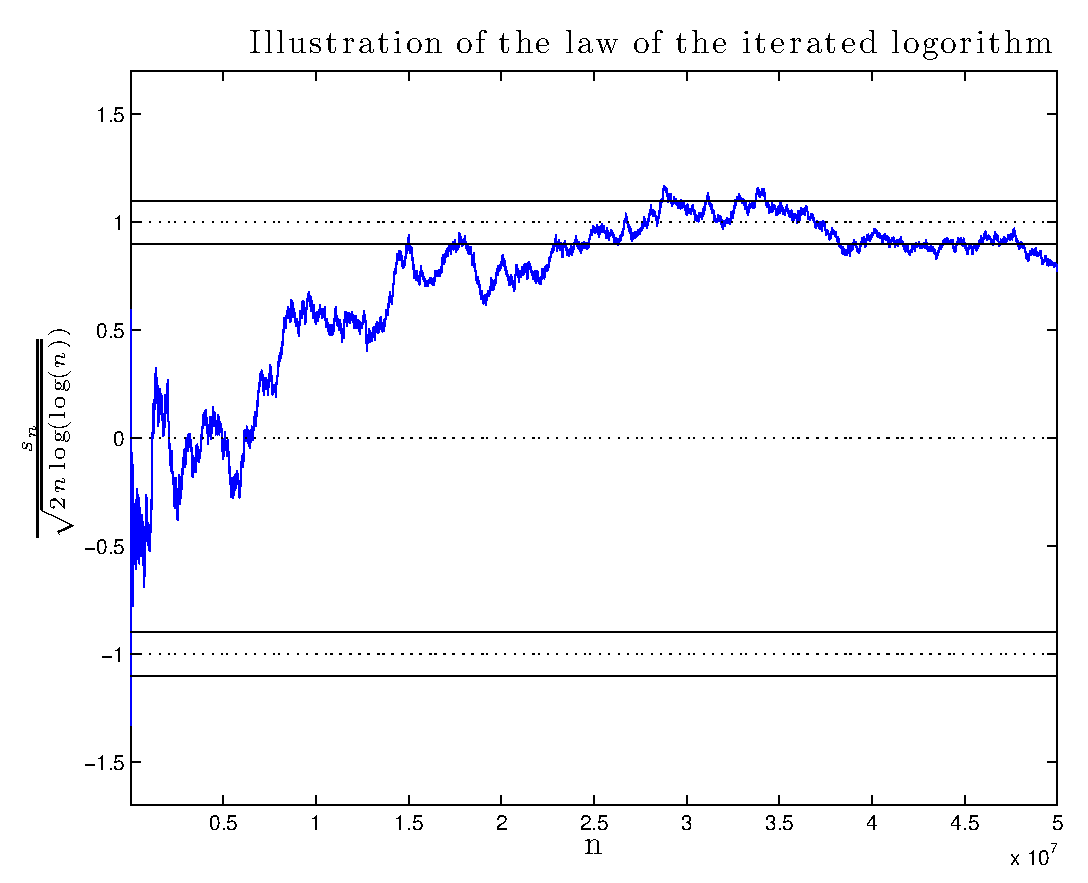
\includegraphics[height = 2.7in]{Measure/LIL.eps}
\end{figure}


\begin{lemma}
\label{LIIL: io lemma 1}
For all $\epsilon > 0 $
\begin{align*}
P[ s_n/\ell_n \geq  (1+\epsilon) \io_n ] = 0
\end{align*}
\end{lemma}
\begin{proof}
The obvious strategy is to use the first Borel-Cantelli lemma. In particular, it would be nice if we could show
\[
\sum_{n=1}^\infty P [ s_n/\ell_n \geq  (1+\epsilon)]<\infty
\]
which would give us the lemma. By the first half of the large deviation result we know $P [ s_n/\ell_n \geq  (1+\epsilon)]$ converge to zero as $n\rightarrow \infty$. Unfortunately, they do not converge fast enough for the first Borel-Cantelli. Taking a sub-sequence will get something summable but we would need to show that the events are well behaved between the sub-sequence. Fortunatly we can do this since the sets $\{s_n/\ell_n \geq  (1+\epsilon)\}$ overlap a lot. The strategy is to group the events $\{s_n/\ell_n \geq  (1+\epsilon)\}$ by unioning them into blocks, then apply Borel-Cantelli on the blocks. This will be sufficient since  the blocks occur infinity often if and only if the events $s_n/\ell_n \geq  (1+\epsilon)$ occur infinity often.  Controlling the probability of the blocks is done with the maximal inequality.

Let the $k^\text{th}$ block be defined
\[
B_k:= \bigcup_{j=n_{k-1}}^{n_k} \{ s_{j}/\ell_{j} \geq  (1+\epsilon) \}
\]
  where $n_k$ is  a (yet to be determined) subsequence. We  use maximal inequality  to bound $P[B_k]$ as follows
\begin{align*}
P[B_k]  &\leq P[\max_{n_{k-1}\leq j\leq n_k} s_j \geq (1+\epsilon)\min_{n_{k-1}\leq j\leq n_k} \ell_{j}] \\
 &\leq P[\max_{n_{k-1}\leq j\leq n_k} s_j \geq (1+\epsilon) \ell_{n_{k-1}}] \\
 &\leq P[\max_{j\leq n_k} s_j \geq (1+\epsilon) \ell_{n_{k-1}}] \\
 &\leq P[\max_{j\leq n_k} s_j \geq \lceil(1+\epsilon) \ell_{n_{k-1}}\rceil],\quad\text{since $s_j\in\Bbb Z$} \\
 &\leq 2P[ s_{n_k} \geq \lceil(1+\epsilon) \ell_{n_{k-1}}\rceil],\quad\text{maximal ineq} \\
 &\leq 2P[ s_{n_k} \geq (1+\epsilon) \ell_{n_{k-1}}] \\
 &\leq \exp\bigl( - \textstyle\frac{1}{2}(1+\epsilon)^2 \ell^2_{n_{k-1}}/n_{k} \bigr),\quad\text{half of large deviation}\\
 &\leq \exp\bigl( - (1+\epsilon)^2 n_{k-1}\log\log n_{k-1}/n_{k} \bigr)\\
 & = \left(\frac{1}{\log n_{k-1}} \right)^{ (1+\epsilon)^2\frac{n_{k-1}}{n_{k}} }.
\end{align*}
Now we just find $n_k$ which makes the last term summable over $k$. If $n_k\approx \theta^k$ one gets
\begin{align*}
\left(\frac{1}{\log n_{k-1}} \right)^{ (1+\epsilon)^2\frac{n_{k-1}}{n_{k}} }
& \approx  \left(\frac{1}{(k-1)\log\theta} \right)^{ (1+\epsilon)^2\frac{1}{\theta} }
\end{align*}
which is summable if $(1+\epsilon)^2\frac{1}{\theta} >1$. We also need that   $\theta > 1$  since we need $n_k\rightarrow \infty$ as $k\rightarrow \infty$. Luckily there does exist such a $\theta$ for which $(1+\epsilon)^2> \theta > 1$.
\end{proof}

\begin{lemma}
\label{LIIL: io lemma 2}
For all $\epsilon >0 $
\begin{align*}
P[ s_n/\ell_n > (1-\epsilon) \io_n ] = 1
\end{align*}
\end{lemma}
\begin{proof}
In the previous lemma we presented a technique to adjust the first Borel-Cantelli lemma in the case the summability condition doesn't hold. For this  lemma we want to use the second Borel-Cantelli lemma but, again, it doesn't directly apply since the condition that the events $s_n/\ell_n > (1-\epsilon)$ are independent does not hold. Here is a generic technique to get around this obstacle. Find subsequence $n_k$ and subsets
\[
I_k \subset   \{s_{n_k}/\ell_{n_k} > (1-\epsilon)\}
\]
such that $I_k$'s  are independent and $\sum_k P[I_k]=\infty$ so that $P[I_k \io_k]=1$ (which would then give the lemma). Unfortunately, even this doesn't work. What ends up working is to find two sets $A_k$ $I_k$ such that
\begin{align}
&A_k\cap I_k \subset \{s_{n_k}/\ell_{n_k} > (1-\epsilon)\}  \label{ABns in wwt}\\
&\text{$I_k$ are independent and $\textstyle\sum_k P[I_k]=\infty$} \label{Bns ind}\\
&\text{$A_k$ are not independent but $P[A_k \aall_k] = 1$.}\label{Ans Borel}
\end{align}
To see why this is sufficient notice that (\ref{Bns ind}) implies $P[I_k \io_k] = 1$ by the second Borel-Cantelli lemma. Then
\begin{align*}
&\text{ $P[A_k \aall_k] = 1$ and $P[I_k \io_k]=1$ } \\
&\qquad\Longrightarrow P[A_k \cap I_k \io_k] = 1 \\
&\qquad\overset{(\ref{ABns in wwt})}\Longrightarrow  P[s_{n_k}/\ell_{n_k} > (1-\epsilon) \io_k] = 1
\end{align*}
Therefore (\ref{ABns in wwt}), (\ref{Bns ind}) and (\ref{Ans Borel}) are sufficient to establish the lemma.

Figuring out how to define $I_k$ and $A_k$ are the tricky parts. The intuition is that if your going to get independent events you need to look at increments of $s_{n}$. Define
\begin{align*}
I_k &:= \{s_{n_k}-s_{n_{k-1}} \geq (1-\epsilon/2)\ell_{n_k}  \} \\
A_k &:= \{ s_{n_{k-1}} > -(\epsilon/2)\ell_{n_k}  \}.
\end{align*}
Clearly  $I_k \cap A_k \subset \{s_{n_k}/\ell_{n_k} > (1-\epsilon)\}$ so that (\ref{ABns in wwt}) holds. Moreover, the $I_k$'s  are independent.
To show (\ref{Ans Borel})
\begin{align*}
P[A_k \aall_k] &= P\Bigl[s_{n_{k-1}} > -(\epsilon/2)\ell_{n_k} \aall_k\Bigr] \\
 &= P\Bigl[s_{n_{k-1}} < (\epsilon/2)\ell_{n_k} \aall_k\Bigr],\quad\text{by symmetry} \\
&= P\Bigl[\frac{s_{n_{k-1}}}{\ell_{n_{k-1}}} < (\epsilon/2)\frac{ \ell_{n_k} }{ \ell_{n_{k-1}} } \aall_k\Bigr] \\
&= 1- P\Bigl[\frac{s_{n_{k-1}}}{\ell_{n_{k-1}}} \geq (\epsilon/2)\frac{ \ell_{n_k} }{ \ell_{n_{k-1}} } \io_k\Bigr] \\
&= 1,\,\text{by Lemma \ref{LIIL: io lemma 1} if \textcolor{blue}{$\frac{\ell_{n_k}}{\ell_{n_{k-1}}}\rightarrow \infty$.}}
\end{align*}
To show (\ref{Bns ind}) notice
\begin{align}
P[I_k] &= P\Bigl[ s_{n_k}-s_{n_{k-1}}\geq(1-\epsilon/2)\ell_{n_k}\Bigr] \nonumber\\
&= P\Bigl[s_{n_k-n_{k-1}}\geq(1-\epsilon/2)\ell_{n_k}\Bigr] \nonumber\\
&\geq P\Bigl[\frac{s_{n_k-n_{k-1}}}{\sqrt{n_k - n_{k-1}}}  \geq \frac{(1-\epsilon/2)\ell_{n_k}}{\sqrt{n_k - n_{k-1}}} \Bigr] \nonumber\\
&\geq \exp\Bigl(-\frac{1}{2}\Bigl[\frac{(1-\epsilon/2)\ell_{n_k}}{\sqrt{n_k - n_{k-1}}}\Bigr]^2(1+o(1))  \Bigr),\label{make this diverge}\\
&\qquad\qquad\text{\textcolor{blue}{by Lemma \ref{LIL: usefull lemma 2} if:}}\nonumber\\
&\qquad\qquad\quad\text{ \textcolor{blue}{$\textstyle\frac{\ell_{n_k}}{\sqrt{n_k - n_{k-1}}}\rightarrow \infty$ and  }}\nonumber\\
&\qquad\qquad\quad\text{ \textcolor{blue}{$\textstyle\frac{1}{\sqrt{n_k - n_{k-1}}}\frac{\ell_{n_k}}{\sqrt{n_k - n_{k-1}}}\rightarrow 0$ and }}\nonumber\\
&\qquad\qquad\quad\text{ \textcolor{blue}{$n_k - n_{k-1}\rightarrow \infty$. }}\nonumber
\end{align}
To finish the proof of (\ref{Ans Borel}) and (\ref{Bns ind}) we need to find $n_k\rightarrow \infty$ such that $\ell_{n_k}$ satisfies the above conditions and the \textcolor{blue}{sum of (\ref{make this diverge}) diverges}.

A subsequence of the form $n_k := \lfloor\exp(k^\theta)\rfloor$ will work. To check the conditions notice

\begin{align*}
\frac{\ell_{n_k}}{\ell_{n_{k-1}}}
& \sim \frac{ \sqrt{2 \exp(k^\theta) \log k^\theta} }{\sqrt{2 \exp((k-1)^\theta) \log (k-1)^\theta}} \\
& =  \exp\Bigl(\frac{k^\theta - (k-1)^\theta}{2}\Bigr) \frac{\log k}{\log (k-1)}  \\
& =  \exp\Bigl(\frac{\theta(k^*)^{\theta-1}}{2}\Bigr) (1 + o(1)),\quad\text{where $k-1\leq k^*\leq k$} \\
& \longrightarrow  \infty, \quad\text{\textcolor{red}{if  $\theta > 1$}.}
\end{align*}
Also
\begin{align*}
n_k - n_{k-1} & \sim  \exp(k^\theta) - \exp((k-1)^\theta) \\
&= \theta (k^*)^{(\theta-1)} \exp((k^*)^\theta) ,\quad\text{where $k-1\leq k^*\leq k$} \\
&\longrightarrow \infty,\quad\text{\textcolor{red}{if $\theta > 0 $.}}
\end{align*}
And therefore
\begin{align*}
\frac{\ell_{n_k}}{\sqrt{n_k - n_{k-1}}}
& \sim \frac{\sqrt{2 \exp(k^\theta) \log k^\theta}}{\sqrt{ \exp(k^\theta) - \exp((k-1)^\theta) }}   \\
&  = \frac{\sqrt{2\theta\log k}}{\sqrt{ 1 - \exp((k-1)^\theta-k^\theta)  }}  \\
& = \frac{\sqrt{2\theta\log k}}{\sqrt{ 1 - o(1)  }}\\
& \longrightarrow \infty.
\end{align*}
Clearly we now have that  $\frac{\ell_{n_k}}{{n_k - n_{k-1}}}  \longrightarrow 0.$
Finally we need to show that the sum of (\ref{make this diverge}) over $k$ diverges.  The individual terms are
\begin{align*}
\exp\Bigl(-\frac{1}{2}\Bigl[&\frac{(1-\epsilon/2)\ell_{n_k}}{\sqrt{n_k - n_{k-1}}}\Bigr]^2(1+o(1))  \Bigr) \\
& \sim \exp\Bigl(-\frac{(1-\epsilon/2)^2}{2}2\theta \log k   \Bigr) \\
& = \exp\Bigl(-{(1-\epsilon/2)^2}\theta \log k   \Bigr) \\
& = k ^ {-{(1-\epsilon/2)^2}\theta}
\end{align*}
the sum of the above terms over $k$ diverges if $(1-\epsilon/2)^\theta  < 1$, i.e. \textcolor{red}{ if $\theta < \frac{1}{(1-\epsilon)^2}$}. Now putting all the  conditions on $\theta$ together says that we simply need to choose $\theta$ such that
\[ 1<\theta <\frac{1}{(1-\epsilon/2)^2} .\]
\end{proof}


%%%%%%%%%%%%%%%%%%%%%%%%%%%%%%%%%%%%%%%%%%%%%%
\clearpage
\part{Integration}

%-------------------------------'
%---------section  ---------------'
%-------------------------------'
\section{Measurable functions}
%-------------------------------'
%---------section  ---------------'
%-------------------------------'

%\subsection{Basic theory}

\begin{definition}[{\bf Measurable functions}]
If $(\Omega_1, \mathcal F_1)$ and $(\Omega_2,\mathcal F_2)$ are measurable spaces then $f\colon \Omega_1 \rightarrow \Omega_2$ is said to be {measurable between $\mathcal F_1$ and $\mathcal F_2$} (written $f\mcirc \mathcal F_1/\mathcal F_2$) if and only if
\[ f^{-1}(A)\in \mathcal F_1,\quad\forall A\in\mathcal F_2\]
where $ f^{-1}(A):=\{w\in\Omega_1: f(w)\in A \}$.
\end{definition}


\begin{theorem}[{\bf Basic facts about pull backs}]
\label{thm pull back basic facts}
Let $f\colon \Omega_1 \rightarrow \Omega_2$. Let $A, A_1, A_2, \ldots \subset \Omega_2$. Then
\begin{itemize}
\item $f^{-1}(\Omega_2) = \Omega_1$
\item $f^{-1}(\varnothing) = \varnothing$
\item $f^{-1}(\Omega_2 - A) = \Omega_1 - f^{-1}(A)$
\item $f^{-1}(\cup_i A_i) =  \cup_i  f^{-1}(A_i)$
\item $f^{-1}(\cap_i A_i) = \cap_i  f^{-1}(A_i)$.
\end{itemize}
\end{theorem}
\begin{proof} These are very easy to check. For example  to see why $f^{-1}(\cup_i A_i) \subset  \cup_i  f^{-1}(A_i)$ notice that
\begin{align*}
\omega \in f^{-1}(\cup_i A_i)
&\Longrightarrow f(\omega) \in \cup_i A_i \\
&\Longrightarrow \text{$f(\omega) \in A_i$ for some $i$ }\\
&\Longrightarrow \text{$\omega \in f^{-1}(A_i)$ for some $i$ }\\
&\Longrightarrow \omega \in \cup_i f^{-1}(A_i).
\end{align*}
The other arguments are exactly similar.
\end{proof}


\begin{theorem}[{\bf Generators are enough}]
\label{thm: GaE}
Let $(\Omega_1, \mathcal F_1)$ and $(\Omega_2,\mathcal F_2)$ be  measurable spaces where $\mathcal F_2$ is generated by some class $\mathcal A\subset 2^{\Omega_2}$ (i.e. $\mathcal F_2=\sigma\langle \mathcal A\rangle$). If $f:\Omega_1\rightarrow \Omega_2$ then
\[ f \mcirc \mathcal F_1/\mathcal F_2 \Longleftrightarrow f^{-1}(A)\in\mathcal F_1,\,\, \forall A\in\mathcal A.\]
\end{theorem}



\begin{corollary}[{\bf Monotone real maps are measurable}]
Any monotone map $f\colon \Bbb R\rightarrow \Bbb R$ is measurable $\mathcal B^{\Bbb R}/\mathcal B^{\Bbb R}$.
\end{corollary}

\begin{corollary}[{\bf Continuous real maps are measurable}]
Any continuous map $f\colon \Bbb R^d\rightarrow \Bbb R^k$ is measurable $\mathcal B^{\Bbb R^d}/\mathcal B^{\Bbb R^k}$.
\end{corollary}




\begin{theorem}[{\bf Composition of $\mcirc$ functions is $\mcirc$}]
\label{thm: composition of measurable}
Let $(\Omega_1,\mathcal F_1)$, $(\Omega_2,\mathcal F_2)$ and $(\Omega_3,\mathcal F_3)$ be measurable spaces. Suppose $f$ and $g$ are functions sending $\Omega_1\overset{f} \longmapsto \Omega_2 \overset{g}\longmapsto \Omega_3$. If $f\mcirc \mathcal F_1/\mathcal F_2$ and $g\mcirc  \mathcal F_2/\mathcal F_3$ then $g\circ f \mcirc\mathcal F_1/\mathcal F_3$.
\end{theorem}


\begin{corollary}[{\bf Just check that each coordinate is $\mcirc$}]
\label{coordM}
Let $(\Omega,\mathcal F)$ be a measurable space and $f:\Omega\rightarrow \Bbb R^d$. Let $f=(f_1,\ldots, f_d)$ decompose $f$ into the coordinate functions (so that $f_k:\Omega\rightarrow \Bbb R$). Then
\[ f\mcirc \mathcal F/\mathcal B^{\Bbb R^d}\Longleftrightarrow  f_k\mcirc \mathcal F/\mathcal B^{\Bbb R}, \text{ for each $k$.} \]
\end{corollary}



\begin{theorem}[{\bf Scissors and paste}]
Let $(\Omega_1, \mathcal F_1)$ and $(\Omega_2,\mathcal F_2)$ be measurable spaces and $f\colon \Omega_1 \rightarrow \Omega_2$.  In addition, suppose there exists $\mathcal F_1$-sets $A_1,A_2,\ldots$ such that $\Omega_1 = \cup_{k=1}^\infty A_k$. Then
\[ f\mcirc \mathcal F_1/\mathcal F_2 \Longleftrightarrow  f\bigr|_{A_k} \mcirc (\mathcal F_1\!\cap\! A_k)/\mathcal F_2, \text{ for each $k$.} \]
\end{theorem}

\begin{corollary}[{\bf Piecewise-continuous real maps are measurable}]
Any map $f\colon \Bbb R^d\rightarrow \Bbb R^k$ which is piecewise continuous on each piece of a  countable-measurable-partition of $\Bbb R^d$  is measurable $\mathcal B^{\Bbb R^d}/\mathcal B^{\Bbb R^k}$.
\end{corollary}


\begin{theorem}[{\bf Metric-continuous functions  are measurable}]
Suppose $\Omega_1$ and $\Omega_2$ are metric spaces and $f$ is a function mapping $\Omega_1$ into $\Omega_2$.
If there exists $\mathcal B^{\Omega_1}$ sets $A_1,A_2,\ldots$ such that $\Omega_1=\cup_{k=1}^\infty A_k$ and $f\bigr|_{A_k}$ is continuous (with respect to the induced metrics) on each $A_k$ then $f$ is measurable $\mathcal B^{\Omega_1}/\mathcal B^{\Omega_2}$.
\end{theorem}


\begin{theorem}[{\bf Just check Borel $\mcirc$ on the range}]
Let $(\Omega_1, \mathcal F_1)$ be a measurable space and $\Omega_2$ be a metric space.
Suppose $f$ is a function which maps $\Omega_1$ into $\Omega_{2}^o\subset \Omega_2$. Then
\[ f\mcirc \mathcal F_1/\mathcal B^{\Omega_2^o} \Longleftrightarrow f\mcirc \mathcal F_1/\mathcal B^{\Omega_2}  \]
where the metric used to define $\mathcal B^{\Omega_2^o}$ is the one induced by the metric on $\Omega_2$.
\end{theorem}

\begin{definition}[{\bf Nomenclature for the extended reals}]\label{nonmen}
$\vphantom{asdf}$
\begin{itemize}
\item $\mathcal B$ is shorthand notation for $\mathcal B^{\bar{\Bbb R}}$.
\item If $(\Omega, \mathcal F)$  is a measurable space and $f:\Omega \rightarrow \bar{\Bbb R}$ we use the nomenclature  `$\mcirc \mathcal F$' or just `measurable $\mathcal F$' as short hand for $\mcirc \mathcal F/\mathcal B$.
\item We say that a function $f$ is `Borel measurable' or just `measurable' if $f:\Bbb R^d \rightarrow \bar{\Bbb R}$ and $f$ is $\mcirc {\mathcal B^{\Bbb R^d}}/\mathcal B$.
\item We say that a function $f$ is `Lebesque measurable'  if $f:\Bbb R^d \rightarrow \bar{\Bbb R}$ and $f$ is $\mcirc \overline{\mathcal B^{\Bbb R^d}}/\mathcal B$.
\end{itemize}
\end{definition}

\begin{definition}[{\bf Defining algebraic operations with $\infty$}]
$\vphantom{asdf}$
\begin{itemize}
\item $\infty + c := \infty$  for any $-\infty< c\leq \infty$.
\item $\infty\cdot 0 =0\cdot\infty:=0$.
\item $\infty\cdot \infty := \infty$.
\item $\frac{c}{\infty}:=0$ when $c\in \Bbb R$.
\item $\frac{c}{0}$, $\frac{\pm\infty}{\pm\infty}$,  $\infty - \infty$ and $-\infty + \infty$ are not defined.
\end{itemize}
\end{definition}

\begin{theorem}[{\bf Closure theorem for $\mcirc$ functions}]
If $(\Omega, \mathcal F)$ is a measurable space then
\begin{enumerate}
\item If $f$ and $g$ are  $\mcirc \mathcal F$ functions then $cf$ (c is a constant), $f+g$, $fg$, $f/g$, $f\vee g$, $f\wedge g$, $f^+$, $f^-$ are each $\mcirc \mathcal F$, provided the composite function are defined at every $w\in\Omega$.
\item If $f_1, f_2,\ldots $  $\mcirc \mathcal F$ functions then $\sup_n f_n$, $\inf_n f_n$, $\limsup_n f_n$, $\liminf_n f_n$ are each $\mcirc \mathcal F$.
\end{enumerate}
\end{theorem}



\begin{definition}[{\bf Simple functions}]
Let $(\Omega, \mathcal F)$ denote a measurable space. Then
any function $f\colon \Omega \rightarrow \bar{\Bbb R}$ which is $\mcirc \mathcal F$ and has a finite range is called a {simple function}.
\end{definition}


\begin{definition}[{\bf Characterization of simple functions}]
Let $(\Omega, \mathcal F)$ denote a measurable space and suppose  $f\colon \Omega \rightarrow \bar{\Bbb R}$. Then $f$ is a simple function if and only if there exists a finite partition of $\Omega$ into disjoint $\mathcal F$-sets $A_1,\ldots, A_n$
and a finite list of extended real numbers $c_1,\ldots, c_n$
 such that $f=\sum_{k=1}^n c_k I_{A_k}$.
\end{definition}





\begin{definition}[{\bf $\mathscr N_s$ and $\mathscr N$}]
Let $(\Omega, \mathcal F)$ denote a measurable space. Then
\begin{itemize}
\item $\mathscr N_s$ denotes the set of non-negative simple functions \mbox{$f:\Omega\rightarrow \bR$}.
\item $\mathscr N$ denotes the set of non-negative functions $f:\Omega\rightarrow \bR$ which are  $\mcirc \mathcal F$.
\end{itemize}
\end{definition}



\begin{theorem}[{\bf The structure theorem}]
\label{thm: structure thm}
Let $(\Omega, \mathcal F)$ be a measurable space and suppose $f\colon \Omega\rightarrow \bar{\Bbb R}$ is $\mcirc \mathcal F$. Then
\begin{enumerate}
\item There exists bounded simple functions $f_1, f_2,\ldots $ such that $\lim_n f_n(w)= f(w)$ for each $w\in \Omega$.
\item If, in addition,  $f\in\mathscr N$  then there exists bounded $f_1, f_2, \ldots \in\mathscr N_s$ such that $ f_n(w)\uparrow f(w)$ for each $w\in \Omega$.
\end{enumerate}
\end{theorem}


\begin{exercise} Show that Corollary \ref{coordM} holds for functions mapping into $\bar{\Bbb R}^d$.
\end{exercise}


\begin{exercise}
Let $(\Omega, \mathcal F)$ be a measure space and let $f_0, f_1,\ldots$ be an infinite sequence of $\mathcal F$-measurable functions of $\Omega$. Show that the radius $R$ of convergence of the random power series $\sum_{k=0}^\infty f_k x^k$ is an $\mathcal F$-measurable function of $\Omega$.
\end{exercise}


\begin{exercise}
Give an example of two measurable spaces $(\Omega_1, \mathcal F_1)$,  $(\Omega_2,\mathcal F_2)$, a $\mcirc \mathcal F_1/\mathcal F_2$ mapping $f:\Omega_1\rightarrow \Omega_2$,  and an event $B\in\mathcal F_1$ such that $f(B)\notin \mathcal F_2$.
\end{exercise}



%%%%%%%%%%%%%%%%%
%
%  random variable subsection
%
%%%%%%%%%%%%%%%%%%%%%
\subsection{Application: Random variables and distribution functions }



\begin{theorem}[{\bf Induced measures}]
Let $(\Omega_1, \mathcal F_1)$ and $(\Omega_2,\mathcal F_2)$ be two measurable spaces. Suppose $f:\Omega_1\rightarrow \Omega_2$ is $\mcirc \mathcal F_1/\mathcal F_2$ and $\mu$ is a measure on $\Omega_1$. Then the set function defined by
\[ \mu f^{-1}(B):=\mu(f^{-1}(B)),\quad\text{for all $B\in\mathcal F_2$}\]
 is a measure on $(\Omega_2,\mathcal F_2)$ and is called the {\bf induced measure} on $(\Omega_2,\mathcal F_2)$. Moreover,
 \begin{align*}
 &\bullet\text{$\mu$ is a probability measure} \Longrightarrow  \text{$\mu f^{-1}$ is a probability measure;}\\
 &\bullet\text{$\mu$ is a finite measure} \Longrightarrow  \text{$\mu f^{-1}$ is a finite measure;} \\
 &\bullet\text{$\mu$ is a $\sigma$-finite measure} \not\Longrightarrow  \text{$\mu f^{-1}$ is a $\sigma$-finite measure.}
 \end{align*}
\end{theorem}


Give example of where the induced measure is not $\sigma$-finite but the base measure is.



\begin{definition}[{\bf Random variable}]
Any function $X\colon \Omega \rightarrow \Bbb R$ which is measurable $\mathcal F/\mathcal B^{\Bbb R}$  is said to be a {\bf random variable}.
\end{definition}

Distribution function are useful for making random variables with the specified induced distribution.

\begin{definition}[{\bf Distribution function on $\Bbb R$}]
A function $F\colon\Bbb R\rightarrow\Bbb R$ if called a {\bf distribution function} if $F$ satisfies the following three requirements:
\begin{itemize}
\item $F$ is non-decreasing;
\item $F$ is right continuous;
\item $\lim_{x\rightarrow \infty} F(x)=1$ and $\lim_{x\rightarrow -\infty} F(x)=0$.
\end{itemize}
\end{definition}


\begin{theorem}[{\bf Df's determine $PX^{-1}$}]
If $F$ is a distribution function then there exists a random variable $X$ defined on some probability space $(\Omega, \mathcal F, P)$ such that
\[ P(X\leq x) = F(x)\text{ for all $x\in\Bbb R$}. \]
Moreover, the distribution of $X$ is uniquely determined by $F$.
\end{theorem}


\begin{theorem}[{\bf $F^{-1}(U)\sim X$}]
Let $X$ be a random variable and define $F(x):=P(X\leq x)$. Let $U$ be a random variable uniformly distributed over $(0,1)$.  Then $F$ is a distribution function and $F^{-1}(U)\sim X$ (i.e. $F^{-1}(U)$ and $X$ have the same induced distribution on $\Bbb R$) where
\begin{equation}
\label{inverse CDF definition}
F^{-1}(u):=\inf\{x\in\Bbb R\colon u\leq F(x)  \}.
\end{equation}
\end{theorem}


\begin{theorem}[{\bf  $F(X)\sim U$}]
Let $X$ be a random variable with distribution function $F(x)=P(X\leq x)$. Then
\[ P(F(X)\leq u)\leq u\text{ for all $0<u<1$.} \]
Moreover, $F$ is continuous if and only if $P(F(X)\leq u)= u$ for all $0<u<1$.
\end{theorem}




\clearpage
%%%%%%%%%%%%%%%%%%%%%%%%%%%%%%
%
%  section
%
%%%%%%%%%%%%%%%%%%%%%%%%%%%%%%%%%%%%%%
\section{$\sigma$-fields generated by functions}



The results here will be used often in the later text. We will use them for generating a product measure, for Fubini's theorem and for conditional expected value.





\begin{definition}[{\bf The $\sigma$-field generated by functions}]
\label{def: sig generated by funs}
Let $\mathcal I$ be an arbitrary index set.
Let $(\Omega_i, \mathcal F_i)$ be a collection of measurable spaces indexed by $i\in \mathcal I$.
Let $f_i:\Omega \rightarrow \Omega_i$ be a  collection of functions indexed by $i\in \mathcal I$. Then the {\bf $\sigma$-field generated by $\{f_i: i\in\mathcal I\}$} is defined as
\[ \sigma\langle  f_i, \mathcal F_i:i\in \mathcal I \rangle :=  \bigcap_{\shortstack{\text{\small $\mathcal F$ is a $\sigma$-field on $\Omega$}  \\
 \text{\small each $X_i$ is $\mcirc \mathcal F/\mathcal F_i$ }}}\mathcal F\]
 and corresponds to the smallest $\sigma$-field  on $\Omega$ which makes all the random variables $f_i$ measurable.
 \end{definition}


When $\mathcal F_i$ are clear from context we may, and do, write
\[
\text{
$\sigma\langle f_i\colon i\in\mathcal I \rangle$ as shorthand for $\sigma\langle f_i, \mathcal F_i\colon i\in\mathcal I \rangle$.
}
\]


\begin{theorem}[{\bf Pull back for one map}]
For a single function $f_1:\Omega \rightarrow \Omega_1$ where $(\Omega_1, \mathcal F_1)$ is a measurable space one has that $\sigma \langle f_1,\mathcal F_1\rangle = f^{-1}(\mathcal F_1):= \{f^{-1}(F)\colon F\in \mathcal F_1 \}$.
\end{theorem}
\begin{proof}
We immediately have that $f^{-1}(\mathcal F_1)\subset \sigma \langle f_1,\mathcal F_1\rangle$ since by definition $f$ is  $\mcirc \sigma \langle f_1,\mathcal F_1\rangle/\mathcal F_1$.
To show $\sigma \langle f_1,\mathcal F_1\rangle\subset f^{-1}(\mathcal F_1)$, all we need is to establish that $f^{-1}(\mathcal F_1)$ is a $\sigma$-field (since trivially $f$ is  $\mcirc f^{-1}(\mathcal F_1)/\mathcal F_1$). This is easily checked by the properties of pull-back sets given in Theorem \ref{thm pull back basic facts}.
\end{proof}


\begin{theorem}[{\bf Generators are enough}]
If, in addition to the assumptions presented in Definition \ref{def: sig generated by funs}, one has that each $\mathcal F_i = \sigma\langle \mathcal A_i \rangle$, then
\[\sigma\langle f_i, \mathcal F_i\colon i\in \mathcal I\rangle = \sigma \bigl\langle f_i^{-1}(A_i)\colon A_i\in \mathcal A_i, i\in \mathcal I \bigr\rangle. \]
\end{theorem}
\begin{proof}
The only interesting direction is to show $\sigma\langle f_i, \mathcal F_i\colon i\in \mathcal I\rangle \subset \sigma \bigl\langle f_i^{-1}(A_i)\colon A_i\in \mathcal A_i, i\in \mathcal I \bigr\rangle$. By ``good sets'' we just need to show that each $f_i$ is $\mcirc \sigma \bigl\langle f_i^{-1}(A_i)\colon A_i\in \mathcal A_i, i\in \mathcal I \bigr\rangle / \sigma\langle\mathcal A_i\rangle$. This follows immediately from Theorem \ref{thm: GaE} (generators are enough).
\end{proof}




\begin{definition}[{\bf The product $\sigma$-field}]
Let $\mathcal I$ be an arbitrary index set. Let $(\Omega_i, \mathcal F_i)$ be a collection of measurable spaces indexed by $i\in \mathcal I$. Define the product $\sigma$-field on $\prod_{i\in \mathcal I}\Omega_i$  to be
\[
\textstyle\bigotimes_{i\in\mathcal I} \mathcal F_i := \sigma\langle \pi_i,\mathcal F_i\colon i\in \mathcal I \rangle
\]
where $\pi_i\colon \Omega \rightarrow \Omega_i$ is defined as the $i^\text{th}$ coordinate mapping (e.g. $\pi_i(\omega_1, \omega_2,\ldots) = \omega_i$).
 \end{definition}


\begin{theorem}[{\bf Clump $f_i$ into a vector map}]
\label{thm: clump}
Let $(\Omega, \mathcal F)$ be a measurable space.
Let $(\Omega_i, \mathcal F_i)$ be a collection of measurable spaces indexed by an arbitrary index set $\mathcal I$ and let $f_i:\Omega\rightarrow \Omega_i$. Define $\vec f\colon \Omega \rightarrow \prod_{i\in \mathcal I} \Omega_i$ to be the map which sends $\omega \overset{\vec f}\mapsto (f_i(\omega))_{i\in\mathcal I}$. Then
\[
\text{$\vec f$ is $\mcirc \mathcal F / \textstyle\bigotimes_{i\in\mathcal I} \mathcal F_i$}
\Longleftrightarrow
\text{each $f_i \mcirc \mathcal F/\mathcal F_i$}.
\] Moreover, $\sigma\langle f_i,\mathcal F_i\colon i\in\mathcal I \rangle = \vec f^{-1}\bigl(\bigotimes_{i\in\mathcal I} \mathcal F_i\bigr)$.
\end{theorem}


\begin{theorem}[{\bf Measurable with respect to $\sigma\langle f_i \rangle$}]
\label{thm: f = g(vec f)}
Using the same assumptions and notation as in Definition \ref{def: sig generated by funs},
a function $f\colon\Omega\rightarrow \bar{\Bbb R}$ is measurable $\sigma\langle  f_i, \mathcal F_i:i\in \mathcal I \rangle$ if and only if there exists a function $g\colon \prod_{i\in \mathcal I} \Omega_i\rightarrow \bar{\Bbb R}$ which is measurable $\bigotimes_{i\in\mathcal I}\mathcal F_i$ and  $f= g((f_{i})_{i\in\mathcal I})$.
\end{theorem}
\begin{proof}
($\Longleftarrow$) This follows directly from Theorem \ref{thm: clump} (clump theorem) and Theorem \ref{thm: composition of measurable} (composition of measurable is measurable).

($\Longrightarrow$) This follow by an application of the $1-2-3$ argument. In particular, we show the result for simple function, then extend by taking point-wise limits. To start let $\vec f := (f_i)_{i\in \mathcal I}$ denote the clumped vector map. To summarize what is know from the assumptions and  \ref{thm: clump}
\begin{itemize}
\item $f\colon \Omega \rightarrow \bar{\Bbb R}$ is $\mcirc \sigma\langle f_i, \mathcal F_i\colon i\in\mathcal I \rangle/\mathcal B$;
\item $\vec f\colon \Omega \rightarrow \prod_{i\in\mathcal I}\Omega_i$ is $\mcirc \sigma\langle f_i, \mathcal F_i\colon i\in\mathcal I \rangle/\bigotimes_{i\in \mathcal I} \mathcal F_i$.
\item $\sigma\langle f_i, \mathcal F_i\colon i\in\mathcal I \rangle = \vec f^{-1}\bigl(\bigotimes_{i\in \mathcal I} \mathcal F_i\bigr)$
\end{itemize}


Suppose that $f=\sum_{k=1}^n c_k I_{A_k}$ for $A_k\in \sigma\langle f_i, \mathcal F_i\colon i\in\mathcal I \rangle = \vec f^{-1}\bigl(\bigotimes_{i\in \mathcal I} \mathcal F_i\bigr)$. Since $\sigma\langle f_i, \mathcal F_i\colon i\in\mathcal I \rangle = \vec f^{-1}\bigl(\bigotimes_{i\in \mathcal I} \mathcal F_i\bigr)$ we can write $A_k= \vec f^{-1} (F_k)$ where $F_k\in \bigotimes_{i\in \mathcal I} \mathcal F_i$. Now
\begin{align*}
f=\sum_{k=1}^n c_k I_{A_k} =\sum_{k=1}^n c_k I_{\vec f^{-1} (F_k)} =\sum_{k=1}^n c_k I_{F_k} \circ \vec f= g \circ \vec f
\end{align*}
where $g:=\sum_{k=1}^n c_k I_{F_k}$.
Certainly $g$ is $\mcirc \bigotimes_{i\in \mathcal I} \mathcal F_i / \mathcal B$ as was to be shown.

To finish let $f$ be a arbitrary $\mcirc \sigma\langle f_i, \mathcal F_i\colon i\in\mathcal I \rangle/\mathcal B$ function. By Theorem \ref{thm: structure thm} (the structure theorem) we can write $f(\omega) = \lim f_n(\omega)$ where $f_n$ are bounded simple functions. Therefore, from the preivous case, there exists $g_n$ which are $\mcirc \bigotimes_{i\in \mathcal I} \mathcal F_i / \mathcal B$ and $f_n(\omega) = g_n(\vec f(\omega))$. We definitely have that $f(\omega) = \lim f_n(\omega) = \lim g_n(\vec f(\omega))$ at each $\omega$. However we are not exactly done since there is no reason that $\lim_n g_n(v)$ exists for $v$'s which are not of the form $v=\vec f(\omega)$ (and therefore setting $g(v):=\lim g_n(v)$ only defines $g$ on the range of $\vec f$ ). To get around this set
\[
g(v):=\begin{cases}
\limsup_ng_n(v), &\text{when $\limsup_ng_n(v) =  \liminf_ng_n(v)$}\\
0, &\text{otherwise}.
\end{cases}
\]
This $g$ definitely satisfies $f = g \circ \vec f$ and it is measurable since $\limsup_ng_n(v)$ is measurable (since the $g_n$'s are and the closure properties of measurable functions) and the event $\{v\colon \limsup_ng_n(v) =  \liminf_ng_n(v)  \}$ is also measurable.
\end{proof}



The following is a corollary of Theorem \ref{thm: f = g(vec f)} which will be important when we define conditional expected value. In particular $E(X | Y_1,\ldots, Y_n)$ will be required to be measurable with respect to $\sigma\langle Y_1, \ldots, Y_n\rangle$. The following corollary says that $E(X | Y_1,\ldots, Y_n)$ must then be of the form $g(Y_1,\ldots, Y_n)$ where $g$ is Borel measurable.
\begin{corollary}
\label{cor: funs of measurable funs}
Let $X, Y_1, \ldots, Y_n$ be functions which map $\Omega$ into $\bar{\Bbb R}$.
Then
\[
\text{$X$ is  $\mcirc \sigma\langle  Y_1, \ldots, Y_n \rangle \Longleftrightarrow X = g(Y_1,\ldots, Y_n)$ where $g$ is $\mcirc$}.
\]
\end{corollary}



\begin{exercise}
Show that $\textstyle\bigotimes_{i\in \mathcal I} \mathcal F_i$ equals $\sigma\left\langle \Pi_{h\in \mathcal H} B_h \colon  B_h\in \mathcal F_h, \text{countable $\mathcal H\subset \mathcal I$}\right\rangle $.
\end{exercise}

\begin{exercise} Show that
$\mathcal B^{{\Bbb R}^d}= \bigotimes_{i=1}^d \mathcal B^{{\Bbb R}}$ and $\mathcal B^{\bar{\Bbb R}^d}= \bigotimes_{i=1}^d \mathcal B^{\bar{\Bbb R}}$
\end{exercise}




%%%%%%%%%%%%%%%%%
%
%  random variable subsection
%
%%%%%%%%%%%%%%%%%%%%%
\subsection{Application: random variable independence}




\begin{sectionassumption} For the rest of this section let $(\Omega, \mathcal F, P)$ denote a probability space.
\end{sectionassumption}





\begin{definition}[{\bf Independence for random variables}]
A collection of random variables $\{X_i: i\in\mathcal I\}$ are said to be {\bf independent} if and only if the collection of $\sigma$-fields $\{\sigma\langle X_i\rangle\colon i\in\mathcal I \}$ are independent.
\end{definition}




\begin{theorem}[{\bf ANOVA for random variables}]
Consider the following array of random variables all defined on the same probability space $(\Omega, \mathcal F, P)$
\[
\begin{array}{ccc}
 X_{1,1} &  X_{1,2} & \cdots \\
 X_{2,1} & X_{2,2} & \cdots \\
 X_{3,1} & X_{3,2} & \cdots \\
\vdots & \vdots & \ddots
\end{array}
\]
Each row may have a different number of columns (finite or infinite) and the number of rows may be finite or infinite.
Let $\mathscr R_1,\mathscr R_2,\ldots$ denote the $\sigma$-fields generated by the rows: $\mathscr R_i:=\sigma\langle X_{i,1}, X_{i,2} , \cdots \rangle $.
 Then the full collection  $\{ X_{i,k} \}$ of random variables are independent  if and only if the following two statements hold:
\begin{enumerate}
\item The random variables within each row are independent;
\item The  $\sigma$-fields generated by the rows, $\mathscr R_1,\mathscr R_2,\ldots$, are independent.
\end{enumerate}
\end{theorem}

% The following theorem gives the first nontrivial extension to the finite dimensional product measures in Definition \ref{def: Product measure of higher order}. For the existence of stochastic processes we need even more.

\begin{theorem}[{\bf Existence of independent $X_1, X_2,\ldots$}]
\label{thm: existance of independent rvs}
Let $\mu_1,\mu_2,\ldots$ be a finite or infinite sequence of probability measures on $(\Bbb R, \mathcal B^{\Bbb R})$. Then there exists on some probability space $(\Omega, \mathcal F, P)$ a sequence of independent random variables $X_1,X_2,\ldots$ such that $X_i$ has distribution $\mu_i$ for each $i$.
\end{theorem}







%\begin{definition}[{\bf Tail $\sigma$-field generated by r.v.s}]
%Let $X_1, X_2, \ldots$ be an infinite sequence of random variables on a probability space $(\Omega, \mathcal F, P)$. The tail $\sigma$-field generated by the $X_1, X_2, \ldots$ is defined as follows:
%\[\mathcal T:= \bigcap_{n=1}^\infty \sigma\langle X_n, X_{n+1},\ldots \rangle.  \]
%\end{definition}

\begin{theorem}[{\bf Kolmogorov's 0-1 law for random variables}]
Let $X_1, X_2, \ldots$ be an infinite sequence of {\sl independent} random variables on a probability space $(\Omega, \mathcal F, P)$. Then all tail events in the tail $\sigma$-field $\mathcal T:= \bigcap_{n=1}^\infty \sigma\langle X_n, X_{n+1},\ldots \rangle$ have probability either $0$ or $1$ and all functions $f:\Omega \rightarrow \bar{\Bbb R}$ which are $\mcirc \mathcal T/\mathcal B$ are almost surely constant.
\end{theorem}
%\subsection{Some concentration inequalities}

\begin{shaded}
\begin{definition}[{\bf Symmetric function}]
Let $X_1,X_2,\ldots$ be a sequence of independent identically distributed random variables defined on some probability space $(\Omega, \mathcal F, P)$.  Another random variable $Y$ on $(\Omega, \mathcal F, P)$ is said to be a {\bf symmetric function} of the $X_n$'s if $Y=f(X_1,X_2,\ldots)$ where $f\colon\Bbb R^\infty \rightarrow \Bbb R$ is $\mcirc \bigotimes_{i=1}^\infty \mathcal B^{\Bbb R}/\mathcal B^{\Bbb R}$ and $f(x_1,x_2,\ldots)=f(x_{\pi_1},x_{\pi_2},\ldots)$ whenever $\pi$ is a permutation that permutes a finite number coordinates. We say an event $A\in\mathcal F$ {\bf depends symmetrically} on the $X_n$'s if the indicator function $I_A(w)$, for $w\in\Omega$, is a symmetric function of the $X_n$'s.
\end{definition}
\end{shaded}

\begin{shaded}
\begin{theorem}[{\bf Hewitt-Savage 0-1 law}]
Let $X_1,X_2,\ldots$ be a sequence of independent identically distributed random variables defined on some probability space $(\Omega, \mathcal F, P)$. Each event that depends symmetrically on the $X_n$'s has probability 0 or 1, and each random variable that is a symmetric function of the $X_n$'s is almost surely constant
\end{theorem}
\end{shaded}



\begin{exercise}
Suppose that $Y_1, Y_2, \ldots$ is an infinite sequence of independent random variables, all defined on the same probability space $(\Omega, \mathcal F, P)$, taking the values $0$ and $1$ with probability $1/2$ each. Show that $U:= \sum_{k=1}^\infty 2^{-k} Y_k$ is uniformly distributed on $[0,1]$. Hint: show
\[
P[U \leq x] =\begin{cases}
x & \text{when $x\in [0,1]$}; \\
1 & \text{when $x>1$}; \\
0 & \text{when $x<0$}.
\end{cases}
\] for all $x\in \Bbb R$ by analyzing $P[U_n \leq x]$ as $n\rightarrow \infty$ where $U_n:=\sum_{k=1}^n 2^{-k} Y_k$.
\end{exercise}

\begin{exerciseproof}

We first notice that $U:= \sum_{k=1}^\infty 2^{-k} Y_k$  is a well defined random variable because:
\begin{itemize}
\item $\sum_{k=1}^\infty 2^{-k} Y_k(\omega)$ is defined for all $\omega\in\Omega$ since the sumands are positive.
\item  $\sum_{k=1}^\infty 2^{-k} Y_k$  is measurable since
\begin{align*}
\text{$Y_k$'s are  $\mcirc$ }
&\Longrightarrow \text{$\sum_{k=1}^n 2^{-k} Y_k$ is $\mcirc$ by closure thm}\\
&\Longrightarrow \text{$\limsup_{n\rightarrow \infty}\sum_{k=1}^n 2^{-k} Y_k$ is  $\mcirc$ by closure thm} \\
&\Longrightarrow \text{$\sum_{k=1}^\infty 2^{-k} Y_k$ is  $\mcirc$.}
\end{align*}
\item $\sum_{k=1}^\infty 2^{-k} Y_k(\omega)\leq \sum_{k=1}^\infty 2^{-k} = 1$. In particular $U$ takes values in $\Bbb R$.
\end{itemize}
This gives that $U$ is a well defined random variable.

Next lets analyze the random variable $U_n:=\sum_{k=1}^n 2^{-k} Y_k$. Notice first that $U_n$ takes values in the dyadic integers of rank $n$, $\{0,\ldots, \frac{k}{2^n},\ldots, \frac{2^n-1}{2^n}\}$. Each dyadic integer corresponds to a unique tuple of values for $(y_1,\ldots, y_n)\in \{0,1\}^n$. Notice that also that for any $(y_1,\ldots, y_n)\in \{0,1\}^n$ we have
\[P[Y_1 = y_1, \ldots, Y_n=y_n] = \frac{1}{2^n}  \]
by independence and the marginal distributions of $Y_k$. Therefore $U_n$ is uniform on $\mathcal Y_n:= \{0,\ldots, \frac{k}{2^n},\ldots, \frac{2^n-1}{2^n}\}$. Indeed when $x\in [0,1]$ we have
\begin{align*}
P[U_n \leq x ]
&= \sum_{u\in \mathcal Y_n: u\leq x}  \frac{1}{2^n} \\
&= \frac{\# \{u\in \mathcal Y_n: u\leq x\}}{2^n} \\
&= \frac{x2^n +O(1)}{2^n} \\
&\rightarrow x,\quad\text{as $n\rightarrow \infty$}
\end{align*}

To finish  suppose $x\in [0,1]$. Notice that $U_n\uparrow U$ which implies $\{U_n\leq x\}\downarrow \{U\leq x \}$ (remark: it is {\em not} true that $\{U_n< x\}\downarrow \{U< x \}$). Therefore by CFA for probability measures
\begin{align*}
P[U\leq x] =  \lim_n P[U_n\leq x] = x
\end{align*}
Since $U$ only takes values in $[0,1]$ we must have $P[U\leq x] = 0$ when $x<0$ and $P[U\leq x] = 1$ when $x>1$.

\end{exerciseproof}


Suppose $X$ and $Y$ are two random variables, not necessarily defined on the same probability space. $Y$ is said to be {\bf stochastically larger} than $X$ if $P[X\leq x]\geq P[Y\leq x]$ for all $x\in \Bbb R$.

\begin{exercise}
Suppose $X$ and $Y$ are random variables and that $Y$ is stochastically larger than $X$. Show there exists random variables $X^*$ and $Y^*$ defined on a common probability space $(\Omega, \mathcal F, P)$ such that $X^*\sim X$, $Y^*\sim Y$ and $X^*(\omega)\leq Y^*(\omega)$ for all $\omega\in \Omega$.
\end{exercise}
\begin{exerciseproof}
Let
\begin{align*}
F_X(x)&:=P[X\leq x] \\
F_Y(x)&:=P[Y\leq x]
\end{align*}
be the distribution functions for $X$ and $Y$, respectively. Let $(\Omega^*, \mathcal F^*, P^*) = ((0,1), \mathcal B^{(0,1)}, \mathcal L^1)$ be the uniform probability measure on $(0,1)$. Let $X^*(\omega) :=F_X^{-1}(\omega)$ and $Y^*(\omega):= F_Y^{-1}(\omega)$ be random variables on $\Omega^*$ such that $X^*\sim X$ and $Y^*\sim Y$.

By assumption, $F_Y(x)\leq F_X(x)$ for all $x\in\Bbb R$. All we need to show is $F_X^{-1}(\omega)\leq F^{-1}_Y(\omega)$ for all $\omega\in \Omega^*$. Since
\begin{align*}
F_X^{-1}(\omega)&:=\inf\{x: F_X(x)\geq \omega \} \\
F_Y^{-1}(\omega)&:=\inf\{x: F_Y(x)\geq \omega \}
\end{align*}
all we need to show is that $\{x: F_Y(x)\geq \omega \} \subset \{x: F_X(x)\geq \omega \}$ which clearly follows by $F_Y(x)\leq F_X(x)$.
\end{exerciseproof}



Let $\mathcal I$ be an arbitrary index set and let $X_i, i\in \mathcal I$ be a family of random variables where each $X_i$ is defined on a probability space $(\Omega_i, \mathcal F_i, P_i)$. Let $F_i(x):= P_i(X_i\leq x)$ be the distribution function of $X_i$. The $X_i$'s  are said to be {\bf stochastically dominated} by a random variable $X$ if $X$ is stochastically larger than $|X_i|$ for each $i\in \mathcal I$. The $X_i$'s are said to be {\bf pointwise dominated} by  $X$ if all the random variables $X, X_i$, for $i\in \mathcal I$, are defined on the same probability space and $|X_i(\omega)|\leq X(\omega)$ for each $w\in \Omega$ and for each $i\in \mathcal I$.
The distribution functions $F_i$ are said to be {\bf tight} if the following two equalities hold
\begin{align*}
\lim_{x\rightarrow-\infty} \sup_{i\in \mathcal I} F_i(x) &= 0 \\
\lim_{y\rightarrow+\infty} \inf_{i\in \mathcal I} F_i(y) &= 1.
\end{align*}

\begin{exercise}
Let
$X_i, i\in \mathcal I$, be a family of random variables where each $X_i$ is defined on a probability space $(\Omega_i, \mathcal F_i, P_i)$. Show that the following are equivalent
\begin{enumerate}
\item\label{ex: stcho: item 1} The $X_i$'s  are stochastically dominated by some random variable;
\item\label{ex: stcho: item 2} The corresponding distribution functions $F_i$ are tight;
\item\label{ex: stcho: item 3} There exists random variables $X^*_i$, $i\in \mathcal I$, all defined on a common probability space such that $X^*_i\sim X_i$ for each $i\in \mathcal I$ and the $X_i^*$'s are pointwise dominated by some random variable.
\end{enumerate}
\end{exercise}
\begin{exerciseproof}
(\ref{ex: stcho: item 2} $\Longrightarrow$ \ref{ex: stcho: item 3}) Suppose $F_i$'s are tight.  Let the probability space $(\Omega^*, \mathcal F^*, P^*) = ((0,1), \mathcal B^{(0,1)}, \mathcal L^1)$ be the uniform probability measure on $(0,1)$. For each $\omega\in\Omega^*$ define
\begin{align*}
X_i^* &:= F_i^{-1}(\omega)\\
X^*   &:= \sup_{i\in \mathcal I} (X_i^*)^+ + \sup_{i\in \mathcal I} (X_i^*)^-.
\end{align*}
{\em Remark:} the reason we are defining $X^*$ this way is that it is not clear how to show $\sup_{i\in \mathcal I} |X_i^*|$ is measurable. We need to show
\begin{itemize}
\item[$(i)$] $|X^*_i(\omega)|\leq X^*(\omega)$ for all $\omega\in \Omega^*$.
\item[$(ii)$] $X^*$ takes values in $\Bbb R$.
\item[$(iii)$] $X^*$ is measurable.
\end{itemize}
Clearly $(i)$ holds.
Let's see why $(iii)$ is true. For each $i\in\mathcal I$, $F^{-1}_i(\omega)$ is non-decreasing in $\omega \in (0,1)$ and hence $(F^{-1}_i(\omega))^+$ is non-decreasing and   $(F^{-1}_i(\omega))^-$  is non-increasing. Therefore $\sup_{i\in \mathcal I} (F_i^{-1}(\omega))^+$ is non-decreasing and $\sup_{i\in \mathcal I} (F_i^{-1}(\omega))^-$ is non-increasing and therefore measurable.\\
To see why $(ii)$ is true suppose there exists an $\omega\in\Omega^*$ such that either
\[
 \sup_{i\in \mathcal I} (F_i^{-1}(\omega))^+=\infty \qquad\text{or}\qquad \sup_{i\in \mathcal I} (F_i^{-1}(\omega))^- = \infty.
\]
Now
\begin{align*}
\sup_{i\in \mathcal I} (F_i^{-1}(\omega))^+=\infty
&\Longrightarrow \text{$\exists i_n\in\mathcal I$ s.t. $F_{i_n}^{-1}(\omega)^+>n, \forall n$ }\\
&\Longrightarrow \text{$\exists i_n\in\mathcal I$ s.t.  $F_{i_n}^{-1}(\omega)>n, \forall n$} \\
&\Longrightarrow \text{$\exists i_n\in\mathcal I$ s.t.  $\omega>F_{i_n}(n), \forall n$}\\
&\qquad\qquad\qquad\qquad\text{the switching formula.}
\end{align*}
This contradicts the tightness assumption.

(\ref{ex: stcho: item 3} $\Longrightarrow$ \ref{ex: stcho: item 1}) Trivial.


(\ref{ex: stcho: item 1} $\Longrightarrow$ \ref{ex: stcho: item 2})
We are assuming $P(X\leq x)\leq P(|X_i|\leq x)$. To show  $\lim_{x\rightarrow-\infty} \sup_{i\in \mathcal I} F_i(x) = 0$ notice that when $x < 0$ we have
\begin{align*}
P(X_i\leq x) &= \text{left tail} \\
&\leq 1 - P(|X_i|\leq |x|) \\
&\rightarrow 0,\quad\text{as $x\rightarrow -\infty$.}
\end{align*}
The other direction follows noticing that when $y>0$
\begin{align*}
P(X_i\leq y) &= 1-\text{right tail} \\
&\geq P(|X_i|\leq y) \\
&\rightarrow 1,\quad\text{as $y\rightarrow \infty$.}
\end{align*}


\end{exerciseproof}

\clearpage
%-------------------------------'
%---------section  ---------------'
%-------------------------------'
\part{Integration}
%-------------------------------'
%---------section  ---------------'
%-------------------------------'


\section{Construction of $\int_\Omega f d\mu$}


\begin{definition}[{\bf Definition of $\int_\Omega f d\mu$ for $f\in\mathscr N_s$}]
Let $(\Omega, \mathcal F, \mu)$ be a measure space and $f:\Omega\rightarrow \bar{\Bbb R}$ be in $\mathscr N_s$.  Then $f=\sum_{i=1}^n c_i I_{A_i}$ for some $c_1,\ldots, c_n \in[0,\infty]$ and disjoint $\mathcal F$-sets $A_1,\ldots, A_n$. The  integral of $f$ with respect to $\mu$ is defined as
\[ \int_{\Omega} f d\mu:= \sum_{i=1}^n c_i \mu(A_i). \]
\end{definition}


\begin{theorem}[{\bf The simple 3}]
Let $(\Omega, \mathcal F, \mu)$ be a measure space. Then
\begin{enumerate}
\item If $f\in \mathscr N_s$ then $\int_\Omega f d\mu$ is well defined.
\item {\bf Monotonicity:} If $f, g\in \mathscr N_s$ then
\[ \text{$f\leq g$}\Longrightarrow \int_\Omega fd\mu\leq \int_\Omega g d\mu.  \]
\item {\bf Linearity:}
If both $f, g\in \mathscr N_s$ then
\begin{equation}
\label{llin}
\int_\Omega \alpha f + \beta g d\mu =  \alpha \int_\Omega fd\mu + \beta \int_\Omega gd\mu
\end{equation}
for all $ \alpha, \beta\in[0,\infty]$.
\item {\bf Continuous from below:} If $f_1, f_2,\ldots$ and $f$ are in $\mathscr N_s$ then
\[ \text{$ f_n\uparrow f$}\Longrightarrow \int_\Omega f_n d\mu\uparrow \int_\Omega f d\mu.  \]
\end{enumerate}
\end{theorem}




\begin{definition}[{\bf Definition of $\int_\Omega f d\mu$ for $f\in\mathscr N$}]
Let $(\Omega, \mathcal F, \mu)$ be a measure space and $f:\Omega\rightarrow \bar{\Bbb R}$ be in $\mathscr N$. Then  there exists $f_n\in\mathscr N_s$ such that $f_n\uparrow f$.
The integral of $f$ with respect to $\mu$ is defined as
\[ \int_{\Omega} f d\mu:=\lim_{n\rightarrow \infty} \int_\Omega f_n d\mu. \]
\end{definition}




%%%%%%%%
%\subsection{The little 3}


\begin{theorem}[{\bf The little 3}] Let $(\Omega, \mathcal F, \mu)$ be a measure space. Then
\begin{enumerate}
\item If $f\in \mathscr N$ then $\int_\Omega f d\mu$ is well defined.
\item {\bf Monotonicity:} If $f, g\in \mathscr N$ then
\[ \text{$f\leq g$}\Longrightarrow \int_\Omega fd\mu\leq \int_\Omega g d\mu.  \]
\item {\bf Linearity:}
If both $f, g\in \mathscr N$ then
\begin{equation}
\label{llin}
\int_\Omega \alpha f + \beta g d\mu =  \alpha \int_\Omega fd\mu + \beta \int_\Omega gd\mu
\end{equation}
for all $ \alpha, \beta\in[0,\infty]$.
\item {\bf Continuous from below:} If $f_1, f_2,\ldots$ and $f$ are in $\mathscr N$ then
\[ \text{$ f_n\uparrow f$}\Longrightarrow \int_\Omega f_n d\mu\uparrow \int_\Omega f d\mu.  \]
\end{enumerate}
\end{theorem}

%
%%
%\begin{theorem}[{\bf Good functions (0-1-2-3)}]
%Let $(\Omega, \mathcal F,\mu)$ be a measure space. Let $\mathcal G$ denote a set of functions mapping $\Omega$ into $\bar{\Bbb R}$.
%If
%\begin{enumerate}
%\item  $I_A\in \mathcal G$ for all $A\in\mathcal F$;
%\item $\sum_{i=1}^n c_n I_{A_i}\in \mathcal G$ whenever $c_1,\ldots, c_n\in\bar{\Bbb R}$ and the $A_i$'s form a $\mathcal F$-set partition f $\Omega$.
%\item  $f_n\in\mathcal G\text{ and } 0\leq f_n\uparrow f \Longrightarrow f\in \mathcal G$
%\end{enumerate}
%then $\mathscr N\subset \mathcal G$. If, in addition,
%\begin{enumerate}
%\item[(iv)] $\int f^+d\mu<\infty$ or $\int f^- d\mu<\infty \Longrightarrow f\in\mathcal G$
%\end{enumerate}
%then  $ Q(\mu)\subset\mathcal G$.
%\end{theorem}
%%%%
%%%%
%%
%%

\begin{theorem}[{\bf Useful side facts}] \label{US}
 Let $(\Omega, \mathcal F, \mu)$ be a measure space.
\begin{enumerate}
\item If $f\in \mathscr N$ and $\int_\Omega f d\mu<\infty$ then $f<\infty $ $\mu$-a.e..
\item If $f\in \mathscr N$ then
\[ \int_\Omega fd\mu =0 \Longleftrightarrow f=0   \text{ $\mu$-a.e..}
\]
\item  If $f,g\in \mathscr N$ and $f=g$ $\mu$-a.e. then $ \int_\Omega f d\mu = \int_\Omega g d\mu $.
\end{enumerate}
\end{theorem}





\begin{definition}[{\bf  Extending $\int_\Omega f d\mu$ to some--but not all--$\mcirc \mathcal F$ functions}]
Let $(\Omega, \mathcal F, \mu)$ be a measure space and $f:\Omega\rightarrow \bar{\Bbb R}$ be an $\mathcal F$ measurable function  such that either $\int_{\Omega} f^+ d\mu<\infty $ or $\int_{\Omega} f^- d\mu<\infty $ .   The  integral of $f$ with respect to $\mu$ is defined as
\[ \int_{\Omega} f d\mu:= \int_{\Omega} f^+ d\mu-\int_{\Omega} f^- d\mu. \]
\end{definition}

\begin{remark}
One consequence of Theorem \ref{US} $(ii)$ is that for any function $f\colon \Omega \rightarrow \bar{\Bbb R}$, such that $\int f d\mu$ is defined,  we are free to change the value of $f(w)$ on a $\mu$-negligible set without changing the value of the integral so long as the new function is still measurable.
\end{remark}





\begin{definition}[{\bf Quasi-integrable and integrable}]
Let $(\Omega, \mathcal F, \mu)$ be a measure space. Then
\begin{itemize}
\item  $Q^+( \mu)$ denotes the set of  functions $f:\Omega\rightarrow \bR$ which are measurable $\mathcal F$ and $\int_\Omega f^+ d\mu<\infty$ \\
(use $Q^+(\Omega, \mathcal F, \mu)$ if we want to be specific about $\Omega$ and $\mathcal F$);
\item
$ Q^-( \mu)$ denotes the set of  functions $f:\Omega\rightarrow \bR$ which are measurable $\mathcal F$ and $\int_\Omega f^- d\mu<\infty$;
%\\
%(use $Q^-( \mu)$ or just $Q^-$ for short);
\item  $Q(\mu):=Q^+(\mu)\cup  Q^-(\mu)$;
%\\
%(use $Q( \mu)$ or just $Q$ for short);
\item $L_1(\mu):= Q^+(\mu)\cap Q^-(\mu)$.
%\\
%(use $L_1( \mu)$ or just $L_1$ for short).
\end{itemize}
\end{definition}




\begin{definition}[{\bf  Extending $\int_\Omega f d\mu$ to some--but not all--functions only defined $\mu$-a.e.}]
Let $(\Omega, \mathcal F, \mu)$ be a measure space and let $f: \Omega\cap A \rightarrow \bar{\Bbb R}$ where $A^c$ is a $\mu$-null set (i.e. $f$ is defined $\mu$-a.e.). If it is possible to change or define $f$ on a $\mu$-null cover of $A^c$, to yield a function $f^*:\Omega\rightarrow \bar{\Bbb R}$ which is $f\in Q(\mu)$, then we define
\[  \int_{\Omega} f d\mu:= \int_{\Omega} f^* d\mu. \]
\end{definition}


\begin{remark}
The above definition is useful for the next theorem since it allows us to potentially  integrate functions such as $f+g$ even when there is a $\mu$-null set of $w$'s such that $f(w)+ g(w)=\infty - \infty$.
\end{remark}



%%%%%%%%%%%%%%%%%
\section{The Big Three: monotonicity, linearity and continuity from below}






\begin{theorem}[{\bf The Big Three}] Let $(\Omega, \mathcal F, \mu)$ be a measure space. Then
\begin{enumerate}
\item {\bf Monotonicity:} If $f, g \in Q(\mu)$ then
\[ \text{$f\leq g$ $\mu$-a.e.}\Longrightarrow \int_\Omega fd\mu\leq \int_\Omega g d\mu.  \]
\item {\bf Linearity:}\\
If $f\in Q(\mu)$ and $\alpha \in \Bbb R$ then $\alpha f\in Q(\mu)$ and
\[
%\begin{equation}
%\label{llin2}
\int_\Omega \alpha f \,d\mu =  \alpha \int_\Omega f\,d\mu.
%\end{equation}
\]
If $f\in \mathscr N$ and $\alpha \in \{-\infty, \infty\}$ then $\alpha f\in Q(\mu)$ and
\[
%\begin{equation}
%\label{llin2}
\int_\Omega \alpha f \,d\mu =  \alpha \int_\Omega f\,d\mu.
%\end{equation}
\]
If $f$ and $g$ are such that the sum $ \int_\Omega f\,d\mu + \int_\Omega g\,d\mu$ is defined (if both $f,g\in Q^+(\mu)$ or if both $f,g \in Q^-(\mu)$) then \mbox{$f+g\in Q(\mu)$} and
\[
%\begin{equation}
%\label{llin1}
\int_\Omega f +  g \,d\mu =  \int_\Omega f\,d\mu + \int_\Omega g\,d\mu.
%\end{equation}
\]


%Moreover, (\ref{llin}) holds for all $f,g\in\mathscr N$ and for all $\alpha,\beta\in [0,\infty]$.
\item {\bf Continuous from below:} If $f_1, f_2,\ldots$ are measurable $\mathcal F$ then
\[ \text{$0\leq f_n\uparrow f$ $\mu$-a.e.}\Longrightarrow \int_\Omega f_nd\mu\uparrow \int_\Omega f d\mu.  \]
\end{enumerate}
\end{theorem}

\begin{corollary}[{\bf Facts embedded in the proof of Big 3}]
$\vphantom{asdf}$
\begin{itemize}
\item If $g\in Q^+(\mu)$, $f$ is  $\mcirc \mathcal F$ and $f\leq g$ a.e. then $f\in Q^+(\mu)$;
\item If $f\in Q^-(\mu)$, $g$ is  $\mcirc \mathcal F$ and $f\leq g$ a.e. then $g\in Q^-(\mu)$;
\item If $f\in Q^\pm(\mu)$ and $\alpha\in [0,\infty)$ then $\alpha f\in Q^\pm(\mu)$;
\item If $f\in Q^\pm(\mu)$ and $\alpha\in (-\infty,0)$  then $\alpha f\in Q^\mp(\mu)$;
\item If $f, g\in Q^\pm(\mu)$  then $f+g\in Q^\pm(\mu)$;
%\item If $f,g \in Q^-(\mu)$  then $f+g\in Q^-(\mu)$;
\end{itemize}
\end{corollary}

\begin{corollary}
\label{B3whenL1}
Suppose $f, g\in Q(\mu)$ and either $f \in L_1(\mu)$ or $g \in L_1(\mu)$. Then if $\alpha, \beta\in \Bbb R$ one has that $\alpha f+ \beta g \in Q(\mu)$ and
\[ \int_\Omega \alpha f+ \beta g \, d\mu =  \alpha \int_\Omega f \, d\mu + \beta \int_\Omega  g \, d\mu. \]
\end{corollary}

\begin{corollary}
$\vphantom{asdf}$
\begin{itemize}
\item $\left| \int fd\mu \right|\leq \int |f|d\mu$ for all $f\in Q(\mu)$;
\item If $f$ is $\mcirc \mathcal F$ and $\int |f|d\mu<\infty$ then $f\in L_1(\mu)$.
\end{itemize}
\end{corollary}





\begin{exercise}[{\bf Relate with Billingsley's definition of $\int_\Omega fd\mu$}]
Show that for any $f\in\mathscr N$
\[ \int_\Omega f d\mu = \sup\left\{ \sum_i\bigl[ \mu(A_i) \inf_{w\in A_i} f(w) \bigr]\colon \{ A_i \}\in\mathcal A  \right\} \]
where $\mathcal A$ is the collection of finite $\mathcal F$-partitions $\{ A_i\}$ of $\Omega$.
\end{exercise}

%\begin{exercise} Let $f, g$ and $h$ be measurable $\mathcal F$ functions. Show that if $f=g+h$ and the product $gh=0$, then $f\in Q^\pm$ if and only if $g\in Q^\pm$ and $h\in Q^\pm$. Moreover, $f\in Q$ implies that
%\[ \int_\Omega f \,d\mu = \int_\Omega g\,d\mu +  \int_\Omega h \,d\mu. \]
%\end{exercise}

\begin{exercise}[{\bf More general continuity results for $\int_\Omega f d\mu$}]
Suppose $f_1, f_2, \ldots$ are measurable $\mathcal F$ functions on $\Omega$.
Show the following two statements:
\begin{enumerate}
\item If $f_1\in Q^-(\mu)$ and $f_n\uparrow f$ then $f_n\in Q^-(\mu)$ for all $n\geq 1$, $f\in Q^-(\mu)$ and $\int_\Omega f_n \,d\mu \uparrow \int_\Omega f \, d\mu$.
\item If $f_1\in Q^+(\mu)$ and $f_n\downarrow f$ then $f_n\in Q^+(\mu)$ for all $n\geq 1$, $f\in Q^+(\mu)$ and $\int_\Omega f_n \,d\mu \downarrow \int_\Omega f \, d\mu$.
\end{enumerate}
% Hint: for (i) start by noticing $0\leq f_n+ f_n^-\leq f_n + f_1^-$ a.e. (why?); for (ii) multiply by $-1$.
\end{exercise}

\begin{exercise}[{\bf Piecewise monotonicity}]
Let $f_1, f_2, \ldots$ be a sequence of measurable $\mathcal F$ functions on $\Omega$. Show that if:
\begin{itemize}
\item there exists an $\mathcal F$-set $B\subset \Omega$;
\item $f_n(w)\uparrow f(w)$ for each $w\in B$;
\item $f_n(w)\downarrow f(w)$ for each $w\in B^c$;
\item $f_1\in L_1(\mu)$ and $f\in Q(\mu)$,
\end{itemize}
then $f_n\in Q(\mu)$ for all $n$ and $\int f_n \,d\mu \rightarrow \int f \,d\mu$.
\end{exercise}



\clearpage
%%%%%%%%%%
\section{Change of variables and densities}

\subsection{Basic theory}

\begin{theorem}[{\bf Change of variables}]
\label{thm: change of variables}
Let $(\Omega, \mathcal F,\mu)$ be a measure space and $(\Omega^\prime, \mathcal F^\prime)$ be measurable space.
Suppose \mbox{$\Omega \overset T \rightarrow \Omega^\prime \overset f \rightarrow \bR$} where $
T$ is measurable $\mathcal F/\mathcal F^\prime$ and $f$ is measurable $\mathcal F^\prime/\mathcal B$. Then \mbox{$f\in Q^\pm(\Omega^\prime, \mathcal F^\prime, \mu T^{-1})$} if and only if \mbox{$f\circ T\in Q^\pm(\Omega, \mathcal F, \mu)$} and either one imply that
\[  \int_\Omega f\circ T d\mu = \int_{\Omega^\prime} f d\mu T^{-1}. \]
\end{theorem}

\begin{definition}[{\bf Indefinite integral}]
If $f\in  Q(\mu)$ then the set function $\int_\bullet fd\mu: \mathcal F\rightarrow \bR$ defined as
\[A\mapsto \int_A fd\mu:= \int_\Omega f I_A d\mu\]
for all $A\in \mathcal F$ is called the {\bf indefinite integral} of $f$ with respect to $\mu$.
\end{definition}

\begin{theorem} If $f\in Q(\mu)$ then $\int_\bullet fd\mu$ is countably additive over disjoint sets.
\end{theorem}

\begin{proof}
Let $F_1, F_2, \ldots$ are disjoint $\mathcal F$-sets. We use the 2-3 argument.

\begin{flushleft}
({\sl Step 2, prove for $f\in \mathscr N$ })
\begin{align*}
\int_{\cup_k F_k} fd\mu
&:= \int_{\Omega} f I_{\cup_k F_k} d\mu \\
&= \int_{\Omega} f \sum_{k=1}^\infty I_{F_k} d\mu,\,\text{ disjoint $F_k$} \\
&= \int_{\Omega} \sum_{k=1}^\infty f I_{F_k} d\mu \\
&= \int_{\Omega} \setlimup{n}\sum_{k=1}^n f I_{ F_k} d\mu,\,\text{$f I_{ F_k}\geq 0$}\\
&= \setlimup{n} \int_{\Omega} \sum_{k=1}^n f I_{ F_k} d\mu\,\text{ by Big 3 and $\sum_{k=1}^n f I_{ F_k}\geq 0$} \\
&= \setlimup{n} \sum_{k=1}^n \int_{\Omega}  f I_{ F_k} d\mu\,\text{ by Big 3 and $f I_{ F_k}\geq 0$} \\
&=  \sum_{k=1}^\infty \int_{F_k}fd\mu
\end{align*}
\end{flushleft}

\begin{flushleft}
({\sl Step 3, prove for $f\in Q(\mu)$})
\begin{align*}
\int_{\cup_k F_k} fd\mu
&= \int_{\cup_k F_k} f^+d\mu  - \int_{\cup_k F_k} f^-d\mu  \\
& \qquad\text{At least one term above is finite by $f\in Q(\mu)$}  \\
&= \sum_{k=1}^\infty \int_{F_k} f^+d\mu - \sum_{k=1}^\infty \int_{F_k} f^-d\mu,\,\text{by Step 2}\\
& = \sum_{k=1}^\infty \Bigl[\int_{F_k} f^+d\mu -  \int_{F_k} f^-d\mu\Bigr] \\
& \qquad\qquad\text{By Corollary \ref{B3whenL1} with counting measure since}  \\
& \qquad\qquad\text{both sequences $\{\textstyle\int_{F_k} f^\pm d\mu \}_{k=1}^\infty$ are }  \\
& \qquad\qquad\text{in $Q^-(\#)$ and at least one is in  $L_1(\#)$.} \\
& = \sum_{k=1}^\infty \int_{F_k} fd\mu
\end{align*}
\end{flushleft}


\end{proof}



\begin{corollary}[{\bf Indefinite integrals are measures}] If $f\in \mathscr N$ then $\int_\bullet fd\mu$ is a measure. If, in addition, $\int_\Omega f\,d\mu =1$  then $\int_\bullet fd\mu$ is a probability measure.
\end{corollary}

\begin{definition}[{\bf Densities}]
For any measure $\nu$ on the measurable space $(\Omega, \mathcal F)$, if there exists $\delta\in\mathscr N$  such that $\nu(\bullet)=\int_\bullet \delta d\mu$ over $\mathcal F$
 then we say that {\bf $\delta$ is the density of $\nu$ with respect to $\mu$}.
\end{definition}


\begin{theorem} Let $f,g\in  Q(\mu)$. If $f\in  L_1(\mu)$ or $g\in  L_1(\mu)$ or $\mu$ is $\sigma$-finite then
\[ \text{$\int_\bullet fd\mu\leq \int_\bullet gd\mu$ on $\mathcal F$} \Longleftrightarrow \text{$f\leq g$ $\mu$-a.e}. \]
\end{theorem}
It is clear that the above theorem does not hold without some condition like $f\in  L_1(\mu)$ or $g\in  L_1(\mu)$ or $\mu$ is $\sigma$-finite. Indeed a counter example can be found by
\begin{align*}
\Omega & := \Bbb R \\
\mathcal F &:= \{\varnothing, \Omega, (-\infty, 0), [0,\infty) \} \\
\mu &:= \text{$\mathcal L_1$ on $\mathcal F$}  \\
f&:= 2\\
g&:= 1.
\end{align*}
Now clearly $f\not\leq g$ but $\int_\bullet fd\mu\leq \int_\bullet gd\mu$ on $\mathcal F$.

\begin{proof}
The direction ($\Longleftarrow$) follows directly by monotonicity in Big 3. To show ($\Longrightarrow$) assume $\textstyle\int_\bullet fd\mu \leq \textstyle\int_\bullet gd\mu$ on $\mathcal F$. We show $\mu(f>g)=0$.

\begin{flushleft}
\textbullet({\sl Case 1: $f\in L_1(\mu)$ or $g\in L_1(\mu)$})
\begin{align*}
f &I_{\{ f>g \} }\geq g I_{\{ f>g \} } \\
&\Longrightarrow \int_{\{ f>g\}} fd\mu \geq \int_{\{ f>g\}} gd\mu,\,\text{ Big 3} \\
&\Longrightarrow \int_{\{ f>g\}} fd\mu = \int_{\{ f>g\}} gd\mu,\,\text{ since $\textstyle\int_\bullet fd\mu \leq \textstyle\int_\bullet gd\mu$} \\
&\Longrightarrow \int f I_{\{ f>g\}} d\mu =  \int gI_{\{ f>g\}} d\mu  \\
&\Longrightarrow \int \underbrace{(f - g)I_{\{ f>g\}}}_{\in\mathscr N} d\mu = 0, \text{ since  $f\in L_1(\mu)$ or $g\in L_1(\mu)$}  \\
&\Longrightarrow  (f - g)I_{\{ f>g\}} = 0\,\text{ $\mu$-a.e.  by Useful facts}\\
&\Longrightarrow  \mu(\{ f>g\}) = 0,\,\text{since $(f-g)>0$ when $I_{\{ f>g\}}=1$ }
\end{align*}
\end{flushleft}

\begin{flushleft}
\textbullet({\sl Case 2: $\mu$ is finite}) Let $A_n:=\{|f|<n\}$. Now since $\mu$ is a finite measure $fI_{A_n}\in L_1(\mu)$ and $gI_{A_n}\in Q(\mu)$ . Moreover
\[\int_\bullet fI_{A_n} d\mu = \int_{\bullet\cap A_n} f d\mu \leq \int_{\bullet\cap A_n} g d\mu = \int_\bullet gI_{A_n} d\mu\]
 on $\mathcal F$.
Therefore by case 1, $fI_{A_n}\leq gI_{A_n}$ $\mu$-a.e. for every $n$. This gives
\begin{equation}
\text{$f\leq g$ $\mu$-a.e on $\bigcup_{n=1}^\infty A_n=\{|f|<\infty \}$}. \label{eq: indef set1}\end{equation}
Similary we can define $B_n:=\{|g|<n\}$ and using the same argument as above conclude that
\begin{equation} \text{$f\leq g$ $\mu$-a.e on $\bigcup_{n=1}^\infty B_n=\{|g|<\infty \}$}. \label{eq: indef set2}\end{equation}
We also have that
\begin{align}
&\text{$f\leq g$ on $\{f = \infty\}\cap \{g = \infty \}$}\label{eq: indef set2}\\
&\text{$f\leq g$ on $\{f = -\infty\}\cap \{g = \infty \}$}\label{eq: indef set2}\\
&\text{$f\leq g$ on $\{f = -\infty\}\cap \{g = -\infty \}$}\label{eq: indef set2}\\
\end{align}
The last case $\{f = \infty\}\cap \{g = -\infty \}$ must have $\mu$-measure zeros or else it would contradict $\int_\bullet fd\mu\leq \int_\bullet gd\mu$. Considering the union of all the sets in (\ref{eq: indef set1})-(\ref{eq: indef set2}) gives
\[
\text{$f\leq g$ $\mu$-a.e.}
\]
as was to be shown.
\end{flushleft}

\begin{flushleft}
\textbullet({\sl Case 3: $\mu$ is $\sigma$-finite})
Let $\Omega = \bigcup_{n=1}^\infty F_n$ where $F_n$ are disjoint $\mathcal F$-sets having finite $\mu$-measure. Notice that
\begin{align*}
\mu(f>g ) &= \sum_{n=1}^\infty \underbrace{\mu( \{f>g\} \cap F_n)}_{=:\mu_n (f>g)}
\end{align*}
where $\mu_n$ is a finite measure. Case 2 now implies $\mu_n(f>g ) = 0$ since
\begin{align*}
\int_\bullet f d\mu_n
&= \int_\bullet fI_{F_n} d\mu\,\text{ by 1-2-3 argument} \\
&= \int_{\bullet\cap F_n} f d\mu \\
&\leq \int_{\bullet\cap F_n} g d\mu,\,\text{by assumption} \\
&= \int_\bullet g d\mu_n \,\text{ by 1-2-3 argument}
\end{align*}
\end{flushleft}
\end{proof}


\begin{corollary}[{\bf Uniqueness of densities}]
\label{thm: uniqueness of densities}
  Let $f,g\in  Q(\mu)$. If $f\in  L_1(\mu)$ or $g\in  L_1(\mu)$ or  $\mu$ is $\sigma$-finite then
\[ \text{$\int_\bullet fd\mu= \int_\bullet gd\mu$ on $\mathcal F$} \Longleftrightarrow \text{$f= g$ $\mu$-a.e}. \]
\end{corollary}


\begin{corollary}[{\bf Uniqueness of densities for probabilities}]
\label{thm: uniqueness of densities 2 }
The density of any finite measure is unique.
\end{corollary}

The next theorem tells us how to compute $\int_\Omega f d\nu$ when $\nu(\bullet) = \int_\bullet \delta d\mu$ for some density $\delta$.


\begin{theorem}[{\bf Slap in the density: $d\nu = \delta d\mu$}]
\label{thm: slap}
Let $\nu$ and $\mu$ be measures on the measurable space $(\Omega,\mathcal F)$. Suppose $\nu$ has density $\delta$ with respect to $\mu$.  Then $f\in Q^\pm(\nu)$ if and only if $f \delta \in Q^\pm(\mu)$ and either one implies
\begin{equation}
\label{eqn: slap}
\int_\Omega f d\nu = \int_\Omega f \delta d\mu.
\end{equation}
\end{theorem}
\begin{proof}
We use the 1-2-3 argument.

\begin{flushleft}
\textbullet({\sl Step 1: Show (\ref{eqn: slap}) for $f\in\mathscr N_s$}) By non-negativity and closure theorem for $\mcirc$ both $f$ and $f\delta$ are quasi-integrable from below. Therefore
\begin{align*}
\int_\Omega f d\nu
&= \int_\Omega \sum_{i=1}^n c_i I_{A_i} d\nu,\,\text{by Structure Thm}\\
&=  \sum_{i=1}^n  c_i\nu(A_i),\,\text{definition of $\int_\Omega$} \\
&=  \sum_{i=1}^n  c_i\int_\Omega \delta I_{A_i} d\mu \\
&=  \int_\Omega \delta \sum_{i=1}^n  c_iI_{A_i} d\mu,\,\text{by Little 3}\\
&=  \int_\Omega \delta f d\mu.
\end{align*}
Notice the integrals in the above equality could all be $\infty$.
%This then implies (\ref{eqn: slap}) and also  $f\in Q^\pm(\nu) \Longleftrightarrow f \delta \in Q^\pm(\mu)$.
\end{flushleft}


\begin{flushleft}
\textbullet({\sl Step 2: Show (\ref{eqn: slap}) for $f\in\mathscr N$}) The follows directly by monotonicity in Little 3.
\end{flushleft}


\begin{flushleft}
\textbullet({\sl Step 3: Show the whole theorem for general $f$})  From step 2 we have
\begin{align*}
\int_\Omega f^\pm d\nu = \int f^\pm \delta d\mu = \int (f\delta)^\pm d\mu.
\end{align*}
Therefore $f\in Q^\pm(\nu) \Longleftrightarrow f \delta \in Q^\pm(\mu)$ and either implies (\ref{eqn: slap}).
\end{flushleft}

\end{proof}


 The previous theorem gives more motivation for the notation that a density $\delta$ of $\nu$ wrt $\mu$ should be written $\frac{d\nu}{d\mu}$. Indeed ``slap in the density'' says $d\nu = \delta d\mu$. At times, I will write $d\nu = \delta d\mu$ as short hand for the statement that $\nu$ has a density $\delta$ with respect to $\mu$.
I will also, at times, say that $\frac{d\nu}{d\mu}$ exists, by which I mean that there exists a density $\frac{d\nu}{d\mu}$ of $\nu$ with respect to $\mu$.
 Note that $\frac{d\nu}{d\mu}$ is unique when either $\mu$ is $\sigma$-finite or $\frac{d\nu}{d\mu}\in L_1(\mu)$.

\begin{theorem}[{\bf The chain rule for densities}]
\label{thm: chain rule for sigma finite}
Let $\rho$, $\nu$ and $\mu$ be measures on the measurable space $(\Omega,\mathcal F)$ such that $\mu$ is $\sigma$-finite.   If $\frac{d\rho}{d\nu}$ is a density of $\rho$ with respect to  $\nu$
and $\frac{d\nu}{d\mu}$ is the density of $\nu$ with respect to $\mu$, then $\frac{d\rho}{d\mu}$ exists and
\[ \frac{d\rho}{d\mu}=\frac{d\rho}{d\nu} \frac{d\nu}{d\mu},\text{ $\mu $-a.e.}\]
\end{theorem}
\begin{proof}
We simply need to check that $\int_\bullet\frac{d\rho}{d\nu} \frac{d\nu}{d\mu} d\mu$ gives $\rho(\bullet)$ and then the $\sigma$-finite assumption tells us that it is $\mu $-a.e.\! unique. Indeed, for any $A\in \mathcal F$
\begin{align*}
\int_A \frac{d\rho}{d\nu} \frac{d\nu}{d\mu} d\mu
&= \int_A \frac{d\rho}{d\nu} d\nu,\,\text{ by ``slap in the density''} \\
&= \int_A d\rho,\,\text{ by ``slap in the density''} \\
&= \rho(A).
\end{align*}
\end{proof}



\begin{theorem}[{\bf The chain rule for densities${}^*$}] Let $\rho$, $\nu$ and $\mu$ be measures on the measurable space $(\Omega,\mathcal F)$.   If $\frac{d\rho}{d\nu}$ is a density of $\rho$ with respect to $\nu$
and $\frac{d\nu}{d\mu}$ is a density of $\nu$ with respect to $\mu$, then $ \frac{d\rho}{d\nu} \frac{d\nu}{d\mu}$ serves as a (possibly non-unique)  density of $\rho$  with respect to $\mu$.
\end{theorem}

\begin{theorem}[{\bf Change of variables for densities}] Let $(\Omega, \mathcal F)$ and $(\Omega^\prime, \mathcal F^\prime)$  be measurable spaces and let $\mu$ and $\rho$ be two measures on $(\Omega, \mathcal F)$ such that $\mu$ is $\sigma$-finite. Let $T:\Omega \rightarrow \Omega^\prime$ be an invertable map of $\Omega$ onto $\Omega^\prime$ such that $T$ is measurable $\mathcal F/\mathcal F^\prime$  and $T^{-1}$ is measurable $\mathcal F^\prime/\mathcal F$. If $\rho$ has density $\frac{d\rho}{d\mu}$ w.r.t $\mu$ then $\rho T^{-1}$ has density  $\frac{d\rho T^{-1}}{d\mu T^{-1}}$ with respect to $\mu T^{-1}$ and
\[ \frac{d\rho T^{-1}}{d\mu T^{-1}} = \frac{d\rho}{d\mu}\circ T^{-1},\text{ $\mu T^{-1}$-a.e.} \]
\end{theorem}
\begin{proof}
$\phantom{asdf}$


\begin{flushleft}
\textbullet({\sl Show that $\frac{d\rho}{d\mu}\circ T^{-1}$ serves as a density of $\rho T^{-1}$ wrt $\mu T^{-1}$}) Let $A\in \mathcal F^\prime$. Clearly $\frac{d\rho}{d\mu}\circ T^{-1}\in Q^-(\mu T^{-1})$ by positivity and the fact that composition of measurable functions is measurable. Now
\begin{align*}
\int_A \frac{d\rho}{d\mu}\circ T^{-1} d\mu T^{-1}
&= \int_{T^{-1}(A)} \frac{d\rho}{d\mu}\circ T^{-1}\circ T d\mu,\\
&\qquad\qquad\text{ by change of variable thm}\\
&= \int_{T^{-1}(A)} \frac{d\rho}{d\mu} d\mu\\
&=  \rho(T^{-1}(A))
\end{align*}
\end{flushleft}

\begin{flushleft}
\textbullet({\sl Show that $\mu T^{-1}$ is $\sigma$-finite})
Once we establish this we get uniqueness and hence conclude the proof. Notice this result would not necessarily be true if we did not have the additional assumption on $T^{-1}$. Let $\Omega = \bigcup_{k=1}^\infty A_k$ be a $\sigma$-finite cover wrt $\mu$. We show $\Omega^\prime = \bigcup_{k=1}^\infty T(A_k)$ gives a $\sigma$-finite cover wrt $\mu T^{-1}$.
\begin{itemize}
\item[--] Since $T$ maps onto $\Omega^\prime$, $\{ T(A_k) \}_{k=1}^\infty$  covers $\Omega^\prime$.
\item[--] Notice that $T(A_k)\in \mathcal F^\prime$ since  $T(A_k) = (T^{-1})^{-1}(A_k)$ and $T^{-1}$ is $\mcirc \mathcal F^\prime/\mathcal F$.
\item[--] Finally notice that $\mu T^{-1}(T(A_k)) = \mu(T^{-1}\circ T(A_k))=\mu(A_k)<\infty$.
\end{itemize}
Therefore $\mu T^{-1}$ is $\sigma$-finite.
\end{flushleft}
\end{proof}



\begin{theorem}[{\bf Change of variables for densities${}^*$}] Let $(\Omega, \mathcal F)$ and $(\Omega^\prime, \mathcal F^\prime)$  be measurable spaces and let $\mu$ and $\rho$ be  measures on $(\Omega, \mathcal F)$. Let $T:\Omega \rightarrow \Omega^\prime$ be an invertible map of $\Omega$ onto $\Omega^\prime$ such that $T$ is measurable $\mathcal F/\mathcal F^\prime$  and $T^{-1}$ is measurable $\mathcal F^\prime/\mathcal F$. If $\rho$ has a density $\frac{d\rho}{d\mu}$ with respect to $\mu$ then $ \frac{d\rho}{d\mu}\circ T^{-1}$ serves as a (possibly non-unique) density for $\rho$  with respect to $\mu T^{-1}$.
\end{theorem}






\begin{theorem}[{\bf Probabilist's world view of measure theory}]
\label{thm: world view}
If $\mu$ is a nontrivial (i.e. $\mu\not\equiv 0$) $\sigma$-finite measure on the measurable space $(\Omega, \mathcal F)$, then there exists a density $\delta:\Omega\rightarrow (0,\infty)$ and a probability measure $P$ on $(\Omega, \mathcal F)$ such that
\[ \mu(A):= \int_A \delta dP \]
for all $A\in\mathcal F$ (i.e.,  $\delta =\frac{d\mu}{dP}$).
\end{theorem}

\begin{proof}
Let $\Omega=\bigcup_{k=1}^\infty A_k$ be a $\sigma$-finite partition wrt $\mu$. Additionally suppose $0<\mu(A_k)<\infty$ for each $k$ by absorbing any $A_j$ such that $\mu(A_j)=0$ into a $A_k$ with $\mu(A_k)>0$.


Now set
\begin{align*}
\delta^*   &:= \sum_{k=1}^\infty \frac{w_k}{\mu(A_k) }I_{A_k} \\
P(\bullet) &:=\int_\bullet \delta^* d\mu
\end{align*}
where $w_k>0$ and $\sum_{k=1}^\infty w_k = 1$. Notice that $P$ is a probability measure since
\begin{align*}
P(\Omega) & = \int_\Omega \delta^* d\mu \\
& = \int_\Omega \setlimup{n}\sum_{k=1}^n\frac{w_k}{\mu(A_k) }I_{A_k}d\mu \\
& = \setlimup{n}\sum_{k=1}^n \int_\Omega \frac{w_k}{\mu(A_k) }I_{A_k} d\mu,\,\text{ by L3}\\
& = \sum_{k=1}^\infty w_k = 1.
\end{align*}
Now define $\delta:=1/\delta^* = \sum_{k=1}^\infty \frac{\mu(A_k)}{w_k} I_{A_k}$ and notice that
\begin{align*}
\int_A \delta dP \overset{\text{slap}}= \int_A \delta \delta ^* d\mu = \mu(A).
\end{align*}
Therefore $\mu$ has density $\delta$ wrt $P$.
\end{proof}


\begin{exercise}[{\bf When is $\int_\bullet \delta d\mu$ finite or $\sigma$-finite?}]
Suppose that $\rho$ is a measure with density $\delta$ with respect to a measure $\mu$. Show that:
\begin{enumerate}
\item $\rho$ is finite if and only if $\delta$ is integrable;
\item If $\rho$ is $\sigma$-finite then $\delta<\infty$ $\mu$-a.e.;
\item If $\delta<\infty$ $\mu$-a.e. and $\mu$ is $\sigma$-finite, then $\rho$ is $\sigma$-finite;
\item Show by example that the conclusion to 3 may fail if the assumption that $\mu$ is $\sigma$-finite is dropped.
\end{enumerate}

\begin{exercise}[{\bf Conditions for $d\mu/d\rho= 1/(d\rho/d\mu)$}]
\label{ex: 1/density}
Suppose that $\rho$ is a measure  with  density $\delta$ with respect to $\mu$ .
Show that:
\begin{enumerate}
\item $\mu$ has density $1/\delta$ with respect to $\rho$ if and only if $0<\delta<\infty$ $\mu$-a.e.;
\item If $\mu$ is $\sigma$-finite and $\mu$ has some density, say $f$, with respect to $\rho$ then  $f=1/\delta$ $\rho$-a.e and $\mu$-a.e..
\end{enumerate}
Hint for 1: first find $\int_\bullet 1/\delta d\rho$.
\end{exercise}

\end{exercise}



\begin{exercise}[{\bf Approximating functions in $L_1(\mu)$}]
Let $(\Omega, \mathcal F, \mu)$ be a measure space. Show the following statements:
\begin{enumerate}
\item If $f\in L_1(\mu)$ then for each $\epsilon>0$ there exists an integrable simple function $g$ such that $\int |f-g|d\mu\leq \epsilon$;
\item If $\mathcal F_0$ is a field generating $\mathcal F$ and $\mu$ is finite on $\mathcal F_0$, then the function $g$ from (i) can be taken to be of the form $g=\sum_{k=1}^n c_k I_{A_k}$ where each $A_k\in \mathcal F_0$.
\item Show by example that the conclusion to part 2 may be false if $\mu$ is not $\sigma$-finite on $\mathcal F_0$.
\end{enumerate}
\end{exercise}

\begin{exercise}
Suppose $f\colon \Bbb R\rightarrow \Bbb R$ and $f\in L_1(\mathcal L^1)$. Show that
\[\lim_{t\rightarrow 0} \int |f(x+t)- f(x)| dx=0. \]
\end{exercise}







%-------------------------------'
%---------section  ---------------'
%-------------------------------'
\subsection{Application to random variables: Expected value and densities}
\label{app1}
%-------------------------------'
%---------section  ---------------'
%-------------------------------'

\begin{sectionassumption} For the rest of this Section let $(\Omega, \mathcal F, P)$ denote a probability space.
\end{sectionassumption}

\begin{definition}[\bf Distribution of $X$]
If $X\colon \Omega\rightarrow \Bbb R$ is a random variable, then the induced probability measure $P\!X^{-1}$ on $(\Bbb R, \mathcal B^{\Bbb R})$ is called the {\bf law} or {\bf distribution} of $X$ and is sometimes denoted $\mathcal L_X$.
\end{definition}

Notice that the theory on densities developed above unifies probability density functions and probabilty mass functions for continuous versus discrete random variables. For example a binomial random variable has an induced distribution on $\Bbb R$ which has density
\[
\delta(x):= {n \choose x} p^x (1-p)^x I_{\Bbb Z^+}(x)
\]
with respect to counting measure on $\mathcal B^{\Bbb R}$.
In particular for any even $B\in \mathcal B^{\Bbb R}$ and any $X\sim Bin(n, p)$ we have
\begin{align*}
\int_B \delta(x)d\#(x)
& =\int {n \choose x} p^x (1-p)^x I_{\Bbb Z^+}(x)I_B(x) d\#(x)  \\
& =\int  \sum_{k=0}^n {n \choose k} p^k (1-p)^k I_{\{k\}\cap B}(x)  d\#(x)  \\
&= \sum_{k=0}^n {n \choose k} p^k (1-p)^k \#\bigl[\{k\}\cap B\bigr]\\
&= P(X\in B) \\
& = PX^{-1}(B)
\end{align*}
A probability density function for a continouos univariate random variable is simply a density on $(\Bbb R, \mathcal B^{\Bbb R})$ with respect to $\mathcal L^1$ (recall that $d\mathcal L^1(x)\equiv dx$).



\begin{definition}[{\bf Expected value}] If $X\in Q(P)$ is a random variable, then the {\bf expected value of $X$}, denoted $E(X)$, is defined as
\[ E(X):=\int_\Omega XdP. \]
\end{definition}


\begin{theorem}[{\bf Some undergrad facts}]
If $X\colon \Omega\rightarrow \Bbb R$ is a random variable on $(\Omega,\mathcal F, P)$ then
\begin{itemize}
\item $\varphi(E(X))\leq E(\varphi(X))$ for any  convex function $\varphi:\Bbb R\rightarrow \Bbb R$ such that $X\in L_1(P)$.
\item $P(X\geq \alpha)\leq \frac{E(X)}{\alpha}$ if $X\in \mathscr N$ and $\alpha\geq 0$.
\item The cumulative distribution function, defined by $F(x):=P(X\leq x)$, uniquely determines the distribution of $X$.
\item $E(X)= \int_0^\infty P(X>t)dt=\int_0^\infty P(X\geq t)dt$ if $X\in \mathscr N$.
\end{itemize}
If, in addition, the law of $X$ has density $f_X$ with respect to Lebsesque measure (i.e.\! $f_X= \frac{dP\!X^{-1}}{ d\mathcal L^1}$), then
\begin{itemize}
\item $f_X$ is unique $\mathcal L^1$-a.e.
\item $E(X)=\int_{\Bbb R} x f_X(x)d x$ if $X\in Q(P)$;
% ($dx$ is shorthand for $d\mathcal L^1 = \mathcal L^1(dx)$ where $\mathcal L^1$ denotes integration with respect to Lebesque measure);
\item $E(g(X))=\int_{\Bbb R} g(x) f_X(x)dx$ if $g(X)\in Q(P)$ and $g$ is measurable;
\item  If $T\colon \Bbb R\rightarrow \Bbb R$ is an invertible map from $\Bbb R$ onto $\Bbb R$ for which both $T$ and $T^{-1}$ are measurable and  $T^{-1}$ is continuously differentiable on $\Bbb R$, then the random variable $T(X)$ has a density, $f_{T(X)}$, with respect to Lebesque measure that satisfies
\[ f_{T(X)} =  \bigl|(T^{-1})^\prime\bigr| f_X\circ T^{-1}. \]
\end{itemize}
\end{theorem}




\clearpage
%-------------------------------'
%---------section  ---------------'
%-------------------------------'
\section{Integration to the limit}
%-------------------------------'
%---------section  ---------------'
%-------------------------------'

\subsection{Basic theory}

\begin{sectionassumption} For the remainder of this section let $(\Omega, \mathcal F,\mu)$ be a measure space and let $f_1, f_2, \ldots$  be measurable $\mathcal F/\mathcal B$ functions of $\Omega$.
\end{sectionassumption}


% \begin{remark} Many of the following theorems suppose there exists a function $f:\Omega\rightarrow \bar{\Bbb R}$  such that $f_n\rightarrow f$ a.e. as $n\rightarrow \infty$. Since $\liminf_n f_n$ and $
% \limsup_n f_n$ are both measurable and $\liminf_n f_n=\limsup_n f_n=f$ a.e. (meaning that the subset of $\Omega$ where the equality fails is covered by an $\mathcal F$-set with $\mu$-measure 0) we are free to change $f$ on a set of $\mu$-measure $0$ to ensure that the resulting new $f$ is also measurable $\mathcal F/\mathcal B$ while preserving the limiting condition $f_n\rightarrow f$ a.e. as $n\rightarrow \infty$. It is this new measurable $f$ which appears in the conclusions of the following theorems.
% \end{remark}

\begin{theorem}[{\bf Fatou's Lemma}] %Let $f_1, f_2, \ldots$  be measurable $\mathcal F/\mathcal B$ functions of $\Omega$ such that
If  $f_n\geq 0$ $\mu$-a.e. then
\[ \int_\Omega \liminf_{n\rightarrow \infty} f_n  d\mu \leq \liminf_{n\rightarrow \infty} \int_\Omega  f_n  d\mu\]
\end{theorem}




\begin{theorem}[{\bf Dominated Convergence Theorem}]
%Let $f_1, f_2, \ldots$ and $f$  be measurable $\mathcal F/\mathcal B$ functions of $\Omega$ such that
If $f_n\rightarrow f$ $\mu$-a.e. and there exists a function $g\in L_1(\mu)$ such that $\sup_n|f_n|\leq g$ $\mu$-a.e. then $f_n, f\in L_1(\mu)$ and
\[\lim_{n\rightarrow \infty}\int_\Omega f_n \,d\mu = \int_\Omega f\, d\mu.\]
\end{theorem}



\begin{corollary}[{\bf Bounded Convergence Theorem}]
%Let $f_1, f_2, \ldots$ and $f$  be measurable $\mathcal F/\mathcal B$ functions of $\Omega$ such that
If $\mu(\Omega)<\infty$, $f_n\rightarrow f$ $\mu$-a.e.
  and there exists a constant $B<\infty$ such that $\sup_n|f_n|\leq B$. Then $f_n, f\in L_1(\mu)$ and
\[\lim_{n\rightarrow \infty}\int_\Omega f_n \,d\mu = \int_\Omega f\, d\mu.\]
\end{corollary}


\begin{definition}[{\bf Uniform Integrability}]
\label{first def of UI}
The sequence $f_1, f_2, \ldots$   is said to be {\bf uniformly integrable} if
\[ \lim_{c \rightarrow \infty} \sup_n \int_\Omega |f_n|I_{\{ |f_n|\geq c\}} d\mu = 0. \]
\end{definition}




\begin{theorem}[{\bf Dilatation criterion for UI}]
If  there exists an $\epsilon>0$ such that $\sup_{n} \int_\Omega |f_n|^{1+\epsilon} d\mu < \infty $
then $X_n$ are UI.
\end{theorem}
\begin{proof}
\begin{align*}
\int_\Omega |X_n| I_{\{|X_n|\geq c\}}  d\mu
&\leq\int_\Omega  |X_n|\Bigl[\frac{|X_n|}{c}\Bigr]^\epsilon I_{\{|X_n|\geq c\}}d\mu \\
&\leq\frac{1}{c^\epsilon}\int_\Omega  |X_n|^{1+\epsilon} d\mu.
\end{align*}
\end{proof}





\begin{theorem}[{\bf UI theorem}]\label{UITHM}
If $\mu(\Omega)<\infty$, $f_n\rightarrow f$ $\mu$-a.e. and  the $f_n$ are uniformly integrable, then $f_n, f\in L_1(\mu)$ and
\[\lim_{n\rightarrow \infty}\int_\Omega f_n \,d\mu = \int_\Omega f\, d\mu.\]
\end{theorem}



\begin{theorem}[{\bf UI converse}]\label{UITHM2}
If
\begin{enumerate}
\item $\mu(\Omega)<\infty$
\item $f_n\rightarrow f$ $\mu$-a.e.
\item $f_n, f \in \mathscr N\cap L_1(\mu)$
\item  $\displaystyle\lim_{n\rightarrow \infty}\int_\Omega f_n \,d\mu = \int_\Omega f\, d\mu$
\end{enumerate}
then the $f_n$ are uniformly integrable.
\end{theorem}



\begin{theorem}[{\bf Scheff\'e's theorem}]
Suppose $P_n$ and $P$ are probability measures on a measurable space $(\Omega, \mathcal F)$ having densities $\delta_n$ and $\delta$ with respect to $\mu$. If
\[ \delta_n\rightarrow \delta\text{ $\mu$-a.e.} \]
then
\[
\| P_n - P\|_{TV}:=
\sup_{A\in \mathcal F}|P_n(A)-P(A)|\leq \int_\Omega |\delta_n - \delta| d\mu \rightarrow 0. \]
\end{theorem}

\begin{corollary}
If $X$ is a random variable with a beta density $f_{\alpha, \beta}$ (with respect to Lebesque measure) given by
\[f_{\alpha,\beta}(x):=\frac{\Gamma (\alpha+\beta)}{\Gamma(\alpha)\Gamma(\beta)} x^{\alpha-1}(1-x)^{\beta-1}I_{(0,1)}(x) \]
for $\alpha>0$ and $\beta>0$.
Then the law  of the random variable $(X - E(X))/\text{sd}(X)$ converges, in  norm $\| \cdot \|_{TV}$, to a standard Gaussian distribution as $\alpha\rightarrow\infty$ and $\beta\rightarrow\infty$.
\end{corollary}


\begin{theorem}[{\bf Differentiability of $\int_\Omega f_t \,d\mu$}]
Let $(a,b)$ be an open interval of $\Bbb R$ and
 $\{f_t\}_{t\in(a,b)}$ be a collection of  functions on $\Omega$. Suppose  there exists $\Omega_0\in \mathcal F$  such that:
 \begin{itemize}
\item $\mu(\Omega_0^c)=0$;
\item For every $w\in\Omega_0$, $f_t(w)$ is  differentiable at each $t\in (a,b)$;
\item  For every $w\in \Omega_0$, $\sup_{t\in(a,b)}\left |\frac{d}{dt} f_t(w)\right|\leq g(w)$;
\item $f_t\in  L_1(\mu)$,  $\forall t\in(a,b)$;
\item $g\in L_1(\mu)$.
\end{itemize}
Then $\frac{d}{dt} f_t \in L_1(\mu)$, $ \int_\Omega f_t \,d\mu$ is differentiable at each $t\in (a,b)$  and
\[ \frac{d}{dt} \int_\Omega\! f_t \, d\mu =  \int_\Omega \frac{d}{dt} f_t \, d\mu\]
at each $t\in(a,b)$.
\end{theorem}

%\begin{theorem}[{\bf Differentiable convex integrands}]
%Let $(a,b)$ be an open interval of $\Bbb R$ and
% $\{f_t\}_{t\in(a,b)}$ be a collection of  functions on $\Omega$. Suppose  there exists $\Omega_0\in \mathcal F$  such that:
%\begin{itemize}
%\item $\mu(\Omega_0^c)=0$;
%\item $f_t\in  L_1(\mu)$, $\forall t\in(a,b)$;
%\item $f_t(w)$ is differentiable at $t$,  $\forall t\in(a,b)$, $\forall w\in \Omega_0$;
%\item $f_t(w)$ is convex in $t$ over $(a,b)$, $\forall w\in \Omega_0$.
%\end{itemize}
%Then $ \int f_t \,d\mu$ is differentiable at each point $t\in (a,b)$, $\frac{d}{dt} f_t \in L_1(\mu)$ and
%\[ \frac{d}{dt} \int_\Omega\! f_t \, d\mu =  \int_\Omega \frac{d}{dt} f_t \, d\mu\]
%at each $t\in(a,b)$.
%\end{theorem}
%





\begin{exercise}
Suppose that $f_1, f_2, \ldots$ and $f$ are integrable and that $f_n\rightarrow f$ $\mu$-a.e. Show that $\lim_n \int |f_n - f|d\mu=0$ if and only if $\int |f_n| d\mu\rightarrow \int |f|d\mu$. Hint: for `$\Leftarrow$' study the proof of the DCT to show that $\limsup_n\int |f_n - f|d\mu\leq \int \limsup_n |f_n-f|d\mu$. In particular, show that $\int 2|f|d\mu -\int \limsup_n|f_n-f|d\mu\leq \int 2|f|d\mu - \limsup_n\int|f_n-f|d\mu $.
\end{exercise}

\begin{exercise}[{\bf Sterling's formula for the Gamma function}]
The Gamma function is defined by the equality $\Gamma(r+1):=\int_0^\infty y^r e^{-y} dy$ for $r\in(0,\infty)$. Use the change of variable $z=(y-r)/\sqrt{r}$ to show that
\[ \rho_r:= \frac{\Gamma(r+1)}{r^{r} e^{-r}\sqrt{r}} = \int_{-\sqrt{r}}^\infty e^{-\psi_r(z)}dz \]
where $\psi_r(z):=r\phi(z/\sqrt{r})$ with $\phi(u):= u -\log(1+u)$. Next show that
\[ \lim_{r\rightarrow \infty} \psi_r(z)=z^2/2\text{  and  }\psi_r(z)\geq c\min(z^2,\sqrt{r}|z|) \]
for some constant $c>0$ (the largest admissible $c$ is $\phi(1)$, but any $c$ will work for the next step). Finally use the DCT to deduce that
\[ \lim_{r\rightarrow\infty} \rho_r= \int_{-\infty}^\infty e^{-z^2/2}dz = \sqrt{2\pi}. \]
\end{exercise}





\begin{exercise}[{\bf $L^1$ is complete}]
Let $f_1, f_2, \ldots$ be integrable functions such that $\alpha_{m,n}:=\int |f_n-f_m|d\mu$ tends to $0$ as $m$ and $n$ tend to $\infty$. Show that there exists an integrable function $f$ such that $\beta_n:=\int |f-f_n|d\mu$ tends to $0$ as $n$ tends to $\infty$. Hint: inductively choose indices $n_k> n_{k-1}$ such that $\alpha_{m,n}\leq 2^{-k}$ for all $m,n\geq n_k$ and set $f=\sum_{k=1}^\infty (f_{n_k}- f_{n_{k-1}})$ with $f_{n_0}=0$.
\end{exercise}

\begin{exercise}
Suppose that $\Omega = (0,1)$, $\mathcal F$ is the Borel $\sigma$-field of $\Omega$ and $\mu$ is Lebesque measure on $\Omega$. For $t\in T:=(0,1)$, set $f_t(w)= I_{(0,t]}(w)$ and $J(t):= \int f_t d\mu$. Show that for each $t\in T$, $J(t)$ is differentiable at $t$ but the derivative can not be computed under the integral sign, even though $f_t^\prime$ exists $\mu$-a.e. and is integrable.
\end{exercise}



\clearpage




%%%%%%%%%%%%%%%%%%%%%%%%%%%%%%%%%%%%%%%%%%%
%%%%%%%%%%%%%%%%%%%%%%%%%%%%%%%%%%%%%%%%%%%
%%%%%%%%%%%%%%%%%%%%%%%%%%%%%%%%%%%%%%%%%%%
\begin{shaded}
%-------------------------------'
%---------section  ---------------'
%-------------------------------'
\subsection{Application for random variables: Complex generating functions}
%-------------------------------'
%---------section  ---------------'
%-------------------------------'
% In this section we unify both moment generating functions and complex generating functions. Inversion for integrable char funs by Fourier analysis. General inversion by convolving densities.

% The main idea is the a complex generating function is finite on a cylender containing zero (where the width of the cycleder is an interval: open, closed, half open or just a point. but it always contains zero.) The moment generating function is just the complex generatin function, but traced out on the real line.


% If $i :=\sqrt{-1}$ then  one can define the ...




\begin{definition}[{\bf Complex generating function}]
For any measure $\nu$ on $(\Bbb R,\mathcal B^{\Bbb R})$ the function $G_\nu\colon \Bbb C \rightarrow \Bbb C$ defined by
\[G_\nu(z):= \int_{\Bbb R} e^{zx}\,d\nu(x)\text{ for $z\in\Bbb C$}  \]
is called the {\bf complex generating function of $\nu$}. If $X$ is a random variable then the complex generating function of $X$ is defined as
\[
G_{X}(z):= E(e^{zX}).
\]
\end{definition}


Note that integration of functions taking values in $\Bbb C$ is simply done individually on the real and imaginary parts (treating $i=\sqrt{-1}$ as a constant). In particular, if $Z$ is a complex random variable then $Z= X+iY$ where $X,Y$ are both real random variables. Then, if $X$ and $Y$ are both in $Q(P)$ then we define
\[
\int_\Omega ZdP: = \int_\Omega XdP + i\int_\Omega YdP.
\]
Now, many of our results for integrating real random variable carry over to complex random variables.

\begin{definition}
If $X$ is a random variable then the {\bf moment generating function of $X$} is defined as
\[
M_X(t):= G_X(t)\text{  for $t\in \Bbb R$}
\]
and the {\bf characteristic function of $X$} is defined as
\[
\phi_X(t):= G_X(it)\text{  for $t\in \Bbb R$.}
\]
\end{definition}




% \begin{definition}
% A subset $D$ of $\Bbb C$ is called a {\bf cylinder} if there exists a non-empty interval $B\subset \Bbb R$ (perhaps empty, closed,  open, half open or perhaps just a point)  such that
% \[
% D=\{u+iv\colon u\in B, v\in \Bbb R \}.
% \]
% The {\bf interior of $D$}, denoted $D^o$, is the largest open subset of $D$.
% \end{definition}



\begin{definition}[{\bf Domain of $G_X$ and $M_X$}]
If $X$ is a random variable then {\bf the domain of $G_X$} is defined as
\[
\mathfrak G_{X}:=\{z\in \Bbb C\colon |G_X(z)|<\infty \}
\]
and {\bf the domain of $M_X$} is defined as
\[
\mathfrak M_{X}:=\{t\in \Bbb R\colon |M_X(t)|<\infty \}.
\]
\end{definition}


\begin{theorem}[{\bf Characterize $\mathfrak M_{X}$}]
If $X$ is a random variable then $\mathfrak M_{X}$ is an interval containing $0$ (perhaps empty, closed,  open, half open or perhaps just the point $0$).
\end{theorem}



\begin{theorem}[{\bf $\mathfrak G_{X}$ is a cylinder above $\mathfrak M_{X}$}]
If $X$ be a random variable then the domain of $G_X$ is the cylinder above the domain of $M_X$. In particular
\[
\mathfrak G_{X} = \{z\in \Bbb C\colon \text{real}(z)\in \mathfrak M_{X}  \}.
\]
\end{theorem}


Notice that the results on $\mathfrak M_X$ and and $\mathfrak G_x$  imply that $M_X$ is only guaranteed to be finite at $0$ whereas $\phi_\nu(t)$ is defined and finite for all $t\in \Bbb R$. In part, this explains the need to work with characteristic function rather than the moment generating function in that the latter is sometime degenerate.


\begin{theorem}[{\bf $G_X$ is analytic on $\mathfrak G_{X}$}]
If $X$ be a random variable then $G_X$ is analytic on $\mathfrak G_{X}^o:= \text{the interior of $\mathfrak G_{X}$}$.
\end{theorem}




\subsubsection{Moments from $G_X$ }





\begin{theorem}
If $X$ is a random variable then for any $z\in \mathfrak G^o_X$ one has that $ X^n e^{zX} \in L_1(P)$ and
\[
G_X^{(n)}(z) = E(X^n e^{zX})
\]
\end{theorem}


\begin{theorem}
If $X$ is a random variable then for any $t\in \mathfrak M_{X}^o$ one has that $ X^n e^{tX} \in L_1(P)$ and
\[ M^{(n)}_{X}(t)= E(X^n e^{tX}).\]
\end{theorem}




\begin{theorem}
If $X$ is a random variable such that $M_X(t)$ has a right handed derivative at $t=0$ then $X\in Q^+(P)$ and
\[ \Bigl.\frac{d^+M_X(t)}{dt}\Bigr|_{t=0}= E(X).\]
\end{theorem}




\end{shaded}


\clearpage
%-------------------------------'
%---------section  ---------------'
%-------------------------------'
\section{Product measures and Fubini}
%-------------------------------'
%---------section  ---------------'
%-------------------------------'

\subsection{Basic theory}


% \begin{definition}[{\bf Measurable product space}]
% Let $(\Omega_1,\mathcal F_1)$ and $(\Omega_2,\mathcal F_2)$ denote two measurable spaces. The measurable product  space $(\Omega_1\times \Omega_2,\mathcal F_1\otimes \mathcal F_2 )$  has sample space given by \mbox{$\Omega_1\times\Omega_2:=\{ (w_1,w_2): w_1\in\Omega_1, w_2\in\Omega_2 \}$} and $\sigma$-field on $\Omega_1\times\Omega_2$ given by
% \[ \mathcal F_1\otimes\mathcal F_2:= \sigma\bigl\langle \underbrace{A_1\times A_2}_{\shortstack{ \text{\rm \footnotesize measurable} \\ \text{\rm \footnotesize rectangles} }}: A_1\in \mathcal F_1, A_2\in\mathcal F_2 \bigr\rangle.\]

% %The above generators of $\mathcal F_1\otimes \mathcal F_2$ are called the \underline{measurable rectangles} in $\mathcal F_1\otimes\mathcal F_2$.
% \end{definition}


\begin{definition}[{\bf The section of a set}]
For any set $A\in \Omega_1\times \Omega_2$ the section of $A$ determined by $w_1$ is defined as $A_{w_1}:=\{ w_2\in\Omega_2: (w_1,w_2)\in A \}$.
Similarly, the section of $A$ determined by $w_2$ is defined  as $A_{w_2}:=\{ w_1\in\Omega_2: (w_1,w_2)\in A \}$.
\end{definition}


\begin{definition}[{\bf The section of a function}]
For any function $f\colon\Omega_1\times \Omega_2\rightarrow \Omega$ define the section of $f$ determined by $w_1$ as $f(w_1, \cdot):\Omega_2\rightarrow \Omega$.
Similarly, the  section of $f$ determined by $w_1$ is defined as $f(\cdot, w_2):\Omega_1\rightarrow \Omega$.
\end{definition}


\begin{theorem}[{\bf Sections are measurable}]
\label{thm: sections are measurable}
Let $(\Omega_1\times \Omega_2,\mathcal F_1\otimes \mathcal F_2 )$ be a measurable product space. Let $A$ be a set in $\mathcal F_1\otimes \mathcal F_2$ and $f$ be a measurable $\mathcal F_1\otimes \mathcal F_2/\mathcal B$ function. Then for any $w_1\in\Omega$ and  $w_2\in\Omega_2$  then the sections $A_{w_1}\in\mathcal F_2$, $A_{w_2}\in\mathcal F_1$, $f(\cdot, w_2)$ is measurable $\mathcal F_1/\mathcal B$ and $f(w_1,\cdot)$ is measurable $\mathcal F_2/\mathcal B$.
\end{theorem}


\begin{theorem}[{\bf Product probablities}]
Let $P_1$ and $P_2$ be probability measures on the measurable spaces $(\Omega_1,\mathcal F_1)$ and $(\Omega_2,\mathcal F_2)$ respectively. Then there exists a unique probability measure $P_1\otimes P_2$ on $(\Omega_1\times \Omega_2,\mathcal F_1\otimes \mathcal F_2 )$ such that
\[ P_1\otimes P_2(A_1\times A_2)= P_1(A_1)P_2(A_2) \]
 for all $A_1\in\mathcal F_1$ and $A_2\in \mathcal F_2$.
\end{theorem}

\begin{theorem}[{\bf Fubinito}] \label{fubinito}
Let $P_1$ and $P_2$ be probability measures on the measurable spaces $(\Omega_1,\mathcal F_1)$ and $(\Omega_2,\mathcal F_2)$ respectively. If $f:\Omega_1\times\Omega_2\rightarrow \bar{\Bbb R}$ is $\mathcal F_1\otimes \mathcal F_2/\mathcal B$ measurable and $P_1\otimes P_2$-quasi-integrable, then
 \begin{align}
 \label{ff1}
   \int_{\Omega_1\times\Omega_2} f dP_1\otimes P_2 &=\int_{\Omega_2}\Bigl[ \int_{\Omega_1} f(\cdot,w_2) dP_1 \Bigr] dP_2(w_2)\\
   &=   \int_{\Omega_1}\Bigl[ \int_{\Omega_2} f(w_1,\cdot) dP_2 \Bigr] dP_1(w_1) \label{ff2}
  \end{align}
The inner integrals on the right hand side of (\ref{ff1}) and (\ref{ff2}) exist almost everywhere and are measurable, quasi-integrable functions of the sectioning variable.
\end{theorem}


\begin{theorem}[{\bf Product measures}]
Let $\mu_1$ and $\mu_2$ be $\sigma$-finite measures on the measurable spaces $(\Omega_1,\mathcal F_1)$ and $(\Omega_2,\mathcal F_2)$ respectively. Then there exists a unique $\sigma$-finite measure $\mu_1\otimes \mu_2$ on $(\Omega_1\times \Omega_2,\mathcal F_1\otimes \mathcal F_2 )$ such that
\[ \mu_1\otimes \mu_2(A_1\times A_2)= \mu_1(A_1)\mu_2(A_2) \]
 for all $A_1\in\mathcal F_1$ and $A_2\in \mathcal F_2$.
\end{theorem}

\begin{theorem}[{\bf Fubini}]
Theorem \ref{fubinito} (Fubinito) holds with the term ``probability measure" replaced by ``$\sigma$-finite measure".
\end{theorem}



\begin{corollary}[{\bf Useful re-wording of Fubini}] Suppose $\nu_1$ and $\nu_2$ are $\sigma$-finite measures on the measurable spaces $(\Omega_1,\mathcal F_1)$ and  $( \Omega_2, \mathcal F_2)$ respectively. Let $f:\Omega_1\times\Omega_2\rightarrow \bar{\Bbb R}$ is $\mathcal F_1\otimes \mathcal F_2/\mathcal B$ measurable. Consider the three integrals:
\begin{align*}
D(f)&:= \int_{\Omega_1\times\Omega_2} f d\nu_1\otimes \nu_2 \\
 I_{1,2}(f)&:= \int_{\Omega_1}\Bigl[ \int_{\Omega_2} f(w_1,\cdot) dP_2 \Bigr] d\nu_1(w_1)\\
 I_{2,1}(f)&:=\int_{\Omega_2}\Bigl[ \int_{\Omega_1} f(\cdot,w_2) dP_1 \Bigr] d\nu_2(w_2).
\end{align*}
Then
\begin{align*}
\text{\small $D(f)$ is well defined} &\Longrightarrow \text{\small $I_{1,2}(f)$ and $I_{2,1}(f)$ are well defined}\\
&\qquad\qquad\text{\small and $D(f)= I_{1,2}(f)= I_{2,1}(f)$}.
 \end{align*}
Moreover
\begin{align*}
\text{\small $D(f)$ is well defined} &\Longleftrightarrow\text{\small either $D(f^+)$ or $D(f^-)$ is finite}\\
&\Longleftrightarrow\text{\small at least one of $I_{1,2}(f^+)$, $I_{1,2}(f^-)$,}\\
&\qquad\quad\text{\small $I_{2,1}(f^+)$ or $I_{2,1}(f^-)$ is finite}\\
&\Longleftarrow \text{\small either $I_{1,2}(|f|)$ or $I_{2,1}(|f|)$ is finite.}\\
\end{align*}
\end{corollary}


Here is a nice corollary of Fubini

\begin{corollary}[{\bf Integration term by term}]
\label{thm: Integration term by term}
Suppose $\mu$ is a $\sigma$-finite measure
\begin{enumerate}
\item If $f_n\geq 0$ $\mu$-a.e.  then  $\sum_{n=1}^\infty f_n\in Q(\mu)$ and
\[\int_\Omega \sum_{n=1}^\infty f_n  \, d\mu= \sum_{n=1}^\infty \int_\Omega  f_n  \, d\mu.\]
\item If $\sum_{n=1}^\infty \int_\Omega |f_n| d\mu<\infty$ then $\sum_{n=1}^\infty |f_n|<\infty$ $\mu$-a.e.,  $\sum_{n=1}^\infty f_n\in L_1(\mu)$ and
\[\int_\Omega \sum_{n=1}^\infty f_n  \, d\mu= \sum_{n=1}^\infty \int_\Omega  f_n  \, d\mu.\]
\end{enumerate}
\end{corollary}


\begin{corollary}[{\bf Using sectioning to compute product probabilities}] Suppose $\nu_1$ and $\nu_2$ are $\sigma$-finite measures on the measurable spaces $(\Omega_1,\mathcal F_1)$ and  $( \Omega_2, \mathcal F_2)$ respectively. If $A\in \mathcal F_1\otimes \mathcal F_2$ then
\[\nu_1\otimes\nu_2(A) = \int_{\Omega_1} \nu_2(A_{w_1})d\nu_1(w_1)=  \int_{\Omega_2} \nu_1(A_{w_2})d\nu_2(w_2). \]
\end{corollary}





\begin{corollary}[{\bf Integrals that factor}] Suppose $\nu_1$ and $\nu_2$ are $\sigma$-finite measures on the measurable spaces $(\Omega_1,\mathcal F_1)$ and  $( \Omega_2, \mathcal F_2)$ respectively.
Let $f_1:\Omega_1\rightarrow \bar{\Bbb R}$ be $\mathcal F_1/\mathcal B$ measurable and $f_2:\Omega_2\rightarrow \bar{\Bbb R}$ be $\mathcal F_2/\mathcal B$. Then
\[ \int_{\Omega_1\times\Omega_2} \!\!\!\!f_1(w_1)f_2(w_2) d \nu_1\otimes\nu_2(w_1,w_2) = \prod_{i=1}^2 \int_{\Omega_i} f_i(w_i)d \nu_i(w_i)\]
provided each $f_i$ is nonnegative or each $f_i$ is $\nu_i$-integrable
\end{corollary}


% \begin{definition}[{\bf Products of higher order}]
% Let $(\Omega_i,\mathcal F_i)$ be measurable spaces for $i=1,\ldots, n$. Then $\mathcal F_1\otimes \cdots \otimes \mathcal F_n:= \bigotimes_{i=1}^n\mathcal F_i$  is the $\sigma$-field on  the produce space $\prod_{i=1}^n \Omega_i:=\{ ( w_1,\ldots, w_n ): w_i\in \Omega_i\}$ which is defined as
% \begin{align*}
% %\prod_{i\in\mathcal I} \Omega_i&:=\bigl\{ ( w_i )_{i\in\mathcal I}: w_i\in \Omega_i,\forall i\in\mathcal I\bigr\} \\
% \text{\small $\bigotimes_{i=1}^n$}\mathcal F_i:=\sigma \bigl\langle \text{\small $\prod_{i=1}^n$} F_i: F_i\in\mathcal F_i ,\forall i\in\mathcal I\bigr\rangle.
% \end{align*}
% \end{definition}



\begin{theorem}[{\bf Associativity of product measures}]
If $(\Omega_i,\mathcal F_i,\nu_i)$ are $\sigma$-finite measure spaces for each $i=1,2, 3$ then
$\nu_1\otimes (\nu_2\otimes\nu_3) = (\nu_1\otimes \nu_2)\otimes\nu_3$ and
\mbox{$\mathcal F_1\otimes (\mathcal F_2\otimes\mathcal F_3) = (\mathcal F_1\otimes \mathcal F_2)\otimes\mathcal F_3=\mathcal F_1\otimes \mathcal F_2\otimes\mathcal F_3$}.
\end{theorem}


The following theorem only covers the basics when working with finite dimensional product spaces. Once needs to get a bit more fancy in the definition when working with infinite product spaces

\begin{definition}[{\bf Product measure of higher order}]
\label{def: Product measure of higher order}
Let $(\Omega_i,\mathcal F_i,\nu_i)$ be $\sigma$-finite measure spaces for each $i=1,2,\ldots, n$. The measure $\nu_1\otimes \cdots \otimes \nu_n$ on $(\prod_{i=1}^n \Omega_i, \bigotimes_{i=1}^n \mathcal F_i)$, also denoted $\bigotimes_{i=1}^n  \nu_i$, is defined as the $\sigma$-finite measure $\nu_1\otimes (\nu_2\otimes\nu_3)$ when $n=3$ and extended recursively when $n>3$.
\end{definition}





\begin{theorem}[{\bf Higher order Fubini}]
Let $(\Omega_i,\mathcal F_i,\nu_i)$ be $\sigma$-finite measure spaces for each $i=1,2,\ldots, n$.
If $f:\prod_{i=1}^n \Omega_i\rightarrow \bar{\Bbb R}$ is $\bigotimes_{i=1}^n \mathcal F_i/\mathcal B$ measurable and $\nu_1\!\!\otimes \cdots \otimes \!\nu_n$-quasi-integrable then
\begin{align*}
 \int_{\prod_{i}\!\Omega_i}\!\!\!f &d\,\nu_1 \!\otimes\cdots\otimes\!\nu_n \\
 &= \int_{\Omega_{\pi_1}}\!\!\!\!\!\!\!\cdots\! \int_{\Omega_{\pi_n}}\!\!\!\! f(w_1,\ldots, w_n) d\nu_{\pi_n}(w_{\pi_n})\cdots d\nu_{\pi_1}(w_{\pi_1})
\end{align*}
for any permutation $\pi$ of $\{1,2,\ldots, n \}$ where the right hand side is interpreted as the iterated integral (starting with the inner most integral with respect to $\nu_{\pi_n}$, then moving outward).
\end{theorem}


\begin{corollary}[{\bf Borel $\sigma$-field and Lebesque measure}]
$(\Bbb R^d, \mathcal B^{{\Bbb R}^d}, \mathcal L^d ) = (\Bbb R^d, \bigotimes_{i=1}^d \mathcal B^{{\Bbb R}}, \bigotimes_{i=1}^d \mathcal L^1)$
\end{corollary}



\begin{corollary}[{\bf Integrate out the joint to get the marginal}]
\label{cor: integrate out the joint}
Let $X_1, X_2$ be two random variables on a probability space $(\Omega, \mathcal F, P)$. If the distribution of the random vector $(X_1,X_2)$ has density $f_{X_1, X_2}(x_1,x_2)$ with respect to $\nu_1\otimes \nu_2$ for two $\sigma$-finite measures $\nu_1$, $\nu_2$ on $(\Bbb R, \mathcal B^{\Bbb R})$, then $X_1$ has density $f_{X_1}$ with respect to $\nu_1$ where
\[ f_{X_1}(x_1):= \int_{\Bbb R}  f_{X_1, X_2}(x_1,x_2) d\nu_2(x_2) . \]
\end{corollary}




\subsection{Appilcation for random variables: more independence}

% \begin{shaded}
% \textcolor{red}{I think I can drop this if I work some more general results on sigma fields generated by functions right after measurable functions}
% \begin{definition}[{\bf The $\sigma$-field generated by r.v.s}]
% Let $\{X_i: i\in\mathcal I\}$ be a collection of random variables on a probability space $(\Omega, \mathcal F, P)$. Then the \underline{$\sigma$-field generated by $\{X_i: i\in\mathcal I\}$} is defined as
% \[ \sigma\langle  X_i:i\in \mathcal I \rangle :=  \bigcap_{\shortstack{\text{\small $\mathcal F$ is a $\sigma$-field}  \\
%  \text{\small each $X_i$ is $\mcirc \mathcal F$ }}}\mathcal F\]
%  and corresponds to the smallest $\sigma$-field  on $\Omega$ which makes all the random variables $X_i$ measurable.
%  \end{definition}

% \begin{theorem}[{\bf Facts about $\sigma\langle  X_i:i\in \mathcal I \rangle $}]
% $\vphantom{asdf}$
% \begin{itemize}
% \item For one random variable $X$,
% \[
% \sigma\langle  X \rangle = \{ X^{-1}(B)\colon B\in\mathcal B^{\Bbb R}\}.\]
% %\bigcup_{\shortstack{\text{\tiny $i\in\mathcal I$}  \\
%  %\text{\tiny $B\in\mathcal B$ }}} X_i^{-1}( B)\] where $X_i^{-1}(\mathcal B):=\{ X_i^{-1}(B): B\in\mathcal B\}$.
% \item If $\mathcal B^{\Bbb R}=\sigma\langle \mathscr A \rangle$ then,
% \[\sigma\langle  X_i:i\in \mathcal I \rangle  =\sigma\bigl\langle\{  X_i^{-1}(A)\colon i\in\mathcal I,\,A\in\mathscr A \} \bigr\rangle. \]
% \item A function $f\colon\Omega\rightarrow \bar{\Bbb R}$ is $\mcirc \sigma\langle  X_i:i\in \mathcal I \rangle/\mathcal B  $ if  and only if there exists a function $g\colon \Bbb R^{\mathcal I}\rightarrow \bar{\Bbb R}$ which is measurable $\bigotimes_{i\in\mathcal I}\mathcal B^{\Bbb R}$ and  $f= g((X_{i})_{i\in\mathcal I})$ (i.e. f is a measurable function of the $X_i$).
% \end{itemize}
% \end{theorem}

% \end{shaded}




\begin{theorem}[{\bf `$\otimes$' means independence}]
Let $X_1,\ldots, X_n$ denote independent random variables on some probability space $(\Omega, \mathcal F, P)$ with  induced marginal distributions $\mu_i$ for $X_i$. Then
\[ P\bigl((X_1,\ldots,X_n) \in B\bigr) =\mu_1\otimes \cdots \otimes \mu_n(B)\]
for all $B\in \mathcal B^{\Bbb R^n}$
\end{theorem}

\begin{theorem}[{\bf Law of total probability for independent r.v.s}]
\label{thm: Law of total probability}
If $X=(X_1,\ldots, X_n)$ and $Y=(Y_1,\ldots, Y_k)$ are independent random vectors (i.e. $\sigma\langle X_1,\ldots,X_n\rangle$ is independent of $\sigma\langle Y_1,\ldots, Y_k \rangle$) defined on some probability space $(\Omega, \mathcal F, P)$ with induced distributions $\mu$ and $\nu$ on $\Bbb R^n$ and $\Bbb R^k$, respectively. Then
\begin{align*}
P\bigl[(X,Y)\in B\bigr]=\int_{\Bbb R^n} P\bigl[(x,Y)\in B\bigr] d\mu(x)
\end{align*}
 for all $B\in\mathcal B^{\Bbb R^{n+d}}$. Moreover
 \begin{align*}
P\bigl[X\in A,(X,Y)\in B\bigr]=\int_{A} P\bigl[(x,Y)\in B\bigr] d\mu(x)
\end{align*}
 for all $A\in \mathcal B^{\Bbb R^{n}}$ and $B\in\mathcal B^{\Bbb R^{n+d}}$
\end{theorem}

\begin{theorem}[{\bf Independence factors densities and expected values}]
Let $X_1,\ldots, X_n$ be a sequence of independent random variables on some probability space $(\Omega, \mathcal F, P)$ with marginal densities $f_i$ with respect to a $\sigma$-finite measure $\nu_i$ on $(\Bbb R, \mathcal B^{\Bbb R})$. Then the random vector $(X_1,\ldots, X_n)$ has density
\[ f(x_1,\ldots, x_n)=f_1(x_1)\cdots f_n(x_n) \]
with respect to measure $\nu_1\otimes \cdots\otimes \nu_n$. Moreover
 if $X_1,\ldots, X_n$ are all either non-negative or integrable then
 \[ E(X_1\cdots X_n)=E(X_1)\cdots E(X_n). \]
 \end{theorem}

 \begin{theorem}[{\bf Factoring densities implies independence}]
 Let $X_1,\ldots, X_n$ be a sequence of random variables on some probability space $(\Omega, \mathcal F, P)$. Suppose the distribution of the random vector $(X_1,\ldots, X_2)$ has density $f(x_1,\ldots, x_n)$ with respect to some product measure $\nu_1\otimes \cdots \otimes \nu_n$ on $(\Bbb R^n,\mathcal B^{\Bbb R^n})$, where each $\nu_i$ is $\sigma$-finite. If
 \[ f(x_1,\ldots, x_n)=g_1(x_1)\cdots g_n(x_n) \]
for non-negative functions $g_i$ which are $\mcirc \mathcal B^{\Bbb R}/\mathcal B$ then $X_1,\ldots, X_n$ are independent.
 \end{theorem}




\begin{shaded}
\subsection{Appilcation for random variables: computing $E(X^a/Y^b)$ and $E(\log(X))$}
\end{shaded}




%%%%%%%%%%%%%%%%%%%%%%%%%%%%%%%%%%%%%%%%%%%
%%%%%%%%%%%%%%%%%%%%%%%%%%%%%%%%%%%%%%%%%%%
%%%%%%%%%%%%%%%%%%%%%%%%%%%%%%%%%%%%%%%%%%%
\begin{shaded}

\subsection{Application for random varibles: Complex generating function continued}




The reason we need to wait till after Fubini to get these results is that we need the Law of total probability to get these results (Thm \ref{thm: Law of total probability})

\subsubsection{Characterizing $PX^{-1}$ with $G_X$}

\begin{theorem}
Suppose $X$ is random variable.  Then
$G_X(it)$ as a function of $t\in \Bbb R$, characterizes the distribution of $X$.
\end{theorem}


\begin{theorem}
Suppose $X$ is random variable and  $\mathfrak M_X^o$ contains $0$. Then $G_X(t)$ as a function of $t\in \Bbb R$, characterizes the distribution of $X$.
\end{theorem}




%  Show that  if there exits an analytic function $\varphi:\{z \colon  |G(z)|<\infty \}^o\rightarrow \Bbb C$ such that  $\varphi(x) =  G(x)$ on $x\in \Bbb R\cap \{z \colon  |G(z)|<\infty \}^o$  then $\varphi(ix)=G(ix)$ is the characteristic function of $\nu$. For example, suppose $\nu$ is Gaussian with MGF $e^{x^2}$. Note that $G(x)$ is simply the MGF $e^{x^2}$. Let $\varphi_1(z) := e^{|z|^2} $ and $\varphi_2(z) := e^{z^2} $. Both $\varphi_1 = \varphi_1 = G$ on $\Bbb R$. Now  $\varphi_1(ix) = e^{x^2}$ and $\varphi_2(ix) = e^{-x^2}$ can't both be the characteristic function since they are different. $\varphi_2(ix) = e^{-x^2}$ is the right one since it is analytic on all of $\Bbb C$.


% then the characteristic function of $\nu$ is given by $\varphi(ix)\colon \Bbb R\rightarrow \Bbb C$. A good example is the Gaussian case where we can let





\begin{theorem}[{\bf Taylor series of $E(e^{tX})$}]
Let $M_{X}(t)$ be the moment generating function for the random variable $X$.   If there exists an $\epsilon>0$ such that $(-\epsilon,\epsilon)\subset \mathfrak M_X$ then
\[ M_{_X}(t)= \sum_{k=0}^\infty \frac{t^k}{k!} E(X^k),\,\,\text{ for $|t|<\epsilon$.} \]
\end{theorem}


\begin{corollary}[{\bf Using the MGF to get moments}]$\phantom{}$
\begin{itemize}
\item
If $Z$ has a standard Gaussian distribution then $M_Z(t)=e^{t^2}$. Moreover, if $k$ is even then $EZ^k=1\times 3\times \cdots \times (k-1)$ and if $k$ is odd then $EZ^k=0$.
 \item
If $W$ has an exponential density $f_W(w) = \alpha e^{-\alpha w}$ then $M_W(t)=\frac{\alpha}{\alpha -t}$ whenever $t<\alpha$ and $EW^k= k!\alpha^{-k}$.
\item If $N$ is a Poisson random variable  with density $f_N(r) =  e^{-\lambda} \lambda^r/(r!)$ with respect to counting measure on $\{0,1,2,\ldots\}$, then $M_N(t)= e^{\lambda(e^t -1)}$ and  $E(N) = \text{var}(N) = \lambda$.
 \end{itemize}
\end{corollary}





\begin{theorem}[{\bf When do moments characterize the distribution}]
Let $X$ and $Y$ be random variables. If $E(X^k) = E(Y^k) =: \alpha_k $ for all $k\in \Bbb N$ and the radius of convergence of the power series $\sum_{k=1}^\infty \alpha_k u^k/k!$ is nonzero, then $X$ has the same distribution as $Y$. \textcolor{blue}{use 304 notes 13-11}
\end{theorem}


\textcolor{red}{
It might be interesting here to include the log-normal example of the same moments but a different distribution.}


\textcolor{red}{
Include an example which uses these results for proving Schoenberg and von Neumann's theorem for radially symmetric positive definite functions on an infinite dimensional Hilbert space (reference: Sterrneman and van Perlo-ten Kleij, {\em Spherical distributions: Schoenberg (1938) revisted})
.}


\end{shaded}


%%%%%%%%%%%%%%%%%%%%%%%%%%%%%%%%%%%%%%%%%%%%%%
\clearpage
\part{Convergence of probability measures}
\newcommand{\SlN}{S_n^{\text{\,\tiny$\leq\!\!N$}}}
\newcommand{\SgN}{S_n^{\text{\,\tiny$>\!\!N$}}}

%%%%%%%%%%%%%%%%%%%%%%%%%%%%%%%
%
% part
%
%%%%%%%%%%%%%%%%%%%%%%%%%%%%%%%%
\part{Convergence of probability measures}




%%%%%%%%%%%%%%%%%%%%%%%%%%%%%%%%%%%%%%
%
%  Section
%
%%%%%%%%%%%%%%%%%%%%%%%%%%%%%%%%%%%%%%%%%%
\section{Convergence almost everywhere}


\subsection{Basic theory}


\begin{sectionassumption} For the remainder of this section, unless stated otherwise, let $X, Y, X_1, X_2, \ldots, $  be random vectors taking values in $\Bbb R^d$ all defined on the same probability space   $(\Omega, \mathcal F, P)$.
\end{sectionassumption}




\begin{definition}
 $X_n$ converges to $X$ almost everywhere (or almost surely or with probability one), written $X_n\overset{\small ae} \longrightarrow X$, if $P(X_n\rightarrow X) = 1$.
\end{definition}


Notice that 
\begin{equation}
\label{setid}
\{X_n \not\rightarrow X \} = \bigcup_{\epsilon \in R} \bigl\{\{|X_n - X| >\epsilon\} \io_n \bigr\} 
\end{equation}
where $R:=\{ \epsilon\in \Bbb R: \text{ $\epsilon>0$ and $\epsilon$ is rational}\}$. Therefore the sets $\{X_n \not\rightarrow X \}$ and $\{X_n \rightarrow X \}$ are both measurable whenever $X_n, X$ are measurable. Moreover, equation (\ref{setid}) gives the following characterization of almost everywhere convergence.


\begin{theorem}[{\bf i.o. characterization}]\label{iochar}
$X_n\aerightarrow X$ if and only if  $ P\bigl(\{|X_n - X| >\epsilon\} \io_n\bigr) = 0$ for all $\epsilon >0$.
\end{theorem}
\begin{proof} Let $R$ be defined as in (\ref{setid}). Then
\begin{align*} 
P(X_n  &\rightarrow X )=1 \\
&\Longleftrightarrow P(X_n  \not\rightarrow X )= 0 \\
&\Longleftrightarrow  P\Bigl(\bigcup_{\epsilon \in R} \bigl\{\{|X_n - X| >\epsilon\} \io_n \bigr\} \Bigr) = 0\\
&\Longleftrightarrow \forall \epsilon \in R,\,\,  P\bigl(\{|X_n - X| >\epsilon\} \io_n\bigr) = 0.
\end{align*}
For all $\epsilon >0$ consider an irrational $\tau > 0$ and let $\epsilon\in R$ satisfy $\epsilon <\tau$. Now
\[P\bigl(\{|X_n - X| >\tau\} \io_n\bigr) \leq  P\bigl(\{|X_n - X| >\epsilon\} \io_n\bigr)=0\]
\end{proof}




\begin{theorem}[{\bf Almost sure uniqueness of limits}]
If  $X_n\overset{\small ae} \longrightarrow X$ and  $X_n\overset{\small ae} \longrightarrow Y$ then  $X=Y$ almost everywhere.
\end{theorem}
\begin{proof}
For any fixed $\omega \in \Omega$, if $X_n(\omega)\rightarrow X(\omega)$ and  $X_n(\omega)\rightarrow Y(\omega)$ then $X(w)=Y(w)$. Therefore
\begin{align*} 
\{X_n\rightarrow X\}\cap \{X_n &\rightarrow Y\}\subset \{X=Y\}.
\end{align*}
Since $P(X_n\rightarrow X)= P(X_n\rightarrow Y) = 1$ this implies $P(X=Y)=1$.
\end{proof}



\begin{theorem}[{\bf Cauchy criteria for convergence}]
$X_n$ converges a.e. to some real random vector if and only if for every $\epsilon >0$
\begin{equation}
\label{cauchy for ae}
\lim_{n}\lim_{m} P\Bigl(\, \displaystyle\sup_{n\leq p\leq m} |X_n-X_p| \geq \epsilon \Bigr)=0.
\end{equation}
\end{theorem}
\begin{proof}
For each $n,m$ define
\begin{align*}
I_{n,m} &:= \sup_{n\leq p\leq m} |X_n-X_p| \\
I_{n,\infty} &:= \sup_{n\leq p< \infty} |X_n-X_p| \\
I\!I_{n} &:= \sup_{n\leq q, p < \infty} |X_q-X_p|.
\end{align*}
Notice that (\ref{cauchy for ae}) is equivalent to $\lim_n\lim_m P(I_{n,m}\geq \epsilon)=0$. We need the following four facts. 
\begin{align*}
&\text{\bf \em Fact 1: }\lim_{m} I_{n,m} = I_{n,\infty}. \\
&\text{\bf \em Fact 2: }0\leq I_{n,\infty} \leq I\!I_{n}\leq 2I_{n,\infty}. \\
&\text{\bf \em Fact 3: }\lim_n P(I_{n,\infty} >\epsilon) = P\bigl(\{I_{n,\infty} > \epsilon\} \io_n).\\
&\text{\bf \em Fact 4: }\lim_m P(I_{n,m} >\epsilon) = P(\setlimup{m} \{I_{n,m} >\epsilon\}) = P(I_{n,\infty} > \epsilon).
\end{align*}
Fact 3 follows directly from Fatou's lemma and the fact that the monotonicity of $I_{n,\infty}$ implies  $P\bigl(\{I_{n,\infty} > \epsilon\} \io_n\bigr) = P\bigl(\{I_{n,\infty} > \epsilon\} \aall_n\bigr)$.  Now we have 
\begin{align*}
&\text{$X_n$ converges a.e. to some real random vector } \\
&\qquad \Longleftrightarrow\, I\!I_{n} \aerightarrow 0 \\
&\qquad \Longleftrightarrow\, I_{n,\infty} \aerightarrow 0,\qquad\text{by Fact 2} \\
&\qquad \Longleftrightarrow\,  \forall \epsilon > 0,\, P\bigl(\{I_{n,\infty} >\epsilon\} \io_n\bigr) = 0 \quad\text{by Theorem \ref{iochar}}\\
&\qquad \Longleftrightarrow\, \forall \epsilon > 0,\, \lim_n P(I_{n,\infty} >\epsilon) =0 \quad\text{by Fact 3}\\
&\qquad \Longleftrightarrow\, \forall \epsilon > 0,\,  \lim_n \lim_m P(I_{n,m} >\epsilon) =0 \quad\text{by Fact 4}\\
&\qquad \Longleftrightarrow\, \forall \epsilon > 0,\,  \lim_n \lim_m P(I_{n,m} \geq \epsilon) =0.
\end{align*}
\end{proof}



\begin{definition}[{\bf $X$-continuous functions}]
Let $g\colon \Bbb R^d\rightarrow \Bbb R^k$ be a measurable function and define
\[ C_g:=\{ x\in\Bbb R\colon \text{$g$ is continuous at $x$}\}; \]
$C_g$ is called the continuity set of $g$. $C_g$ is a Borel set (even if $g$ is not measurable). Say that $g$ is {\bf $X$-continuous} if 
\[  P(X\in C_g)=1. \]
\end{definition}


\begin{theorem}[{\bf Continuous mapping theorem}]
Suppose $g\colon\Bbb R\rightarrow\Bbb R$ is measurable and $X$-continuous. Then
\[X_n \overset{\small ae} \longrightarrow X \Longrightarrow g(X_n) \overset{\small ae} \longrightarrow g(X)\]
\end{theorem}
\begin{proof}$\{X_n \rightarrow X\} \cap \{ X\in C_g\} \subset \{g(X_n) \rightarrow g(X)\}$.
\end{proof}




\begin{exercise}
Suppose $X_n\aerightarrow X$. Show that for every $\epsilon>0$, $\lim_m P\bigl[ \sup_{n\geq m} |X_n - X|>\epsilon \bigr]=0$.
\end{exercise}
\begin{exerciseproof}
\end{exerciseproof}

\begin{definition}
$X_n$ is said to {\bf converge almost uniformly to } $X$, written $X_n\overset{au}\longrightarrow X$, if for every $\epsilon>0$ there exists a measubale $U_\epsilon$ such that $P[U_\epsilon^c]\leq \epsilon$ and $X_n(\omega)\rightarrow X(\omega)$ uniformly for all $\omega \in U_\epsilon$. 
\end{definition}

\begin{exercise}[{\bf Egoroff's Theorem}]
Show that $X_n\aerightarrow X$ if and only if $X_n\overset{au}\longrightarrow X$. Hint: if $X_n\aerightarrow X$ then there exists a subsequence $n_k$ such that $P(\sup_{n\geq n_k}|X_n - X|> 1/k)< 1/k^2$.
\end{exercise}

%\begin{theorem}[{\bf Sequential Compactness}]
%If for all $\epsilon>0$, $P(|X_n-X|\geq \epsilon)\rightarrow 0$ as $n\rightarrow \infty$ then there exists a subsequence $X_{n_k}$ which 


% Another typical result one looks for when investigating convergence is that of sequential compactness. In particular, conditions on a collection of random vector s $X_n$ all defined on the same probability space so that there exists a convergent subsequence. 





%%%%%%%%%%%%%%%%%%%%%%%%%%%%%%%%%%%%%%
%
%  Section
%
%%%%%%%%%%%%%%%%%%%%%%%%%%%%%%%%%%%%%%%%%%
\subsection{Kolmogorov's SLLN}



As a warm up to Kolmogorov's strong law lets start with the assumption of finite second moments. 
\begin{theorem}[{\bf SLLN when $E(X^2)<\infty$}]
\label{L2 SLLN}
Let $X_1, X_2,\ldots$ be independent random variables, each distributed like some random variable $X$, all defined on the same probabilty space. Let $S_n:= X_1+\ldots+ X_n$. 
\begin{itemize}
\item If $E(X^2)<\infty$ then $S_n/n \aerightarrow E(X)$.
\end{itemize}
\end{theorem}
The main technique here is to use Chebyshev's theorem and the first Borel-Cantelli lemma to get strong convergence of a subsequence, then analyze the discrepancies of the subsequences. This turns out to be useful for the full SLLN, but one needs to perform an extra trucation step.
\begin{proof}
Start by setting $\mu := E(X)$. Notice also that it is sufficient to only consider positive $X$. In particular if
\begin{align*}
\frac{S_{n,+}}{n}:= \frac{X_1^++ \cdots + X_n^+}{n} \aerightarrow E(X^+) \\
\frac{S_{n,-}}{n}:= \frac{X_1^-+ \cdots + X_n^-}{n} \aerightarrow E(X^-) 
\end{align*}
then $S_n/n = S_{n,+}/n - S_{n,-}/n \aerightarrow E(X^+) - E(X^-) = E(X)$ so the theorem follows. From now on assume $X$ is positive.

By Chebyshev's theorem 
\begin{align*}
P\Bigl[\bigl| S_n/n - E(S_n/n)\bigr| \geq \epsilon \Bigr] \leq \frac{\text{var}(S_n/n)}{\epsilon^2}\leq \frac{E(X^2)}{\epsilon^2 n}.
\end{align*}
If we consider a subsequence $n_k:= \lceil \alpha^k \rceil$ where $\alpha \in (1,\infty)$ then $\sum_{k=1}^\infty \frac{E(X^2)}{\epsilon^2 n_k} < \infty$. By the first Borel-Cantelli lemma, for all $\epsilon>0$
\[  P\Bigl[\bigl| S_{n_k}/n_k - E(S_{n_k}/n_k)\bigr| \geq \epsilon \io_k  \Bigr] =0 \]
Therefore
\[ S_{n_k}/n_k - \underbrace{E(S_{n_k}/n_k)}_{=\mu} \aerightarrow 0. \]
as $k\rightarrow \infty$.
Now we use the positivity of $X$ to show the full sequence $S_n/n$ converges to $\mu$. Notice that when $n_k\leq n\leq n_{k+1}$ we have that 
\begin{equation}
\label{lift from sub sequence} 
\frac{S_{n_k}}{n_{k+1}}\leq \frac{S_n}{n} \leq \frac{S_{n_{k+1}}}{n_k}
\end{equation}
so that
\begin{align*}
\text{\sl \small LHS} = \frac{S_{n_k}}{n_{k+1}} & =  \frac{S_{n_k}}{n_{k}}\frac{n_k}{n_{k+1}} \aerightarrow \mu/\alpha\\
\text{\sl \small RHS} = \frac{S_{n_{k+1}}}{n_k} & =  \frac{S_{n_{k+1}}}{n_{k+1}}\frac{n_{k+1}}{n_{k}} \aerightarrow \mu\alpha
\end{align*}
where the above is true for every $\alpha\in (1,\infty)$, in particular for every $\alpha \in R:= \{z:z\in \Bbb Q, z>1\}$. Therefore
\[ P\Bigl[\underbrace{\bigcap_{\alpha \in R} \bigl\{ \mu/\alpha\leq \liminf_n  S_n/n  \leq \limsup_n S_n/n \leq \mu\alpha\bigr\}}_{=\{S_n/n \rightarrow \mu \}}\Bigr] = 1 \]
\end{proof}



\begin{theorem}[{\bf Kolmogorov's SLLN}]
Let $X_1, X_2,\ldots$ be independent random variables, each distributed like some random variable $X$, all defined on the same probabilty space. Let $S_n:= X_1+\ldots+ X_n$.  
\begin{itemize}
\item If $X$ is quasi-integrable then $S_n/n \aerightarrow E(X)$.
\end{itemize}
\end{theorem}

\begin{proof}
The main idea is to mimic arguments for Theorem \ref{L2 SLLN} but with an additional truncation argument. Again we can suppose without loss of generality  that $X$ is positive. 

First consider the case $E(X)<\infty$. The idea is to analyze the truncated average $T_n/n$  instead of $S_n/n$ where
\[T_n :=\sum_{i=1}^n X_i I_{\{X_i\leq i\}}. \]
Notice that for large $i$ the terms $X_i I_{\{X_i\leq i\}}$ start to behave more like $X_i$. Moreover the small $i$ terms in $T_n/n$ are downweighted by $1/n$. Therefore once might expect $T_n/n$ to behave like $S_n/n$ for large $n$. To continue the proof we again we use Chebyshev
\begin{align}
\nonumber P\Bigl[\bigl| T_n/n - E(T_n/n)\bigr| \geq \epsilon \Bigr] &\leq \frac{\text{var}(T_n/n)}{\epsilon^2} \\
\nonumber &\leq \frac{1}{\epsilon^2 n^2}\sum_{i=1}^nE(X_i^2 I_{\{X_i\leq i\}}) \\
\nonumber &\leq \frac{1}{\epsilon^2 n^2}\sum_{i=1}^nE(X_i^2 I_{\{X_i\leq n\}}) \\
\label{cheb sum} &\leq \frac{E(X^2 I_{\{X\leq n\}}) }{\epsilon^2 n}.
\end{align}
We now notice that if we define the subsequence $n_k:= \lceil \alpha^k \rceil$ where $\alpha \in (1,\infty)$ then the right hand side (above) is summable. In particular 
\begin{align*}
\sum_{k=1}^\infty \frac{E(X^2 I_{\{X\leq n_k\}})}{n_k} 
&\underset{\text{\tiny Fubini}} =  E\Bigl(X^2\sum_{k=1}^\infty \frac{1}{n_k}I_{\{X\leq n_k\}}\Bigr) \\
& =  E\Bigl(X^2\Bigl[0+\cdots 0 + \frac{1}{n_j} + \frac{1}{n_{j+1}} +\cdots \Bigr]\Bigr)
\end{align*}
where $j$ is the first index such that $X\leq n_j$, i.e. $\frac{X}{n_j}\leq 1$. Also notice the higher order terms can be bounded as follows 
\begin{align*}
\frac{X}{n_{j+m}}  = \frac{X}{\lceil \alpha^{j+m} \rceil}\leq \frac{X}{ \alpha^{j+m} } =  \frac{1}{\alpha^m} \frac{n_j}{\alpha^j} \frac{X}{n_j} \leq   \frac{2}{\alpha^m}.
\end{align*}
Therefore
\begin{align}
\label{works when X is 0}
X^2\Bigl[&\frac{1}{n_j} + \frac{1}{n_{j+1}} +\cdots \Bigr] \leq X\Bigl[ \frac{2}{\alpha^0} +\frac{2}{\alpha^1} +\cdots \Bigr]
\end{align}
Now since $E(X)<\infty$, the right hand side of (\ref{works when X is 0}) has finite expected value, and hence Borel-Cantelli gives
\begin{equation}
\label{SLLN: e1111}
T_{n_k}/n_k - E(T_{n_k}/n_k) \aerightarrow 0
\end{equation}
as $k\rightarrow \infty$.
Now if we can show that $E(T_{n_k}/n_k)  = \mu + o(1)$ we can 
apply the same arguments as found in Theorem \ref{L2 SLLN} to get
\begin{equation}
\label{SLLN: e1}
T_{n}/n \aerightarrow \mu
\end{equation}
as $n\rightarrow \infty$.

Now we show $E(T_{n}/n)  = \mu + o(1)$ and  $T_{n}/n = S_{n}/n + o(1)$ with probability one. 
Notice that
$E(T_{n}/n) = \frac{1}{n} \sum_{i=1}^n E( X_iI_{\{X_i \leq i\}}) $
 where $\lim_i E( X_iI_{\{X_i \leq i\}}) = \lim_i E( X I_{\{X \leq i\}}) = E(X) = \mu$  by the DCT. Therefore Lemma \ref{lemma: cesar summation} applies with $\mu_i:= E( X_iI_{\{X_i \leq i\}})$ to give
\begin{equation}
\label{SLLN: e3}
E(T_{n}/n)  =  \frac{1}{n} \sum_{i=1}^n \mu_i =  \mu + o(1).
\end{equation}
To finish lets analyze the terms in $T_n$ versus the terms in $S_n$
\[P(X_i \neq X_iI_{\{X_i \leq i\}}) = P(X_i > i ).  \]
Lemma \ref{lemma: expect ceiling} (below) gives that $\sum_{i=1}^\infty P(X_i > i ) = E(\lceil X \rceil)<\infty$. Borel-Cantelli  then gives $P(X_i \neq X_iI_{\{X_i \leq i\}} \, \io_i) = 0$  which implies that for the high-index terms in $T_n$ are eventually exactly the same as in $S_n$. Therefore
\begin{equation}
\label{SLLN: e2}
T_{n}/n = S_{n}/n + o(1)
\end{equation}
with probability one. 
Equations (\ref{SLLN: e1111}), (\ref{SLLN: e2}) and (\ref{SLLN: e3}) finish the proof of the case when $E(X)<\infty$.




Now  consider the case  $E(X) = \infty$. 
% For any positive integer $k$ we have
% \begin{align*}
% \sum_{n=1}^\infty P(X_n/n > k) = \sum_{n=1}^\infty P(X/k > n) =^* E(\lceil X/k\rceil)=\infty
% \end{align*}
% where $=^*$ is due to Lemma \ref{lemma: expect ceiling} below. Since $X_n$ are independent the second Borel-Cantelli lemma applies. In particular  for each integer $k>0$,  $P\bigl(X_n/n > k \io_n \bigr) = 1$. Therefore $P\bigl(\cap_{k=1}^\infty\{ X_n/n > k \io_n\} \bigr) = 1$ which implies 
% \[\limsup_{n\rightarrow \infty }\frac{X_n}{n}= \infty\quad\text{ a.e.}\]
% Now since $X_n/n \leq S_n/n$ we also have
% \[\limsup_{n\rightarrow \infty }\frac{S_n}{n}= \infty\quad\text{ a.e.}\]
% To finish the proof of this case notice
We simply show that $\liminf_n S_n/n =\infty$ with probability one (which allows us to conclude that $\liminf_n S_n/n =\limsup_n S_n/n= \lim_n S_n/n = \infty$ with probability one). Indeed
\begin{align*}
\liminf_{n\rightarrow \infty }\frac{S_n(w)}{n}
&\geq \liminf_{n\rightarrow \infty } \frac{X_1(w)\wedge k + \cdots + X_n(w)\wedge k}{n} \\
&= E(X\wedge k), \quad\text{by the case above}
\end{align*}
for all $w\in A_k$ where $P(A_k)=1$. Continuity from below in Big 3 implies $E(X\wedge k)\rightarrow \infty $. Therefore 
$\liminf_{n\rightarrow \infty }S_n(w)/n = \infty $
for all $w\in \cap_{k=1}^\infty A_k$ which has probability one. Therefore
\[S_n/n \aerightarrow \infty. \]






 \end{proof} % SLLN





The following lemma was used in the above proof to analyze the difference between a truncated sum and the non-truncated sum. 

\begin{lemma}[{\bf Expect the ceiling lemma}]
\label{lemma: expect ceiling}
If $X$ is a nonnegative random variable, then 
\begin{equation}
\label{rtyu}
 \sum_{i=0}^\infty P(X>i) = E( \lceil X\rceil). 
 \end{equation}
\end{lemma}
\begin{proof}
\begin{align*}
\sum_{i=0}^\infty P(X>i)
& = \sum_{i=0}^\infty E(I_{\{X>i\}})  \underset{\text{\tiny Fubini}} =  E\Bigl(\underbrace{\sum_{i=0}^\infty I_{\{X>i\}}}_{=\lceil X\rceil}\Bigr).
\end{align*}
\end{proof}



The following lemma was used to show that the expected value of a truncated sum, in the most general proof of the SLLN, converges to the non-truncated expected value.
\begin{lemma}[{\bf Ces\`ar summation lemma}]
\label{lemma: cesar summation}
If $\mu_i\rightarrow \mu$ as $i\rightarrow \infty$, then $\bigl(\sum_{i=1}^n \mu_i\bigr)/n\rightarrow \mu$ as $n\rightarrow \infty$.
\end{lemma}
\begin{proof}
\begin{align*}
\Bigl|\frac{1}{n}\sum_{i=1}^n \mu_i-  \mu\Bigr| 
& \leq \frac{1}{n}\sum_{i=1}^n |\mu_i - \mu|\\
& \leq \frac{1}{n}\sum_{i=1}^m |\mu_i - \mu| + \sup_{i > m} |\mu_i - \mu|,\,\, m\leq n\\
& =: I_{n,m} + I\!I_{m}
\end{align*}
Taking a limit as $n\rightarrow \infty$ first one gets $\lim_{n} I_{n,m} = 0$, then take a limit as $m\rightarrow \infty$ to get $\lim_{m} I\!I_{m} = \limsup_{m} |\mu_m - \mu| = 0$.
\end{proof}



%--------------------------------------
\subsubsection{Application: renewal theory}

\begin{theorem}[{\bf Application to renewal theory}]
Let $X_1, X_2, \ldots$ be iid non-negative random variables with expected value $\mu\in(0,\infty]$. Let $S_n:= X_1+\ldots+X_n$ and for real numbers $t\geq 0$ set
\[N_t:=\sup\{ n\geq 0\colon S_n\leq t \}.  \]
Then $N_t/t \rightarrow 1/\mu$ a.e..
%and $E|N_t/t - 1/\mu|\rightarrow 0$ as $t\rightarrow \infty$.
\end{theorem}
Notice that $N_t$ is the number of $X_k$'s which fit between $0$ and $t$. Since each $X_k$ is expected to be $\mu$, one might expect $\mu N_t\approx t$. Indeed, this is the heuristic behind the limit $N_t/t \rightarrow 1/\mu$ as $t\rightarrow \infty$.

\begin{proof}
First notice that $N_t<\infty$ for each real $t\geq 0$ but  $N_t\aerightarrow \infty$ as $t \rightarrow \infty$. This follows since  $S_n\uparrow \infty$ almost everywhere (because the SLLN gives $S_n/n\aerightarrow \mu$ and $\mu$ is assumed non-zero). 


According to the definition of $N_t$ we have $S_{N_t}\leq t < S_{N_t+1}$ and therefore
\begin{equation}
\label{eq: renewal thm}
\frac{S_{N_t}}{N_t}\leq \frac{t}{N_t}< \frac{S_{N_t+1}}{N_t+1}\frac{N_t+1}{N_t}.
\end{equation}
Now  letting $t\rightarrow \infty$ so that $N_t\aerightarrow \infty$ gives
\[
 \frac{t}{N_t} \aerightarrow \mu.
\]
The result follows since $1/x$ is continuous on $x\in [0,\infty]$.

\end{proof}






\begin{shaded}


% \subsection{SLLN in $C(T,\Bbb R)$${}^*$}
% \subsubsection{Application: strong consistency of the MLE}

\subsection{Glivenko-Cantelli}

\subsection{Ergodic Theory}
\end{shaded}







\clearpage
%-----------------------
%-----------------------
%-----------------------
\section{Convergence in probability}
%-----------------------
%-----------------------
%-----------------------



\subsection{Basic theory}


\begin{sectionassumption} For the remainder of this section, unless stated otherwise, let $X, Y, X_1, X_2, \ldots, $  be random vectors taking values in $\Bbb R^d$ all defined on the same probability space   $(\Omega, \mathcal F, P)$.
\end{sectionassumption}




\begin{definition}
 $X_n$ converges to $X$ in probability, written $X_n\overset{\small P} \longrightarrow X$, if
\[\forall \epsilon>0,\, \lim_{n\rightarrow\infty} P(|X_n-X|\geq \epsilon)=0. \]
\end{definition}


\begin{theorem}[{\bf Almost sure uniqueness of limits}]
If $X_n\overset{\small P} \longrightarrow X$ and  $X_n\overset{\small P} \longrightarrow Y$ then  $X=Y$  almost everywhere.
\end{theorem}



In some sense, the difference between $\aerightarrow$ and $\Prightarrow$ is given by the fact that Fatou's lemma is an inequality and not a strict identity. Recall one of the inequalities in Fatou's lemma: $\limsup P(A_n) \leq P(\limsup A_n)$. Since $\limsup_n A_n = \{A_n \io_n \}$ we have
\begin{align*}
X_n \aerightarrow X &\iff \text{for all $\epsilon$, $P(\limsup_n \{|X_n-X|\geq \epsilon\}) = 0$}\\
X_n \Prightarrow X &\iff \text{for all $\epsilon$, $\limsup_n  P(\{|X_n-X|\geq \epsilon\}) = 0$}
\end{align*}
This makes it clear that $\aerightarrow$  implies $\Prightarrow$ (by Fatou) but that the otherway around is never possible



\begin{theorem}[{\bf $ae$ implies $P$}]
\begin{equation}
X_n\aerightarrow X 
\text{ implies } X_n \Prightarrow X.
\end{equation}
\end{theorem}


There are cases where one can go backwards, but this either requires working with subsequences or additional assumptions such as monotonicity.



\begin{theorem}[{\bf Monotonicity gives $P$ implies  $a.e.$}]
If each $X_n$ is a random variable and for almost every $w\in\Omega$, $X_n(w)$ is either nondecreasing in $n$ or nonincreasing in $n$. Then
\[ X_n \overset{\small ae} \longrightarrow X \Longleftrightarrow  X_n \overset{\small P} \longrightarrow X.\]
\end{theorem}





\begin{theorem}[{\bf Subsequences  gives $P$ implies $a.e.$}]
$ X_n\overset{\small P} \longrightarrow X$ if and only if every subsequence $\{ n_k\}_{k=1}^\infty$ contains a further subsequence $\{ n_{k_\ell}\}_{\ell=1}^\infty$ such that $ X_{n_{k_\ell}}\overset{\small ae} \longrightarrow X$.
\end{theorem}


As a corollary of the above theorem one gets that  $ X_n\overset{\small P} \longrightarrow X$ implies there exists a subsequence $\{ n_k\}_{k=1}^\infty$ such that $ X_n\aerightarrow X$. One of the nice things about the subsequences theorem is that it allows us to generalize the theorems for taking a.e. limits under the integrals to the probability limits under the expectation.  Here is an example of a theorem that we need later. 

\begin{theorem}[{\bf Probability Sandwich Theorem }]
\label{thm: Probability Sandwich Theorem}
Suppose $0 \leq X_n \leq Y_n$ $P$-a.e.,  $X_n\Prightarrow X$,  $Y_n\Prightarrow Y$, $E(Y_n)<\infty$ and $E(Y)<\infty$. If  $E(Y_n) \rightarrow E(Y)$ then $E(X_n)<\infty$, $E(X)<\infty$ and 
\[E(X_n)\rightarrow E(X).\]
\end{theorem}
\begin{proof}

We start by  showing the result under the stronger assumption that $X_n\aerightarrow X$,  $Y_n\aerightarrow Y$. In this case Fatou gives
\begin{equation}
\label{Fatou SWT 1}
E(X) = E(\liminf_n X_n)\leq \liminf_n E(X_n).
\end{equation}
Since the above $ RHS \leq \liminf_n E(Y_n)=E(Y)<\infty$ equation (\ref{Fatou SWT 1}) gives $E(X)<\infty$ (we also obviously have $E(X_n)<\infty$ by the inequality assumption).
We also have that $0\leq Y_n -X_n$ so again Fatou gives
\begin{align*}
E(Y)-E(X) &= E(Y-X) \\
&= E(\liminf_n (Y_n-X_n)) \\
&\leq \liminf_n E(Y_n - X_n) \\
&= E(Y)-\limsup_n E(X_n). 
\end{align*}
Combined with equation (\ref{Fatou SWT 1}) gives
\begin{equation}
\label{eq: sandwhich thm}
E(X)\leq \liminf_n E(X_n)\leq \limsup_n E(X_n) \leq E(X).
\end{equation}

Now we can use the subsequence theorem to weaken the assumption to $X_n\Prightarrow X$ and  $Y_n\Prightarrow Y$.
To show $E(X_n)\rightarrow E(X)$ proceed by contradiction and suppose there exists $\delta>0$ and a subsequence $n_k$ such that $|E(X_{n_k})- E(X)|\geq \delta$. Now, by extracting a further subsequence $n_{k_\ell}$ where $X_{n_{k_\ell}}\aerightarrow X$ and $Y_{n_{k_\ell}}\aerightarrow Y$ we can conclude, by (\ref{eq: sandwhich thm}), that $E(X_{n_{k_\ell}})\rightarrow E(X).$ This is a contradiction and therefore 
\[
E(X_n)\rightarrow E(X).
\]
\end{proof}


\begin{theorem}[{\bf Cauchy criteria for $\Prightarrow$}]
\label{cauchy for P}
$X_n$ converges in P to some random variable if and only if
\begin{equation}
\lim_{n}\lim_{m}  \sup_{n\leq p\leq m} P\Bigl(\, |X_n-X_p| \geq \epsilon \Bigr)=0.
\end{equation}
if and only if
\begin{equation}
\lim_{n}\lim_{m}   P\Bigl(\, |X_n-X_m| \geq \epsilon \Bigr)=0.
\end{equation}
%\[\forall \epsilon>0,
%\lim_m\lim_q  \displaystyle\max_{m\leq n\leq q} P\bigl( |X_n-X_m| \geq \epsilon \bigr)=0.\]
\end{theorem}




\begin{theorem}[{\bf Continuous mapping theorem for $\Prightarrow$}]
\label{continuous mapping  P}
Suppose $g\colon\Bbb R^d\rightarrow\Bbb R^k$ is $X$-continuous. Then
\[X_n \overset{\small P} \longrightarrow X \Longrightarrow g(X_n) \overset{\small P} \longrightarrow g(X) \]
\end{theorem}



\begin{exercise}[{\bf Metrizing $\Prightarrow$}]
Let $\mathfrak R$ be the space of real-valued random variables on $(\Omega, \mathcal F, P)$. Let $d\colon  \mathfrak R \times \mathfrak R \rightarrow [0,1]$ be defined by $d(X,Y):= E(|X-Y|\wedge 1)$. Show the following
\begin{itemize}
\item $d$ is a pseudo metric on $\mathfrak R$
\item $X_n\Prightarrow X$ if and only if $d(X_n, X)\rightarrow 0$
\item $\mathfrak R$ is speparable if $\mathcal F$ is countably generated (Hint: use Theorem 58 (part 1), Theorem 27 and Exercise 9 from the class notes).
\item $\mathfrak R$ is complete.
\end{itemize} 
\end{exercise}




%%%%%%%%%%%%%%%%%%%%%%%%%%%%%
%
%  Section
%
%%%%%%%%%%%%%%%%%%%%%%%%%%%%%
\subsection{Stochastic order notation: $O_p$, $o_p$}
We will come back to this later when we talk about convergence in distribution but it will be nice to get the notation set and a few restuls done. 


\begin{definition}[{\bf little o and big O}]
Suppose $X_1, X_2, \ldots$ are random vectors and $r_1, r_2, \ldots$ are random variables all defined on $(\Omega,\mathcal F, P)$. Then
\begin{align*}
X_n = o_p(r_n)&\Longleftrightarrow X_n/r_n \Prightarrow  0 \\
X_n = O_p(r_n)&\Longleftrightarrow \text{the {\rm r.v.s} $X_n/r_n$ are tight}
\end{align*}
\end{definition}

\begin{claim}
If $E|X_n|^p=O(1)$ for some $p>0$ then $X_n = O_p(1)$.
\end{claim}


\clearpage
%%%%%%%%%%%%%%%%%%%%%%%%%%%%%
%
%  Section
%
%%%%%%%%%%%%%%%%%%%%%%%%%%%%%
\section{Convergence in $L_p$ for $p\in [1,\infty)$}

\begin{warning} We remind the reader that we are exclusively working with random variables or random vectors. In particular, the sample space $\Omega$ is assumed to have finite mass. Results for $L_p$ convergence and $L_p$ spaces with non-finite measures may be different.
\end{warning}


\begin{sectionassumption}
Thought this section assume $p\in[1,\infty)$, unless explicitly stated otherwise.
\end{sectionassumption}



\begin{sectionassumption}
Thought this section assume, unless stated otherwise, that $Y, X, X_1, X_2,\ldots$ are all random vectors taking values in $\Bbb R^d$ defined on the same probability space $(\Omega, \mathcal F, P)$. 
\end{sectionassumption}



%%%%%%%%%%%%%%%%%%%%%%%%%%%%%
%
%  Section
%
%%%%%%%%%%%%%%%%%%%%%%%%%%%%%
\subsection{Basic theory}



\begin{definition}
$ X_n\Lprightarrow X $ if and only if  $E\bigl(|X_n - X|^p \bigr) \rightarrow 0$.
%When $p=\infty$
%\[ X_n\Linfrightarrow X  \text{ if and only if } \text{ess}\sup_{\Omega} |X_n - X| \rightarrow 0 \]
%where $\text{ess}\sup_{\Omega} |X_n - X|:=   \inf \{u\in \Bbb R: |X_n-X|\leq u \text{ a.e.} \} $.
\end{definition}


\begin{theorem}[{\bf Almost sure uniqueness of limits}]
If $X_n\Lprightarrow X$ and  $X_n\Lprightarrow Y$ then  $X=Y$  almost everywhere.
\end{theorem}
\begin{proof}
First notice 
\begin{align}
|x+y|^p &= 2^p \Bigl| \frac{x+y}{2} \Bigr|^p \nonumber \\
&\leq 2^p \Bigl(\frac{|x|^p + |y|^p}{2} \Bigr)\quad\text{by convexity of $|\cdot|^p$} \nonumber \\
& \leq 2^{p-1} (|x|^p + |y|^p). \label{convex ineq for normp}
\end{align}
Therefore 
 \begin{equation}
 \label{convex ineq for normp 2} 
 0\leq E|X-Y|^p\leq 2^{p-1}\bigl(E|X-X_n|^p + E|Y-X_n|^p\bigr)\rightarrow 0.
 \end{equation}

% A similar proof holds for $L_\infty$ after noticing \textcolor{red}{You shoudl re-do this by  working with ess sup's. In particular if your trying to show somethign about a countable collection of rv's, you can simply change all the r-v's ....}
% \begin{align*}
% \inf\{u&\colon|X-Y|\leq u\text{ a.e.} \}\\
%  &\leq  \inf\{u\colon|X_n-X|+|X_n-Y|\leq u\text{ a.e.} \}\\
%  &\leq  \inf\{a\colon|X_n-X|\leq a\text{ a.e.} \} + \inf\{b\colon|X_n-Y|\leq b\text{ a.e.} \}
%   \end{align*}
%   since $|X_n-X|+|X_n-Y|\leq a+b$ if $|X_n-X|\leq a$ and $ |X_n-Y|\leq b$.
\end{proof}


\begin{theorem}[{\bf Cauchy criteria for convergence}]
\label{cauchy for Lp}
$X_n$ converges in $L_p$ to some random variable if and only if
\begin{equation}
\lim_n \lim_q E (|X_n-X_q|^p)=0.
\end{equation}
% Moreover, $X_n$ converges in $L_\infty$ to some random variable if and only if 
% \begin{equation}
% \lim_n \sup_{n\leq q} \text{ess}\sup_\Omega |X_n-X_q| = 0.
% \end{equation}
\end{theorem}
\begin{proof}
($\Longrightarrow$) This follows immediately from the following version of (\ref{convex ineq for normp 2}) 
\[
 0\leq E|X_n-X_q|^p\leq 2^{p-1}\bigl(E|X_n-X|^p + E|X_q-X|^p\bigr).
\] 

($\Longleftarrow$)
By Markov's inequality
\begin{align*}
P(|X_n - X_q|\geq \epsilon) &\leq \frac{E|X_n - X_q|^p}{\epsilon^p}.
\end{align*}
The Cauchy criterion for convergence in probability implies there exists a $X$ such that $X_n\Prightarrow X$. 
The subsequences theorem says that there exists a subsequence $n_k$ such that $X_{n_k}\aerightarrow X$.
% Let $\epsilon_k \rightarrow 0$ and recursively choose $n_k>n_{k-1}$ such that  $\sum_k P(|X_{n_k}-X|\geq \epsilon_k)<\infty$. By the first Borel-Cantelli lemma $P\bigl(|X_{n_k}-X|\geq \epsilon_k \io_k\bigr) = 0$ which implies that for a.e.\! $\omega$, $|X_{n_k}(\omega)-X(\omega)|< \epsilon_k$ for all but finitely many $k$. Therefore  $X_{n_k}\aerightarrow X$ as $k\rightarrow \infty$. 
Since $|X_n(\omega) - \cdot|^p$ is continuous for each $\omega\in \Omega$ we then have $|X_n - X_{n_k}|^p \aerightarrow |X_n - X|^p$ and therefore
\begin{align*}
 E|X_n - X|^p &\leq \liminf_k E|X_n - X_{n_k}|^p\quad \text{by Fatou}\\
 &\leq \limsup_k E|X_n - X_{n_k}|^p\\
 &\leq \limsup_q E|X_n - X_q|^p.
 \end{align*}
 Taking $\lim_n$ on both sides gives the result. 



 % For case $p=\infty$ see exercise \ref{cauchy for Linf}.
\end{proof}


\begin{theorem}[{\bf $\Lprightarrow$  implies $\Prightarrow$ }]
\label{thm Lp implies P}
If $X_n \Lprightarrow X$ then $X_n \Prightarrow X$
\end{theorem}
\begin{proof}
This follows directly from Markov's theorem
\[
P(|X_n -X|\geq \epsilon)\leq \frac{E|X_n - X|^p}{\epsilon^p}\rightarrow 0
\]
as $n\rightarrow \infty$.
\end{proof}



% \begin{theorem}[{\bf $L_1$ convergence and moments}]
% \label{thm: l1 conv moment}
% Suppose $E|X_n|<\infty$ for all $n$ and $X_n\Lonerightarrow X$. Then 
% \begin{itemize}
% \item $X_n\Prightarrow X$;
% \item $E|X_n| \rightarrow E|X|<\infty$;
% \item $EX_n \rightarrow EX$.
% \end{itemize}
% \end{theorem}
% \begin{proof}
% First notice that $X$ is integrable since
% \begin{equation}
% \label{eq: for L1 conv of moments}
% E|X|\leq E|X_n| + E|X-X_n|
% \end{equation}
% where the right hand side is finite for sufficiently large $n$.

% ({\sl Show $E(X_n) \rightarrow E(X)$}) Notice that since $X$ is integrable we can apply Big 3 to get
% \[
% |E(X_n)-E(X)| \leq E|X_n-X|\rightarrow 0 
% \]
% as $n\rightarrow \infty$.

% ({\sl Show $E|X_n| \rightarrow E|X|$}) Combine equation (\ref{eq: for L1 conv of moments}) with 
% \begin{align*}
% E|X_n|\leq E|X| + E|X-X_n|
% \end{align*}
% to get
% \[
% \bigl|E|X_n| - E|X| \bigr|\leq E|X-X_n|\rightarrow 0.
% \]

% ({\sl Show $X_n\Prightarrow X$}) This follows directly from Markov's theorem
% \[
% P(|X_n -X|\geq \epsilon)\leq \frac{E|X_n - X|}{\epsilon}\rightarrow 0
% \]
% as $n\rightarrow \infty$.
% \end{proof}



% Recall the definition of uniformly integrable.

% \begin{definition}[{\bf UI}] If $X_n$ is a sequence of random vectors such that 
% \[  \lim_{c\rightarrow \infty} \sup_n E\bigl(|X_n| I_{\{|X_n| \geq c\}} \bigr)=0\] 
% then $X_1, X_2, \ldots$ are said to be {\bf uniformly integrable} (UI).
% \end{definition}


% % \begin{definition}[{\bf UAC}]
% % If $X_n$ is a sequence of random vectors such that 
% % \[  \lim_{\delta\downarrow 0} \sup_{\substack{F\in\mathcal F:\\ P(F)\leq \delta}}\sup_n E\bigl(|X_n| I_F \bigr)=0\] 
% % then $X_1, X_2, \ldots$ are said to be {\bf uniformly absolutely continuous} (UAC).
% % \end{definition}


% % \begin{theorem}[{\bf UI = $L_1$-bdd + UAC}]
% % \label{thm: UI = $L_1$-bdd + UAC}
% % If $X_n$ is a sequence of random vectors then the following are equivalent
% % \begin{enumerate}
% % \item $X_n$ are UI
% % \item $X_n$ are UAC and $\sup_n E|X_n|\leq \infty$.
% % \end{enumerate}
% % \end{theorem}



% \begin{theorem}[{\bf $L_1$-convergence theorem}]
% Suppose $E|X_n|<\infty $ for all $n$. The following are equivalent
% \begin{enumerate}
% \item\label{L1 cv t 1} $X_n\Lonerightarrow X$
% \item\label{L1 cv t 2} $X_n\Prightarrow X$ and $E|X_n| \rightarrow E|X|<\infty$
% \item\label{L1 cv t 3} $X_n\Prightarrow X$ and $|X_n|$'s are UI
% %\item\label{L1 cv t 4} $X_n\Prightarrow X$ and $|X_n|$'s are UAC
% \end{enumerate}
% \end{theorem}
% \begin{proof}
% ({\sl \ref{L1 cv t 1}. $\Longleftrightarrow$} \ref{L1 cv t 2}.) One direction was  shown in Theorem \ref{thm: l1 conv moment}.  For the other direction we use the Sandwich theorem. Define
% \[ Y_n:= |X_n| + |X|,\qquad Y:= 2|X|.\] 
% Now $Y_n\Prightarrow Y$ and by the Continuous mapping theorem and $Y_n, Y\in L_1$ since $X_n, X\in L_1$. Also notice that $0\leq |X_n-X|\leq Y_n$ and $|X_n - X|\Prightarrow 0$ by the Continuous mapping theorem. Therefore the Sandwich theorem applies and gives $E|X_n - X|\rightarrow 0$.



% ({\sl \ref{L1 cv t 2}. $\Longrightarrow$} \ref{L1 cv t 3}.) 
% We use the old UI Converse Theorem \ref{UITHM2} modified for convergence in probability. Proceeding by contradiction suppose the $|X_{n}|$'s are {\it not} UI. In particular,
% \[
% \lim_{c\rightarrow \infty} \sup_n E\bigl(|X_{n}|I_{\{|X_{n}|\geq c\}}\bigr) \neq 0.
% \]
% Now there exists a $\delta>0$ and a  a sequence of real numbers $c_k\rightarrow \infty$ such that 
% \[
%  \sup_n E\bigl(|X_{n}|I_{\{|X_{n}|\geq c_k\}}\bigr) >\delta.
% \]
% for all $k$. For each $k$ one can now choose $n_k$ such that 
% \begin{equation}
% \label{L1 cv t 2 cont}
% E\bigl(|X_{n_k}|I_{\{|X_{n_k}|\geq c_k\}}\bigr) >\delta.
% \end{equation}
% However, there exists a further subsequence $|X_{n_{k_\ell}}|$ such that  $|X_{n_{k_\ell}}|\aerightarrow |X|$ and  $E|X_{n_{k_\ell}}|\aerightarrow E|X|<\infty$. Applying the old UI Converse Theorem \ref{UITHM2} we then get the $|X_{n_{k_\ell}}|$'s are UI so that 
% \[
% \lim_{c\rightarrow \infty} \sup_\ell E\bigl(|X_{n_{k_\ell}}|I_{\{|X_{n_{k_\ell}}|\geq c\}}\bigr) = 0
% \]
% which contradicts equation (\ref{L1 cv t 2 cont}). Therefore the $|X_{n}|$'s are UI.



% ({\sl \ref{L1 cv t 3}. $\Longrightarrow$} \ref{L1 cv t 2}.) 
% This follows by our old UI Theorem \ref{UITHM}. In particular, by taking subsequences and applying  Theorem  \ref{UITHM} we have $E|X|<\infty$. To show $E|X_{n}|\rightarrow E|X|$ we proceed by contradiction and suppose there exists a subsequence $n_k$ and a $\delta>0$ such that 
% \begin{equation}
% \label{L1 cv t 3 cont}
% \bigl|E|X_{n_k}| - E|X|\bigr|\geq \delta.
% \end{equation}
% By taking subsequences we get that $|X_{n_{k_\ell}}|\aerightarrow |X|$ where the $|X_{n_{k_\ell}}|$'s are UI. Now again by Theorem \ref{UITHM} we have that
%  $E|X_{n_{k_\ell}}|\rightarrow E|X|<\infty$ which contradicts (\ref{L1 cv t 3 cont}).



% \end{proof}



% \begin{shaded}


% \begin{theorem}[{\bf $L_p$ is closed}]
% \label{Lp is closed}
%  If  $X_n\Lprightarrow X$ and  $E(|X_n|^p )<\infty$ for all $n$, then $E(|X|^p) <\infty$  for all $0< q\leq p$.
% % \begin{itemize}
% % \item $E(|X|^q) <\infty$  for all $0\leq q\leq p$;
% % \item $E(|X_n|)\rightarrow E(|X|)$;
% % \item $E(X_n)\rightarrow E(X)$.
% % \end{itemize}
% \end{theorem}
% \begin{proof}
% We first show $E(|X|^p)<\infty$. This follows since (\ref{convex ineq for normp}) implies
% \[ |X|^p \leq 2^{p-1}|X_n|^p +  2^{p-1}|X_n-X|^p  \]
% where the expected value of the right hand side is finite (for large enough $n$).

% Now we show $E(|X|^q)<\infty$ for any $0\leq q\leq p$. We first need Young's inequality
% \begin{equation}
% \label{youngs inquality}
% a^{w_1}b^{w_2}\leq w_1 a + w_2 b
% \end{equation}
% for any $a,b\geq 0$ and $w_1, w_2 >0$ such that $w_1 + w_2 = 1$. Young's inequality follows (after establishing the special cases when $a=0$ or $b=0$) by taking log of both sides and then using concavity to conclude that $w_1 \log(a) + w_2\log(b)\leq \log(w_1a+w_2b)$. The inequality (\ref{youngs inquality}) now gives
% \begin{equation}
% \label{p bounds q} 
% |X|^q = \bigl[|X|^p\bigr]^{\frac{q}{p}} 1^{\frac{p-q}{p}} \leq \frac{q}{p}|X|^p + \frac{p-q}{p}. 
% \end{equation}
% Therefore $E(|X|^q)<\infty$ for any $0< q\leq p$.

% % Since $E|X|$ and $E|X_n|$ are both finite it is now clear that 
% % \[|E(X_n)-E(X)| = |E(X_n-X)|\leq E|X_n - X|\rightarrow 0. \]
% % \textcolor{red}{but how do you know that $E|X_n - X|\rightarrow 0$? This comes from Holder so you might want to wait for later.}
% % To finish, notice 
% % \begin{align*}
% %  0 \leq |E(|X_n|)- E(|X|)| &\leq  E(||X_n|-|X||)\\
% %  &\leq E(|X_n-X|)\rightarrow 0. 
% %  \end{align*}
% % Therefore $E(|X_n|)\rightarrow E(|X|)$.
% \end{proof}


% \end{shaded}

% \begin{exercise}
% \label{cauchy for Linf}
% Show that
% $X_n$ converges in $L_\infty$ to some random variable if and only if 
% \begin{equation}
% \lim_n \sup_{n\leq q} \text{ess}\sup_\Omega |X_n-X_q| = 0.
% \end{equation}
% \end{exercise}


%%%%%%%%%%%%%%%%%%%%%%%%%%%%%%%%%
%
% section
%
%%%%%%%%%%%%%%%%%%%%%%%%%%%%%%%%%%%%
\subsection{$L_p$ spaces of random vectors}



\begin{definition}[{\bf $L_p$ norm}]
$\|X\|_p:= \bigl[E(|X|^p)\bigr]^{1/p}$.
\end{definition}



\begin{definition}[{\bf $L_p$ space}]
Let $L_p$ denote the collection of all random vectors  $X:\Omega \rightarrow \Bbb R^d$ such that $\| X \|_p<\infty$.
\end{definition}

\begin{theorem}
$L_p$ is a linear space. In particular
\begin{itemize}
\item $X\in L_p$ and $c\in \Bbb R$ $\Longrightarrow$  $cX \in L_p$;
\item $X, Y\in L_p$ $\Longrightarrow$  $X + Y \in L_p$.
\end{itemize}
\end{theorem}
\begin{proof}
The first bullet  follows trivially from the  linear properties of expected value. For the second bullet, use inequality (\ref{convex ineq for normp}).
\end{proof}


\begin{theorem}[{\bf H\"older}]
Let $X$ and $Y$ be two random variables. If $p, q$ are two positive numbers such that $\frac{1}{p}+\frac{1}{q}=1$ then
\begin{equation}
\label{holder}
E(|X\cdot Y|)\leq \| X\|_p\|Y\|_q.
\end{equation}
\end{theorem}
\begin{proof}
First recall our convection $0 \cdot \infty = 0$ for the right hand side of (\ref{holder}). Second notice that $\| X\|_p=0$ implies $|X|^p=0$ a.e. (by Theorem \ref{US}) which then implies $E|X\cdot Y|=0$. Therefore inequality (\ref{holder}) holds if any one of the following is true: $ \| X\|_p = 0$, $\| Y\|_q = 0$, $\| X\|_p = \infty$ or $\| Y\|_q = \infty$.

Now we may assume $ \| X\|_p, \|Y \|_q \in (0,\infty)$. Define $Z:= X/\| X\|_p$ and $W := Y/\|Y\|_q$. We need to show $E(|Z\cdot W|)\leq 1$. 
We first show Young's inequality
\begin{equation}
\label{youngs inquality}
a^{w_1}b^{w_2}\leq w_1 a + w_2 b
\end{equation}
for any $a,b\geq 0$ and $w_1, w_2 >0$ such that $w_1 + w_2 = 1$. Young's inequality follows (after establishing the special cases when $a=0$ or $b=0$) by taking log of both sides and then using concavity to conclude that $w_1 \log(a) + w_2\log(b)\leq \log(w_1a+w_2b)$. The inequality (\ref{youngs inquality}) now gives
\begin{align*}
E(|Z\cdot W|)&\leq E(|Z||W|),\,\text{Cauchy-Schwarz for vectors} \\
&=E([|Z|^p]^{\frac{1}{p}}[|W|^q]^{\frac{1}{q}}) \\
&=E(\frac{1}{p}|Z|^p +\frac{1}{q} |W|^q). 
\end{align*}
The result follows after noticing that $E(|Z|^p) = E(|W|^q)=1$ and $\frac{1}{p}+\frac{1}{q}=1$.
\end{proof}

Notice that the above theorem holds for random variables which are not quasi-integrable. If it is known a priori that $\| X\|_p, \|Y\|_q<\infty$ then equation (\ref{holder}) can be extended to $| E(X\cdot Y) |\leq \| X\|_p\|Y\|_q$.


\begin{theorem} If $p\in(1,\infty)$ then  $\|X\|_1 \leq d\|X\|_p$.
\end{theorem}
\begin{proof} Use $Y = e_i$ in (\ref{holder}) where $e_1,\ldots, e_d$ is the standard basis for $\Bbb R^d$.
\end{proof}


\begin{theorem} $q<p \Longrightarrow L_q \supset L_p$.
\end{theorem}
\begin{proof} 
For $q<p$
Young's inequality (\ref{youngs inquality}) gives
\begin{equation}
\label{p bounds q} 
|X|^q = \bigl[|X|^p\bigr]^{\frac{q}{p}} 1^{\frac{p-q}{p}} \leq \frac{q}{p}|X|^p + \frac{p-q}{p}. 
\end{equation}
\end{proof}



\begin{theorem}[{\bf $\|\cdot\|_p$ is a pseudo-norm}]
\label{pnorm is a pseudo-norm}
If $p\in [1,\infty)$ then
$\|\cdot \|_p$ satisfies the following as a function over $L_p$:
\begin{itemize}
\item $\| X \|_p \geq 0$ 
\item $\| X \|_p = 0$ implies $X = 0$ a.e.
\item $\| c X \|_p = |c| \| X \|_p$ for any $c\in \Bbb R$
\item $\| X + Y \|_p \leq \| X \|_p + \| X \|_p$ (Minkowski's inequality).
\end{itemize}
\end{theorem}
\begin{proof}
It has already been noticed that $\| X\|_p=0$ implies $|X|^p=0$ a.e. (by Theorem \ref{US}) which then implies $X=0$ a.e.. The third bullet is trivial from the linear properties of $E$. To prove Minkowski notice
\begin{align*}
E(|X+Y|^p)
& = E\bigl(|X+Y| |X+Y|^{p-1}\bigr) \\
& \leq E\bigl(|X| |X+Y|^{p-1}\bigr) + E\bigl(|Y| |X+Y|^{p-1}\bigr)\\
& = E\bigl(|X| |X+Y|^{q(p-1)/q}\bigr) + E\bigl(|Y| |X+Y|^{q(p-1)/q}\bigr)
\end{align*}
where $\frac{1}{p} + \frac{1}{q} =1$. Notice  $p = q(p-1)$ which implies $|X+Y|^{q(p-1)/q} = |X+Y|^{p/q}$. Therefore
\begin{align*}
E(|X+Y|^p)
& \leq E\bigl(|X| |X+Y|^{p/q}\bigr) + E\bigl(|Y| |X+Y|^{p/q}\bigr) \\
&\leq \|X\|_p \| |X+Y |^{p/q}\|_q + \|Y\|_p \| \|X+Y|^{p/q}\|_q \\
&\leq \bigl(\|X\|_p  + \|Y\|_p\bigr)  \| |X+Y|^{p/q}\|_q 
\end{align*}
The proof now follows after noticing that  $E(|X+Y|^p)/ \| |X+Y|^{p/q}\|_q =  \| X+Y\|_p$.
\end{proof}

\begin{definition}[{\bf distances in $L_p$}]
The distance between $X\in L_p$ and $X\in L_p$ is defined as $d_p(X, Y):= \|X-Y\|_p$
\end{definition}

\begin{theorem}[{\bf $d_p$ is a pseudo-metric on $L_p$}]
If $p\in [1,\infty)$ then for all $X, Y, Z \in L_p$,
\begin{itemize}
\item $d_p(X,Y) \geq 0$
\item $d_p(X,Y)= 0$ implies $X = Y$ a.e.
\item $d_p(X,Y)= d_p(Y,X)$
\item $d_p(X,Y)\leq d_p(X,Z) + d_p(Z,Y)$.
\end{itemize}
\end{theorem}
\begin{proof}
This follows directly from Theorem \ref{pnorm is a pseudo-norm}.
\end{proof}


\begin{theorem}[{\bf Continuity of $\| \cdot\|_p$}]
\label{Continuity of Lp}
For any $X,Y\in L_p$,
$|\|X\|_p - \|Y\|_p|\leq d_p(X,Y)$.
\end{theorem}
\begin{proof}
By Minkowski $\|X \|_p= \|X -Y +Y\|_p\leq \|X -Y\|_p +\|Y\|_p$. Therefore
\[\|X \|_p -  \|Y\|_p\leq  \|X -Y\|_p. \]
By symmetry we also have $\|Y \|_p -  \|X\|_p\leq  \|X -Y\|_p$
which is sufficient to finish the proof.
\end{proof}



\begin{theorem}[{\bf $L_p$ is closed}]
\label{Lp is closed}
If $\|X_n - X\|_p\rightarrow 0$ and $X_n \in L_p$ then $X\in L_p$.
\end{theorem}
\begin{proof} 
This follows since (\ref{convex ineq for normp}) implies
\[ |X|^p \leq 2^{p-1}|X_n|^p +  2^{p-1}|X_n-X|^p  \]
where the expected value of the right hand side is finite (for large enough $n$).
\end{proof}



\begin{theorem}[{\bf $L_p$ is complete}]
Cauchy sequences (in the $d_p$ metric) converge to a member in $L_p$
\end{theorem}
\begin{proof} This was already proved in Theorem \ref{cauchy for Lp}.
\end{proof}


\begin{theorem}[{\bf $L_p$ is separable}]
\label{Lp is separable theorem}
If the $\sigma$-field $\mathcal F$ is countably generated then there exists a countable dense subset of $L_p$.
\end{theorem}
\begin{proof}
See Exercise \ref{Lp is separable}.
\end{proof}

\begin{exercise}\label{Lp is separable}
 (a) Suppose $\mathcal F_0$ is a field generating $\mathcal F$. Show that the set of $\mathcal F_0$-simple functions are dense in $L_p$. (b) Show that $L_p$ is separable  (i.e. there exists a countable) if $\mathcal F$ is countably generated.
Hint: use Exercise \ref{countablly generated} and Theorem \ref{approximating P with F0}.
\end{exercise}



%%%%%%%%%%%%%%%%%%%%%%%%%%%%%%%%%
%
% section
%
%%%%%%%%%%%%%%%%%%%%%%%%%%%%%%%%%%%%
\subsection{$L_p$ convergence theorem}

Recall the definition of uniformly integrable.

\begin{definition}[{\bf UI}] If $X_n$ is a sequence of random vectors such that 
\[  \lim_{c\rightarrow \infty} \sup_n E\bigl(|X_n| I_{\{|X_n| \geq c\}} \bigr)=0\] 
then $X_1, X_2, \ldots$ are said to be {\bf uniformly integrable} (UI).
\end{definition}


% \begin{definition}[{\bf UAC}]
% If $X_n$ is a sequence of random vectors such that 
% \[  \lim_{\delta\downarrow 0} \sup_{\substack{F\in\mathcal F:\\ P(F)\leq \delta}}\sup_n E\bigl(|X_n| I_F \bigr)=0\] 
% then $X_1, X_2, \ldots$ are said to be {\bf uniformly absolutely continuous} (UAC).
% \end{definition}


% \begin{theorem}[{\bf UI = $L_1$-bdd + UAC}]
% \label{thm: UI = $L_1$-bdd + UAC}
% If $X_n$ is a sequence of random vectors then the following are equivalent
% \begin{enumerate}
% \item $X_n$ are UI
% \item $X_n$ are UAC and $\sup_n E|X_n|\leq \infty$.
% \end{enumerate}
% \end{theorem}



\begin{theorem}[{\bf $L_p$ convergence theorem}]
Suppose $X_n\in L_p $ for all $n$. The following are equivalent
\begin{enumerate}
\item\label{L1 cv t 1} $X_n\Lprightarrow X$
\item\label{L1 cv t 2} $X_n\Prightarrow X$ and $E|X_n|^p \rightarrow E|X|^p<\infty$
\item\label{L1 cv t 3} $X_n\Prightarrow X$ and $|X_n|^p$'s are UI
%\item\label{L1 cv t 4} $X_n\Prightarrow X$ and $|X_n|$'s are UAC
\end{enumerate}
\end{theorem}
\begin{proof}

({\sl \ref{L1 cv t 1}. $\Longrightarrow$} \ref{L1 cv t 2}.)
By Theorem \ref{thm Lp implies P} we know that $X_n\Prightarrow X$. 
We also know that $E|X|^p<\infty$ since $L_p$ is closed by Theorem \ref{Lp is closed}. 
Finally  by the continuity result in  Theorem \ref{Continuity of Lp}  we know that $\|X_n \|_p\rightarrow \| X \|_p<\infty$. 

({\sl \ref{L1 cv t 2}. $\Longrightarrow$} \ref{L1 cv t 1}.) We use the Sandwich theorem. Define
\[ Y_n:= 2^{p-1}(|X_n|^p + |X|^p),\qquad Y:= 2^p|X|^p.\] 
Notice the following facts
\begin{itemize}
\item $Y_n\Prightarrow Y$ by the Continuous mapping theorem;
\item  $Y_n, Y\in L_1$  since $X_n, X\in L_p$;
\item $0\leq |X_n-X|^p\leq Y_n$ by equation (\ref{convex ineq for normp});
\item $E(Y_n)\Prightarrow E(Y)$ by assumption;
\item $|X_n - X|^p\Prightarrow 0$ by the Continuous mapping theorem.
\end{itemize}
Therefore  Sandwich Theorem \ref{thm: Probability Sandwich Theorem}  applies and gives $E|X_n - X|^p\rightarrow 0$.



({\sl \ref{L1 cv t 2}. $\Longrightarrow$} \ref{L1 cv t 3}.) 
We use the old UI Converse Theorem \ref{UITHM2} modified for convergence in probability. Proceeding by contradiction suppose the $|X_{n}|^p$'s are {\it not} UI. In particular,
\[
\lim_{c\rightarrow \infty} \sup_n E\bigl(|X_{n}|^pI_{\{|X_{n}|^p\geq c\}}\bigr) \neq 0.
\]
Now there exists a $\delta>0$ and a  a sequence of real numbers $c_k\rightarrow \infty$ such that 
\[
 \sup_n E\bigl(|X_{n}|^pI_{\{|X_{n}|^p\geq c_k\}}\bigr) >\delta.
\]
for all $k$. For each $k$ one can now choose $n_k$ such that 
\begin{equation}
\label{L1 cv t 2 cont}
E\bigl(|X_{n_k}|^pI_{\{|X_{n_k}|^p\geq c_k\}}\bigr) >\delta.
\end{equation}
However, there exists a further subsequence $|X_{n_{k_\ell}}|^p$ such that  $|X_{n_{k_\ell}}|^p\aerightarrow |X|^p$ and  $E|X_{n_{k_\ell}}|^p\aerightarrow E|X|^p<\infty$. Applying the old UI Converse Theorem \ref{UITHM2} we then get the $|X_{n_{k_\ell}}|^p$'s are UI so that 
\[
\lim_{c\rightarrow \infty} \sup_\ell E\bigl(|X_{n_{k_\ell}}|^pI_{\{|X_{n_{k_\ell}}|^p\geq c\}}\bigr) = 0
\]
which contradicts equation (\ref{L1 cv t 2 cont}). Therefore the $|X_{n}|^p$'s are UI.



({\sl \ref{L1 cv t 3}. $\Longrightarrow$} \ref{L1 cv t 2}.) 
This follows by our old UI Theorem \ref{UITHM}. In particular, by taking subsequences and applying  Theorem  \ref{UITHM} we have $E|X|^p<\infty$. To show $E|X_{n}|^p\rightarrow E|X|^p$ we proceed by contradiction and suppose there exists a subsequence $n_k$ and a $\delta>0$ such that 
\begin{equation}
\label{L1 cv t 3 cont}
\bigl|E|X_{n_k}|^p - E|X|^p\bigr|\geq \delta.
\end{equation}
By taking subsequences we get that $|X_{n_{k_\ell}}|^p\aerightarrow |X|^p$ where the $|X_{n_{k_\ell}}|^p$'s are UI. Now again by Theorem \ref{UITHM} we have that
 $E|X_{n_{k_\ell}}|^p\rightarrow E|X|^p<\infty$ which contradicts (\ref{L1 cv t 3 cont}).



\end{proof}




%%%%%%%%%%%%%%%%%%%%%%%%%%%%%%%%%
%
% section
%
%%%%%%%%%%%%%%%%%%%%%%%%%%%%%%%%%%%%
\subsection{Special geometry of $L_2$}

Notice that for any two $X, Y \in L_2$ one can use H\"older's inquality  to get
\begin{equation}
\label{cw}
 E(|X\cdot Y|) \leq \| X\|_2 \|Y\|_2. 
 \end{equation}
In particular $E(X\cdot Y)$ is defined and finite for any two $X, Y \in L_2$. This motivates the following definition of an inner product in $L_2$

\begin{definition}
For any $X, Y \in L_2$ the inner product of $X$ and $Y$ is defined as
\begin{equation}
\label{inner product def} 
\langle X, Y\rangle := E(X\cdot Y) 
\end{equation}
\end{definition}

\begin{theorem}[{\bf Properties of $\langle \cdot,\cdot \rangle$}]
\label{basic inner product properties}
For all $X, Y, Z\in L_2$
\begin{enumerate}
\item $\langle X,X\rangle \geq 0$
\item $\langle X,X\rangle > 0$, except when $X = 0$ a.e.
\item $\langle X,Y\rangle= \langle Y,X\rangle $
\item $\langle X, Y + \alpha Z \rangle= \langle X, Y \rangle + \alpha\langle X, Z \rangle$ when $\alpha\in \Bbb R$
\item \label{weak limits} If $X_n \Ltworightarrow X$ then $\langle X_n, Y \rangle \rightarrow \langle X, Y\rangle$ for all $Y$.
\end{enumerate}
\end{theorem}
\begin{proof} The first four statement follow trivially from properties of expected value. For the last that 
\begin{align*} 
|\langle X_n, Y\rangle - \langle X,Y\rangle| &= |\langle X_n - X, Y\rangle|
\leq \| X_n - X\|_2 \|Y\|_2 \rightarrow 0.
\end{align*}
\end{proof}


\begin{theorem}[{\bf Pythagorean}]
For any $X, Y\in L_2$, 
\[ \|X+Y \|_2^2 = \|X \|_2^2 +2\langle X, Y\rangle +\| Y \|_2^2.\]
\end{theorem}
\begin{proof}
This follows trivially from properties of expected value but it's useful to notice that this follows directly from Theorem \ref{basic inner product properties} and the fact that $\langle X, X\rangle = \|X\|_2^2$:
\begin{align*}
\|X+Y \|_2^2 
&= \langle X+Y, X+Y\rangle \\
&= \langle X+Y, X\rangle + \langle X+Y, Y\rangle,\,\,\text{by linearity}\\
&= \langle X, X+Y\rangle + \langle Y,  X+Y \rangle,\,\,\text{by symmetry}\\
&= \langle X, X\rangle +\langle X, Y\rangle + \langle Y,  X \rangle+\langle Y,  Y \rangle,\,\,\text{by linearity}\\
& =  \|X \|_2^2 +2\langle X, Y\rangle +\| Y \|_2^2.
\end{align*}
\end{proof}



\begin{theorem}[{\bf Parallelogram}]
For any $X, Y\in L_2$, 
\[ \|X+Y \|_2^2 + \|X-Y \|_2^2= 2\|X \|_2^2 + 2\| Y \|_2^2.\]
\end{theorem}
\begin{proof}
Add the following two equations:
\begin{align*}
\|X+Y \|_2^2 &= \|X \|_2^2 +2\langle X, Y\rangle +\| Y \|_2^2 \\
\|X-Y \|_2^2 &= \|X \|_2^2 -2\langle X, Y\rangle +\| Y \|_2^2.
\end{align*}
\end{proof}



\begin{definition}[{\bf Orthogonal}]
$X\in L_2$ is said to be orthogonal to $Y\in L_2$, denoted $X\perp Y$, if $\langle X, Y\rangle = 0$.
\end{definition}



\begin{theorem}[{\bf Projection theorem}]
Let $S$ be a closed linear subspace of $L_2$ and let $Y\in L_2$. Then there exists an almost surely unique member of $S$, denoted $\mathcal P_S Y$, such that
\begin{equation}
\label{first char of proj}
\|Y - \mathcal P_S Y  \|_2 = \inf \{\|Y- X\|_2\colon X \in S  \}.
\end{equation}
Moreover, $\mathcal P_S Y$ is characterized by the property that $\mathcal P_S Y\in S$ and
\begin{equation}
\label{scnd char of proj}
X\perp (Y - \mathcal P_S Y )\,\text{ for all $X\in S$}. 
\end{equation}
\end{theorem}
\begin{proof}
({\sl Existance}) Choose $X_n\in S$ such that $\|Y-X_n\|_2\rightarrow \inf \{\|Y- X\|_2\colon X \in S  \}$. The sequence $X_n$ is Cauchy. In particular, by the Parallelogram equality 
\[ \|X_n-Y + X_m-Y \|_2^2 + \|X_n-X_m \|_2^2= 2\|X_n-Y  \|_2^2 + 2\| X_m-Y  \|_2^2.\]
If we set $X = \frac{1}{2}(X_n+X_m)$ then 
\[ 4\|X -Y \|_2^2 + \|X_n-X_m \|_2^2= 2\|X_n-Y  \|_2^2 + 2\| X_m-Y  \|_2^2.\]
 Since $X\in S$ one has  $\|X -Y \|_2^2\geq \text{\,inf\,}^2$. Therefore
\[  \|X_n-X_m \|_2^2 \leq \underbrace{ 2\|X_n-Y  \|_2^2 + 2\| X_m-Y  \|_2^2 - 4\text{\,inf\,}^2}_{\text{ $\rightarrow 0$ as $n,m \rightarrow \infty$}}. \]
Indeed, $X_n$ is a Cauchy sequence. Therefore there exists a limit, call it $\mathcal P_S Y$, such that   $X_n \Ltworightarrow \mathcal P_SY$ which must be in $S$ since it's closed. Let check that $\|\mathcal P_S Y - Y \|_2 = \text{inf}$. Indeed, $\text{inf}\leq \|\mathcal P_S Y - Y \|_2\leq \|\mathcal P_S Y - X_n \|_2+ \|X_n - Y\|_2 \rightarrow \text{inf}$.

({\sl Uniqueness}) To show uniqueness use the same trick. Suppose $X\in S$ and $\|X-Y\|_2 =  \text{\,inf\,}$. Then by the same Parallelogram equality 
\[ \|X-Y + P_S Y -Y \|_2^2 + \|X - \mathcal P_S Y \|_2^2= 2\|X - Y  \|_2^2 + 2\| \mathcal P_S Y - Y  \|_2^2.\]
Since $W := \frac{1}{2}(X+ P_S Y)\in S$ we then have that
\begin{align*}  
\|X - \mathcal P_S Y \|_2^2 
&=   2\text{\,inf\,}^2 +2\text{\,inf\,}^2 - 4\|W - Y \|_2^2  \\
&\leq  2\text{\,inf\,}^2 +2\text{\,inf\,}^2 - 4\text{\,inf\,}^2  = 0.
\end{align*}
Therefore $\|X - \mathcal P_S Y \|_2^2=0$ and hence $\mathcal P_S Y$ is almost surely unique.

((\ref{scnd char of proj}) $ \Rightarrow $ (\ref{first char of proj})) 
If $\mathcal P_SY$ satisfies (\ref{scnd char of proj}) then for every $X \in S$ one has
\[ \| X - Y \|_2^2 = \| \mathcal P_S Y -Y \|_2^2 + \| \underbrace{ X }_{\in S} - \underbrace{\mathcal P_S Y }_{\in S}\|_2^2 \]
Therefore to minimize the left hand side choose $X = \mathcal P_S Y$ and get equation (\ref{first char of proj}).


((\ref{first char of proj}) $ \Rightarrow $ (\ref{scnd char of proj})) 
Let $X\in S$ such that $X \neq 0$ a.e. (otherwise (\ref{scnd char of proj}) is trivially true). The idea is to define
\[f(c) := \|Y - (\mathcal P_S Y - cX)  \|_2^2  \]
and notice that the minimum of $f(c)$, call it $c_\text{min}$, can be computed in two ways. The first way is to  notice that $f(c)$ is minimized at $c_\text{min} = 0$ by equation (\ref{first char of proj}). Therefore $c_\text{min} = 0$. The other way to compute $c_\text{min}$ is to use the fact that
\[f(c) = \|Y - \mathcal P_SY\|^2_2 + 2c\langle Y - \mathcal P_SY, X\rangle + c^2\|X\|^2_2  \]
which is minimized at $c_\text{min} = \langle Y - \mathcal P_SY, X\rangle / \|X \|^2_2 $ (note we are using the fact that $X \neq 0$ a.e). The two ways to compute $c_\text{min}$ must be the same, or else $\mathcal P_S Y$ would not be unique. Setting two ways to compute $c_\text{min}$ equal to each other gives
\[ 0 = \frac{\langle Y - \mathcal P_SY, X\rangle} { \|X \|^2_2 }  \]
which proves (\ref{scnd char of proj}).
\end{proof}


\begin{definition}[{\bf Orthonormal set}]
A set of random vectors $\{ X_i:i\in I\}\subset L_2$ are said to be orthonormal if $\langle X_i, X_j\rangle = 0$ for all $i\neq j$ and $\| X_i\|_2=1$ for all $i$.
\end{definition}


\begin{definition}[{\bf Infinite sums in $L_2$}]
Suppose $Y, X_1, X_2, \ldots$ are members of $L_2$ and $c_i$ are real numbers. We write $Y = \sum_{i=1}^\infty c_i X_i$ as short hand for $\| Y - \sum_{i=1}^N c_i X_i \|_2\rightarrow 0$ as $N\rightarrow \infty$.
\end{definition}



\begin{theorem}[{\bf Computing a projection}] \label{computing projections}
Let $X_1, X_2, \ldots $ denote a countable orthonormal set of random variables. Let $S$ denote the collection of $L_2$ limits of finite linear combinations of the $X_i$'s. Then $S$ is a closed linear subset of $L_2$ and for any $Y\in L_2$ the projection of $Y$ onto $S$ is computed as follows
\[
\mathcal P_S Y = \sum_{i=1}^\infty \langle X_i, Y\rangle X_i.
\]
\end{theorem}
\begin{proof}
({\sl S is closed and linear}) Lets first see why $S$ is linear. Let $W, Z \in S$. There must exist $W_n$ and $Z_n$ which are finite linear combinations of the $X_i$'s such that  $W_n \Ltworightarrow W$ and $Z_n\Ltworightarrow Z$. Immediately one now has $aW + bZ\in S$ since  $aW_n + bZ_n \Ltworightarrow aW + bZ$  by Minkowski’s inequality. To see that $S$ is closed suppose $Z_n\in S$ converges to some $Z$. Let $Z^\prime_n$ be a finite linear combination of the $X_i$'s such that $\|Z_n - Z^\prime_n \|_2\leq 1/n$. Then 
\[ \|Z_n^\prime - Z \|_2 \leq \|Z_n - Z \|_2 + 1/n. \]
The right hand side converges to zero and therefore $Z_n^\prime \Ltworightarrow Z$, which establishes that $Z\in S$.


({\sl $\sum_{i} \langle X_i, Y\rangle X_i$ exists in $L_2$}) Exercise \ref{finite projection} shows that the projection of $Y$ down to the span of $X_1, \ldots, X_n$ is computed as $\sum_{i=1}^n \langle X_i, Y \rangle X_i$. Moreover this projection decreases length so that 
\[ \textstyle\sum_{i=1}^n \langle X_i, Y \rangle^2 = \bigl\| \textstyle\sum_{i=1}^n \langle X_i, Y \rangle X_i\bigl\|_2^2\leq \| Y \|_2^2<\infty. \]
This holds for each $n$ which implies $\sum_{i=1}^\infty \langle X_i, Y \rangle^2 <\infty$. This allows us to conclude that $\sum_{i=1}^n \langle X_i, Y\rangle X_i$ is a Cauchy sequence. In particular, 
\begin{align*}
\lim_{n}\lim_q\bigl\|{\textstyle\sum_{i=n+1}^q} \langle X_i, Y\rangle X_i \bigr\|_2^2 \leq \lim_{n} \textstyle\sum_{i=n+1}^\infty \langle X_i, Y \rangle^2\rightarrow 0.
\end{align*}
Therefore $\sum_{i} \langle X_i, Y\rangle X_i$ exists in $L_2$.

({\sl $\mathcal P_S Y = \sum_{i=1}^\infty  \langle X_i, Y\rangle X_i$}) We use characterization (\ref{scnd char of proj}). Since $\sum_{i=1}^n \langle X_i, Y\rangle X_i\Ltworightarrow \sum_{i=1}^\infty \langle X_i, Y\rangle X_i$ we have
\[ \underbrace{\bigl\langle X_k, Y - \textstyle\sum_{i=1}^n \langle X_i, Y\rangle X_i \bigl\rangle}_{\text{$=0$ for all $n$}} \rightarrow  \bigl\langle X_k,Y - \textstyle\sum_{i=1}^\infty \langle X_i, Y\rangle X_i\bigr\rangle \]
by item \ref{weak limits} in Theorem \ref{basic inner product properties}. Therefore $Y - \sum_{i=1}^\infty \langle X_i, Y\rangle X_i$ is orthogonal to all $X_k$ and hence to all S (again using \ref{weak limits} in Theorem \ref{basic inner product properties}). Therefore $\mathcal P_S Y = \sum_{i=1}^\infty \langle X_i, Y\rangle X_i$.
\end{proof}


\begin{definition}[{\bf Orthonormal basis}]
A set of random variables $\{ X_i:i\in I\}\subset L_2$ are said to be an orthonormal basis if finite linear combinations of $X_i$ are dense in $L_2$.
\end{definition}



\begin{theorem}[{\bf Properties of an ONB}]
If $\{ X_i:i\in I\}\subset L_2$ is an orthonormal set then the following are equivalent:
\begin{enumerate}
\item $\{ X_i:i\in I\}\subset L_2$ is a basis
\item $Y = \sum_{i=1}^\infty \langle X_i, Y\rangle X_i$ for all $Y\in L_2$
\item $\langle Y, Z\rangle = \sum_{i=1}^\infty a_ib_i $ where $a_i := \langle X_i, Y\rangle$ and $b_i := \langle X_i, Z\rangle$ for all $Y, Z\in L_2$
\item $\|Y\|_2^2 = \sum_{i=1}^\infty a_i^2$ where $a_i:=\langle X_i, Y\rangle^2 $ for all $Y\in L_2$.
% \item $Y\perp X_i$ $\forall i$ implies $Y=0$ a.e., for all $Y\in L_2$
\end{enumerate}
\end{theorem}
\begin{proof}
($1.\Longleftrightarrow 2.$) The direction $\Leftarrow$ is obvious. For $\Rightarrow$ it follows immediately from Theorem \ref{computing projections}. Indeed, if the $X_i$'s form a basis then the set of $L_2$ limits of finite linear combinations of the $X_i$'s, $S$, simply equals $L_2$. Therefore
\[  
Y = \mathcal P_{L_2}Y = \sum_{i=1}^\infty \langle X_i, Y\rangle X_i.
\]

($2.\Longrightarrow 3.$) Let $a_i := \langle X_i, Y\rangle$ and $b_i := \langle X_i, Z\rangle$. Then
\begin{align*}
\langle Y, Z \rangle 
&=  \bigl\langle {\textstyle\sum_{i=1}^\infty} a_i X_i, {\textstyle\sum_{j=1}^\infty} b_j X_j \bigr\rangle \\
&= \lim_n \bigl\langle {\textstyle\sum_{i=1}^n} a_i X_i, {\textstyle\sum_{j=1}^\infty} b_j X_j \bigr\rangle,\,\text{by Theorem \ref{basic inner product properties}} \\
&= \lim_n {\textstyle\sum_{i=1}^{n}}   a_ib_i.
\end{align*} 



($3.\Longrightarrow 4.$) Trivial.

($4.\Longrightarrow 	2.$) Let $S$ be the $L_2$ limits of the finite linear combinations of the $X_i$'s. Considering Theorem \ref{computing projections} it will be sufficient to show that $\|\mathcal P_S Y - Y  \|_2^2 = 0$. By property (\ref{scnd char of proj}) of projections we have
\begin{align*} 
\| Y \|_2^2 & = \|Y-\mathcal P_S Y + \mathcal P_SY \|_2^2  =  \|Y-\mathcal P_S Y\|_2^2 + \|\mathcal P_SY \|_2^2.
\end{align*}
But now
\begin{align*}
\|Y-\mathcal P_S Y  \|_2^2& = \| Y \|_2^2 - \|\mathcal P_SY \|_2^2 \\
& = {\textstyle\sum_{i=1}^\infty \langle X_i, Y\rangle^2}  - \|\textstyle\sum_{i=1}^\infty \langle X_i, Y\rangle X_i \|_2^2 \\
& = 0.
\end{align*}
\end{proof}


\begin{theorem}[{\bf When does $L_2$ have an ONB}]
If the $\sigma$-field $\mathcal F$ is countably generated then there exists an orthonormal basis of $L_2$.
\end{theorem}
\begin{proof}
Theorem \ref{Lp is separable theorem}  says there exists a dense countable subset. Let $Y\in L_2$ and suppose $Y_n\Ltworightarrow Y$ where each $Y_n$ is in the dense countable subset. Let $\{X_i: i \in \Bbb N \}$ be a gram-schmidt orthogonalization of the dense countable subset. Then for each $Y_n$ there exists a finite linear combination which of the $X_i$'s which equal $Y_n$ and therefore the all the finite linear combinations of the $X_i$'s are dense. This is the definition of an ONB.
\end{proof}



\begin{theorem}[{\bf $L_2$ is  a Hilbert space}]
By identifying every element in $L_2$ with the equivalence class of  $a.e.$-modifications of random variables, the space $L_2$ with inner product defined as in (\ref{inner product def}) is a Hilbert space. 
In particular, $L_2$ is a complete linear vector space with strictly positive inner product. 
If, in addition, the $\sigma$-field $\mathcal F$ is countably generated then $L_2$ is a separable Hilbert space.
\end{theorem}


\begin{exercise}
\label{finite projection}
For this exercise you are not allowed to use Theorem \ref{computing projections} or any of the results after.
\begin{enumerate}
\item Let $S$ be a closed linear subset of $L_2$. Show that projection decreases length:  $\|\mathcal P_S Y \|^2_2 \leq  \| Y \|_2^2$ for all $Y\in L_2$.
\item Let $X_1, \ldots, X_n$ be an finite set of orthonormal random variables. Let $S_n$ denote the set of linear combinations of the $X_i$'s. Show that $\mathcal P_{S_n} Y = \sum_{i=1}^n \langle X_i, Y\rangle X_i$.
\end{enumerate}
\end{exercise}


\begin{exercise}
Show that if Gaussian random variables converge to a random variable with probability one, then that random variable is also Gaussian and the convergence also holds in $L_2$.
\end{exercise}


\subsection{Application: Gaussian conditional expected value as a projection}

Ignoring, for the time being, that we technically have not defined conditional expectation yet, we can use projections to analyze finite dimensional Gaussian conditional expectation. Indeed, Gaussian conditional expectation is simply projection within $L_2$ on to the closed linear space of linear combinations of the observations. In this section we will informally (not rigorously) see the consequences of this and relate our theorems for deriving this conditional. 

Suppose $(\Omega, \mathcal F, P)$ is rich enough to support $n+1$ random variables $Y, X_1, \ldots, X_n$ which are jointly Gaussian with $E(X_k) = E(Y) = 0$. In particular suppose the density the random vector $(Y, X_1, \ldots, X_n)$ on $\Bbb R^{n+1}$ is proportional to $\exp(- (y,x)^t \Sigma^{-1} (y, x)/2)$ where $\Sigma$ is a positive definite matrix and $x\in \Bbb R^n$. Since Gaussian random variables have finite variance it is clear that each $X_i\in L_2$.  By examining the undergraduate characterization of the conditional distribution of $Y$ given $X_1, \ldots, X_n$ as a ratio densities, it becomes clear (after completing the square) that the conditional expectation of $E(Y | X_1, \ldots, X_n)$ must of the form $c_1 X_1  +\cdots + c_nX_n$. Let $S$ denote the closed linear subspace in $L_2$ of finite linear combinations of the $X_i$'s.

Now we can see why $E(Y| X_1, \ldots, X_n) = \mathcal P_S Y$. Let to save notational space we simply write $X:= (X_1, \ldots, X_n)$.
From our undergraduate understanding of conditional expected value we have that for any $W\in S$
\begin{align}
\nonumber
E\bigl[Y - W\bigr]^2  &= E\bigl[ Y - E(Y|X) + E(Y|X)- W\bigr]^2 \\
&= E\bigl[ Y - E(Y|X)\bigr]^2 + E\bigl[ E(Y|X)- W\bigr]^2
\label{upshot}
\end{align}
where we have used some undergrad facts like:
\begin{align*}
E\Bigl\{ \bigl[ Y &- E(Y|X)\bigr] \bigl[ E(Y|X)- W\bigr]\Bigr\}  \\
&=  E_{X}E_{Y|X}\Bigl\{\bigl[ Y - E(Y|X)\bigr] \bigl[ E(Y|X)- W\bigr]\Bigr\}  \\
&=  E_{X} \Bigl\{ \bigl[ E(Y|X)- W\bigr]  \underbrace{E_{Y|X}\bigl[ Y - E(Y|X)\bigr]}_{=0}\Bigr\}
\end{align*}
which requires $W\in S$. Anyway, the upshot of (\ref{upshot})  is that
\[ E(Y|X) = \text{arg}\min_{W\in \mathcal S} E\bigl[Y - W\bigr]^2   \]
so that $E(Y|X) = \mathcal P_S Y$. Notice that (\ref{scnd char of proj}) now shows that
\[ Y - \mathcal P_S Y \perp X_1, \ldots, X_n  \]
which, in turn, implies
\begin{align}
\text{var}( Y - \mathcal P_S Y ) & = \text{var}( Y - \mathcal P_S Y|  X  ) = \text{var}( Y | X  ) \label{Gauss variance}.
\end{align}
The last equality follows since $\mathcal P_S Y$ is a linear combination of the $X_i$'s  and is therefore a constant conditional on $X_1, \ldots, X_n$.  


Notice a few nice consequences. First suppose I want to simulate from $Y|X$ but I only have an algorithm that can do two things: simulate a new pair $(Y^*, X^*)$ with the same law as $(Y,X)$ and compute the projection $E(Y|X)$ for any $Y, X$. To simulate $Y|X$ notice that $Y|X\sim \mathcal N\bigl( E( Y|X), \text{var}(Y|X)\bigr)$. Therefore all I need is to simulate $ Z \sim \mathcal N(0,1)$ and then $E( Y|X) + Z\, \text{std}(Y|X)$ will suffice as a conditional simulation from $Y|X$. But notice that (\ref{Gauss variance}) tells us that $Y^* - \mathcal P_{S^*} Y^*$
 will have the same variance (and expected value) as $Z\, \text{std}(Y|X)$ where $(Y^*, X^*)$ is an independent simulation of the data and response. Therefore
 \[ E(Y|X) + Y^* - \mathcal P_{S^*} Y^*\]
 serves as a conditional simulation of $Y|X$ when we only needed to be able to simulate from the joint measure $(Y, X)$ and compute $E(Y|X)$. 

 Lets also use the fact that we know how to compute projections to easily compute $E(Y|X)$. We need to set down a orthonormal basis of $S$. This is easily done by $Z = \Sigma_{xx}^{-1/2} X$. Indeed $\langle Z_i, Z_j\rangle = \delta_{ij}$. Now projection is easy by (\ref{computing projections})
 \begin{align*} 
 E(Y|X) &= \mathcal P_SY = \sum_{i=1}^n \langle Z_i, Y\rangle Z_i = \Sigma_{yx} \Sigma_{xx}^{-1} X
 \end{align*}
 where the last line is from Exercise \ref{exercise: gauss projectdion}. It is also easy to compute the conditional variance 
\begin{align*}
\text{var}(Y |X) &= \text{var}(Y -\mathcal P_S Y) \\
&= \| Y \|^2_2 - 2\sum_{i=1}^n \langle Z_i, Y\rangle^2 +  \sum_{i=1}^n \langle Z_i, Y\rangle^2 \\
&= \| Y \|^2_2 -  \sum_{i=1}^n \langle Z_i, Y\rangle^2 \\
&= \Sigma_{yy} - \Sigma_{yx} \Sigma_{xx}^{-1} \Sigma_{xy}.
\end{align*}


\begin{exercise}
\label{exercise: gauss projectdion}
Using the notation above
\begin{enumerate}
\item Show the vector of coefficients $\langle Z_1, Y\rangle \ldots \langle Z_n, Y\rangle$ equals $\Sigma_{xx}^{-1/2} \Sigma_{xy}$.
\item Show that  $\sum_{i=1}^n \langle Z_i, Y\rangle Z_i  = \Sigma_{yx} \Sigma_{xx}^{-1} X$ .
\item Show that $\sum_{i=1}^n \langle Z_i, Y\rangle^2 = \Sigma_{yx} \Sigma_{xx}^{-1} \Sigma_{xy}$
\end{enumerate}
\end{exercise}


\clearpage
%%%%%%%%%%%%%%%%%%%%%%%%%%%%%%%%%
%
% section
%
%%%%%%%%%%%%%%%%%%%%%%%%%%%%%%%%%%%%
\section{Weak convergence in $L_p$ when $p\in (1,\infty)$}

In this class we will only prove one theorem from this section:  Riesz's theorem for $L_2$. One of the reasons is that many of the other proofs use the Radon-Nikodym theorem which we have not proved yet. Moreover, we will not have occasion to use this theory much. Indeed, the main reason for this section is to give context to Riesz's theorem (understanding that it naturally lives in the larger theory of weak converges) and that weak convergence in $L_p$ is, I think, the right way to understand the next section on convergence in distribution. 

\begin{shaded}

\begin{definition}[{\bf Dual space of $L_p$}]
The dual space  $L_p$ is the set of all continuous linear functionals on $L_p$. 
\end{definition}

\begin{definition}[{\bf Weak convergence in $L_p$}]
$X_n $ converges weakly to $X$ in $L_p$, denoted $X_n\weakrightarrow_p X$, if $X_n, X\in L_p$ and if $f(X_n)\rightarrow f(X)$ for all functions $f$ in the dual space of $L_p$. We use the shorthand $X_n\weakrightarrow X$ to denote $X_n\weakrightarrow_2 X$.
\end{definition}



One of the crucial differences between convergence in $L_p$ and weak convergence in $L_p$ is that $X_n \Ltworightarrow X$ implies $\|X_n\|_p\rightarrow \|X\|_p$ whereas $X_n\weakrightarrow_p X$ does not. The following theorem shows that the two notions of convergence are indeed equivalent when $\|X_n\|_p\rightarrow \|X\|_p$. 

\begin{theorem}[{\bf Relate with $\Lprightarrow$ }]
Suppose $p\in (1,\infty)$ and $X, X_1, X_2, \ldots \in L_p$. Then $X_n\Lprightarrow X$ if and only if $X_n\weakrightarrow_p X$ and $\| X_n\|_p\rightarrow \| X \|_p$.   
\end{theorem}


\begin{theorem}[{\bf Riesz: dual of $L_p$ is $L_q$}] 
Suppose $p\in (1,\infty)$. 
Let $f:L_p\rightarrow \Bbb R$ be continuous and linear. Then there exists an almost surely unique $Y\in L_q$, where $\frac{1}{q}+\frac{1}{p} = 1$ such that $f(X) = \langle X, Y\rangle$ for all $Y\in L_q$.
\end{theorem}



\begin{theorem}[{\bf Almost sure uniqueness of limits}]
\end{theorem}


\begin{theorem}[{\bf Cauchy criterion for $\weakrightarrow_p$}]
If for all $Y\in L_p$ the sequence of numbers $\{\langle X_n, Y\rangle \}_n$ is Cauchy then there exists an almost surely unique $X\in L_p$ such that  and  $X_n\weakrightarrow_p X$.
\end{theorem}



\begin{theorem}[{\bf Weak compactness for $L_p$}]
If $X_n\in L_p$ is a bounded, i.e. there exists a $C$ such that $\| X_n \|_p\leq C$ for all $n$, then there exists a weakly convergent subsequence in $L_p$.
\end{theorem}




\end{shaded}




\subsection{Special case of $L_2$}

\begin{theorem}[{\bf Riesz for $L_2$}] 
\label{thm: riesz}
Let $f:L_2\rightarrow \Bbb R$ be continuous and linear. Then there exists an almost surely unique $Y\in L_2$ such that $f(X) = \langle Y, X\rangle$ for all $X\in L_2$
\end{theorem}
\begin{proof}
Start by defining $N$ to be the null space
\[  
N:= \{X\in L_2\colon f(X) = 0\}.
\]
The idea is that the orthogonal complement of $N$ is one dimensional and is spanned by a single $Y\in L_2$. Scaling $Y$ appropriately will give $f(X) = \langle Y, X\rangle$ for all $X\in L_2$.

Choose a non-zero $Y\notin N$  (if there is no such $Y$ then $f(X)=0$ for all $X\in L_2$ and the theorem is trivially true). Additionally assume $Y$ is orthogonal to $N$ by projecting it out, if necessary. If $f(X) = \langle Y, X\rangle$ we at least need $f(Y) = \| Y\|_2^2$, so scale $Y$ to satisfy this. Now we can apply the following decomposition for all $X\in L_2$
\begin{equation}
X = cY + Z
\end{equation}
where $c := f(X)/ \| Y \|_2^2$ and $Z := X - cY$. This will imply $Z\in N$ which will then imply $cY$ is the projection of $X$ down to the space spanned by $Y$. This will be sufficient to establish the proof since it will imply $\frac{\langle Y, X \rangle}{\| Y\|_2^2} = c = \frac{f(X)}{ \| Y \|_2^2}$.

To see why $Z\in N$ notice 
\[f(Z) = f(X - cY) = f(X) - \textstyle\frac{f(X)}{\,\| Y\|_2^2} f(Y) = 0 \]
where the last line uses the fact that $f(Y)/\| Y\|_2^2 = 1$. Now, since we picked $Y$ to be orthogonal to $N$ we have $Y \perp Z = X - cY $. This implies that $cY$ is the projection of $X$ into the space generated by $Y$. This establishes that $\frac{\langle Y, X \rangle}{\| Y\|_2^2} = c = \frac{f(X)}{ \| Y \|_2^2}$. Therefore there exist an $Y\in L_2$ such that $f(X) = \langle Y, X\rangle$. To establish uniqueness let $\widetilde Y\in L_2$ which also satisfies $f(X) = \langle \widetilde Y, X\rangle $. Therefore $\langle \widetilde Y - Y, X \rangle=0$ for all $X\in L_2$. To finish simply choose $X :=\widetilde Y - Y $ to get $\| \widetilde Y - Y\|_2^2 = 0$.

\end{proof}





\clearpage
%%%%%%%%%%%%%%%%%%%%%%%%%%%%%%%%%%%%%%%%%%
%
%  Section
%
%%%%%%%%%%%%%%%%%%%%%%%%%%%%%%%%%%%%%%%%%%
\section{Convergence in Distribution}
This is basically weak convergence in $L_1$ of the densities of $X_n$.



\subsection{Basic theory}



\begin{definition}[{\bf Definition of weak convergence of probability measures}]
Let $P_n$ (for $n\in \Bbb N$) and $P$ be probability measures on $(S,\mathcal B^S)$ for some metric space $S$. Then $P_n$ converges weakly to $P$ as $n\rightarrow \infty$, written $P_n\rightsquigarrow P$, if $\int_S f dP_n\rightarrow  \int_S f dP$  for every bounded and continuous real function $f:S\rightarrow \Bbb R$.
\end{definition}



\begin{definition}[{\bf Convergence in distribution for random vectors}]
If $X_n$ and $X$ are random vectors in $\Bbb R^d$  then $X_n\rightsquigarrow X$ if and only if $Ef(X_n) \rightarrow Ef(X)$ as $n\rightarrow \infty$ for all bounded continuous $f:\Bbb R^d\rightarrow \Bbb R$.
\end{definition}




Notice that notion of convergence does not require the random vectors $X_n$ and $X$ are all defined on the same probability space.




\begin{theorem}[{\bf Portmanteau I}]
Let $S$ be a metric space and let $P, P_1, P_2, \ldots$ be probability measures on $(S, \mathcal B^S)$. Then the following statements are equivalent
\begin{enumerate}
\item $P_n\rightsquigarrow P$
\item $\limsup_{n} P_n(F) \leq P(F)$ for all closed $F\subset S$.
\item $\liminf_{n} P_n(G) \geq P(G)$ for all open $G\subset S$.
\item $\lim_n P_n(A)= P(A)$ for all $A\in \mathcal B^S$ such that $P(\partial A) = 0$.
\end{enumerate}
\end{theorem}


\begin{theorem}[{\bf Portmanteau II}]
Let $X, X_1, X_2$ be random variables (where $X_n$ is defined on $(\Omega_n, \mathcal F_n, P_n)$ and $X$ is defined on $(\Omega, \mathcal F, P)$). Let $F_n(x):= P_n(X_n\leq x)$ and $F(x):= P(X\leq x)$  and $F_n^{-1}$, $F^{-1}$ be the corresponding left-continuous inverse cdf as defined in (\ref{inverse CDF definition}). Then the following are equivalent.
\begin{enumerate}
\item $X_n\rightsquigarrow X$
\item $F_n(x)\rightarrow F(x)$, $\forall x$ s.t.\! $P(X=x)=0$.
\item $F^{-1}_n(u)\rightarrow F^{-1}(u)$, $\forall u$ s.t.\! $F^{-1}(u)$ is continuous at $u$.
\end{enumerate}
\end{theorem}



\begin{theorem}[{\bf Distributional uniqueness of limits}]
Let $S$ be a metric space and let $Q, P, P_1, P_2, \ldots$ be probability measures on $(S, \mathcal B^S)$.
If $P_n\rightsquigarrow P$ and $P_n \rightsquigarrow Q$ then $Q=P$ on $(S, \mathcal B^S)$.
\end{theorem}



\begin{theorem}[{\bf Subsequence criterion}]
Let $S$ be a metric space and let $ P, P_1, P_2, \ldots$ be probability measures on $(S, \mathcal B^S)$. If for every subsequence $n_k$ there exists a further subsequence $n_{k_j}$ such that $P_{n_{k_j}} \rightsquigarrow P$ as $j\rightarrow \infty$, then $P_n \rightsquigarrow P$ as $n\rightarrow \infty$. 
\end{theorem}


\begin{theorem}[{\bf  $P$ implies $\rightsquigarrow$}] Suppose $X, X_n, Y_n$ are random vectors all defined on the same probability space $(\Omega, \mathcal F, P)$. If $Y_n \rightsquigarrow X$ and $|X_n- Y_n|\Prightarrow 0$ then $X_n \rightsquigarrow X$.  
\end{theorem}




\begin{theorem}[{\bf Skorokhod gives $\rightsquigarrow$ implies $a.e.$}]
\label{Skorkhod 1}
If $X_n \rightsquigarrow X$ then there exists on some probability space random variables $X_1^*, X_2^*, \ldots$ and $X^*$ such that $X^*_n\sim X_n$ for each $n$, $X^*\sim X$ and $X_n^*\overset{\small ae} \longrightarrow X^*$
\end{theorem}

Skorokhod is extremely useful for weakening results for $\aerightarrow$ to $\rightsquigarrow$.
The following theorem is a classic example.

\begin{theorem}[{\bf Continuous mapping theorem}]
Suppose $X, X_n$ are random variables and  $g\colon\Bbb R\rightarrow\Bbb R$ is $X$-continuous. Then
\[X_n \rightsquigarrow X \Longrightarrow g(X_n) \rightsquigarrow g(X).  \]
\end{theorem}

Here are a few examples where we can extend the results for passing limits under expected values for convergence in distribution. This technique almost universally applies, just so long as the conditions and conclusions (besides $X_n\rightsquigarrow X$) are in terms of marginal distributional properties of $X_n$ and $X$.

\begin{theorem}[{\bf Fatou}]
Suppose $X, X_n$ are random variables such that  $X_n\geq 0$ a.e. and $X_n\rightsquigarrow X$. Then
\[
E(X)\leq \liminf_n E(X_n).
\]
\end{theorem}



\begin{theorem}[{\bf UI}]
Suppose $X, X_n$ are random variables  such that the $X_n$'s  are UI and $X_n\rightsquigarrow X$. Then $X_n, X\in L_1$ and 
\[
E(X_n)\rightarrow E(X)\quad\text{and}\quad E|X_n|\rightarrow E|X|. 
\]
\end{theorem}



\begin{theorem}[{\bf $\Delta$-method}]
Let $X_1, X_2, \ldots$ and $Z$ be random variables such that 
\[c_n(X_n - x_0) \rightsquigarrow Z  \]
as $n\rightarrow \infty$ where $x_0\in \Bbb R$ and $c_n$ is a sequence of positive numbers tending to $\infty$. If $g:\Bbb R \rightarrow \Bbb R $ is differentiable at $x_0$ then 
\[ c_n(g(X_n) - g(x_0)) \rightsquigarrow g^\prime(x_0)Z.  \]
\end{theorem}








\begin{shaded}



\begin{theorem}[{\bf Portmanteau III}]
Let $X_n$ and $X$ be random vectors. 
Then the following statements are equivalent
\begin{enumerate}
\item  $X_n\rightsquigarrow X $
\item  $ E f(X_n) \rightarrow E f(X)$ for all  bounded $X$-continuous $f$.
\item  $ E f(X_n) \rightarrow E f(X)$ for all  bounded Lipschitz $f$.
\end{enumerate}
\end{theorem}


\begin{theorem}[{\bf Portmanteau IV}]
Let $X_n$ and $X$ be random vectors. 
Then the following statements are equivalent
\begin{enumerate}
\item  $X_n\rightsquigarrow X $
\item  $ E f(X_n) \rightarrow E f(X)$ for all $f\in \{\sin(x\cdot t)\colon t\in\Bbb R^d \}$.
\item  $ E f(X_n) \rightarrow E f(X)$ for all $f\in \{\cos(x\cdot t)\colon t\in\Bbb R^d \}$.
\item  $ E f(X_n) \rightarrow E f(X)$ for all $f\in \{e^{i x\cdot t}\colon t\in\Bbb R^d \}$.
\end{enumerate}
\end{theorem}



\begin{theorem}[{\bf Prohorov's theorem, aka conditions for sequenctial compactness}]
Let $X_n$ and $X$ be a random vectors in $\Bbb R^k$. Then
\begin{enumerate}
\item If $X_n\rightsquigarrow X$ then $X_n = O_p(1)$;
\item If $X_n = O_p(1)$ then there exists a subsequence with $X_{n_j}\rightsquigarrow X$ as $j\rightarrow \infty$ for some $X$.
\end{enumerate}
\end{theorem}




\subsection{Central limit theorems}
\subsubsection{Stein's method}
\subsubsection{Berry-Esseen theorems}


\subsection{Edgeworth expansions}
\end{shaded}


\clearpage
\begin{shaded}
%%%%%%%%%%%%%%%%%%%%%%%%%%%%%%%%
%
% Section
% 
%%%%%%%%%%%%%%%%%%%%%%%%%%%%%%%%%%%%%%%
\section{Metrics on spaces of probability measures}

\subsubsection{Metrizing weak convergence}

\subsubsection{Wasserstein, TV, Hellinger, KL}






%%%%%%%%%%%%%%%%%%%%
%
% Section
%
%%%%%%%%%%%%%%%%%%%%%%%%%%%%%%%%
\section{Mixing convergence types}


More on stochastic order notation: $O_p$, $o_p$.


\begin{theorem}[{\bf Slutsky's theorem}]
Suppose $X_n$ and $Y_n$ are real random variables such that $X_n\rightsquigarrow X$ and $Y_n \overset{\small P} \longrightarrow c$ where $c$ is a finite constant. Then 
\begin{equation}
\label{slutsky}
 (X_n, Y_n)\rightsquigarrow (X, c) \text{ in $\Bbb R^2$.}
 \end{equation} 
In paritcular, by applying the definition of weak convergence one gets
\begin{enumerate}
\item $X_n+Y_n \rightsquigarrow X + c$
\item $X_nY_n \rightsquigarrow cX$
\item $X_nY_n \rightsquigarrow X/c$ provided $c\neq 0$.
\end{enumerate}
\end{theorem}
\begin{proof}
To show (\ref{slutsky}) use $\mathcal F_X=\{\text{Lipschitz continuous funs }\}$ in theorem ??. To show the consequences use $\mathcal F_X=\{\text{bdd continuous funs }\}$
\end{proof}


\begin{exercise}
\textcolor{red}{needs editing}
 Show the following statements:
\begin{enumerate}
\item If $X_n$ and $X$ are random vectors in $\Bbb R^k$ then $X_n\overset{\small P} \longrightarrow c$ for a constant $c$ if and only if $X_n\rightsquigarrow c$;
\item If $X_n\rightsquigarrow X$ and $d(X_n, Y_n)\overset{\small P} \longrightarrow 0$ then $X_n\rightsquigarrow Y$
\item If  $X_n \overset{\small P} \longrightarrow X$ and  $Y_n \overset{\small P} \longrightarrow Y$ then $(X_n,Y_n)\overset{\small P} \longrightarrow (X,Y)$. 
\end{enumerate}
\end{exercise}




\end{shaded}



\clearpage

%%%%%%%%%%%%%%%%%%%%%%%%%%%%%%%%%%%%%%%%%%%%%%
\part{Conditional probability}


\part{Conditional probability}


This part of the notes develops conditional expectation and probability. To motivate all this deep mathematics notice the following paradox. Suppose $X$ and $Y$ are independent random variables, each with a uniform distribution on $(0,1)$. For a Borel set $B$ consider how to compute $P[X\in B| X=Y]$. There are a number of ways one might approach this problem. First, define $Z := X-Y$,  use transformation of densities to find the density $f_{X, Z}(x,z)$, and then set $P[X\in B| X=Y]=P[X\in B| Z=0]=\frac{f_{X,Z}(x,0)}{f_Z(0)}$ where $f_Z$ is the marginal density of $Z$. Another way is to define $W := X/Y$ and then set $P[X\in B| X=Y]=P[X\in B| W=1]=\frac{f_{X,W}(x,1)}{f_W(1)}$. The big problem is that these give different answers. Even more astounding is that, in some sense, neither approach is fundamentally wrong.
\textcolor{red}{Add a detailed example where one observes a random field with either multiplicative numerical truncation and one with additive numerical truncation}


Here is a broad overview of what we are doing. Our basic strategy will be to define conditional expected value, $E^{\mathcal B}X$, with respect to a sub $\sigma$-field $\mathcal B \subset \mathcal F$. Once we have conditional expected value then we can get conditional probability by the expected value of indicators. The main tool for $E^{\mathcal B} X$ is the Radon-Nikodym derivative. In particular define suppose $X\in \mathscr N$ and let $\nu$ be defined by
\[ \nu[B] = \int_B X dP \]
for all $B\in \mathcal B$. Now we use the Radon-Nikodym theorem to get the existance of $d\nu/ dP$, which is $\mathcal B$ measurable, such that
\[ \int_B X dP = \int_B \frac{d\nu}{dP} dP. \]
$d\nu/ dP$ then serves as $E^{\mathcal B}X$.



%%%%%%%%%%%%%%%%%%%%%%%%%%%%%
%
% Section
%
%%%%%%%%%%%%%%%%%%%%%%
\section{Radon-Nikodym derivatives}





\begin{definition}[{\bf Absolute continuity and singularity}]
Let $\nu$ and $\mu$ be measures on $(\Omega, \mathcal A)$.
\begin{itemize}
\item
$\nu$ and $\mu$ are said to be {\bf singular}, denoted $\nu \perp \mu$, if and only if there exists a set $A\in\mathcal A$ such that
\[
\nu(A^c) =0 = \mu(A).
\]
\item
$\nu$ is said to be {\bf absolutely continuous with respect to $\mu$}, denoted $\nu \ll \mu$, if and only if
\[\text{$\nu(A)=0$ for every $\mathcal A$-set $A$ for which $\mu(A)=0$.}  \]
\end{itemize}
\end{definition}

The following theorem and proof is probably one of my favorite in all of probability/measure theory.
\begin{theorem}[{\bf Radon-Nikodym}]
\label{thm: rn1}
Let $\mu$ and $\nu$ be two $\sigma$-finite measures on $(\Omega, \mathcal A)$. If $\nu \ll \mu$ then there exists a measurable function  $\frac{d\nu}{d\mu} \in \mathscr N$  such that
\[
\nu[A] = \int_A \frac{d\nu}{d\mu}\, d\mu
\]
for all $A\in \mathcal A$. Moreover, $\frac{d\nu}{d\mu}$ is $\mu$-unique.
\end{theorem}

\begin{proof}
Notice first that $\mu$-uniqueness follows directly from the uniqueness of densities Theorem \ref{thm: uniqueness of densities}.

The existent of $\frac{d\nu}{d\mu}$ is trivially true if either $\mu$ or $\nu$ is identically zero. So, from now on, suppose both are not identically zero.
We are in search of $\frac{d\nu}{d\mu}$. The non-trivial assumption and the $\sigma$-finite assumption on both $\mu$ and $\nu$  allows us to apply our world view Theorem  \ref{thm: world view} and establish the existence of two probability measures $P$ and $Q$ on $(\Omega, \mathcal A)$ such that $\frac{d\mu}{dP}$ and $\frac{d\nu}{dQ}$ both exist and map into $(0,\infty)$. Moreover, Exercise \ref{ex: 1/density} says $\frac{dP}{d\mu} = 1/\frac{d\mu}{dP}$ and  $\frac{dQ}{d\nu} = 1/\frac{d\nu}{dQ}$. Then notice that the chain rule Theorem
\ref{thm: chain rule for sigma finite} says that if $\frac{dQ}{dP}$ exists then so does $\frac{d\nu}{d\mu}$ and can be computed as follows
\[ \frac{d\nu}{d\mu}= \frac{d\nu}{dQ} \,\frac{dQ}{dP}\, \frac{dP}{d\mu}.\]
Therefore we have reduced the problem to finding $\frac{dQ}{dP}$ where $Q$ and $P$ are probability measures such that $Q \ll P$ (this last condition follows since the existence of $\frac{d\mu}{dP}$ and $\frac{dQ}{d\nu}$ implies $Q\ll \nu \ll \mu \ll P$).
Consider the probability measure $W = (Q + P)/2$.
The construction of $W$ ensures $Q \ll W$ and $P \ll W$. The idea is that we'll use Reisz to get $\frac{dP}{dW}$ and $\frac{dQ}{dW}$ then show that $\frac{dQ}{dP} = \frac{dQ}{dW} / \frac{dP}{dW}$.


Define the following functionals over over $L^2(W):=\{X\colon \int X^2 dW <\infty \}$
\begin{align*}
f_P(X) &:= \int X dP \quad\text{and}\quad f_Q(X) := \int X dQ.
\end{align*}
By Exercise \ref{ex: for rn1 thm}, both $f_P$ and $f_Q$ are continuous linear functionals over $L^2(W)$. By Riesz's Theorem \ref{thm: riesz} there exists random variables $p$ and $q$ such that
\begin{align*}
f_P(X) &= \langle p,  X\rangle = \int p X dW\\
f_Q(X) &= \langle q,  X\rangle = \int q X dW
\end{align*}
for all $X\in L^2(W)$. In the case when $X= I_A$ we have
\begin{align*}
P[A] &= f_P(I_A) = \int_A p  \,dW \\
Q[A] &= f_Q(I_A) = \int_A q  \,dW.
\end{align*}
Therefore $p = \frac{dP}{dW}$ and $q = \frac{dQ}{dW}.$
In what follows I will analyze the ratio $q/p$ but I want to avoid $\infty /\infty$. I can ensure this is avoided by noticing that since $P,Q$ and $W$ are all probability measures, $p$ and $q$ must takes values in $[0,\infty)$ with $W$-probability one. Therefore I may, and do, modify $p$ and $q$ over $W$-null sets so that they never take on the value $\infty$.

To finish we show that modifying $q/p$ on the appropriate  set serves as $\frac{dQ}{dP}$. Define
$N:= \{p=0\}$ and set
\begin{equation}
\frac{dQ}{dP}:=\begin{cases}
q/p & \text{on $N^c$} \\
0  & \text{on $N$}.
\end{cases}
\end{equation}
Now $\frac{dQ}{dP}$ has the right properties since
%In particular since $p = \frac{dP}{dW}$ takes values in $(0,\infty)$ $W$-a.e. we have that $1/p = \frac{dW}{dP}$ (by Exercise ...).
\begin{align*}
\int_A \frac{dQ}{dP} dP &= \int_{A\cap N^c} (q /p) \,dP \\
&= \int_{A\cap N^c} (q/p) p\,dW,\,\,\text{by Theorem \ref{thm: slap}}  \\
&= \int_{A\cap N^c} q\, dW,\,\,\text{since $(q/p) p=q$ on $N^c$.}   \\
& = Q[A\cap N^c] + Q[A\cap N],\\
&\qquad\qquad \text{since $Q[A\cap N]=0$ by $P[N]=0$ and $Q\ll P$ }\\
& = Q[A].
\end{align*}
\end{proof}


\begin{definition}
For two measures $\nu, \mu$ on $(\Omega, \mathcal A)$ define the notation $\nu \lll \mu$ to mean that $\nu\ll \mu$ and $\mu$ is $\sigma$-finite.
\end{definition}

\begin{theorem}[{\bf Radon-Nikodym$^*$}]
\label{thm: rn2}
Theorem \ref{thm: rn1} is still true under the weaker assumption $\nu \lll \mu$.
\end{theorem}
\begin{proof}
The problem with this case is that we are no longer guaranteed that $Q$ exists (in the proof of Theorem \ref{thm: rn1}). But we still have the existence of $P$ and $\frac{dP}{d\mu}$. Moreover for this $P$ we have $\nu \ll \mu \ll P$. Therefore all we need is to show that there exists $\frac{d\nu}{dP}$ under the assumption $\nu \ll P$ and we can then construct $\frac{d\nu}{d\mu}$ by
\[\frac{d\nu}{d\mu} = \frac{d\nu}{dP}\,\frac{dP}{d\mu}.  \]


We will look for a set $F\in \mathcal A$ which has the property that $\nu_F[\cdot]:=\nu[\cdot \cap F]$ is $\sigma$-finite and $\nu[A \cap F^c] = \infty P[A\cap F^c]$. Once we have such a set we can use Theorem \ref{thm: rn1} to construct $\frac{d\nu_F}{dP}$ and define  $\frac{d\nu}{dP}:=\frac{d\nu_F}{dP} + \infty I_{F^c}$. This $\frac{d\nu}{dP}$ has the requred properties since
\begin{align*}
\int_A\Bigl[ \frac{d\nu_F}{dP} + \infty I_{F^c} \Bigr] dP  &= \int_A \frac{d\nu_F}{dP}dP + \int_A\infty I_{F^c} dP \\
& = \nu_F[A] + \infty P[A\cap F^c] \\
& = \nu[A\cap F] + \nu[A \cap F^c] \\
& = \nu[A].
\end{align*}

To construct such an $F$ we  find the biggest ``$\sigma$-finite set'' as follows
\begin{align*}
\mathcal F &:= \{\cup_{i=1}^\infty A_i\colon \text{$A_i\in \mathcal A$ and $\nu[A_i]<\infty$ for all $i$ } \}\\
m &:= \sup\{P[F]: F\in \mathcal F  \}.
\end{align*}
The $F$ we want to construct is the one that attains the above supermum.


To find it let $F_n\in \mathcal F$ such that $P[F_n]\rightarrow m$ and define $F:= \cup_{n=1}^\infty F_n$.  Now since $\mathcal F$ is clearly closed under countable union (since the countable union of a countable unions is again a countable union) we have $F\in \mathcal F$ so that
\begin{align*}
m \leftarrow P[F_n]\leq P[F] \leq m
\end{align*}
which implies $m = P[F]$.
%Since $F\in \mathcal F$ there exists $A_i\in\mathcal A$ such that $\nu[A_i]<\infty$ and $F = \cup_{i=1}^n A_i$.

Now lets see that $F$ has the desired properties. We can immediately see that $\nu[\cdot \cap F]$ is $\sigma$-finite using the cover $F^c, A_1, A_2,\ldots$ where the $A_i$'s come from the fact that $F\in\mathcal F$ so that  $F=\cup_{i=1}^\infty A_i$ for $\nu[A_i]<\infty$. To finish we just need to show, $\nu[A \cap F^c] = \infty P[A\cap F^c]$, which is equivalent to the following  equalities
\begin{align}
\label{eq: rna} P[A\cap F^c] = 0 &\Longrightarrow \nu[A\cap F^c]=0 \\
\label{eq: rnb} P[A\cap F^c] > 0 &\Longrightarrow \nu[A\cap F^c]=\infty.
\end{align}
Equation (\ref{eq: rna}) follows directly from the fact that $\nu \ll P$. We show  (\ref{eq: rnb}) by contradiction. Assume $P[A\cap F^c] > 0$ but also $\nu[A\cap F^c]<\infty$. Therefore $(A\cap F^c) \cup F \in \mathcal F$. But this contradict the maximal property of $P[F]$ as follows
\[m = P[F] < P[A\cap F^c] +  P[F]  = P[(A\cap F^c) \cup F] \leq m.  \]
Note, the above inequality is where we use the fact that $P$ is a probability measure.
This is a contradiction and therefore (\ref{eq: rnb}) holds.
\end{proof}


\begin{theorem}[{\bf Properties of Radon-Nikodym derivatives}]
\label{thm: props of rn}
Suppose $\mu, \sigma, \nu, \nu_1, \nu_2, \ldots$ are measures on $(\Omega, \mathcal A)$.


\begin{enumerate}
\item Suppose $\nu_1,\nu_2 \lll\mu$ for $c_1, c_2 \geq 0$. Then $c_1\nu_1 +c_2\nu_2 \ll \mu $ and
\[
\frac{d(c_1\nu_1 +c_2\nu_2 )}{d\mu} =  c_1\frac{d\nu_1 }{d\mu} +  c_2\frac{d\nu_2}{d\mu}\quad \text{$\mu$-a.e.}
\]
\item
Assume $\nu_1,\nu_2 \lll \mu$. Then
\[\text{$\nu_1 \leq \nu_2$ if and only if $\displaystyle\frac{d\nu_1}{d\mu} \leq \frac{d\nu_2}{d\mu}$ $\mu$-a.e.}\]
\item If $\nu_n[A]$ is non-decreasing for each $A\in \mathcal A$ and  $\nu_n \lll \mu$ then
\[ \frac{d\nu_n}{d\mu} \overset{\text{$\mu$-a.e.}}\longrightarrow\frac{d\nu}{d\mu} \]
where $\nu[A]:=\lim_n \nu_n[A]$.
\item
\label{item: finite rn}
 Assume $\nu \lll \mu$. Then
\[ \text{$\nu$ is finite if and only if $\frac{d\nu}{d\mu}$ is $\mu$-integrable}\]
\item Assume $\nu \lll \mu$. Then
\[\text{$\nu$ is $\sigma$-finite if and only if $\frac{d\nu}{d\mu}<\infty$ \, $\mu$-a.e.}\]
\item If  $\nu \lll \sigma$, $\sigma \lll \mu$  and $\mu$ is $\sigma$-finite then $\nu \ll \mu$ and
\[\frac{d\nu}{d\mu} =  \frac{d\nu}{d\sigma}\frac{d\sigma}{d\mu} \]
$\mu$-a.e.
\item If $\mu, \nu \lll \sigma$  then
\[
\frac{d\nu}{d\mu} =\begin{cases}
\frac{d\nu}{d\sigma} / \frac{d\mu}{d\sigma} & \text{on $\{\omega\colon\frac{d\mu}{d\sigma}(\omega) > 0 \}$} \\
0 & \text{otherwise}
\end{cases}
 \]
$\mu$-a.e.
\item If  $\mu\lll \nu$  and $\nu\lll \mu$ then $\frac{d\nu}{d\mu} > 0$ $\mu$-a.e. and
\[\frac{d\mu}{d\nu} = \frac{1}{d\nu/d\mu}  \]
$\nu$-a.e.
\end{enumerate}
\end{theorem}
\begin{proof} See Exercise \ref{ex: for rn2 thm}.
\end{proof}





\begin{theorem}[{\bf Lebesgue decomposition}]
Let $P$ and $Q$ be two probability measures on $(\Omega, \mathcal A)$. There exists a $P$-null set $N$ and a function $\delta\in \mathscr N$  such that
\[
Q[A] = \int_A\delta dP +  Q[A\cap N] =: Q_a[A] + Q_s[A]
\]
for all $A\in \mathcal A$.
$N$ is $Q$-unique, $\delta$ is $P$-unique and $Q = Q_a + Q_s$ is the unique decomposition of a absolutly continuous measure with respect to $P$  and a singluar measure with respect to $P$. Moreover, $\delta$ is the $P$-largest $\delta\in \mathscr N$ such that $\int_A \delta dP \leq Q[A]$ for all $A\in \mathcal A$.
\end{theorem}



\begin{shaded}
\begin{definition}[{\bf Signed measure}]
If $\mathcal A$ is a $\sigma$-field of $\Omega$-sets, then $\mu:\mathcal \mathcal A\rightarrow \overline{\Bbb R}$ is a {\bf signed measure} if $\mu(\varnothing)=0$ and  $\mu\bigl( \bigcup_{k=1}^\infty A_k \bigr)=\sum_{k=1}^\infty \mu(A_k)$ for all disjoint $A_1, A_2,\ldots \in\mathcal A$.
\end{definition}



\begin{theorem}[{\bf Hahn-Jordan decomposition}]
If $\mu$ is a signed measure on $(\Omega, \mathcal A)$ then one can write $\Omega$ as the disjoint unions of sets $S^+$ and $S^-$ such that
 \begin{itemize}
 \item $\mu(A)\geq 0$ for all $\mathcal A$-sets $A\subset S^+$
 \item $\mu(A)\leq 0$ for all $\mathcal A$-sets $A\subset S^-$.
 \end{itemize}
 Moreover $\mu$ has the following  decomposition
 \[
\mu[A] = \mu^+[A] - \mu^-[A]
 \]
where $\mu^\pm[B]= \sup\{\pm\mu[A]\colon A\subset B, A\in\mathcal A \}$.
\end{theorem}

\begin{proof}

Since $\mu$ can not take on both the values $-\infty$ and $\infty$ we can suppose wlog that $\mu$ does not assume the value $-\infty$.

%A set $A\in \mathcal A$ is said to be {\bf strictly positive} if $\mu[B]\geq 0$ for all $\mathcal A$-sets $B\subset A$. Similarly  $A\in \mathcal A$ is said to be {\bf strictly negative} if $\mu[B]\leq 0$ for all $\mathcal A$-sets $B\subset A$.

({\it Closure properties of strictly negative sets}) A set $S\in \mathcal A$ is said to be {\bf strictly negative} if $\mu[A]\leq 0$ for all $\mathcal A$-sets $A\subset S$. Notice first the somewhat trivial fact  that every subset of a strictly negative set is also strictly negative.
We also show that the set of all strictly negative sets is closed under countable union. To see why let $S_1, S_2 \ldots $ denote strictly negative sets. Set $S:= \cup_{i=1}^\infty S_i = \cup_{i=1}^\infty S_i^*$ where $S_i^*:= S_i - (S_1\cup\cdots\cup S_{i-1})$ and show that $S$ is strictly negative. Since $S_i$ is strictly negative so is $S^*_i$ (since it is a subset of $S_i$). Let $A\subset S$ be $\mathcal A$-measurable. Since the $S_i^*$ are disjoint we have that
\[
\mu[A]= \mu[A\cap S] = \textstyle\sum_{i=1}^\infty \underbrace{\mu[A\cap S_i^*]}_{\leq 0} \leq 0.
\]
Therefore $S$ is strictly negative as was to be shown.

({\it Construct $S^-$}) We will define $S^-$ to be a set which attains the following infimum
\[m:=\inf\{\mu[S]\colon \text{$S$ is a strictly negative $\mathcal A$-set} \}.  \]
 To see that such a set exists let $S_n$ be strictly negative sets such that $\mu[S_n]\rightarrow m$. Put $S^-:=\cup_{n=1}^\infty S_n$. Then $S^-$ and hence $S^- - S_n$ are both strictly negative by the closure properties of such sets. Therefore
\begin{align*}
m \leq \mu[S^-]
&= \mu[S_n\cup (S^- - S_n)]\\
&= \mu[S_n] + \mu[S^- - S_n] \\
&\leq \mu[S_n]\rightarrow m.
\end{align*}
Therefore $\mu[S^-]=m$ and hence the infimum is attained.


({\it Extraction lemma}) The extraction lemma says
\begin{quote}
{\it
For any $\mathcal A$-set $A$ there exists a strictly negative $\mathcal A$-set $N\subset A$ such that $\mu[N]\leq \mu[A]$.}
\end{quote}
This lemma is trivial for sets $A$ with positive measure (by choosing $N=\varnothing$). So suppose $\mu[A]< 0$. The idea is to repeatedly extract as much positive measure as possible from $A$, the remainder should strictly negative.
Set
\begin{equation}
\label{eq: pos part in proof}
\mu^+[A]:=\sup\{\mu[B]\colon B\subset A, B\in\mathcal A \}
\end{equation}
and recursively choose $\mathcal A$-sets $B_n$ such that
\begin{align}
&\underbrace{B_n \subset A - (B_1\cup \cdots \cup B_{n-1})}_\text{remove some of what is left} \\
&\underbrace{\mu[B_n] \geq \textstyle\frac{1}{2}\mu^+ [A - (B_1\cup \cdots \cup B_{n-1})]\wedge 1}_\text{make sure it has some positive measure}. \label{eq: wedge}
\end{align}
Note: the `$\wedge$' is there just to avoid having to deal with measure $=\infty$. Also the $1/2$ is in front of $\mu^+$ since we don't know that the $sup$ in (\ref{eq: pos part in proof}) is attained.
Now removing $\cup_{n=1}^\infty B_n$  from $A$ should give us a strictly negative set.
Define our candidate for the strictly negative set $N :=A - \cup_{n=1}^\infty B_n$. We just need to show $\mu^+[N]\leq 0$


 Notice that $\mu[A]=\mu[\cup_{n=1}^\infty B_n]+\mu[N]$. Remember that  $-\infty<\mu[A]<0$ by the assumption that $\mu[A]<0$ and that $\mu$ doesn't take the value $-\infty$. Therefore we have that $\mu[\cup_{n=1}^\infty B_n] =  \sum_{n=1}^\infty \mu[B_n]<\infty$ (we are using the fact that we picked the $B_n$'s to be disjoint). Therefore $\mu[B_n]\rightarrow 0$. This is key. First it says that for all large $n$ we can ignore the `$\wedge$' in (\ref{eq: wedge}) and have that $\mu[B_n] \geq \frac{1}{2}\mu^+ [A - (B_1\cup \cdots \cup B_{n-1})]$.  Second we use $\mu[B_n]\rightarrow 0$ to bound $\mu^+[N]$ as follows
 \begin{align*}
 \mu^+[N]
 &= \mu^+[A - \cup_{n=1}^\infty B_n] \\
 &\leq \mu^+[A - \cup_{n=1}^m B_n],\,\,\text{larger sup set} \\
 &\leq 2\mu[B_m],\,\,\text{discussed above}\\
 &\rightarrow 0.
 \end{align*}
Therefore $\mu^+[N]\leq 0$ and hence $N$ is strictly negative.


({\it Show  $S^+$ has the right properties}) Define $S^+:=  (S^-)^c$ and lets show it is strictly positive. Let $A\subset S^+$ and $A\in \mathcal A$. We need to  show $\mu[A]\geq 0$. Extract a strictly negative $N\subset A\subset S^+$ such that $\mu[N]\leq \mu[A]$. Notice that $N\cap S^- =\varnothing$ and $N\cup S^-$ is strictly negative. Therefore
\[
m\leq \mu[N\cup S^-]=  \mu[N]+ \mu[S^-]\leq \mu[A] + m
\]
which shows that $\mu[A]$ must be positive as was to be shown (note $\mu[N]\leq \mu[A]$ comes from extraction). Therefore $\mu[A]\geq 0$ as was to be shown.


% ({\it Uniqueness}) Let $\widetilde S^+$ and $\widetilde S^-$ denote a different decomposition with the desired properties. Then
% \begin{align}
% \widetilde S^- \Delta S^-
% &= [(\widetilde S^-)^c \cap S^-] \cup [\widetilde S^- \cap (S^-)^c] \\
% &= [\widetilde S^+ \cap S^-] \cup [\widetilde S^- \cap S^+]
% \end{align}
% where every subset of $[\widetilde S^+ \cap S^-]$ must be both strictly negative an strictly positive, and similary for $[\widetilde S^- \cap S^+] $. This implies $\mu[\widetilde S^- \Delta S^-]=0$. Similarly for $\mu[\widetilde S^+ \Delta S^+]=0$.

({\it Jordan decomposition}) Notice that
\begin{align*}
\mu[A]
% & = \mu[A\cap (S^+\cup S^-)] \\
& = \mu[A\cap S^+] + \mu[A\cap S^-] =:\mu^+[A] + \mu^-[A].
\end{align*}
We need to show
\begin{align*}
\phantom{-}\mu[A\cap S^+] & = \sup\{\phantom{-}\mu[B]\colon B\subset A, B\in \mathcal A  \} \\
-\mu[A\cap S^-] & = \sup\{-\mu[B]\colon B\subset A, B\in \mathcal A  \}.
\end{align*}
Since $B\subset A$ it will be sufficient to conclude that
\begin{align*}
\mu[B]
&= \mu[B\cap S^+] + \mu[B\cap S^-]\\
&\leq \mu[A\cap S^+] + \text{negative}
\end{align*}
and
\begin{align*}
-\mu[B] &= -\mu[B\cap S^+] - \mu[B\cap S^-]\\
&\leq \phantom{-}\text{\,\,negative\,\,} -  \mu[A\cap S^-].
\end{align*}
where the only thing we need is that $\mu[B\cap S^+]\leq \mu[A\cap S^+]$ and $\mu[B\cap S^-]\geq \mu[A\cap S^-]$. But these two inequalities are easy since $\mu[A\cap S^+] = \mu[(A-B)\cap S^+]+\mu[B\cap S^+]\geq \mu[B\cap S^+]$ and $\mu[A\cap S^-] = \mu[(A-B)\cap S^-]+\mu[B\cap S^-]\leq \mu[B\cap S^-]$.
\end{proof}



\end{shaded}





\begin{exercise}
\label{ex: for rn1 thm}
Referring to the proof of Theorem \ref{thm: rn1} show that $f_P$ and $f_Q$ are both continuous linear functionals over $L^2(W)$.
\end{exercise}
% use the 0-1-2 argument to show that $E_W X \geq 2 E_PX$ over all $X\in \mathcal N$.


\begin{exercise}
\label{ex: for rn2 thm}
Prove Theorem \ref{thm: props of rn}.
\end{exercise}
% use the 0-1-2 argument to show that $E_W X \geq 2 E_PX$ over all $X\in \mathcal N$.


\clearpage
%%%%%%%%%%%%%%%%%%%%%%%%%%%%%
%
% Section
%
%%%%%%%%%%%%%%%%%%%%%%
\section{Conditional expectation}

We start with the definition of the expected value of a random variable $X$ with respect to a sub-$\sigma$-field $\mathcal B$, denoted $E^{\mathcal A}X$. The basic idea is to define $E^{\mathcal A}X$ as a Radon-Nikodym derivative. We then use this to construct $E(X|Y)$ and $E(X|Y=y)$. Play close attention to the fact $E(X|Y=y)$ is only unique up to a modification on $PY^{-1}$-null sets in $y$. After we define conditional probability distributions, namely $\mathcal L_{X|Y = y}$, we will show that once can construct a special version of $E(X|Y=y)$ that has nice properties.

{\em Remark:} Previously in the notes we have used notation such as $X$ or $Y$ to denote random variables (or vectors). In particular, measurable maps defined on probability space which map  into $\Bbb R$ (or $\Bbb R^d$). In this section we will slightly depart from that notational convention and generally write $X$ and $Y$, etc. for extended random variables.

\subsection{Definition of $E^{\mathcal A}(X)$}
\begin{theorem}[{\bf Construction of $E^{\mathcal A }X$}]
Let $(\Omega, \mathcal F, P)$ be a probability space and $X$ be a $P$-quasi-integrable extended random variable on $\Omega$. Let $\mathcal A\subset \mathcal F$ be a sub $\sigma$-field. Then there exists a
$\mathcal A$-measurable, $P$-quasi-integrable extended random variable $E^{\mathcal A}(X)$
such that
\begin{equation}
\label{eq: smooth condition}
{\int_A X\, dP = \int_A E^{\mathcal A}(X) \, dP\quad\text{for all $A\in \mathcal A$.}}
\end{equation}
Moreover $E^{\mathcal A}X$ is $P$-unique.
\end{theorem}


\begin{proof}
My game plan is to show the result for non-negative random variables then define the general case with $E^{\mathcal A}(X^+) - E^{\mathcal A}(X^-)$.

Start by assuming $X\geq 0$. Notice that
\[
\nu_{\mathcal A}(A) := \int_A X\, dP
\]
is a measure over $\mathcal A$. Let $P_{\mathcal A}$ denote the restriction of $P$ to the sub $\sigma$-field $\mathcal A$. Now we clearly have   $\nu_{\mathcal A} \lll P_{\mathcal A}$ over $\mathcal A$.  The Radon-Nikodym Theorem \ref{thm: rn2} gives that $d\nu_{\mathcal A}/dP_{\mathcal A}$ exists and is $\mathcal A$-measurable and $P$-quasi-integrable. Now
\[
E^{\mathcal A}(X) := \frac{d\nu_{\mathcal A}}{dP_{\mathcal A}}
\]
 has all the required properties. In particular $E^{\mathcal A}X$ is $\mathcal A$-measurable, $P$-quasi-integrable and for all $A\in \mathcal A$ we have
\begin{align*}
\int_A XdP & = \nu_{\mathcal A}(A) =\int_A E^{\mathcal A}(X) dP_{\mathcal A}=\int_A E^{\mathcal A}(X) dP
\end{align*}
where the last equation  follows by a change-of-variables Theorem \ref{thm: change of variables} (setting $T$ to be the identity map).


To extend to all $P$-quasi-integrable  random variables $X$ we need to ensure that $E^{\mathcal A}(X^+) - E^{\mathcal A}(X^-)$ is defined when $X$ is $P$-quasi-integrable. To this end suppose {\sl wlog} that $E(X^+)<\infty$. We show  $E^{\mathcal A}(X^+)<\infty$. In this case $\nu_{\mathcal A} := \int_\bullet X^+\, dP $ is a finite measure which implies (by item \ref{item: finite rn} in Theorem \ref{thm: props of rn}) that $E^{\mathcal A}(X^+):= \frac{d\nu_{\mathcal A}}{dP_{\mathcal A}}$ is $P$-integrable and therefore finite $P$-a.e. Therefore, we may, and do, change $E^{\mathcal A}(X^+)$ on a $P$-null set, without destroying condition (\ref{eq: smooth condition}),  so that $E^{\mathcal A}(X^+)<\infty$ which ensures $E^{\mathcal A}(X^+) - E^{\mathcal A}(X^-)$ is defined and, since $E^{\mathcal A}(X^+)\in L_1(P)$, $E^{\mathcal A}(X^+) - E^{\mathcal A}(X^-)$ is quasi-integrable and has the right integration properties.

Uniqueness follows directly from the {\em uniqueness of densities} Theorem \ref{thm: uniqueness of densities} since any $\mathcal A$-measurable, $P$-quasi-integrable $E^{\mathcal A}X$ which satisfies the right-hand-side of (\ref{eq: smooth condition}) is $P$-unique (to apply that theorem I'm using the fact that the base measure $P$ is $\sigma$-finite).
\end{proof}

\begin{example}[{\bf Smoothing property of $E^{\mathcal A}X$}] For example work with $([0,1), \mathcal B^{[0,1)}, \mathcal L)$. Let $\mathcal A :=\{[0,1), \varnothing, [0,1/2), [1/2,1) \}$. Show that
\[
[E^{\mathcal A}X](\omega) = \begin{cases}
\text{average of $X$ over $[0,1/2)$} & \text{if $\omega\in [0,1/2)$} \\
\text{average of $X$ over $[1/2,1)$} & \text{if $\omega\in [1/2,1)$}.
\end{cases}
\]
\end{example}

\begin{example}[{\bf Resolution of $E^{\mathcal A}X$ as expressing information}]
A nice heuristic for understanding how $\left(E^{\mathcal A}X\right)(\omega)$ is expressing partial information is that one can think of $\left(E^{\mathcal A}X\right)(\omega)$ as the average value of $X$ (wrt measure $P$) over the smallest event in $\mathcal A$ containing $\omega$ (however, this only holds rigorously when the $\sigma$-field is generated by a countable partition of $\Omega$). The smaller the smallest event it is, the more information/resolution you have.

In particular let  $\mathcal F_0 \subset \mathcal F_1 \subset \cdots \mathcal F$ be an increasing sequence of sub $\sigma$-fields where lets set $\mathcal F_0:= \{\Omega, \varnothing  \}$.
 Then the corresponding conditional expected values has increasing resolution from no resolution at all, i.e. $E(X)$, to full resolution, i.e. $X$
\[
\begin{array}{l}
E^{\mathcal F_0}(X) = E(X) \\
E^{\mathcal F_1}(X) \\
\quad\left\downarrow\vphantom{\displaystyle\int}\right.\text{\small increasing resolution} \\
%\quad\longdownarrow\text{\tiny increasing resolution} \\
E^{\mathcal F}(X) = X.\vphantom{\displaystyle\int}\\
\end{array}
\]
\end{example}

\begin{example}[{\bf Viewing $E^{\mathcal A}(X)$ as a projection}]
Another way to look at $E^{\mathcal A}(X)$ is with projection. This only works when $X\in L^2(P)$. Let $S$ denote the subset of $L_2(P)$ which are $\mathcal A$-measurable. It's easy to see that $S$ is a closed linear subspace of $L_2(P)$. Then we can project $X$ onto $S$, denoted $\mathcal P_SX$, which has the property
\[
(X - \mathcal P_SX) \perp W
\]
for all $W\in S$. Therefore $E[(X - \mathcal P_SX)W]=0$ for all $W\in S$. Therefore $E[XW]=E[(\mathcal P_SX)W$ for all $W\in S$. Substatuting $W= I_A$ in the last equation for some $A\in \mathcal A$ gives
\[
\int_A X dP = \int_A \mathcal P_SX dP.
\]
This shows that $\mathcal P_SX$ serves as $E^{\mathcal A}X$.
\end{example}



\begin{theorem}[{\bf Smoothing properties of $E^{\mathcal A}$}]
Let $(\Omega, \mathcal F, P)$ be a probability space and $\mathcal A_1, \mathcal A_2$ be sub $\sigma$-fields of $\mathcal F$. Suppose that $Y, X$ are $P$-quasi-integrable extended random variables on $(\Omega, \mathcal F, P)$.
Then
\begin{enumerate}
\item ${E(E^{\mathcal A}X) =_{a.e.} E(X)}$
\item If $\mathcal A_1\subset \mathcal A_2$ then $E^{\mathcal A_1}(E^{\mathcal A_2}X) =_{a.e.} E^{\mathcal A_2}(E^{\mathcal A_1}X) =_{a.e.} E^{\mathcal A_1}X$.
\item $E^{\mathcal A}X\in Q^{\pm}(P) \Longleftrightarrow X\in Q^\pm(P)$
\item If $XY\in Q(P)$ and  $X$ is $\mathcal A$-measurable (but not necessarily in $Q(P)$) then $E^{\mathcal A}(XY) =_{a.e} X E^{\mathcal A}Y$.
\end{enumerate}
\end{theorem}


\begin{theorem}[{\bf Expected value properties of $E^{\mathcal A}$}] Let $(\Omega, \mathcal F, P)$ be a probability space and $\mathcal A$ be a sub $\sigma$-field of $\mathcal F$.
Suppose that $Y, X, X_1, X_2$ are extended random variables on $(\Omega, \mathcal F, P)$.
Then
\begin{enumerate}
\item {\bf Monotonicity:} If $X,Y \in Q(P)$ then
\[
{\text{$X\leq Y$ $P$-a.e.}\Longrightarrow \text{$E^{\mathcal A} (X) \leq E^{\mathcal A} (Y)$ $P$-a.e.}}  \]
\item {\bf Linearity:}
If $X\in Q(P)$ and $\alpha \in \Bbb R$ or $X\in \mathscr N$ and $\alpha\in\{\infty, -\infty \}$ then $\alpha X\in Q(P)$
\[
E^{\mathcal A} (\alpha X) =_{a.e.}  \alpha E^{\mathcal A} (X)
\]
If $X, Y, X+Y\in Q(P)$ then
\[
I_A E^{\mathcal A} (X +  Y) =_{a.e.}  I_A E^{\mathcal A} (X) + I_A E^{\mathcal A} (Y)
\]
where $A:=\{E^{\mathcal A} (X) + E^{\mathcal A} (Y)\neq \pm \infty \mp\infty\}$.
\item {\bf Continuous from below}:
\[
{\text{$0\leq X_n\uparrow X$ $P$-a.e.}\Longrightarrow E^{\mathcal A} (X_n) \uparrow E^{\mathcal A} (X)\,\, \text{$P$-a.e.} }
 \]
\item {\bf Fatou:} If  $X_n\geq 0$ a.e. then
\[
{
E^{\mathcal A}( \liminf_{n\rightarrow \infty} X_n ) \leq \liminf_{n\rightarrow \infty} E^{\mathcal A}(X_n)\,\, \text{$P$-a.e.}
}
\]
\item {\bf DCT:} If $X_n, X\in Q(P)$ and  $X_n\aerightarrow X$ then
\[
{
\lim_{n\rightarrow \infty} E^{\mathcal A}(X_n) = E^{\mathcal A}(X) \,\, \text{P-a.e. on  $\{E^{\mathcal A}(\sup_n |X_n|)<\infty \}$}.
}
\]
\end{enumerate}
\end{theorem}



\subsection{Defining $E(X|Y)$ and $E(X|Y=y)$}


\begin{definition}
Suppose $X$ is an extended random variable on $(\Omega, \mathcal F, P)$. Suppose $(\mathcal Y, \mathcal F^{\mathcal Y})$ is another measurable space and
$Y:\Omega \rightarrow \mathcal Y$ which is $\mathcal F/\mathcal F^{\mathcal Y}$ measurable. Then
\[
E(X|Y) := E^{\,\sigma\langle Y \rangle} X
\]
\end{definition}

\begin{corollary}[{\bf $E(X|Y)$ is a function of $Y$}]
There exists a $\mathcal F^{\mathcal Y}$-measurable function $g\colon \mathcal Y \rightarrow \bar{\Bbb R}$ such that $E(X|Y)(\omega) = g(Y(\omega))$ for all $\omega \in \Omega$.
\end{corollary}
\begin{proof}
This follows directly from Corollary \ref{cor: funs of measurable funs} since, by definition, $E(X|Y) = E^{\,\sigma\langle Y \rangle} X$ is measurable with respect to $\sigma\langle Y \rangle$.
\end{proof}


At times we use the notation $E(X|Y=y)$, for $y\in \mathcal Y$, to denote $g(y)$ where $E(X|Y)(\omega) = g(Y(\omega))$. However, since $g$ can be modified on $P$ on $PY^{-1}$ null sets of $y$'s is not meaningful to talk about $E(X|Y=y)$ at a fixed $y$, but rather about how $E(X|Y=y)$ integrates over $y$.



\begin{corollary}[{\bf Some obvious properties}]
Let $X$ be an  extended random variable on the probabilist space $(\Omega, \mathcal F, P)$. Let $(\mathcal Y, \mathcal F^{\mathcal Y})$ be a measure space. Let $Y:\Omega \rightarrow \mathcal Y$ be $\mathcal F/\mathcal F^{\mathcal Y}$ measurable. Then
\begin{enumerate}
\item ${E(X) =_{a.e.} E(E(X|Y))}$;
\item ${E(f(Y)X|Y)) =_{a.e.} f(Y)E(X|Y)}$ whenever $f(y): \mathcal Y \rightarrow \bar{\Bbb R}$ is $\mathcal F^{\mathcal Y}$-measurable and $Xf(Y)\in Q(P)$.
\end{enumerate}
\end{corollary}



\begin{exercise}
Let $\mathcal P$ be a $\pi$-system generating the sub-$\sigma$-field $\mathcal A$ of $\mathcal F$ such that $\Omega\in\mathcal P$, and let $X:\Omega \rightarrow [0,\infty]$ be $\mathcal F$-measurable and $P$-integrable function. Suppose also that $Y$ is $\mathcal A$-measurable  $P$-integrable function such that $\int_{A} X\, dP = \int_{A} Y\, dP$ for all $A\in \mathcal P$. Show that $Y$ is a version of $E^{\mathcal A} X$.
\end{exercise}

\begin{exercise}
Let $\mathcal A_1$ and $\mathcal A_2$ be sub-$\sigma$-fields of $\mathcal F$ and for $i = 1,2$ let $\mathcal X_i$ be the collection of $\mathcal A_i$-measurable mappings from $\Omega$ to $[0,\infty]$. Notice that $\mathcal A_1$ and $\mathcal A_2$ are {\bf independent}, written $\mathcal A_1 \perp \mathcal A_2$ if and only if $E(X_1X_2)=E(X_1)E(X_2)$ for all $X_1\in \mathcal X_1$ and $X_2\in \mathcal X_2$. $\mathcal A_1$ and $\mathcal A_2$ are said to be {\bf conditionally independent} given a sub-$\sigma$-field $\mathcal B$ of $\mathcal F$, written $\mathcal A_1 \perp_{\mathcal B} \mathcal A_2$, if and only if
\[
E^{\mathcal B}(X_1X_2) = E^{\mathcal B}(X_1) E^{\mathcal B}(X_2) \text{ for all $X_1\in\mathcal X_1$, $X_2\in\mathcal X_2$}.
\]
Also let $\mathcal C \vee \mathcal D$ denote $\sigma\langle \mathcal C, \mathcal D\rangle$ when $\mathcal C$ and $\mathcal D$ are two collections of events on $\Omega$.
Show that
\begin{enumerate}
\item  $\mathcal A_1 \perp_{\mathcal B} \mathcal A_2$ $\Longleftrightarrow$ $E^{\mathcal B}(I_{A_1}I_{A_2}) = E^{\mathcal B}(I_{A_1})E^{\mathcal B}(I_{A_2}) $ a.e.\! for all $A_1\in \mathcal A_1$ and $A_2\in \mathcal A_2$.
\item $\mathcal A_1 \perp_{\mathcal B} \mathcal A_2$ $\Longleftrightarrow$ $E^{\mathcal A_1 \vee \mathcal B}X_2 = E^{\mathcal B} X_2$ a.e.\! for all $X_2\in\mathcal X_2$.
\item $\mathcal A_1 \perp \mathcal A_2$ $\Longleftrightarrow$ $E^{\mathcal A_1 }X_2 = E X_2$ a.e.\! for all $X_2\in\mathcal X_2$.
\item $\mathcal A_1 \perp_{\mathcal B} \mathcal A_2$ $\Longleftrightarrow$ $( \mathcal A_1 \vee \mathcal B)\perp_{\mathcal B} (\mathcal A_2\vee \mathcal B)$.
\item $(\mathcal A_1 \vee \mathcal B) \perp \mathcal A_2$ $\Longleftrightarrow$ $\mathcal B\perp \mathcal A_2$ and $\mathcal A_1 \perp_{\mathcal B} \mathcal A_2$.
\end{enumerate}
Hint for {\small 2.}\! ($\Longrightarrow$), it suffices (why?) to consider the case where $X_2$ is integrable; apply the preceding exercise with $X=X_2$ and $\mathcal P = \{A_1\cap B\colon A_1\in \mathcal A_1 \text{ and } B\in \mathcal B \}$.
\end{exercise}

%%%%%%%%%%%%%%%%%%%%
\subsection{The substitution fallacy}
{\bf The substitution fallacy:}
\begin{quote}
 \it Let $(\Omega, \mathcal F, P)$  be a probability space.
Let $(\mathcal X, \mathcal F^{\mathcal X})$ and $(\mathcal Y, \mathcal F^{\mathcal Y})$ be two other measurable spaces. Let $X\colon \Omega\rightarrow \mathcal X$ and $Y\colon \Omega \rightarrow \mathcal Y$ be measurable maps into their respective measurable spaces.
 Let $f(x,y): \mathcal X \times \mathcal Y \rightarrow \bar{\Bbb R}$ be $\mathcal F^{\mathcal X}\otimes \mathcal F^{\mathcal Y}$-measurable and quasi-integrable with respect to $P(X,Y)^{-1}$. Then
\begin{equation}
\label{sub fallacy}
E(f(X,Y)|Y=y) = E(f(X,y)|Y=y)
\end{equation}
\end{quote}

The problem with the above statement is that it is not clear what is meant by equation (\ref{sub fallacy}). The left hand side is $g(y)$ where $g(Y) = E(f(X,Y)|Y) = E^{\, \sigma\langle Y\rangle} f(X,Y)$ is a function of $\Omega$. Now what do we mean by the right hand side of (\ref{sub fallacy})? If we fix $y$, maybe we consider $f(X,y)$ to be a function on $\Omega$. Then  there exists $g_y \colon \mathcal Y \rightarrow \bar{\Bbb R}$ such that $g_y(Y)= E(f(X,y) | Y)$. In this case we are asking if $g(y)=g_y(y)$. One can immediately see the problem. The functions $g_y$ is $PY^{-1}$ unique. So if, say, that $P(Y=y)=0$ for every $y$, then I can change $g_y$ at $y$ to be any number I want and not destroy the fact that $g_y(Y)$ would serve as a version of $E(f(X,y) | Y)$. This implies that $g_y(y)$ is not well defined.


\begin{theorem}[{\bf A correct version of substitution}]
If,  in addition to the antecedent presented in the substitution fallacy, $X$ and $Y$ are independent, then $E[f(X,y)]$ serves as a version of $E(f(X,Y)|Y=y)$.
\end{theorem}

A complete resolution of the substitution fallacy can not be resolved until the next section when we talk about regular conditional probability distributions


\clearpage
%%%%%%%%%%%%%%%%%%%%%%%%%%%%%
%
% Section
%
%%%%%%%%%%%%%%%%%%%%%%
\section{Conditional probability}

The main story is that $P(A|B)$ doesn't have any meaning when $P(B)=0$. We can only make sense of this when $B$ has the form $Y=y$ for some $y$. However, there may be multiple different random variables, say $Y_1$ and $Y_2$, such that $\{Y_1 = y_1\} = \{Y_2 = y_2\} =  B$ but $P(A|Y_1 = y_1)\neq P(A|Y_2 = y_2)$. So, in effect, what we mean by $P(A|B)$ depends on what which random quantity $Y$ we choose.

\begin{definition}[{\bf Probability of $A$ given $Y$ or $\mathcal A$}]
Let $(\Omega, \mathcal F, P)$  and $(\mathcal Y, \mathcal F^{\mathcal Y})$ be a probability space and measure space, respectively. Let $Y:\Omega \rightarrow \mathcal Y$ be $\mcirc \mathcal F/ \mathcal F^{\mathcal Y}$ and $\mathcal A\subset \mathcal F$ be a sub-$\sigma$-field. Let $F\in \mathcal F$ and define
\begin{align*}
P(F|\mathcal A)&:= E^{\mathcal A}(I_F) \\
P(F|Y)&:= E(I_F |Y)\\
P(F|Y=\bullet)&:= E(I_F |Y=\bullet)
\end{align*}
\end{definition}


Let's step back and unwind the definition a bit. First notice that by the definition of $E(I_F|Y)$ we have that
\[P\bigl(A\cap F\bigr) = \int_A P\bigl(F | Y \bigr) dP \]
for all $A\in \sigma \langle Y\rangle $. Since every $A\in\sigma \langle Y\rangle = Y^{-1}(\mathcal F^{\mathcal Y})$ has the form $Y^{-1}(B)$ for some $B\in  \mathcal F^{\mathcal Y}$,  one can write $A = \{Y\in B \}$ and  therefore
\begin{align*}
P\bigl( \{Y\in B \}\cap F\bigr)
& = \int_{\{Y\in B \} } P(F | Y ) dP \\
&= \int_{\Omega} I_{\{Y\in B \} } P(F | Y ) dP  \\
&= \int_{\Omega} I_{B}(y) P(F | Y= y ) dPY^{-1} (y) \\
&= \int_{B} P(F | Y= y ) dPY^{-1} (y)
\end{align*}
which is what one might call the law of total probability.
Notice that in the case that $F$ corresponds to the event $\{X\in A \}$ for some extended random variable on $(\Omega, \mathcal F, P)$, then the above equation simplifies to
\[
P\bigl(Y \in B , X\in A \bigr)
= \int_{B} P\bigl(X\in A | Y= y \bigr) dPY^{-1} (y)
\]

At this point it would seem like there is nothing else to do. I've defined the conditional probability of $F$ or $\{ X\in A \}$ given $Y = y$. But, notice we still don't know that if we fix $y$, that $P(F|Y=y)$ is a genuine probability measure when we let $F$ vary over $\mathcal F$. The problem is that if we set $P(F |Y)= g_F(Y)$, then we may not necessarily have that $g_F(y)$ is a probability measure on $(\Omega, \mathcal F)$ for each fixed $y$. The problem is that I'm free to change $g_F(y)$ on a $PY^{-1}$ null set of $y$'s for each fixed $F$. What we want is to find a version of $g_F(y)$ for each $F\in\mathcal F$ that satisfies the following definition.

\begin{definition}[{\bf Conditional probability distribution}]
\label{df: cpd}
Let $(\Omega, \mathcal F, P)$ be a probability space,  $(\mathcal Y, \mathcal F^{\mathcal Y})$ be a measurable space and $Y\colon \Omega \rightarrow \mathcal Y$ be $\mcirc \mathcal F/\mathcal F^{\mathcal Y}$.
A map $g(F|y)\colon \mathcal F\times \mathcal Y \rightarrow [0,1]$ is a {\bf conditional probability distribution on $(\Omega, \mathcal F)$ given $Y$}, if
\begin{enumerate}
\item\label{item one for cpd} For  every $y\in \mathcal Y$, the function  $g(\,\bullet\,| y )$ is a probability measure on $\mathcal F$;
\item \label{item two for cpd} For every $F\in\mathcal F$, the function $g(F|\,\bullet\, )$ is $\mcirc\mathcal F^{\mathcal Y}/\mathcal B^{\bar{\Bbb R}}$, $PY^{-1}$-quasi-integrable and
\[P( A\cap F) = \int_A g(F|y) dPY^{-1}(y) \]
for all $A\in \sigma\langle Y\rangle$.
\end{enumerate}
\end{definition}

We will mainly be interested in conditional probability distributions of a random $X$ with respect to some random $Y$. This is technically subsumed by the previous definition by setting $\{X \in A \} = F = \mathcal  F$ but it will be more clear if we define a specific definition.

\begin{definition}[{\bf Conditional probability distribution of $X$ given $Y=y$}]
Let $(\Omega, \mathcal F, P)$ be a probability space. Let $(\mathcal X, \mathcal F^{\mathcal X})$ and $(\mathcal Y, \mathcal F^{\mathcal Y})$ be two measurable spaces. Let $X\colon \Omega \rightarrow\mathcal X$ and $Y\colon \Omega\rightarrow \mathcal Y$ be two functions which are $\mcirc \mathcal F/\mathcal F^{\mathcal X}$ and $\mcirc \mathcal F/\mathcal F^{\mathcal Y}$ respectively.
A map $\mathcal L_{X|Y=y}(A)\colon  \mathcal F^{\mathcal X} \times \mathcal Y \rightarrow [0,1]$ is a {\bf conditional probability distribution of $X$ given $Y$}, if
\begin{enumerate}
\item For each $y\in\mathcal Y$, the function $\mathcal L_{X|Y=y}(\bullet)$ is a probability measure on $\mathcal F^{\mathcal X} $.
\item For each $A \in \mathcal F^{\mathcal X}$, the function $\mathcal L_{X|Y=\bullet}(A)$ is $\mcirc \mathcal F^{\mathcal Y}/\mathcal B^{\bar{\Bbb R}}$, $PY^{-1}$-quasi-integrable and
\[ P\bigl( Y\in B ,\, X\in A\bigr) = \int_B \mathcal L_{X|Y=y}(A) \,dPY^{-1}(y) \]
for all $B\in \mathcal F^{\mathcal Y}$.
\end{enumerate}
\end{definition}


So, the main result of this section is to figure out conditions that allow us to construct a version of  $E(I_F|Y = y)$, for each $F$, which forms  {\it conditional probability distribution}. Before we get to existence theorems lets sharpen our intuition on some other theorems (non-existence, uniqueness, the density case, the independence case, the infinite dimensional case)

{\bf How to think about a conditional probability distribution:}
Remember that  it doesn't really mean much to talk about $E(X|Y=y)$ for a fixed $y$ when $P[Y=y]=0$, since $E(X|Y)$  is of the form  $g(Y)$ and one is free to change $g$ on a null set of $y$'s. This will continue to be true even , when later, we will show that there is often a particular choice of $E(X|Y=y)$ which has nice properties (like the substitution principle can be proven). The fact remains $E(X|Y=y)$ is still only meaningful to talk about how it integrates over $y$, not the value at any particular $y$.

The same message will hold true for $\mathcal L_{X|Y=y}$.  At any fixed $y$ when $P[Y=y]=0$, $\mathcal L_{X|Y=y}$ has no real meaning. The example presented in the introduction serves as a perfect example of this. Indeed, if you let $Z := X/Y$ and $W := X-Y $, then the results in the next section show that $\mathcal L_{X|Z=z}$ and $\mathcal L_{X|W=w}$ both exist as regular conditional probability distributions for $X$ given $Z$ and for $X$ given $W$, respectively. Now, the events $W = 0$ and $Z = 1$ are exactly the same as subsets of $\Omega$. However, $\mathcal L_{X|Z=1}[B]\neq \mathcal L_{X|W = 0}[B]$. There is no contradiction here, except for the fallacy that  $P[X\in B| Z=1  ]$ or $P[X\in B| W=0  ]$ means anything. Rather we can only really make sense about how $P[X\in B| Z=z ]$ integrates as a function of $z$ and similarly for $P[X\in B| W=w]$.

One thing to notice, and this might clear things up a bit, is that
\[
\lim_{\epsilon\rightarrow 0}P[X\in B| Z\in B_1^\epsilon ]\neq \lim_{\epsilon\rightarrow 0} P[X\in B| W\in B_0^\epsilon ]
\]
 where $B_x^\epsilon := \{y\in\Bbb R\colon |x-y|<\epsilon  \}$ is the open ball, around $x$, of radius $\epsilon$. This is one way to make sense of why $\mathcal L_{X|Z=1}[B]$ and $\mathcal L{X|W = 0}[B]$ are different. However, in this example, there is a sense in which $\mathcal L_{X|Z=z}$ and $\mathcal L_{X|W = w}$ are continuous. Therefore the fact that the limits are different is just a manifestation of the fact that they integrate differently over some $z$ and $w$ regions.  See theorem \ref{limiting construction} for reference to the continuity result.


%%%%%%%%%% subsection
\subsection{Uniquness, density case, etcetra}


\begin{sectionassumption}
For the remainder of this section, unless otherwise stated, we make with the following assumptions:
Let $(\Omega, \mathcal F, P)$ be a probability space. Let $(\mathcal X, \mathcal F^{\mathcal X})$ and $(\mathcal Y, \mathcal F^{\mathcal Y})$ be two measurable spaces. Let $X\colon \Omega \rightarrow\mathcal X$ and $Y\colon \Omega\rightarrow \mathcal Y$ be two functions which are $\mcirc \mathcal F/\mathcal F^{\mathcal X}$ and $\mcirc \mathcal F/\mathcal F^{\mathcal Y}$ respectively.
\end{sectionassumption}

\begin{theorem}[{\bf Sometimes a cpd does not exist}]
\end{theorem}


\begin{theorem}[{\bf Factor the joint}]
\label{thm: factor the joint}
Let $\mathcal L_{X,Y}$ be the joint law of $(X,Y)$ (i.e. $P(X,Y)^{-1}$) and $\mathcal L_Y$ be the  marginal law of $Y$ (i.e. $PY^{-1}$). Let $\mathcal L_{X|Y=y}$ be a conditional probability distribution of $X$ given $Y$. Then for any $F\in \mathcal F^{\mathcal X}\otimes \mathcal F^{\mathcal Y}$ the function $\mathcal L_{X|Y=y}(F_y)$ is $\mathcal L_Y$-quasi-integrable (where $F_y:=\{x\in\mathcal X\colon (x,y)\in F$) and
\begin{equation}
\label{eq: factor the joint}
\mathcal L_{X,Y}(F) = \int_{\mathcal Y} \mathcal L_{X|Y=y}(F_y) \,d\mathcal L_Y(y).
\end{equation}
\end{theorem}
\begin{proof}
Notice that $F_y\in\mathcal F^{\mathcal X}$ for each $y\in\mathcal Y$ by Theorem \ref{thm: sections are measurable} so that $\mathcal L_{X|Y=y}[F_y]$ is well defined. Now the results follows from the following three parts of proof.

({\sl Part  I: $\mathcal L_{X|Y=y}[F_y]$ is $\mathcal L_Y$-quasi-integrable}) Since $\mathcal L_{X|Y=y}[F_y]$ is required to take values in $[0,1]$ it is sufficient to show $\mathcal F^{\mathcal Y}/\mathcal B^{\bar{\Bbb R}}$-measurablilty.  We use good sets. Define
\begin{equation}
\mathcal G:=\bigl\{F\in  \mathcal F^{\mathcal X}\otimes \mathcal F^{\mathcal Y}\colon \text{ $\mathcal L_{X|Y=y}[F_y]$ is $\mcirc\mathcal F^{\mathcal Y}/\mathcal B^{\bar{\Bbb R}}$} \bigr\}.
\end{equation}
\begin{itemize}
\item
 The measurable rectangles are in $\mathcal G$ since $\mathcal L_{X|Y=y}[(B\times A)_y]= I_{A}(y)\mathcal L_{X|Y=y}[B]$ and $\mathcal L_{X|Y=y}[B]$ is required to be $\mcirc\mathcal F^{\mathcal Y}/\mathcal B^{\bar{\Bbb R}}$.
 \item  $\mathcal G$ is also closed under complementation. In particular, if $F\in\mathcal G$ then
\[ \mathcal L_{X|Y=y}[(F^c)_y] = \mathcal L_{X|Y=y}[(F_y)^c] = 1- \mathcal L_{X|Y=y}[F_y]  \]
which measurable by the closure theorem.
\item
Finally notice that  $\mathcal G$ is closed under disjoint union. In particular, suppose $F_1, F_2, \ldots\in\mathcal G$ are all disjoint. Then
\[  \mathcal L_{X|Y=y}[(\cup_n F_n)_y] = \mathcal L_{X|Y=y}[\cup_n (F_n)_y] = \textstyle\sum_n\mathcal L_{X|Y=y}[F_n] \] which is measurable by the closure theorem.
\end{itemize}
The above bullets show that $\mathcal G$ is a $\lambda$-system which is generated by the $\pi$ system of measurable rectangles. Therefore
\[
\mathcal F^{\mathcal X}\otimes \mathcal F^{\mathcal Y} = \sigma\langle \text{rectangles} \rangle = \lambda\langle\text{rectangles} \rangle\subset\mathcal G
\]
where the second `$=$' follows from Dynkin's $\pi-\lambda$ theorem and `$\subset$' follows from good sets. Therefore
$\mathcal L_{X|Y=y}[F_y]$ is $\mcirc\mathcal F^{\mathcal Y}/\mathcal B^{\bar{\Bbb R}}$ for every $F\in \mathcal F^{\mathcal X}\otimes \mathcal F^{\mathcal Y} $.



({\sl Part  II: RHS of (\ref{eq: factor the joint}) is a probability measure}) This follows since slicing commutes with set operations, $\mathcal L_{X|Y=y}$ is a probability measures for each $y$, and by properties of the integral $\int_{\mathcal Y} \bullet \,d\mathcal L_Y(y)$, in particular Theorem \ref{thm: Integration term by term}.

({\sl Part  III: (\ref{eq: factor the joint}) holds on rectangles})
Let $B\in \mathcal F^{\mathcal X}$ and $A\in \mathcal F^{\mathcal Y}$ so that $B\times A \in \mathcal F^{\mathcal X}\otimes \mathcal F^{\mathcal Y}$. Notice that $(B\times A)_y = B$ when $y\in A$ and $(B\times A)_y = \varnothing$ when $y\notin A$. Therefore
\begin{align*}
\int_{\mathcal Y} \mathcal L_{X|Y=y}&[(A\times B)_y] \,d\mathcal L_Y(y) \\
& = \int_{A} \mathcal L_{X|Y=y}[B] \,d\mathcal L_Y(y)\\
& = P[Y\in A, X\in B],\,\text{ property of $\mathcal L_{X|Y=y}$}\\
& = \mathcal L_{X,Y}[A\times B].
\end{align*}

Therefore  (\ref{eq: factor the joint}) holds on the $\pi$-system of measurable rectangles which generates $\mathcal F^{\mathcal X}\otimes \mathcal F^{\mathcal Y}$. By uniqueness of probability measures on $\pi$-system generators we have  (\ref{eq: factor the joint}) holds on all of $\mathcal F^{\mathcal X}\otimes \mathcal F^{\mathcal Y}$.

\end{proof}


\begin{theorem}[{\bf Uniqueness of cpd}]
 Let $g(F|y)$ and $g^*(F|y)$ be two conditional probability distributions on $(\Omega, \mathcal F)$ given $Y$.
If $\mathcal F$ is countably generated then
\begin{equation}
\label{uniq cpd equation}
P\Bigl(\text{$g(F |Y) = g^*(F | Y)$ for all $F\in\mathcal F$}\Bigr) = 1.
\end{equation}
\end{theorem}
\begin{proof}
Let $\mathcal F_0$ be  a countable set of generators such that $\mathcal F = \sigma\langle\mathcal F_0\rangle$. Notice that we can suppose without loss of generality that $\mathcal F_0$ is also a $\pi$-system (by closing $\mathcal F_0$ under finite intersection, which preserves countability). Since measures are equal if they agree on a $\pi$-system generating set we have
\begin{align}
\bigl\{&\text{$g(F |Y) = g^*(F | Y)$ for all $F\in\mathcal F$}\bigr\}\nonumber \\
&\qquad\qquad=\bigl\{ \text{$g(F |Y) = g^*(F | Y)$ for all $F\in\mathcal F_0$} \bigr\}\nonumber \\
&\qquad\qquad=\bigcap_{F\in\mathcal F_0}\{ g(F |Y) = g^*(F | Y) \}. \label{showme 245}
\end{align}
Notice that for each $F\in\mathcal F_0$, $g(F|\,\cdot\,)$ and $g^*(F|\,\cdot\,)$ are $\mcirc \mathcal F^{\mathcal Y}/\mathcal B^{\bar{\Bbb R}}$.
Therefore $g(F|Y(\,\cdot\,))$ and $g^*(F|Y(\,\cdot\,))$ is $\mcirc \mathcal F/\mathcal B^{\bar{\Bbb R}}$ (by Theorem \ref{thm: composition of measurable}) and hence $\{\omega\in\Omega \colon  g(F |Y(\omega)) - g^*(F | Y(\omega))=0\}$ is an $\mathcal F$-measurable set. Therefore  $\{\text{$g(F |Y) = g^*(F | Y)$ for all $F\in\mathcal F$}\}$ is an $\mathcal F$-measurable set.

Now the theorem follows by noticing that for any fixed $F\in\mathcal F$ $g(F|Y)$ and $g^*(F|Y)$ are both a version of $E(I_F|Y)$, which is unique $PY^{-1}$ almost everywhere. Therefore $P\bigl(g(F |Y) = g^*(F | Y) \bigr)=1$ and hence, by (\ref{showme 245}), (\ref{uniq cpd equation}) follows.
\end{proof}



\begin{theorem}[{\bf The density case}]
Let $\mathcal L_{X,Y}$ denote the joint distribution of $X$ and $Y$ on $(\mathcal X\times \mathcal Y, \mathcal F^X\otimes \mathcal F^Y)$ (see Theorem \ref{thm: clump} for existence). Suppose  $\mu$ and $\sigma$ are $\sigma$-finite measures on $(\mathcal X, \mathcal F^{\mathcal X})$  and $(\mathcal Y, \mathcal F^{\mathcal Y})$ respectively. If $f(x,y) $  is a density of $\mathcal L_{X,Y}$ with respect to $\mu \otimes \sigma$ on $(\mathcal X\times \mathcal Y, \mathcal F^{\mathcal X}\otimes\mathcal F^{\mathcal Y})$ then for each $y\in\mathcal Y$ define
\[
f_{X|Y = y}(x) :=
\begin{cases}
 f(x,y) / f_Y(y), & \text{when $y \in G$}\\
 f_X(x), & \text{when $y \not\in G$}
\end{cases}
\]
where
\begin{align*}
f_Y(y)&:= \int_{\mathcal X} f(x,y) \,d\mu(x) \\
f_X(x)&:= \int_{\mathcal Y} f(x,y)\,d\sigma(y)
\end{align*}
 and $G:=\{y\colon 0< f_Y(y) <\infty \}$. Then
$\mathcal L_{X|Y=y}[F] := \int_F f_{X|Y = y}(x)\,d\mu(x)$ defines a cpd of $X$ given $Y$.
\end{theorem}
\begin{proof}
% By an extension of Corollary \ref{cor: integrate out the joint} one has the $f(y)$ is the density of the marginal distribution of $Y$ with respect to $\sigma$.

% For each $y$ define $\mathcal L_{X|Y=y}[F] = \int_F f_{X|Y = y}(x)\,d\mu(x)$ over $F\in \mathcal F^{\mathcal X}$. Let's check to make sure this integral is well defined. Since $f(y)$ is the marginal of $Y$, $f(y)$ is $\mathcal F^{\mathcal Y}$-measurable. Therefore $G$ is $\mathcal F^{\mathcal Y}$-measurable. Now $f(y)$ can be thought of $f(\pi_2(x,y))$ where $\pi_2(x,y) = y$ is the coordinated projection. This implies that $f(y)$ is $\mcirc \mathcal F^{\mathcal X}\otimes \mathcal F^{\mathcal Y}/\mathcal B^{\bar{\Bbb R}}$. This implies that $G\times \mathcal Y\in \mathcal F^{\mathcal X}\otimes \mathcal F^{\mathcal Y}$ and  $I_{G\times \mathcal Y}f(x,y) / f(y)$ is $\mcirc \mathcal F^{\mathcal X}\otimes \mathcal F^{\mathcal Y}/\mathcal B^{\bar{\Bbb R}}$.
% Therefore  $f_{X|Y = y}(x)$ is $\mathcal F^{\mathcal X}\otimes \mathcal F^{\mathcal Y}$. Since sectioning preserves measurability (see Theorem \ref{thm: sections are measurable}) and by the positivity of $f_{X|Y = y}$ we have that   $f_{X|Y = y}(\cdot)$ is quasi-integrable. Therefore $\mathcal L_{X|Y=y}$ is well defined.

By Fubini, $f_X$ and $f_Y$ are $\mcirc \mathcal F^{\mathcal X}$ and $\mcirc \mathcal F^{\mathcal Y}$, respectively, and can be modified on appropriate null sets to take values in $[0,\infty]$. Therefore
$f_{X|Y = y}(x)$ is $\mathcal F^{\mathcal X}\otimes \mathcal F^{\mathcal Y}$-measurable and non-negative.
For one thing, this immediately gives that $\mathcal L_{X|Y=y}$ is well defined.
Also notice that $P[Y\in G] = 1$. Indeed Fubini also gives that $f_Y$ and $f_X$ are the marginal densities of $Y$ and $X$, respectively, so that
\[ P[Y\in G^c] = \int_{f_Y=0} f_Y(y)d\sigma + \int_{f_Y=\infty} f_Y(y)d\sigma \leq 1.  \]
Obviously $ \int_{f_Y=0} f_Y(y)d\sigma = 0$ and $\int_{f_Y=\infty} f_Y(y)d\sigma$ must be zero or else it would violate the above upper bound.


({\sl Conditions for  $\mathcal L_{X|Y=y}[\bullet]$})
Since we already know that indefinite integrals of positive measurable functions are measures we just check  $\int_{\mathcal X} f_{X|Y = y}(x)\,d\mu(x)=1$, which follows easily by the definition of $f_{X|Y = y}$.

({\sl Conditions for $\mathcal L_{X|Y=\bullet}[F]$})
To prove the necessary conditions for $\mathcal L_{X|Y=\bullet}[F]$ notice that Fubini's theorem establishes $\int_F f_{X|Y = \bullet}(x)\,d\mu(x)$ is $\mathcal F^{\mathcal Y}$-measurable and quasi-integrable. Now notice that for each $A\in \mathcal F^{\mathcal Y}$ and $B\in \mathcal F^{\mathcal X}$ we have
\begin{align*}
P[&Y\in A, X\in B] \\
& = P[Y\in A\cap G, X\in B],  \quad \text{since $P[Y\in G] = 1$}\\
&= \int_{(A\cap G)\times B} f(x,y) \,d\mu\otimes \sigma \\
&= \int_{A\cap G} \left[\int_B f(x,y) \,d\mu(x)\right]  \,d\sigma(y) , \quad\text{Fubini} \\
&= \int_{A\cap G} \left[\int_B \frac{f(x,y)}{f_Y(y)}\,d\mu(x)\right]  f_Y(y)\,d\sigma(y) \\
&= \int_{A\cap G}  \mathcal L_{X|Y=y}[B] f_Y(y)\,d\sigma(y) \\
&= \int_{A\cap G}  \mathcal L_{X|Y=y}[B] dPY^{-1} \\
&= \int_{A} \mathcal L_{X|Y=y}[B] dPY^{-1}
\end{align*}
where the last line follows since $I_G=1$, $PY^{-1}$-a.e..
\end{proof}





\begin{theorem}[{\bf The independence case}]
If $X$ and $Y$ are independent then a conditional probability distribution of $X$ given $Y$ exists and a version of it is given by  $\mathcal L_{X|Y=y}= PX^{-1}$. Conversely if $\mathcal L_{X|Y = y} = Q$ for all $y\in \mathcal Y$ for some probability measure $Q$ on $(\mathcal X,\mathcal F^{\mathcal X})$, then $X$ and $Y$ are independent and $PX^{-1} = Q$.
\end{theorem}



\begin{theorem}[{\bf $\pi$-system tool}]
Let $\mathcal P$ be a $\pi$-system generating $\mathcal F^{\mathcal X}$. If $\{Q_y \}_{y\in\mathcal Y}$ is a collection of probabilty measures on $(\mathcal X,\mathcal F^{X})$ such that $Q_\bullet[F]$ is a version of $P[X\in F | Y=\bullet]$ for each $F\in \mathcal P$. Then a conditinoal probability distribution of $X$ given $Y$ exists and a version of it is given by $\mathcal L_{X|Y=y} = Q_y$.
\end{theorem}

\begin{proof}
Define $\mathcal G$ to be the set of all  $B\in\mathcal F^{\mathcal X}$ which satsifes:  {\it $Q_\bullet[B]$ is $\mathcal F^{\mathcal Y}$-measurable and $P[Y\in A, X\in B] = \int_A Q_y[B]\, dPY^{-1}(y) $ for all $A\in \mathcal F^{\mathcal Y}$}. Notice that $\mathcal G$ is a $\lambda$-system. By assumption $\mathcal G$ contains the $\pi$-system $\mathcal P$. By good sets $\lambda \langle \mathcal P \rangle \subset \mathcal G$. Then by Dynkin's $\pi\!-\!\lambda$ theorem we have $\lambda \langle \mathcal P \rangle = \sigma\langle \mathcal P \rangle = \mathcal F^{\mathcal X}\subset \mathcal G$.
\end{proof}



%%%%%%%%%% subsection
\subsection{Existance of $\mathcal L_{X|Y=y}$}

\begin{sectionassumption}
For the remainder of this section we continue with the following assumptions: Let  $(\Omega, \mathcal F, P)$ is  a probability space. Let $(\mathcal X, \mathcal F^{\mathcal X})$ and $(\mathcal Y, \mathcal F^{\mathcal Y})$ be two measurable spaces. Let $X\colon \Omega \rightarrow\mathcal X$ and $Y\colon \Omega\rightarrow \mathcal Y$ be two functions which are $\mcirc \mathcal F/\mathcal F^{\mathcal X}$ and $\mcirc \mathcal F/\mathcal F^{\mathcal Y}$ respectively.
\end{sectionassumption}


\begin{lemma}[{\bf Cumulative distributions give cpd's}]
Suppose $(\mathcal X,\mathcal F^{\mathcal X}) = (\mathcal R, \mathcal B^{\Bbb R})$ and there exists a function $F(\bullet | \bullet)\colon \mathcal R \times \mathcal Y\rightarrow \Bbb R$ such that
\begin{enumerate}
\item For each $y\in \mathcal Y$, $F(\bullet|y)$ is a cumulative distribution function;
\item For each $x \in \Bbb R$, $F(x | \bullet)$ is a version of $P[X\leq x | Y=\bullet]$.
\end{enumerate}
Then a conditional probability distribution of $X$ given $Y$ exists. Moreover any version of $\mathcal L_{X|Y=y}$ satisfies
\[\mathcal L_{X|Y=y}[X\leq x] = F(x|y)  \]
for each $y\in\mathcal Y$.
\end{lemma}



\begin{theorem}[{\bf Little existence theorem}]
If $(\mathcal X,\mathcal F^{\mathcal X}) = (\Bbb R, \mathcal B^{\Bbb R})$ then there exists a conditional probability distribution of $X$ given $Y$.
\end{theorem}



\begin{definition}[{\bf Isomorphic measure spaces}]
Two measurable spaces $(\Omega,\mathcal F)$ and $(\Omega^*,\mathcal F^*)$ are said to be {\bf isomorphic} if there exists a one-to-one mapping $\varphi$ from $\Omega$ onto $\Omega^*$ such that both $\varphi$ and $\varphi^{-1}$ are measurable.
\end{definition}


\begin{definition}[{\bf Standard Borel space}]
A measurable space $(\Omega, \mathcal F)$ is said to be a {\bf standard Borel space} if there exists a Borel set $B$ of $\Bbb R$ such that $(B, B\cap \mathcal B^{\Bbb R})$ is isomorphic to  $(\Omega, \mathcal F)$.
\end{definition}


\begin{theorem}[{\bf Big existence theorem}]
If $(\mathcal X,\mathcal F^{\mathcal X})$ is a standard Borel space then there exists a conditional probability distribution of $X$ given $Y$.
\end{theorem}






%%%%%%%%%% subsection
\subsection{A special version of $E(X|Y)$ using $\mathcal L_{X|Y=y}$.}


\begin{sectionassumption}
For the remainder of this section we continue with the following assumptions: Let  $(\Omega, \mathcal F, P)$ is  a probability space. Let $(\mathcal X, \mathcal F^{\mathcal X})$ and $(\mathcal Y, \mathcal F^{\mathcal Y})$ be two measurable spaces. Let $X\colon \Omega \rightarrow\mathcal X$ and $Y\colon \Omega\rightarrow \mathcal Y$ be two functions which are $\mcirc \mathcal F/\mathcal F^{\mathcal X}$ and $\mcirc \mathcal F/\mathcal F^{\mathcal Y}$ respectively. Let $\mathcal L_{X,Y}$ denote in induced measures $P(X,Y)^{-1}$ and $\mathcal L_Y$, $\mathcal L_X$ denote the marginal measures $PY^{-1}$ and $PX^{-1}$.
\end{sectionassumption}


Under the case that there exists a conditional probability distribution of $X$ given $Y$, $\mathcal L_{X|Y=y}$, and that $\mathcal X\subset \Bbb R$, we can define a special version of $E(X|Y)$ as follows
\[ E(X|Y=y) := \int_{\mathcal X} x \,d\mathcal L_{X|Y=y}(x). \]
The fact that this definition has the correct properties of a conditional expected value follows from the following Law of the Iterated integral which is essentially a Fubini-type theorem with more general joint probability measures on $\mathcal F^{\mathcal X}\otimes \mathcal F^{\mathcal Y}$.


\begin{theorem}[{\bf Law of the Iterated Integral, version 1}]
\label{thm: LIIv1}
Let $f(x,y)\colon \mathcal X\times \mathcal Y\rightarrow [0,\infty]$ be $\mathcal F^{\mathcal X}\otimes \mathcal F^{\mathcal Y}$-measurable. Then $\int_{\mathcal X} f(x,y)\,d\mathcal L_{X|Y=y}(x)$ is defined for all $y\in \mathcal Y$, a measurable function of $y\in \mathcal Y$ and is quasi-integrable with respect to $\mathcal L_Y$. Moreover,
\begin{equation}
\label{thm: LIIv1}
\int_{\mathcal X\times \mathcal Y} f d\mathcal L_{X,Y} =
\int_{\mathcal Y}\Bigl[\int_{\mathcal X} f(x,y)d\mathcal L_{X|Y=y}(x)\Bigr] d\mathcal L_Y(y).
\end{equation}
If $f$ is allowed to take negative values then (\ref{thm: LIIv1}) still holds provided $f\in Q(\mathcal L_{X,Y})$; in this case the inner integral on the right hand side of (\ref{thm: LIIv1}) is defined for $\mathcal L_Y$-a.e. $y$.
\end{theorem}


This theorem is a re-statement of the above LII, but is more specific as to how it allows us to define a special version of conditional expected value which can resolve the substitution fallacy.

\begin{theorem}[{\bf Law of the Iterated Integral, version 2}]
\label{thm: LII}
Let $f(x,y)\colon \mathcal X\times \mathcal Y\rightarrow \bar{\Bbb R}$ be $\mathcal F^{\mathcal X}\otimes \mathcal F^{\mathcal Y}$-measurable and quasi-integrable with respect to $\mathcal L_{X,Y}$. Define
\begin{equation}
\label{eq: subs principle}
h(y) := \int_{\mathcal X} f(x,y)\,d\mathcal L_{X|Y=y}(x).
\end{equation}
Then $h(y)$ is defined $\mathcal L_Y$-a.e., is $\mathcal F^{\mathcal Y}$-measurable and  $h(Y)$ is a version of $E\bigl(f(X,Y)|Y \bigr)$.
\end{theorem}


% The proof is left as an exercise.  However, lets parse what is means for $h(Y)$ to be a version of $E\bigl(F(X,Y)|Y \bigr)$. This means that $h(Y)$, as a function of $\omega\in \Omega$, is $\mcirc \sigma\langle Y\rangle/\mathcal B^{\bar{\Bbb R}}$ and $P$-quasi-integrable. Moreover, for any $B\in \sigma\langle Y\rangle$
% \[ \int_B F(X,Y)\, dP = \int_B h(Y)\, dP.   \]
% By Corollary \ref{cor: funs of measurable funs} we have that $h$ is $\mcirc \mathcal F^{\mathcal Y}/\mathcal B^{\bar{\Bbb R}}$. By change of variables (Theorem \ref{thm: change of variables}) we then have that $h(y)$ is also quasi-integrable with respect to $\mathcal L_Y := PY^{-1}$ and
% \[ \int_{A} F(x,y)\, d\mathcal L_{X,Y}(x,y) = \int_{A} h(y)\, d\mathcal L_{Y}(y)   \]
% for any $A\in \mathcal F^{\mathcal Y}$. Finally, in the special case that $A=\mathcal F^{\mathcal Y}$ or $B=\Omega$ one gets
% \begin{align*}
% E\bigl[ F(X,Y) \bigr]
% &= E\bigl[ \underbrace{E\bigl(F(X,Y) \bigl| Y\bigr)}_{h(Y)} \bigr] \\
% &= \int_{\mathcal Y} \underbrace{ E\bigl(F(X,y) \bigl| Y=y\bigr)}_{h(y)}\,dPY^{-1}.
% \end{align*}


Remember that $\mathcal L_{X|Y=y}$ is a probability distribution on $(\mathcal X,\mathcal F^{\mathcal X})$ for each $y\in \mathcal Y$. Therefore we can interpret $h(y)$ as the expected value of $f(X,y)$ where $X\sim \mathcal L_{X|y=y}$. In particular,
\[
h(y)=_{\tiny a.e.} E(f(X,y)|Y=y).
\]
Or another way to put it, we can {\em define} $E(f(X,y)|Y=y)$ to be $h(y)$ ($h$ being defined $\mathcal L_Y$-a.e.). Then under this definition the Law of the Iterated Integral tells us that  $h(Y)$ is a version of $E(f(X,Y)|Y)$ which resolves the substitution fallacy since
\[
E(f(X,Y)|Y=y) =_{\tiny a.e.} h(y) =_{\tiny a.e.} E(f(X,y)|Y=y)
\]

\begin{corollary}[{\bf Resolving the substitution fallacy}]
Let $f(x,y)\colon \mathcal X\times \mathcal Y\rightarrow \bar{\Bbb R}$ be $\mcirc \mathcal F^{\mathcal X}\otimes \mathcal F^{\mathcal Y}/\mathcal B^{\bar{\Bbb R}}$ and quasi integrable with respect to $\mathcal L_{X,Y}$.  If we define $E(f(X,y) |Y=y)$ to denote the function $h(y)$ as defined in (\ref{eq: subs principle}) then $E(f(X,y)|Y=y)$ is a version of $E(f(X,Y) |Y=y)$.
\end{corollary}




\begin{exercise} Prove the Law of the Iterated Integral for conditional probability distributions. Hint: Mimic the proof of Fubinito. Notice that, in the proof of Fubinito,  the key was the identity
\[P_1\otimes P_2(F) = \int_{\Omega_1} P_2(F_{\omega_1}) \, dP_1(\omega_1).   \]
For the proof LII notice that they analogous key formula is

\[\mathcal L_{X,Y}(F) = \int_{\mathcal Y} \mathcal L_{X|Y=y}(F_y) \,d\mathcal L_Y(y) \]
which we already proved in the notes.
\end{exercise}

For the following two exercises suppose $\mathcal X$  and $\mathcal Y$ are metric spaces. Let $ \mathcal F^{\mathcal X}$ and $\mathcal F^{\mathcal Y}$ be the Borel $\sigma$-fields generated by the respective metrics.  Let $X\colon \Omega \rightarrow\mathcal X$ and $Y\colon \Omega\rightarrow \mathcal Y$ be two functions which are $\mcirc \mathcal F/\mathcal F^{\mathcal X}$ and $\mcirc \mathcal F/\mathcal F^{\mathcal Y}$ respectively.

\begin{definition}
A conditional probability distribution $\mathcal L_{X|Y=y}$ is said to be  {\bf weakly continuous} if for every $y\in \mathcal Y$
\[
\mathcal L_{X|Y=y_n} \rightsquigarrow  \mathcal L_{X|Y=y}
\]
whenever $y_n\rightarrow y$.
\end{definition}


\begin{exercise}
\label{continuous uniqueness}
Show that if $P(Y\in G)>0$ for each non-empty open $G\subset \mathcal Y$ then any weakly continuous conditional probability distribution (cpd) for $X$ given $Y$ is completely unique. In particular, show that if $\mathcal L_{X|Y=y}$ and  $\mathcal L^*_{X|Y=y}$ are two weakly continuous cpds then $\mathcal L_{X|Y=y}=\mathcal L^*_{X|Y=y}$ for all $y\in \mathcal Y$.

Hint: Show that whenever $f\colon \mathcal X\rightarrow \Bbb R$ is continuous and bounded then $\int_{\mathcal X} f d\mathcal L_{X|Y=y} - \int_{\mathcal X} f d\mathcal L^*_{X|Y=y}$
is zero for all $y\in \mathcal Y$.
\end{exercise}

\begin{exercise}
\label{limiting construction}
Suppose $P(Y\in G)>0$ for each non-empty open $G\subset \mathcal Y$. Let $B_{y_0}^\epsilon := \{y\in\mathcal Y\colon d_Y(y,y_0)<\epsilon \}$ and  define
\[
\mathcal L_{X|Y\in B_{y_0}^\epsilon}(\bullet):=\frac{P[X\in \bullet, Y\in B_{y_0}^\epsilon]}{P[Y\in B_{y_0}^\epsilon]}
\]
which is a probability measure on $(\mathcal X, \mathcal F^{\mathcal X})$.
Show that if there exists a weakly continuous cpd  $\mathcal L_{X|Y=y}$  then for each $y_0\in \mathcal Y$
\[
\mathcal L_{X|Y\in B_{y_0}^\epsilon} \rightsquigarrow  \mathcal L_{X|Y=y_0}
\]
 as $\epsilon\rightarrow 0$.


Hint: When $f\colon \mathcal X\rightarrow \Bbb R$ is continuous and bounded show that
\begin{align*}
E\bigl(f| Y\in B_{y_0}^\epsilon\bigr) &= \frac{E\bigl[f(X)I_{B_{y_0}^\epsilon}(Y)\bigr]}{P\bigl[Y\in B_{y_0}^\epsilon\bigr]} = \int_{B_{y_0}^\epsilon}\frac{E\bigl(f|Y=y \bigr)}{P\bigl[Y\in B_{y_0}^\epsilon\bigr]}  dPY^{-1}(y).
\end{align*}
Be sure to be precise about what $E\bigl(f|Y=y \bigr)$ denotes.
\end{exercise}
\clearpage


%%%%%%%%%%%%%%%%%%%%%%%%%%%%%%%%%%%%%%%%%%%%%%
\part{Martingales}


\part{Martingales}

Martingales can be thought of the stochastic analog of monotonic sequences of numbers. In particular,  a fundamental feature of a monotonic sequences of numbers is that they always has a limit and that limit is finite when the sequence is bounded. In a way, most of limit theorems in martingale theory have this type of flavor, given some kind of a stochastic bound on a sub-martingale, it is bound to have  a limit of some sort.


%%%%%%%%%%%%%%%%%%%%%%%%%%%%%%%
%
% Martingales
%
%%%%%%%%%%%%%%%%%%%%%%%%%%%%%%%%%%%%
\section{Basic Theory}


\begin{sectionassumption}
For this section let $(\Omega, \mathcal F, P)$ denote an arbitrary probability space.
\end{sectionassumption}

\begin{definition}
A sequence of sub-$\sigma$-fields $(\mathcal F_n)_{n\in\Bbb N}$ is called a {\bf filtration} if $\mathcal F_n\subset \mathcal F_{n+1}$ for all $n\in\Bbb N$.
\end{definition}

\begin{definition}
A sequence $(X_n)_{n\in\Bbb N}$ of random variables is said to be {\bf adapted to the filtration $(\mathcal F_n)_{n\in\Bbb N}$} if $X_n$ is $\mathcal F_n$-measurable for each $n\in \Bbb N$.
\end{definition}

\begin{definition}
A sequence $(X_n)_{n\in\Bbb N}$ of random variables is said to be {\bf a martingale with respect to a filtration $(\mathcal F_n)_{n\in\Bbb N}$} if $(X_n)_{n\in\Bbb N}$ is adapted to $(\mathcal F_n)_{n\in\Bbb N}$, each $X_n$ is integrable and
\[  E^{\mathcal F_n}(X_{n+1})=_{\tiny a.e.} X_n ,\quad\text{for $n\in \Bbb N$}. \]
\end{definition}



\begin{definition}
A sequence $(X_n)_{n\in\Bbb N}$ of random variables is said to be {\bf a submartingale with respect to a filtration $(\mathcal F_n)_{n\in\Bbb N}$} if $(X_n)_{n\in\Bbb N}$ is adapted to $(\mathcal F_n)_{n\in\Bbb N}$, each $X_n$ is integrable and
\[ E^{\mathcal F_n} (X_{n+1})  \geq_{\tiny a.e.} X_n,\quad\text{for $n\in \Bbb N$}. \]
\end{definition}



\begin{definition}
A sequence $(X_n)_{n\in\Bbb N}$ of random variables is said to be {\bf a supermartingale with respect to a filtration $(\mathcal F_n)_{n\in\Bbb N}$} if $(X_n)_{n\in\Bbb N}$ is adapted to $(\mathcal F_n)_{n\in\Bbb N}$, each $X_n$ is integrable and
\[E^{\mathcal F_n} (X_{n+1}) \leq_{\tiny a.e.}X_n  ,\quad\text{for $n\in \Bbb N$}. \]
\end{definition}



\begin{definition}
The {\bf natural filtration} of a sequence $(X_n)_{n\in\Bbb N}$ of random variables is $\mathcal F_n:= \sigma\langle X_1, X_2, \ldots, X_n\rangle$
\end{definition}

\begin{example}[{\bf Random Walk Martingale}]
\end{example}

\begin{example}[{\bf Multiplicative Martingale}]
\end{example}

\begin{example}[{\bf Moment Generating Function Martingale}]
\end{example}

\begin{example}[{\bf Smoothing Martingale}]
\end{example}

\begin{example}[{\bf Averaging Martingale}]
\end{example}

\begin{example}[{\bf Radon-Nikodym Derivative Martingale}]
\end{example}


\begin{theorem}[{\bf Some basic transformations}]
$\phantom{asdf}$
\begin{enumerate}
\item If $X_n$ and $Y_n$ are submartingales wrt a filtration $\mathcal F_n$, then so are $X_n+Y_n$ and $\max(X_n, Y_n)$.
\item Suppose $X_n$ is a martingale wrt a filtration $\mathcal F_n$, $f\colon\Bbb R\rightarrow \Bbb R$ is convex, and $Y_n:= f(X_n)$ is integrable for each $n\in\Bbb N$. Then $Y_n$ is a submartingale wrt $\mathcal F_n$.
\item Suppose $X_n$ is a submartingale wrt a filtration $\mathcal F_n$, $f\colon\Bbb R\rightarrow \Bbb R$  is convex and nondecreasing, and $Y_n:= f(X_n)$ is integrable for each $n\in\Bbb N$. Then $Y_n$ is a submartingale wrt $\mathcal F_n$.
\item If $X_{n,1}, \ldots, X_{n,k}$ are $k$ submartingales wrt a common filtration $\mathcal F_n$ and $w_1, \ldots, w_k$ are nonnegative weights, then the process $Y_n:=\sum_{j=1}^k w_j X_{n,j}$ is also a submartingale wrt $\mathcal F_n$.
\end{enumerate}
\end{theorem}



\begin{example}[{\bf Gambler's strategy}]
\end{example}

%%%%%%%%%%%%%%%%%%%%%%%%%%%%%%%
%
% Stopping Times
%
%%%%%%%%%%%%%%%%%%%%%%%%%%%%%%%%%%%%
\section{Stopping times and the optional sampling theorem}

\begin{definition} An extended random variable $\tau:\Omega \rightarrow \Bbb N\cup\{\infty \}$ is called a {\bf stopping time} with respect to a filtration $(\mathcal F_n)_{n\in\Bbb N}$ if
\[
\{\tau = n \}\in \mathcal F_n\text{ for all $n\in\Bbb N$.}
\]
\end{definition}

\begin{definition}[{\bf The information at $\tau$}]
Let $\tau$ be a stopping time wrt a filtration $(\mathcal F_n)_{n\in\Bbb N}$. Then $\mathcal F_\tau$ denotes the, so called, {\bf pre-$\tau$ $\sigma$-field}, which is defined as the set of all subsets $A$ of $\Omega$ such that
\begin{align*}
&A \cap\{\tau = n  \}\in \mathcal F_n \text{ for all $n\in \Bbb N$ and }\\
&A \cap\{\tau = \infty  \}\in \mathcal F.
\end{align*}
\end{definition}


\begin{theorem}[{\bf Basic properties of the stopped $\sigma$-field}]
Suppose $\tau$ and $\sigma$ are stopping times wrt a a filtration $(\mathcal F_n)_{n\in\Bbb N}$. Then,
\begin{enumerate}
\item $\mathcal F_\tau$ is a sub $\sigma$-field of $\mathcal F$ and
\begin{align*}
A\in \mathcal F_\tau
&\Longleftrightarrow A\in \mathcal F \text{ and } A \cap\{\tau = n  \}\in \mathcal F_n,\forall n\in \Bbb N\\
&\Longleftrightarrow A\in \mathcal F \text{ and } A \cap\{\tau \leq n  \}\in \mathcal F_n,\forall n\in \Bbb N;
\end{align*}
\item $\{\sigma\leq \tau\}\in \mathcal F_\tau\cap \mathcal F_\sigma$;
\item If $\{\sigma\leq \tau\}=\Omega$ then $\mathcal F_\sigma \subset \mathcal F_\tau$;
\item If $\tau<\infty$ and $(X_n)_{n\in \Bbb N}$ is adapted to $(\mathcal F_n)_{n\in\Bbb N}$ then $X_\tau$ is $\mathcal F_\tau$-measurable;
\item If  $(X_n)_{n\in \Bbb N}$ is adapted to $(\mathcal F_n)_{n\in\Bbb N}$  then $Y:=\inf\{ X_{\tau\wedge n}\colon n\in \Bbb N\}$ is $\mathcal F_\tau$-measurable.
\end{enumerate}
\end{theorem}

% \begin{lemma}
% If $\tau$ be a stopping time wrt a filtration $(\mathcal F_n)_{n\in\Bbb N}$ then $\mathcal F_\tau$ is a $\sigma$-field and $X_\tau$ is $\mathcal F_\tau$-measurable.
%  \end{lemma}


\begin{theorem}[{\bf Finite optional sampling (FOST)}]
Let $(X_1,\ldots, X_n)$ be a submartingale wrt a filtration $(\mathcal F_1,\ldots, \mathcal F_n)$. Let $\sigma$ and $\tau$ be stopping times wrt $(\mathcal F_1,\ldots, \mathcal F_n)$  such that $\sigma\leq \tau\leq n$. Then
\[
\text{
$(X_\sigma, X_\tau)$ is a submartingale wrt the filtration $(\mathcal F_\sigma, \mathcal F_\tau)$.
}
\]
\end{theorem}



\begin{theorem}[{\bf Kolmogorov's inequality for submartingales}]
Let $(X_1,\ldots, X_n)$ be a  submartingale wrt the filtration $(\mathcal F_1,\ldots, \mathcal F_n)$ and set $M_n:= \max(X_1, \ldots, X_n)$.  For each $c>0$ one has
\begin{equation}
P(M_n \geq c)\leq \frac{E(X_nI_{\{M_n\geq c\}})}{c} \leq \frac{E(X^+_n)}{c}.
\end{equation}
\end{theorem}


\begin{theorem}[{\bf Azuma's inequality}]
Let $(X_1,\ldots, X_n)$ be a martingale wrt the filtration $(\mathcal F_1,\ldots, \mathcal F_n)$ and set $M_n:= \max(X_1, \ldots, X_n)$.  In addition, for each $k=1,\ldots, n$, suppose  $E(X_k)=0$ and there exists finite $\alpha_k,\beta_k>0$ such that
\[
-\alpha_k \leq X_k - X_{k-1} \leq \beta_k.
\]
Then for each $c>0$
\begin{align*}
P(M_n \geq c)
&\leq \inf_{a>0}\Bigl(e^{-ac}\prod_{k=1}^n\frac{\beta_k e^{-\alpha_k a}+\alpha_k e^{\beta_k a}}{\alpha_k + \beta_k} \Bigr) \leq \exp\Bigl(-\frac{c^2}{2\tau^2}\Bigr)
\end{align*}
where $\tau^2:= \frac{1}{4}\sum_{k=1}^n (\alpha_k+\beta_k)^2$
\end{theorem}


\begin{theorem}[{\bf Hoeffding's inequality}]
Let $D_1,\ldots, D_n$ be independent bounded random variables such that $D_k\in [a_k, b_k]$ for  finite $a_k\leq b_k$, $k=1,\ldots, n$. Let $S_n:= D_1 + \cdots + D_n$. Then for any $c>0$
\[
P\bigl(S_n - ES_n \geq c\bigr) \leq \exp\Bigl(-\frac{c^2}{2\tau^2}\Bigr)
\]
where $\tau^2:= \frac{1}{4}\sum_{k=1}^n (b_k-a_k)^2$.
\end{theorem}


\begin{theorem}[{\bf McDiarmid's inequality}]
Let $D_1,\ldots, D_n$ be independent random variables taking values in ranges $R_1, \ldots, R_n$. Let $F\colon R_1\times \cdots \times R_n\rightarrow \Bbb R$ have the property that for all $k=1,\ldots, n$  there exists a finite constant $c_k>0$ such that
\begin{align*}
\bigl|F(x_1,\ldots, x_{k-1}, a, &x_{k+1},\ldots, x_n) \\
&- F(x_1,\ldots, x_{k-1}, b, x_{k+1},\ldots, x_n)\bigr|\leq c_k
\end{align*}
for all $a,b \in R_k$ and $x_j\in R_j$.  Then for any $c>0$
\[
P\bigl(F(D_1,\ldots, D_n) - E(F(D_1,\ldots, D_n)) \geq c\bigr) \leq \exp\Bigl(-\frac{c^2}{2\tau^2}\Bigr)
\]
where $\tau^2:= \sum_{k=1}^n c_k^2$.
\end{theorem}



\begin{theorem}[{\bf Doob's upcrossing}]
If $(X_1, \ldots, X_n)$ is a non-negative submartingale wrt the filtration $(\mathcal F_1, \ldots, \mathcal F_n)$, then for every $c > 0$ the number $U$ of upcrossings of $[0,c]$ satisfies
\begin{equation}
E(U)\leq \frac{E(X_n)- E(X_1)}{c}
\end{equation}
\end{theorem}



\begin{corollary}
If $(X_1, \ldots, X_n)$ is a  submartingale wrt the filtration $(\mathcal F_1, \ldots, \mathcal F_n)$, then for every $b > a$ the number $U$ of upcrossings of $[a,b]$ satisfies
\[
E(U)\leq \frac{E(X_n-a)^+ - E(X_1 - a)^+ }{b - a}\leq \frac{E(X_n^+) + a^-}{b-a}
\]
\end{corollary}



%%%%%%%%%%%%%%%%%%%%%%%%%%%%%%%
%
% Martingale Limit Theorems
%
%%%%%%%%%%%%%%%%%%%%%%%%%%%%%%%%%%%%
\section{Martingale Limit Theorems}




\begin{sectionassumption}
For the remainder of this section let $(X_n)_{n\in \Bbb N}$ be a submartingale wrt the filtration $\mathcal F_n$ and let $\mathcal F_\infty:=\sigma\langle \mathcal F_1, \mathcal F_2, \ldots \rangle$.
\end{sectionassumption}




\begin{theorem}[{\bf Almost sure convergence (ASCT)}] $\phantom{asdf}$
If $\sup_n E (X_n^+)<\infty$ then there exists an $\mathcal F_\infty$-measurable and integrable random variable $X_\infty$ such that
\[
X_n\aerightarrow X_\infty.
\]
\end{theorem}


\begin{theorem}[{\bf Martingale smoothing}]
Let $X$ be an $\mathcal F$-measurable integrable random variable. Then  the collection of random variables $(E^{\mathcal F_n} X)_{n\in\mathcal F_n}$ is UI and
\[
E^{\mathcal F_n} X \longrightarrow  E^{\mathcal F_\infty} X
\]
a.e. and in $L_1$
as $n \rightarrow \infty$.
\end{theorem}




\begin{definition}[{\bf A closer}]
 A pair $(X_\bullet, \mathcal F_\bullet)$ consisting of a random variable $X_\bullet$ and a sub-$\sigma$-field $\mathcal F_\bullet$ of $\mathcal F$ is said to {\bf close the sub-martingale $(X_n)_{n\in\Bbb N}$ on the right} if
 \[
 X_1, X_2, \ldots, X_n,\ldots, X_\bullet
 \]
 is a sub-martingale wrt the filtration
 \[
 \mathcal F_1, \mathcal F_2, \ldots, \mathcal F_n,\ldots, \mathcal F_\bullet.
 \]
 The pair $(X_\circ, \mathcal F_\circ)$ is said to be  {\bf the nearest closer of $(X_n)_{n\in\Bbb N}$ on the right} if
 \[
 X_1, X_2, \ldots, X_n,\ldots, X_\circ, X_\bullet
 \]
 is a sub-martingale wrt the filtration
 \[
 \mathcal F_1, \mathcal F_2, \ldots, \mathcal F_n,\ldots,\mathcal F_\circ,  \mathcal F_\bullet
 \]
 for every closer $(X_\bullet, \mathcal F_\bullet)$
\end{definition}




\begin{theorem}[{\bf A closer of  $(X_n)_{n\in \Bbb N}$ }]
If there exists a closer of $(X_n)_{n\in \Bbb N}$  then there exists an $\mathcal F_\infty$-measurable and integrable random variable $X_\infty$ such that
\[
X_n\aerightarrow X_\infty.
\]
and $X_\infty$ is the nearest closer of $(X_n)_{n\in \Bbb N}$.
\end{theorem}




\begin{theorem}[{\bf subM $L_p$ convergence theorem }]
If  $|X_n|^p$ are UI where $1\leq p < \infty$ then there exists an $\mathcal F_\infty$-measurable random variable $X_\infty$  such that $X_\infty\in L_p$
\[
X_n\aerightarrow X_\infty \text{ and } X_n\Lprightarrow X_\infty
\]
and $X_\infty$ is the nearest closer of $(X_n)_{n\in \Bbb N}$.
\end{theorem}




\begin{theorem}[{\bf Equivalence of some convergence criterion}]$\phantom{a}$
\begin{itemize}
\item There exists a closer of  $(X_n)_{n\in \Bbb N}$ $\Longleftrightarrow$  $X_n^+$ are UI
\item If the $X_n$'s are non-negative and $p>1$ then
\begin{align*}
\text{$|X_n|^p$ are UI} & \Longleftrightarrow  \sup_n E(|X_n|^p)<\infty \Longleftrightarrow  E(\sup_n |X_n|^p)<\infty.
\end{align*}
\end{itemize}
\end{theorem}

\begin{theorem}[{\bf Application to likelihood ratios}]
Let $Q$ be another probability measure on $(\Omega, \mathcal F)$. For $n\in \Bbb N \cup\{\infty \}$ define
\[
Q_n:=Q\bigr|_{\mathcal F_n}\text{ and }\, P_n:=P\bigr|_{\mathcal F_n}.
\]
Consider the Lebesque decomposition of $Q_n$ with respect to $P_n$:
\begin{align*}
Q_n(\bullet) &= Q_n^a (\bullet) + Q_n^s(\bullet) =  \int_\bullet \rho_n dP_n + Q_n(\bullet \cap N_n)
\end{align*}
where $\rho_n = \frac{dQ_n^a}{dP_n}$ and $N_n$ is $P_n$-null. Then $(\rho_n)_{n\in \Bbb N}$ is a non-negative super-martinagle  and
\[
\rho_n\aerightarrow \rho_\infty
\]
\end{theorem}

Notice that when $\mathcal F_n=\sigma\langle X_1, \ldots, X_n\rangle$ for {\em any} sequence of random variables $X_1, X_2, \ldots$ on $(\Omega, \mathcal F, P)$, not just (sub)martingales, then $\rho_n$ has the form
\[
\rho_n =_{a.e.} I_{\{p_n(X_1,\ldots, X_n)>0\}}\frac{q_n(X_1,\ldots, X_n)}{p_n(X_1,\ldots, X_n)}
\]
where $q_n$ and $p_n$ are densities of $P_n(X_1,\ldots, X_n)^{-1}$ and $Q_n(X_1,\ldots, X_n)^{-1}$   with respect to some measure $\mu_n$, respectively.  Also, note that there always exists some such  measure $\mu_n$ since one can take $\mu_n = Q_n(X_1,\ldots, X_n)^{-1} + P_n(X_1,\ldots, X_n)^{-1}$.


\begin{exercise}
Let $X_1, X_2, \ldots$ be random variables defined on a probability space $(\Omega, \mathcal F, P)$ and let $Q$ be another probabilty measure on $(\Omega, \mathcal F)$. Let $\mathcal F_n:=\sigma\langle X_1,\ldots, X_n\rangle$,  $\mathcal F_\infty :=\sigma\langle  X_n\colon n\in \Bbb N\rangle $ and
\[ P_n = P\bigr|_{\mathcal F_n}\text{ and }\,  Q_n = Q\bigr|_{\mathcal F_n}\]
for all $n\in \Bbb N\cup\{\infty\}$. Let $Q_n = Q_n^a + Q_n^s$ be the Lebesque decomposition of $Q_n$ with respect to $P_n$ and
\[
\rho_n := \frac{dQ^a_n}{dP_n} \text{ for all $\,n\in \Bbb N\cup\{\infty\}$.}
\]
\begin{itemize}
\item  Show that the process $(\sqrt{\rho_n})_{n\in \Bbb N}$ is UI, is in $L_2(P)$ and is a super-martingale.
\item
Show that $E(\sqrt{\rho_n})\downarrow E(\sqrt{\rho_\infty})$ as $n\rightarrow \infty$.
\item
Show that $Q_\infty\perp P_\infty\Longleftrightarrow \lim_n E(\sqrt{\rho_n}) = 0$.
\item
Show that the following statements are equivalent
\begin{enumerate}
\item $Q_\infty\ll P_\infty$
\item $Q_n\ll P_n$ for all $n\in \Bbb N$ and the $\rho_n$'s are UI
\item $Q_n\ll P_n$ for all $n\in \Bbb N$ and the $\sqrt{\rho_n}$'s converge in $L_2$
\item $Q_n\ll P_n$ for all $n\in \Bbb N$ and the $\sqrt{\rho_n}$'s are Cauchy in $L_2$
\item $Q_n\ll P_n$ for all $n\in \Bbb N$ and the $\lim_{n,m}E(\sqrt{\rho_m}\sqrt{\rho_n})=1$.
\end{enumerate}
Remark: The condition $\lim_{n,m}E(\sqrt{\rho_m}\sqrt{\rho_n})=1$ is related to a Cauchy criterion for Hellinger distance.
\end{itemize}
\end{exercise}





%%%%%%%%%%%%%%%%%%%%%%%%%%%%%%%
%
% Backward submartingales
%
%%%%%%%%%%%%%%%%%%%%%%%%%%%
\section{Backward sub-martingales}

\begin{definition}[{\bf Backward sub-martingales}]
A submartingale indexed by the negative integers is called a backward sub-martingale. In particular, $(X_{-n})_{n\in\Bbb N}$ is said to be {\bf a backward sub-martingale with respect to filtration $(\mathcal F_{-n})_{n\in \Bbb N}$} if for each $n\in \Bbb N$
\begin{itemize}
 \item  $\mathcal F_{-n}\subset \mathcal \mathcal F_{-n+1}$
 \item $X_{-n}$ is $\mathcal F_{-n}$-measurable and integrable
 \item $E^{\mathcal F_{-n}} (X_{-n+1})\geq_{a.e.} X_{-n}$
 \end{itemize}
\end{definition}



\begin{theorem}[{\bf Backward almost sure convergence}]
If $(X_{-n})_{n\in\Bbb N}$ is a backward sub-martingale with respect to filtration $(\mathcal F_{-n})_{n\in \Bbb N}$  then there exists an extended random variable $X_{-\infty}$ such that
\[
X_n\aerightarrow X_\infty.
\]
as $n\rightarrow \infty$ where $X_{-\infty}\in Q^+$ and is measurable with respect to
\[
\mathcal F_{-\infty}:=\bigcap_{n\in \Bbb N} \mathcal F_{-n}.
\]
\end{theorem}

\begin{theorem}[{\bf Backward closer}]
If $(X_{-n})_{n\in\Bbb N}$ is a backward sub-martingale with respect to filtration $(\mathcal F_{-n})_{n\in \Bbb N}$ which has a left closer then there exists $X_{-\infty}\in L_1(P, \mathcal F_{-\infty})$ such that
\[
X_{-n}\aerightarrow X_{-\infty} \text{ and } X_{-n}\Lonerightarrow X_{-\infty}
\]
as $n\rightarrow \infty$ where $X_{-\infty}$ is the nearest left closer of $(X_{-n})_{n\in \Bbb N}$.
\end{theorem}


%%%%%%%%%%%%%%%%%%%%%%%%%%%%%%%
%
% Continuous time martingales
%
%%%%%%%%%%%%%%%%%%%%%%%%%%%%%%%%%%%%
\section{Continuous time martingales}
\clearpage

%%%%%%%%%%%%%%%%%%%%%%%%%%%%%%%%%%%%%%%%%%%%%%
\part{Markov Chains}


\part{Markov Chains}

%%%%%%%%%%%%%%%%%%%%%%%%%%%%%%%
%
% Markov Chains
%
%%%%%%%%%%%%%%%%%%%%%%%%%%%%%%%%%%%%
\section{Basic Theory}




%%%%%%%%%%%%%%%%%%%%%%%%%%%%%%%
%
% Brownian motion
%
%%%%%%%%%%%%%%%%%%%%%%%%%%%%%%%%%%%%
\section{Brownian motion}


%%%%%%%%%%%%%%%%%%%%%%%%%%%%%%%
%
% Brownian motion
%
%%%%%%%%%%%%%%%%%%%%%%%%%%%%%%%%%%%%
\section{Skorokhod's embedding}
\clearpage


%%%%%%%%%%%%%%%%%%%%%%%%%%%%%%%%%%%%%%%%%%%%%%%%
\part{Probability Inequalities}






%%%%%%%%%%%%%%%%%%%%%%%%%%%%%%%
%
% Section
%
%%%%%%%%%%%%%%%%%%%%%%%%%%%%%%%%%%%%
\section{Maximal inequalities}





%%%%%%%%%%%%%%%%%%%%%%%%%%%%%%%
%
% Section
%
%%%%%%%%%%%%%%%%%%%%%%%%%%%%%%%%%%%%
\section{Concentration of measure}
\clearpage

%%%%%%%%%%%%%%%%%%%%%%%%%%%%%%%%%%%%%%%%%%%%%%%%
\part{Stochastic processes}


%-------------------------------'
%---------section  ---------------'
%-------------------------------'
\section{Constructing probability measures on infinite product spaces}
%-------------------------------'
%---------section  ---------------'
%-------------------------------'
\subsection{Transition probabilities}
\subsection{Tulcea's theorem}
Requires a countable set of transition probabilities.
\subsection{Product probability theorem}
Requires independent marginals.
\subsection{Kolmogorov's extension theorem}
Requires consistency of all finite dimensional marginals.
%\subsection{Application to the existence of stochastic processes}


\section{Gaussian random fields}

\subsection{Metric embeddings, Hilbert spaces and Schoenberg's results}
\subsection{Dirichlet forms, Green's function, resistance metric, Markov chain characterizations}
\subsection{Reproducing kernels, and a set of isometric Hilbert spaces}

\section{Karhunen-Lo\`eve}

\section{Stationary processes}

\section{White noise}

\section{SDE and Integration with respect to white noise}
\clearpage

%%%%%%%%%%%%%%%%%%%%%%%%%%%%%%%%%%%%%%%%%%%%%%%%
\part{Empirical Process Theory}
\part{Empirical Process Theory}




%%%%%%%%%%%%%%%%%%%%%%%%%%%%%%%
%
% Section
%
%%%%%%%%%%%%%%%%%%%%%%%%%%%%%%%%%%%%
\section{Dudley's chaining argument}



%%%%%%%%%%%%%%%%%%%%%%%%%%%%%%%
%
% Section
%
%%%%%%%%%%%%%%%%%%%%%%%%%%%%%%%%%%%%
\section{Empirical process theory}
\clearpage



\end{document}
